\documentclass [output=book,colorlinks,citecolor=brown]{langscibook}


\title{The Japanese DP and the structure of its modifiers}
\author{Viktor Köhlich}

\BackBody{This book offers an analysis of the Japanese DP in line with the cartographic research program. It addresses theoretical linguists interested in nominal modification as well as scholars in the field of Japanese studies. The main results concern the identification of three domains, a DP-external domain, a domain for indirect modifiers and a domain for direct modifiers, with specific discussion on the latter two, and an account for the internal structure of nominal modifiers. On the one hand, this book highlights the applicability of the cartographic program to languages outside the Indo-European cosmos. At the same time, it offers a re-evaluation of many previously made assumptions based on the Japanese data, eventually allowing for refinements of these assumptions and a better understanding of the DP in cross-linguistic perspective.}
\renewcommand{\lsSeries}{ogs}
\renewcommand{\lsSeriesNumber}{14}
\renewcommand{\lsID}{588}
\typesetter{Viktor Köhlich, Sebastian Nordhoff}
\proofreader{Akiko Nagano,
Brett Reynolds,
David Carrasco Coquillat,
Elliott Pearl,
Ikmi Nur Oktavianti,
Mary Ann Walter,
Matthew Korte,
Nicoletta Romeo,
Jean Nitzke,
Wilson Lui
}
\renewcommand{\lsImpressumExtra}{Arbeit zur Erlangung des Doktorgrades (Sigelziffer D.30)}
\renewcommand{\lsISBNdigital}{978-3-96110-575-5}
\renewcommand{\lsISBNhardcover}{978-3-98554-196-6}
\BookDOI{10.5281/zenodo.20410026}

% \usepackage[safe]{tipa}
\usepackage[dvipsnames]{xcolor}
\usepackage{linguex}
\usepackage{tikz}
\usepackage{tikz-qtree}
\usetikzlibrary{tikzmark}
\usetikzlibrary{fit}
% \usepackage{CJKutf8}
\usepackage{multicol}
\usepackage{amsmath}
\usepackage{amsfonts}
\usepackage{amssymb}
% \usepackage{verbatim}
\usepackage{soul}
\usepackage{subcaption}
% \usepackage{booktabs, xltabular}
\usepackage{longtable}
% \usepackage{hanging}
% \usepackage{float}
\usepackage{listings}
\usepackage{langsci-textipa}
\usepackage{todonotes}
\usepackage{langsci-optional}
\usepackage[linguistics]{forest}


\usepackage{langsci-branding}

\input{localhyphenation.tex}
\addbibresource{localbibliography.bib}
% \begin{CJK}{UTF8}{min}
\begin{document}



\definecolor{mygray}{gray}{0.6}
\def\rm{\upshape}
\newcommand{\textjpn}[1]{{\jpn #1}}
\renewcommand{\firstrefdash}{}

\maketitle
\frontmatter
\currentpdfbookmark{Contents}{name} % adds a PDF bookmark
{\sloppy\tableofcontents}
% remove the % in the following lines if your book has these elements
 \addchap{\lsPrefaceTitle}
\markdouble{\lsPrefaceTitle}
 
%\chapter*{Preface}
%\addcontentsline{toc}{chapter}{Preface}
%\markboth{PREFACE}{PREFACE}

This book is a revised and shortened version of my PhD dissertation which I defended on June 28th 2024 at Goethe University Frankfurt. It aims at an analysis of the Japanese DP in line with the cartographic research program. On the one hand, the study presented here emphasizes the validity of the cartographic assumptions and their applicability to languages outside the Indo-European cosmos, but at the same time it shows that Japanese forces us to rethink many previously made claims and allows for refinements of these assumptions and a better understanding of the DP in cross-linguistic perspective.

The audience I would like to address are linguists interested in the DP and nominal modification as well as scholars in the field of Japanese studies who want to take a closer look at the different types of modification and the internal structure of modifiers in Japanese and to see how these language-specific phenomena can be transferred into a cross-linguistic framework. I strongly believe that both parties can equally benefit from reading this book.

The book consists of 6 chapters. Chapter 1 introduces the scope of this book and the research questions to be answered and gives an overview over the main hypotheses of this book. It also presents an overview over the Japanese nominal domain and a note on data collection. Chapter 2 is concerned with the theoretical background, the research program \textit{Cartography}. Chapter 3 addresses the main hypotheses defended in this book. It presents in detail the assumed DP structure and discusses the implications and necessary amendments to be made in line with the Japanese data, compared to earlier studies. The second part of this chapter is dedicated to the monomoraic elements co-occurring with non-verbal modifiers, the widely-distributed element \textsc{no}, as well as the elements \textsc{i} and \textsc{na}, which solely occur with the two Japanese adjective groups. I propose that those elements are instances of a syntactic head \textsc{mod} which licenses elements in attributive position.

Chapters 4 and 5 are dedicated to the direct and indirect domain respectively. In Chapter 4, I will outline each group of direct modifiers based on criteria for direct modification, both cross-linguistic and language-specific. Following is a discussion on the lack of ordering restrictions, otherwise a prerequisite for direct modification. Chapter 5 starts with an account of the complex elements co-occurring with Japanese modifiers. Then the size of indirect modifiers will be evaluated and a uniform CP status will be argued for. This chapter provides similar findings to the direct domain and closes with the assumption that more complex relative clauses are more prone to move to a higher position within the indirect domain.

The book closes with a summary and an outlook. Following are two appendices which contain information on the group of \textit{extended modifiers} and a detailed taxonomy of the group of \textit{no}-modifiers.

All Japanese examples throughout this book, if not quoted otherwise, were provided to me by native speakers of Japanese. Most examples were kindly provided to me with additional discussion by Ken Hiraiwa. Other native speakers who helped me with examples are: Jiro Inaba, Emiko Hayatsu, Chikako Takeuchi, Noboru Miyazaki.


 \addchap{\lsAcknowledgementTitle} 
\markdouble{\lsAcknowledgementTitle}

First and foremost, I wish to thank both my PhD supervisors. My first supervisor Katharina Hartmann not only offered valuable support and advise and constant inspiration, but also challenged me to become a better scientist. It was her critical questions that made me grow the most, and that holds beyond the scope of the present book. I feel the same gratitude towards my second supervisor Ken Hiraiwa for his support and for discussing countless, sometimes sketchy, examples with me, while providing so many more for this thesis.

I wish to thank all current and former members of the graduate school \textit{GRK 2016} `Nominal Modification’ at Goethe University Frankfurt for their input and fruitful, sometimes off-topic, discussions about the DP and nominal modification. I am especially grateful to Jim Kotopoulis and Nasimeh Bahmanian for helping me with the Greek and Persian data, as well as to Giacomo Presotto for his valuable input and endless supply of Espresso. I also wish to thank the Syntax crew Johannes Mursell and Anke Himmelreich for being the best \textit{senpai} one can find.

Various colleagues and fellow linguists offered their time to discuss parts of this book at conferences, over a coffee, or on Zoom. I name them here in alphabetical order: David Adger, Artemis Alexiadou, Mark Baker, Rowena Garcia, Min-Joo Kim, Shōta Momma, Cecilia Poletto, Luigi Rizzi, Vieri Samek-Lodovici, Peter Svenonius and Hedde Zeijlstra.

I also with to express my gratitude to Guglielmo Cinque for listening to my ideas, at a very early stage of this project, and encouraging me to pursue them, and to Ed Rubin for sending me his dissertation and discussing syntactic licensors with me.

During my time in the graduate school, I was kindly supported by the DFG (project nr. 244436322), and, before that, by a Doctoral Scholarship from the State of Hamburg in accordance with the Hamburg Act for the Promotion of Young Researchers and Artists (\textit{Promotionsstipendium der Landesgraduiertenförderung}, HmbNFG 2019-2021). During my time in Hamburg I received supervision from Jörg Quenzer and Renata Szczepaniak, to whom I am incredibly grateful as well.

I also wish to express my gratitude to my consultants for Japanese, first to Chikako Takeuchi for not only giving me judgments, but also providing examples, suggesting alternatives and managing to come up with nice minimal pairs. Furthermore, I wish to thank  Natsuki, Jirō, Hiroe, Maina, Mayu and Maiko for consultations, as well as Joshua Mark for helping me with the corpus data.

I also wish to thank Emma, Sarah and Mika for proofreading parts of this thesis. I really appreciate every single comma mistake they found. The same holds for the many proofreaders in the peer-proofreading community of Language Science Press.

Furthermore, I am grateful to two anonymous reviewers, who helped sharpen and clarify a few arguments in this book.

Finally, I wish to thank the LangSci team, including the editors of the Open Generative Syntax series, for their constant help and support!

I dedicate this book to my late father, who I know is proud of me from above, to my mother for trusting and believing in me and getting me to study Latin, to my sister Liane for her confidence and companionship and all the stupid linguistic jokes, and to my beautiful wife Olga for her love and encouragement, her endless patience, and for always believing in me.


 \addchap{\lsAbbreviationsTitle}
% \addchap{Abbreviations and symbols}


\begin{tabularx}{.45\textwidth}{@{}lQ}
\textsc{a} & Adjective\\
\textsc{acc} & Accusative\\
\textsc{adj} & Adjectivizer\\
\textsc{adjez} & Adjectival E{\.z}āfe\\
\textsc{adv} & Adverb/Adverbial\\
\textsc{agrp} & Agreement phrase\\
\textsc{all} & Allative\\
\textsc{ant} & Anterior\\
\textsc{att.part} & Attributive particle\\
\textsc{aux} & Auxiliary\\
\textsc{cl} & Classifier\\
\textsc{com} & Comitative\\
\textsc{comp} & Complementizer\\
\textsc{cop} & (Dummmy) copula\\
\textsc{dat} & Dative\\
\textsc{decl} & Declarative sentence ending\\
\textsc{dem} & Demonstrative\\
\textsc{det} & Determiner\\
\textsc{dir} & Direct case\\
\textsc{emp} & Emphatic marker/particle\\
\textsc{epis} & Epistemic element\\
\textsc{ez} & E{\.z}āfe\\
\textsc{f} & Feminine\\
\textsc{foc} & Focus\\
\textsc{fp} & Functional Projection\\
\textsc{gen} & Genitive\\
\textsc{ger} & Gerund\\
\textsc{hon} & Honorific\\
\textsc{imm.pst} & Immediate past\\
\end{tabularx}
\begin{tabularx}{.45\textwidth}{@{}lQ}
\textsc{ill} & Illative\\
\textsc{ins} & Instrumental\\
\textsc{ipfv} & Imperfective\\
\textsc{ln} & Light noun\\
\textsc{loc} & Locative\\
\textsc{m} & Masculine\\
\textsc{mod} & Modification (syntactic head)\\
\textsc{n} & Neuter\\
\textsc{neg} & Negation/Negative element\\
\textsc{ni} & Inanimate noun\\
\textsc{nom} & Nominative\\
\textsc{num} & Numeral\\
\textsc{obj} & Object\\
\textsc{obl} & Oblique case\\
\textsc{op} & Operator\\
\textsc{pass} & Passive\\
\textsc{perf} & Perfective\\
\textsc{pl} & Plural\\
\textsc{pol} & Politeness/Polite element\\
\textsc{poss} & Possessive\\
\textsc{pot} & Potential\\
\textsc{pred} & Predicative copula\\
\textsc{prs} & Present/Non-past\\
\textsc{prs.ptcp} & Present participle\\
\textsc{pst} & Past\\
\textsc{pst.ptcp} & Past participle\\
\textsc{ptcp} & Participle\\
\textsc{q} & Question marker\\
\end{tabularx}

\begin{tabularx}{.45\textwidth}{@{}lQ}
\textsc{qa} & Qualitative adjective\\
\textsc{qm} & Qualitative modifier\\
\textsc{ra} & Relational adjective\\
\textsc{rc} & Relative clause\\
\textsc{rel} & Relative marker/particle\\
\textsc{rm} & Relational modifier\\
\textsc{rp} & Relator phrase\\
\textsc{rrc} & Reduced relative clause\\
\textsc{rtk} & \textit{rentaikei} (attributive form)\\
\textsc{rtro} & Retrospective mood\\
\end{tabularx}
\begin{tabularx}{.45\textwidth}{@{}ll}
\textsc{ryk} & \textit{renyōkei} (nominalization form)\\
\textsc{sfp} & Sentence final particle\\
\textsc{sg} & Singular\\
\textsc{shk} & \textit{shūshikei} (sentence-final form)\\
\textsc{sub} & Subject\\
\textsc{top} & Topic\\
\textsc{ug} & Universal Grammar\\
\textsc{uol} & Unit of Language\\
\textsc{v} & Verb\\
\textsc{vol} & Volitional\\
\end{tabularx}

\mainmatter


%%%%%%%%%%%%%%%%%%%%%%%%%%%%%%%%%%%%%%%%%%%%%%%%%%%
%%             Chapters                         %%%
%%%%%%%%%%%%%%%%%%%%%%%%%%%%%%%%%%%%%%%%%%%%%%%%%%%

% \include{chapters/01}

\chapter*{Preface}
\addcontentsline{toc}{chapter}{Preface}
\markboth{PREFACE}{PREFACE}

This book is a revised and shortened version of my PhD dissertation which I defended on June 28th 2024 at Goethe University Frankfurt. It aims at an analysis of the Japanese DP in line with the cartographic research program. On the one hand, the study presented here emphasizes the validity of the cartographic assumptions and their applicability to languages outside the Indo-European cosmos, but at the same time it shows that Japanese forces us to rethink many previously made claims and allows for refinements of these assumptions and a better understanding of the DP in cross-linguistic perspective.

The audience I would like to address are linguists interested in the DP and nominal modification as well as scholars in the field of Japanese studies who want to take a closer look at the different types of modification and the internal structure of modifiers in Japanese and to see how these language-specific phenomena can be transferred into a cross-linguistic framework. I strongly believe that both parties can equally benefit from reading this book.

The book consists of 6 chapters. Chapter 1 introduces the scope of this book and the research questions to be answered and gives an overview over the main hypotheses of this book. It also presents an overview over the Japanese nominal domain and a note on data collection. Chapter 2 is concerned with the theoretical background, the research program \textit{cartography}. Chapter 3 addresses the main hypotheses defended in this book. It presents in detail the assumed DP structure and discusses the implications and necessary amendments to be made in line with the Japanese data, compared to earlier studies. The second part of this chapter is dedicated to the monomoraic elements co-occurring with non-verbal modifiers, the widely-distributed element \textsc{no}, as well as the elements \textsc{i} and \textsc{na}, which solely occur with the two Japanese adjective groups. I propose that those elements are instances of a syntactic head \textsc{mod} which licenses elements in attributive position.

Chapters 4 and 5 are dedicated to the direct and indirect domain respectively. In chapter 4, I will outline each group of direct modifiers based on criteria for direct modification, both cross-linguistic and language-specific. Following is a discussion on the lack of ordering restrictions, otherwise a prerequisite for direct modification. Chapter 5 starts with an account of the complex elements co-occurring with Japanese modifiers. Then the size of indirect modifiers will be evaluated and a uniform CP status will be argued for. This chapter provides similar findings to the direct domain and closes with the assumption that more complex relative clauses are more prone to move to a higher position within the indirect domain.

The book closes with a summary and an outlook. Following are two appendices which contain information on the group of \textit{extended modifiers} and a detailed taxonomy of the group of \textit{no}-modifiers.

All Japanese examples throughout this book, if not quoted otherwise, were provided to me by native speakers of Japanese. Most examples were kindly provided to me with additional discussion by Ken Hiraiwa. Other native speakers who helped me with examples are: Jiro Inaba, Emiko Hayatsu, Chikako Takeuchi, Noboru Miyazaki.

\chapter*{Notational Conventions}
\addcontentsline{toc}{chapter}{Notational conventions}
\markboth{Notational conventions}{Notational conventions}

When I refer to \textit{Japanese}, what I mean is \textit{Modern Standard Japanese}, the official version of the language spoken predominantly in the areas in and surrounding Tokyo. \textit{Pre-modern Japanese} is a broad term for any stage of the language prior to the Meiji-period (1868-1912). \textit{Classical Japanese} (or \textit{bungo}), refers to the premodern (mostly) written stage of the language based on the literary style of the Heian-period (794–1185) and in use until the language reform carried out in the Meiji-period.

In the context of nominal modification, I will often prefer the term \textit{modifier} over \textit{adjective} with regard to Japanese. This is because adjectival status cannot always be unequivocally assigned to the modifiers under question. I will only use the term \textit{adjective} when I clearly refer to \textit{i}- and \textit{na}-adjectives respectively. With regard to other languages, I will in most cases stick to the terminology used by the respective authors.

I will represent syntactic trees for Japanese as head-final with the head to the right and the complement to the left. This means that in many cases no movement steps need to be assumed for Japanese that would be necessary if one follows to the bone the traditional cartographic system where everything is derived from a head-initial structure. Note, however, that this does not affect in any way the hierarchies and the structural precedences depicted here for the Japanese DP.

In the glosses, I will display copular elements, tense markers as well as the attributive \textsc{mod}-head, all of which are heads, connected to their preceding elements with a hyphen. This is done for ease of notation and readability. The tree structures will display them correctly as heads.

All Japanese examples are transliterated following the Modern Hepburn Romanization System. I have chosen this system due to the fact that 1), pronunciation of Japanese material is depicted in a straightforward manner and 2), because the Modern Hepburn-Romanization System is a unified and standardized system that does not allow room for ambiguity. This means that lengthened vowels, for instance [a:], will be displayed via a macron over the vowel ($<$\textit{ā}$>$). The only exception is [e:], which will be transliterated as $<$\textit{ei}$>$ sticking close to the original script. The semi-consonant /y/ will only be transliterated when it affects pronunciation, that is when it causes palatalization of the preceding consonant, not when it serves the function in the original Japanese script to display certain consonant-vowel combinations. For instance, the mora しゃ, pronounced [\textctc a], will be transliterated as /sha/, which is very close to the original pronunciation, but never as $<$sya$>$ or $<$shya$>$. Transliterations of Persian follow the scientific DMG-system (DIN 31635), transliterations of languages with Cyrillic alphabets follow the scientific DIN-system as well.






\chapter{Introduction} \label{chapter introduction}

\section{Aim of this book}

This book presents an analysis of the Japanese DP as part of the research program \textit{cartography} (\citealt{pollock:1989:verb, cinque:1993:evidence, rizzi:1997:the, cinque:1999:adverbs, cinque:2006:complement, cinque:2010:adj, cinque:2017:micro, cinque:2020:relcl, cinque:2023:linearization} among others). Its main goal is to derive a structure of the DP and all its domains in which all types of modifiers can be incorporated. This DP structure to be proposed is built on previous cartographic analyses on the DP \citep{cinque:1993:evidence, cinque:2010:adj, cinque:2020:relcl, svenonius:2008:position, laenzlinger:2005:french, laenzlinger:2011:elements, kim:2019:syntax}. Importantly, it does not only \textit{accommodate} the Japanese data, but, rather, is \textit{enriched} by it, shaping our understanding of the DP and nominal modification as a research topic.

Specifically, cartography provides the necessary tool for an analysis of the Japanese DP, highlighting Japanese as a language which does not behave entirely differently from other languages analyzed as part of this research field. There are, however, significant points of deviation, which, I argue to be even more important for future analyses on the DP. With the in-depth investigation performed in this book, I hope to achieve two things: On the one hand, to reveal new insights for the Japanese nominal domain, and, on the other hand, to allow for cross-linguistic generalizations from this language, which enhance our linguistic knowledge and the inventory of our linguistic tools and categories.

In this introductory chapter, I will present the scope and the main research questions of this book, as well as the main motivation for writing it, as well as the most important claims. In section \ref{intro japanese}, I present an overview over the Japanese nominal modification system. In the final section, I give an overview over data collection.

\newpage

\section{Scope of this book and questions to be answered}


It is a characteristic of Japanese that the syntactic role a modifier performs within the DP is not visible from the surface structure, and neither are its syntactic function or its syntactic position. This can be attributed to two main morphosyntactic peculiarities. First, in most cases, there is no morphological difference between attributively used lexemes and their predicative counterparts. Second, and perhaps more importantly, there is \textit{only one} surface construction, only one mechanism, available for lexemes partaking in nominal modification. Consider the minimal pairs below which present an \textit{i}-adjective \ref{doresuintro} and a verb \ref{karegahonwokatta} in predicative and in attributive position.\footnote{The verb is inflected for past, highlighted via the past ending -\textsc{ta}, or the allomorph /da/. See Chapter \ref{chapter 1, i and na} for a first discussion on the morpheme -\textsc{i}.} Essentially, it seems as if the word order has been shifted around and we only know that the b) examples involve a modification structure from the very strict SOV order present in Japanese.

\ex. \label{doresuintro} \ag. Ano doresu-wa taka-i.\\
that dress-\textsc{top} expensive-\textsc{i}\\
`That dress is expensive.'
\bg. ano taka-i doresu\\
that expensive-\textsc{i} dress\\
`that expensive dress' \null \hfill \textit{i}-adjective, non-past

\ex. \label{karegahonwokatta} \ag. Kare-ga [hon-wo kat-ta].\\
he-\textsc{nom} book-\textsc{acc} buy-\textsc{pst}\\
`He bought a book.’
\bg. [kare-ga kat-ta] hon\\
he-\textsc{nom} buy-\textsc{pst} book\\
`the book (which) he bought' \null \hfill verb, past \label{kare-ga}

Now, compare \ref{doresuintro} to the different corresponding English DPs depicted below.

\ex. \a. the expensive dress \label{expensive a}
\b. the dress which was expensive \label{expensive b}
\c. a dress, expensive but beautiful \label{expensive c}

The English adjective \textit{expensive}, besides performing regular adjectival modification in \ref{expensive a}, can appear inside a relative clause \ref{expensive b}. Such relative clauses are explicitly marked via relative pronouns or complementizers, elements which are absent in Japanese \citep{kuno:1973:structure, comrie:1998:rethinking}. Furthermore, the adjective can occur postnominally as depicted in \ref{expensive c}. Postnominal adjectives are in English typically analyzed as \textit{reduced relative clauses} (RRCs; \citealt{sadler:1994:prenominal, larson:1998:events, cinque:2010:adj}). They are reduced since they lack a relative pronoun/a complementizer and a copula/a verb \citep{douglas:2016:syntactic, harwood:2018:rrc}. This reduction can be depicted as follows. %\is{reduced relative clause}

\ex. \a. a dress \st{which/that} \st{is} expensive but beautiful
\b. the stars \st{which/that} \st{are} visible

In many languages, adjectives agree with the noun in case, number and gender. In some languages, including German and Dutch, they do this only in attributive \ref{rot a}, but not in predicative position \ref{rot b}. This predicts agreement to be also absent when the adjective appears inside a relative clause \ref{rot c} (\citealt{roehrs:2008:something, belk:2017:attributes, zeijlstra:2020:agree} a.o.).

\ex. \ag. der rot-\textbf{e} Tisch (German)\\
the red-\textsc{nom.sg.m} table.\textsc{nom.sg.m}\\
`the red table’ \label{rot a}
\bg. Der Tisch ist rot.\\
the table.\textsc{nom.sg.m} is red.$\emptyset$\\
`The table is red.’ \label{rot b}
\cg. der Tisch, der rot ist\\
the table.\textsc{nom.sg.m} the red.$\emptyset$ is\\
`the table which is red’ \label{rot c}

Nominal modifiers with a more predicative structure are called \textit{indirect} or \textit{predicative} modifiers, contrasting them with \textit{direct} or \textit{attributive} modifiers, those not related to predicativity \citep{sproat:1991:the, alex:2007:nounphrase, cinque:2010:adj}. Another way in which languages can cue different types of modification is through the optional appearance of additional morphosyntactic elements. For example, the element \textsc{de} in Mandarin Chinese, which is optional with adjectival modifiers, but mandatory with verbal modifiers, has been analyzed as a clear indicator of indirect modification \citep[571]{sproat:1991:the}.

\exg. h\v{a}o (de) tiānqì\\
good \textsc{de} weather\\
`good weather’ \null \hfill \citep[573]{sproat:1991:the}

In Japanese, however, where no agreement between head and modifier is observable, where modifiers can only appear prenominally, and where only one modification structure exists, a simple modifier in non-past as given above in \ref{doresuintro}, is structurally ambiguous. These facts have led to the prevailing assumption that this language simply lacks direct modification, with all modifiers being interpreted as relative clauses (for example \citealt{kuno:1973:structure, hinds:1988:japanese, whitman:1981:internal, kaplan:1995:the}).

Admittedly, structural ambiguity also holds for cases in English in which a single adjectival modifier modifiers a noun, such as \textit{red book}. However, by relating the two types of modifiers to two different structural positions, besides their two different internal structures, cartography offers another diagnostic, namely ordering. Observe \ref{big red}. %\is{adjective ordering restrictions}

\ex. \label{big red} \a. big red book
\b. ??red big book

One order of the adjectives in \ref{big red} is clearly more natural than the other, given an out-of-the-blue context. Rather than assuming cognitive principles, cartography explains this behavior through selection. Simply said, the projection hosting direct modifiers of \textsc{size} structurally dominates the one hosting direct modifiers of \textsc{color}. Importantly, in the indirect domain, where several functional projections of the same category can co-exist, no structural dominance exists, predicting the absence of strict order between indirect modifiers of the same type \citep{sproat:1991:the, baker:2003:verbal}.

\ex. \a. book that is big that is red
\b. book that is red that is big

Crucially, the claim that modification in Japanese involves only relative clauses extends to ordering restrictions, or rather the absence thereof. Different from the minimal pair in English given in \ref{big red}, no ordering restrictions, or even tendencies, exist in the corresponding Japanese example \ref{okiakaiakaioki}.

\ex. \label{okiakaiakaioki} \ag. ōki-i aka-i hon\\
big-\textsc{i} red-\textsc{i} book\\
\bg. aka-i ōki-i hon\\
red-\textsc{i} big-\textsc{i} book\\
`big red book’

Even if we were to maintain the null hypothesis that lexical items in every language, unless proven otherwise, can appear as both types of modifiers, direct or indirect, these facts named above make it hard to argue for Japanese as a language in which both types exist. This claim also persists in the few theoretical works that discuss this issue with regard to this language \citep{sproat:1991:the, baker:2003:verbal, laenzlinger:2011:elements}.

Apart from the fact that such analyses leave open how exactly indirect modifiers are structurally integrated in the DP, Japanese does exhibit direct modifiers when applying another criterion: that of \textit{non-predicativity}. Taking predicate nature as a characteristic of indirect modifiers \citep{bolinger:1967:adj, alex:2007:nounphrase, cinque:2010:adj, panayidou:2013:in}, the lack of predicativity is a characteristic of unambiguously direct, or \textit{direct-only modifiers}. Such modifiers, which have sometimes been noted in the literature (see overview in \citealt{watanabe:2017:attributive}), include non-intersective modifiers such as \textit{shōrai-no} `future’ depicted in \Ref{shorai} and modifiers of \textsc{nationality} and \textsc{material} as depicted in \Ref{denmaku1}\footnote{In such examples, I depict possible usage in context-neutral sentences, abstracting away from contexts which ameliorate these modifiers in predicative position. These include contrastive contexts \citep{hoshi:2002:kaynean}, contexts in which the head noun is elided in the second instance, thus essentially a case of modification \citep{nagano:2018:conversion}, or contexts in which the copula acts as a placeholder for another verb, so-called eel-constructions \citep{okutsu:1978:boku}. See chapters \ref{testsdirect} and \ref{non-intersective Japanese}. \label{foonoteeel}}. Intriguingly, most direct-only modifiers co-occur with the element \textsc{no}. %\is{intersective modifiers} %\is{relational modifiers}

\ex. \label{shorai} \ag. shōrai-no daitōryō\\
future-\textsc{no} prime.minister\\
`future prime minister’
\bg. *Kono daitōryō-wa shōrai-da.\\
this prime.minister-\textsc{top} future-\textsc{cop}\\
(`This prime minister is future.’) \\ \null \hfill direct modifier, non-intersective

\ex. \label{denmaku1} \ag. Denmāku-no / chīku-no isu\\
Denmark-\textsc{no} / teak-\textsc{no} chair\\
`a Danish chair / a teak chair'
\bg. *Ano isu-wa Denmāku-da / chīku-da.\\
that chair-\textsc{top} Danish-\textsc{cop} / teak-\textsc{cop}\\
(`This chair is Danish / teak.’) \\ \null \hfill direct modifier, \textsc{nationality/material}

Crucially, even among direct-only modifiers no ordering restrictions can be detected in Japanese, contrary to, for instance, English.

\ex. \ag. Denmāku-no chīku-no isu\\
Denmark-\textsc{no} teak-\textsc{no} chair\\
`Danish teak chair' \label{denmaku2}
\bg. chīku-no Denmāku-no isu\\
teak-\textsc{no} Denmark-\textsc{no} chair\\
`teak Danish chair' \label{denmaku3}

\ex. \label{danish english} \a. Danish teak chair
\b. ??teak Danish chair

The first main goal of this book is therefore to derive a DP-structure in which both types of modifiers, direct and indirect, can be integrated and which can account for this freedom of ordering in Japanese, which is rather surprising for cartographic accounts \citep{cinque:2010:adj, cinque:2017:micro}. This analysis also includes a precise analysis of how both types of modifiers, direct and indirect, are integrated.

Finally, it is a desideratum to analyze the internal structure of both types of modifiers. First, this concerns morphologically complex elements, for example, \textsc{katta} marking past inflections of \textit{i}-adjectives.

\exg. ano taka-katta doresu\\
that expensive-\textsc{katta} dress\\
`that dress which was expensive' \null \hfill \textit{i}-adjective, past \label{taka-kattaoben}

Second, this concerns the elements consisting only of one mora, namely -\textsc{i} following the \textit{i}-adjective \textit{taka-i} `high, expensive’ in \ref{doresuintro}, -\textsc{na} following \textit{na}-adjectives, and the most versatile -\textsc{no} occurring in \ref{shorai}.\footnote{I will adopt morae as the smallest prosodic unit in Japanese, rather than syllables. Cf. for example \citet{kubozono:2005:rendaku, ito:2015:word}.} The internal structure of modifiers is often treated orthogonally to their role inside the DP, but by bringing these issues together, I derive a complete structure of the Japanese DP, also including the micro-level.

\section{Main hypotheses}

This section presents the main hypotheses to be defended in this book. These hypotheses concern the structure of the DP, the absence of specific functional projections and the internal structure of modifiers.

\subsection{Structure of the DP}

I propose that the Japanese DP looks as depicted in figure \Ref{fig:Structure of the Japanese DP1}.

\newpage

\begin{figure}
 \centering
 \begin{subfigure}{0.5\textwidth}
 \centering
 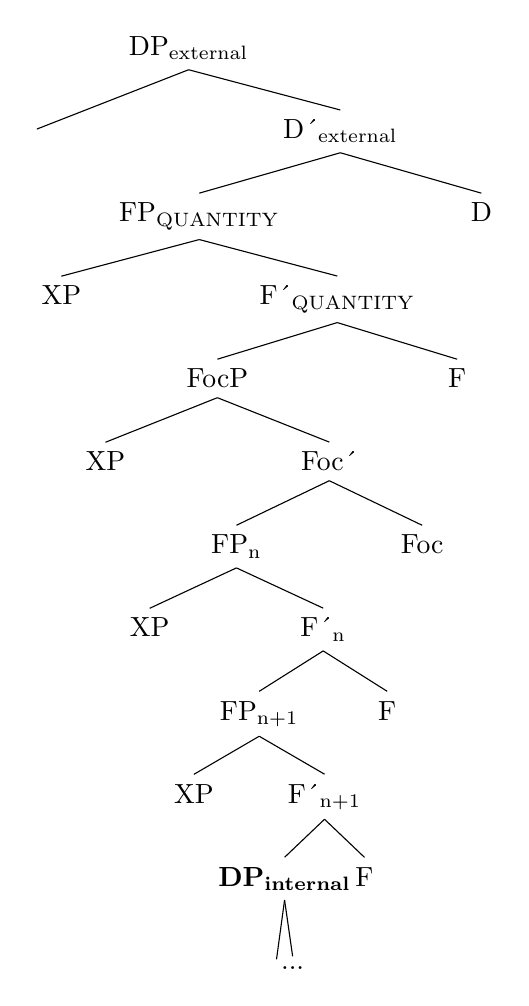
\begin{tikzpicture}[baseline=0pt, remember picture]
\tikzset{level distance=30pt, sibling distance=-5pt}
 \Tree [.DP\textsubscript{external} {} [.D´\textsubscript{external} [.FP\textsubscript{QUANTITY} XP [.F´\textsubscript{QUANTITY} [.FocP XP [.Foc´ [.FP\textsubscript{n} XP [.F´\textsubscript{n} [.FP\textsubscript{n+1} XP [.F´\textsubscript{n+1} [.\textbf{DP\textsubscript{internal}} {} ... ] F ] ] F ] ] Foc ] ] F ] ] D ]]
\end{tikzpicture}
 \end{subfigure}
 \begin{subfigure}{0.5\textwidth}
 \centering
 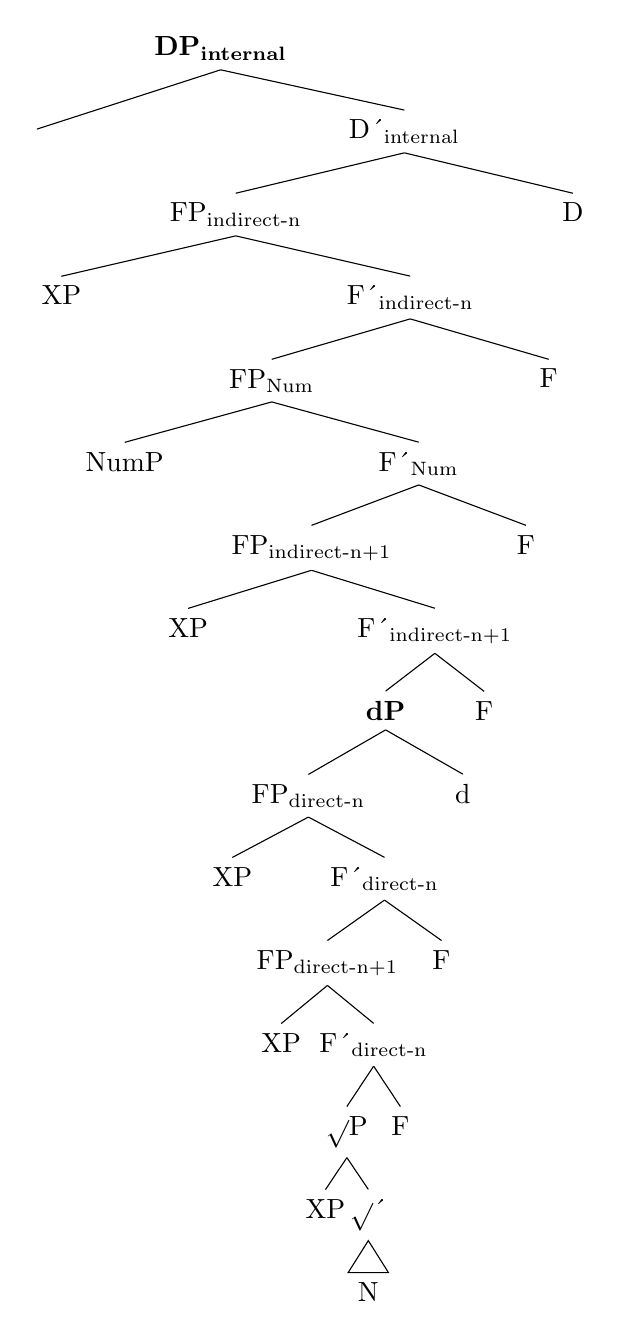
\begin{tikzpicture}[baseline=0pt, remember picture]
\tikzset{level distance=30pt, sibling distance=-5pt}
 \Tree [.\textbf{DP\textsubscript{internal}} {} [.D´\textsubscript{internal} [.FP\textsubscript{indirect-n} XP [.F´\textsubscript{indirect-n} [.FP\textsubscript{Num} NumP [.F´\textsubscript{Num} [.FP\textsubscript{indirect-n+1} XP [.F´\textsubscript{indirect-n+1} [.\textbf{dP} [.FP\textsubscript{direct-n} XP [.F´\textsubscript{direct-n} [.FP\textsubscript{direct-n+1} XP [.F´\textsubscript{direct-n} [.$\sqrt{}$P XP [.$\sqrt{}$´ \edge[roof]; {N} ] ] F ] ] F ] ] d ] F ] ] F ] ] F ] ] D ] ]
\end{tikzpicture}
 \end{subfigure}
 \caption{Structure of the Japanese DP}
 \label{fig:Structure of the Japanese DP1}
\end{figure}

%\newpage


I adopt a split-DP approach \citep{laenzlinger:2005:french, laenzlinger:2011:elements, kim:2019:syntax} and propose that the Japanese DP consists of a DP-external domain, the left periphery, and a DP-internal domain. The DP-internal domain consists furthermore of a domain for indirect (predicative) and a lower domain for direct (attributive) modification. Those two domains are separated by the indefinite head d.\footnote{The head d is the small indefinite head of a relative clause if there is one in the structure \citep{cinque:2010:adj, cinque:2020:relcl}. See chapter \ref{indefinitedpdiscussion} for discussion.} Note that the DP-external domain is represented by the left part of the tree, and the DP-internal domain is represented on the right part. The thresholds between the three domains are depicted in boldface.

This book focuses on the DP-internal domain, but a discussion on the left periphery can be found in Chapter \ref{externaldp} where I show that this area must encompass landing sites for quantificational modifiers, non-restrictive relative clauses and focused modifiers, but that essentially all types of modifiers can move there.

Modifiers, unequivocally depicted as XPs in figure \Ref{fig:Structure of the Japanese DP1}, merge in the specifier position of functional projections (FPs) within the DP. A crucial assumption that differentiates the system defended here from accounts such as \citet{cinque:2010:adj, cinque:2020:relcl} is that functional projections (with one exception) are not dedicated to specific semantic categories in the direct domain, and neither to different sizes of relative clauses in the indirect domain. In other words, these functional projections are unspecific. The labels \textit{n}, \textit{n+1}, are meant to depict that there is potentially an infinite number of functional projections inside every domain, but that there is a hierarchy, depicted by the numbers and the ``plus“ symbol.

\subsection{Unspecified functional projections predict free order}

I propose that this is the general DP spine valid in every language, but that cross-linguistic variation should be permitted concerning the nature of the functional projections present in that spine. Some languages, including English, have the relevant language-specific tools, called \textit{Units of Language} in \citet{wiltschko:2014:universal}, available to create functional projections dedicated to fine-grained semantic categories such as \textsc{shape} or \textsc{color}. In turn, this lead to the familiar ordering restrictions within the direct domain. %\is{units of language}

In turn, Japanese modifiers are licensed by functional heads in the respective domains they belong to, but this language lacks the language-specific tools to form \textit{dedicated} functional projections. Since modifiers are not merged in such dedicated, and rigidly ordered, functional projections, their merging position is not predetermined and hence they can occur in any order. As a result, even for a pair of non-predicative modifiers, which should exhibit ordering restrictions given what we know from other languages, no such ordering restrictions are observable.

This is illustrated below for the two modifiers of \textsc{nationality} \textit{Denmāku-no} `Danish’ and of \textsc{material} \textit{chīku-no} `teak’. Their two possible surface orders are simply the result of different merging positions within the DP. See Chapter \ref{discussiondirect} for discussion on ordering in the direct domain.

\newpage

\ex. \ag. Denmāku-no chīku-no isu\\
Denmark-\textsc{no} teak-\textsc{no} chair (= \ref{denmaku2})\\
\b. 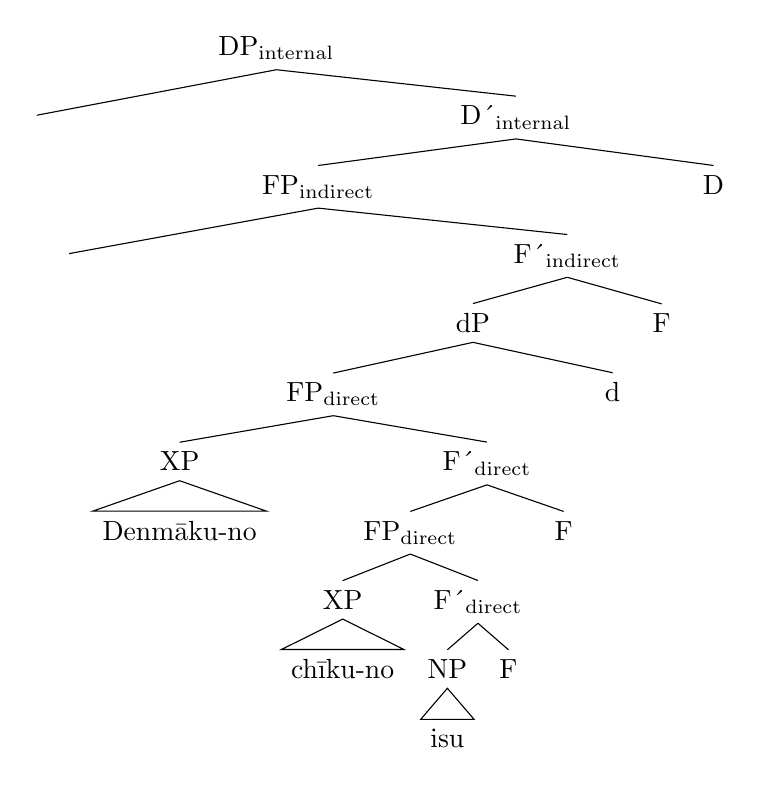
\begin{tikzpicture}[baseline=0pt, remember picture]
\tikzset{level distance=25pt, sibling distance=5pt}
\Tree [.DP\textsubscript{internal} {} [.D´\textsubscript{internal} [.FP\textsubscript{indirect} {} [.F´\textsubscript{indirect} [.dP [.FP\textsubscript{direct} [.XP \edge[roof]; Denmāku-no ] [.F´\textsubscript{direct} [.FP\textsubscript{direct} [.XP \edge[roof]; chīku-no ] [.F´\textsubscript{direct} [.NP \edge[roof]; isu ] F ] ] F ] ] d ] F ] ] D ] ]
\end{tikzpicture}

\ex. \ag. chīku-no Denmāku-no isu\\
teak-\textsc{no} Denmark-\textsc{no} chair (= \ref{denmaku3})\\
\b. 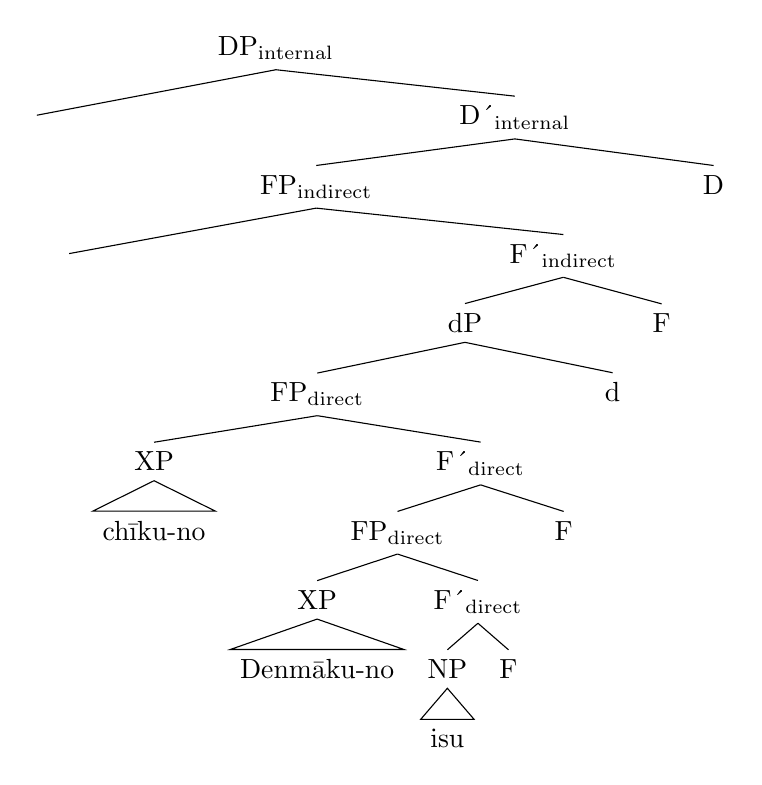
\begin{tikzpicture}[baseline=0pt, remember picture]
\tikzset{level distance=25pt, sibling distance=5pt}
\Tree [.DP\textsubscript{internal} {} [.D´\textsubscript{internal} [.FP\textsubscript{indirect} {} [.F´\textsubscript{indirect} [.dP [.FP\textsubscript{direct} [.XP \edge[roof]; chīku-no ] [.F´\textsubscript{direct} [.FP\textsubscript{direct} [.XP \edge[roof]; Denmāku-no ] [.F´\textsubscript{direct} [.NP \edge[roof]; isu ] F ] ] F ] ] d ] F ] ] D ] ]
\end{tikzpicture}

Concerning indirect modifiers, a similar situation holds. They only come in one size in Japanese, namely CP, which means Japanese only has one type of (head-external) relative clause. Again, this predicts the absence of ordering restrictions, also within the indirect domain. However, the indirect domain also encompasses a projection for numerals and in principle, indirect modifiers can occur in a position above or below the relevant projection hosting numerals. %\is{numerals}

\ex. \ag. [pātī-de at-ta [futari-no josei]]\\
party-\textsc{loc} meet-\textsc{pst} two-\textsc{no} woman\\
\bg. [futari-no [pātī-de at-ta josei]]\\
two-\textsc{no} party-\textsc{loc} meet-\textsc{pst} woman\\
`the two women who I met at a party'

Furthermore, indirect modifiers of higher complexity, for instance if they contain an overt subjects or adverbials, are more natural in a higher position.

\ex. \ag. [doresu-ga utsukushi-k-at-ta [futari-no josei]]\\
dress-\textsc{nom} beautiful-\textsc{pred-cop-pst} two-\textsc{no} woman\\
\bg. \#[futari-no [doresu-ga utsukushi-k-at-ta josei]]\\
two-\textsc{no} dress-\textsc{nom} beautiful-\textsc{pred-cop-pst} woman\\
`the two women whose dresses were beautiful'

This suggests that indirect modifiers originate low, in a position below FP\textsubscript{Num}, but can move up. This discussion will be picked up in Chapter \Ref{complexity}.

\subsection{Internal structure of modifiers}

The final hypothesis concerns the internal structure of modifiers. Following \citet{nishiyama:1999:adj}, I analyze complex elements such as \textit{katta}, given in \ref{taka-kattaoben} as combinations of two copulas and a tense marker along the following lines. This analysis will be outlined in Chapter \Ref{copulaelements}. %\is{copula}

\exg. ano taka-k-at-ta doresu\\
that expensive-\textsc{pred-cop-pst} dress\\
`that dress which was expensive' \null \hfill \textit{i}-adjective, past

On the other hand, the monomoraic elements co-occurring with Japanese non-verbal modifiers in attributive position are not manifestations of copulas and tense markers. Rather, I argue that these elements, exemplified below with \textsc{no}, are overt manifestations of a syntactic head labeled \textsc{mod} \citep{rubin:1994:mod}. This proposal is similar to the Mod-Insertion hypothesis of \citet{kitagawa:1982:prenominal}, but crucially does not assume post-syntactic insertion. Instead, \textsc{mod} has a syntactic function and licenses the preceding modifier in attributive position along the following lines illustrated with a direct modifier.

\newpage

\ex. \label{tadanogakuseitree} \ag. kono tada-no gakusei\\
this mere-\textsc{mod} student\\
`this mere student’
\b. 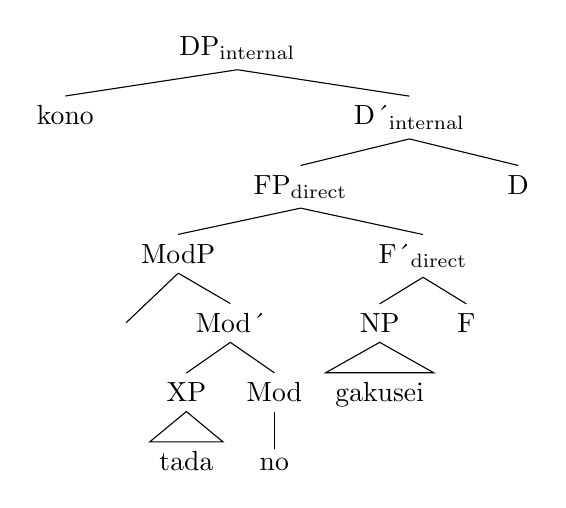
\begin{tikzpicture}[baseline=0pt, remember picture]
\tikzset{level distance=25pt, sibling distance=5pt}
 \Tree [.DP\textsubscript{internal} kono [.D´\textsubscript{internal} [.FP\textsubscript{direct} [.ModP {} [.Mod´ [.XP \edge[roof]; tada ] [.Mod no ] ] ] [.F´\textsubscript{direct} [.NP \edge[roof]; gakusei ] F ] ] D ]]
\end{tikzpicture}

I argue for a unified analysis of \textsc{no} which is not contingent on the nature of the different elements that precede it. Furthermore, also the elements following adjectives are instances of such a syntactic head, which means its spell-out form is contingent on the word class of the preceding modifier. Readers interested in this discussion are referred to Chapter \ref{internalstructure}.

\section{The Japanese nominal domain} \label{intro japanese}

In this section, I will present the characteristics of the Japanese language that are relevant for this book. I focus on the nominal domain and nominal modifiers.

\subsection{General information and word classes}

Japanese is the first language of approximately 125 million people and the official language in Japan and certain regions of Palau. It is a strictly head-final SOV language in which the verb cannot be moved from sentence-final position (\citealt{kuno:1973:structure, martin:1975:reference, iwasaki:2013:japanese} among others). Another key feature is its agglutinative character. Grammatical information is encoded via affixes, predominantly suffixes. %\is{word classes}

There is a classical divide between inflecting and uninflecting, as well as dependent and independent word classes,\footnote{Following the terminology of \citet{spencer:2020:uninflectedness}, \textit{inflecting} denotes all those word classes in a specific language whose members generally do inflect. \textit{Uninflecting} denotes word classes whose members never inflect, while \textit{uninflectable} denotes specific members of an otherwise inflecting word class that for various reasons do not inflect.} making \textit{inflection} a key characteristic for differentiating between word classes. What is meant by this term is not the familiar morphological alternation dependent on categories such as number or person, rather inflection (Japanese: \textit{katsuyō} 活用) denotes the conjugation of verbal categories in different inflectional forms. These inflectional forms. or \textit{katsuyōkei} (活用形). not only encode different functions, they are also encoded for which functional, or lexical, elements they host.\footnote{Six inflectional forms are recognized on the basis of Classical Japanese: I \textit{mizenkei} 未然形 (negative form/irrealis), II \textit{renyōkei} 連用形 (nominalization/adverbial form), III \textit{shūshikei} 終止形 (sentence-final form, also conclusive), IV \textit{rentaikei} 連体形 (attributive form), V \textit{izenkei} 已然形 (concessive form) and VI \textit{meireikei} 命令形 (imperative form). These forms and the respective terminology are still referred to with regard to Modern Japanese, but the amount and nature of these inflectional forms is subject to debate. This is because for many inflectional paradigms, the different forms have become syncretic and hard to distinguish (see \citealt{kohlich:2023:uninflecting} for an overview). Furthermore, strong phonological processes have blurred the borders of inflectional form and suffix making inflection appear almost fusional. Some clear instances of inflectional forms can be observed for verbs of the \textit{consonant inflectional paradigm}, for example \textit{nom} `to drink'. Compare the following stem vowel alternations.

\par

\ex. \ag. nom-\textbf{u}\\
drink-\textsc{prs}\\
`I/you/etc. drink' \null \hfill sentence-final
\bg. nom\textbf{i}-ta-i\\
drink-\textsc{vol}-\textsc{prs}\\
`I/you/etc. want to drink' \null \hfill nominalization
\cg. nom\textbf{e}-ba\\
drink-if\\
`if I/you/etc. drink' \null \hfill concessive

\par


Note also that I use the glosses \textsc{shk} (\textit{shūshikei}), \textsc{rtk} (\textit{rentaikei}) and \textsc{ryk} (\textit{renyōkei}) mostly with reference to Classical Japanese and only when relevant with reference to Modern Japanese.} Inflecting word classes include verbs, the two adjective classes and the functional category of so-called \textit{auxiliary verbs} (Japanese: \textit{jodōshi} 助動詞).\footnote{As will become obvious on multiple occasions, it is a matter of debate whether \textit{na}-adjectives do inflect (see \citealt{uehara:1998:syntactic, kishimoto:2016:lexical}).}

\subsection{Modifiers and modification}

The strict head-finality is also apparent in the nominal domain. Modifiers exclusively precede the noun and include numerals, verbs, nominals, two adjective groups, and demonstratives, but not articles. The two adjective groups, in Japanese called \textit{keiyōshi} 形容詞, lit. `qualifying words’, will consistently be referred to as \textit{\textit{i}-adjectives} and \textit{\textit{na}-adjectives} throughout this book reflecting their systematic morphological differences. \textit{i}-adjectives such as \textit{taka-i} `high, expensive’ end in -\textsc{i} in attributive position, but also in predicative position to mark non-past, whereas \textsc{na}-adjectives such as \textit{shikku-na} `chic’ end in -\textsc{na} in attributive position in non-past. In predicative position, they exhibit the form -\textsc{da}, and this difference essentially reflects the difference between \textit{shūshikei}, the sentence-final form, and \textit{rentaikei}, the attributive form, of Classical Japanese.\footnote{This difference has been reduced in all other inflecting word classes since around Late Middle Japanese (12–16 AD), when the attributive form started to appear in sentence-final environments. The dichotomy is still observable for inflecting word classes in the different varieties of Okinawan (Ryūkyūan), which go back to the same origin as Japanese, but in many instances have preserved features of Proto-Japanese.}

Thus \textit{na}-adjectives, in non-past, alongside nouns to be reviewed below, provide one exception to the observation that Japanese lexemes always appear in the same form in attributive and in predicative position. %\is{Japanese adjectives}

\ex. \ag. Ano doresu-wa shikku-da.\\
that dress-\textsc{top} chic-\textsc{da}\\
`That dress is chic.'
\bg. ano shikku-na doresu\\
that chic-\textsc{na} dress\\
`that chic dress' \null \hfill \textit{na}-adjective, non-past

\subsection{Adjectives, I and NA} \label{chapter 1, i and na}

The two adjective groups exhibit the typical differences observable in languages with two adjective groups \citep{dixon:2004:adj}. \textit{i}-adjectives are the older group and most lexemes belong to the native Japanese stratum, whereas \textit{na}-adjectives entered the language in Late Middle Japanese and have only received the status as an independent word class in the middle of the 20th century (\citealt{kato:2003:nihongo, lewin:2003:abriss, frellesvig:2010:history} a.o.). Most lexemes of this adjective class belong to non-native, foreign strata, mostly Sino-Japanese, but also English, but there are also some native lexemes, then often with typical endings -\textit{ka}, -\textit{raka} or -\textit{yaka} (see for instance \citealt[210–213]{uehara:1998:syntactic} for diachronic differences). This also means that \textit{na}-adjectives present an open class, accepting new loanwords, while \textit{i}-adjectives are a closed class.

As for their semantics, \textit{i}-adjectives typically express basic notions. More detailed meanings are denoted via \textit{na}-adjectives. However, both groups can in principle express all semantic categories of various well-known hierarchies (\citealt{scott:2002:stacked} among others), although some categories are biased towards one group. More basic categories such as \textsc{dimension} show a higher percentage of \textit{i}-adjectives, the more versatile category \textsc{quality} incorporates more \textit{na}-adjectives \citep{uehara:1998:syntactic}. %\is{Japanese adjectives}

There exist various analyses of the monomoraic elements \textsc{i} and \textsc{na}. Until the 2000’s, \textsc{i} was analyzed either as an inflecting tense morpheme \citep{teramura:1982:nihongo, murasugi:1991:noun, urushibara:1993:syntactic, uehara:1998:syntactic}, or (part of) a copula \citep{kubo:1992:japanese}. \textsc{na} on the other hand was perceived less controversially and predominantly analyzed as the copula, alongside its predicative equivalent \textsc{da}, which generally received unequivocal copula-status (for example \citealt{urushibara:1993:syntactic, nishiyama:1999:adj}). One reason for this is that not only \textsc{da}, but also the attributive \textsc{na}, can be paraphrased by the complex element \textsc{dearu}, which has been identified as the canonical form of the copula and is historically related to \textsc{da} (see for example \citealt{urushibara:1993:syntactic, nishiyama:1999:adj, nakahara:2002:japanese}; see \citealt{miyama:2011:da} for historical evidence). This is shown below.\footnote{The two elements do not display a significant difference in meaning, but \textsc{dearu} is mostly observed in written register and rarely in spoken language. It is also degraded in attributive position, although not impossible. I will gloss both elements simply as \textsc{cop} for now. For the relevant analysis see Chapter \ref{copulaelements}.}

\ex. \ag. Ano doresu-wa shikku-dearu.\\
that dress-\textsc{top} chic-\textsc{cop}\\
`That dress is chic.'
\bg. ano shikku-dearu doresu\\
that chic-\textsc{cop} dress\\
`that dress which/that is chic' \\ \null \hfill \textit{na}-adjective, non-past with copula \textsc{dearu}

Furthermore, both adjective groups can express past, and when they do, they exhibit the same complex morphological forms in attributive as in predicative position, meaning the formerly observed difference in the case of \textit{na}-adjectives vanishes. \textit{na}-adjectives co-occur with the complex element \textsc{deatta}, which corresponds to \textsc{dearu} in non-past, or the shorter form \textsc{datta}, where the syllable /e/ has been reduced and which corresponds to \textsc{da}.\footnote{Same as \textsc{dearu} and \textsc{da}, these two forms display a difference in register, but are otherwise interchangeable.}

\textit{i}-adjectives on the other hand seem to truly inflect for past. The complex element \textsc{katta} occurs instead of \textsc{i}, again in both attributive and predicative position. At first glance, these two elements seem to not bear any resemblance to one another. %\is{copula}

\ex. \ag. Ano doresu-wa shikku-d(e)atta.\\
that dress-\textsc{top} chic-\textsc{cop.pst}\\
`That dress was chic.'
\bg. ano shikku-d(e)atta doresu\\
that chic-\textsc{cop.pst} dress\\
`that dress which was chic' \null \hfill \textit{na}-adjective, past

\ex. \label{taka-katta} \ag. Ano doresu-wa taka-katta.\\
that dress-\textsc{top} expensive-\textsc{pst},\\
`That dress was expensive.'
\bg. ano taka-katta doresu\\
that expensive-\textsc{pst}, dress\\
`that dress which was expensive' \null \hfill \textit{i}-adjective, past

A landmark analysis to be adopted in this study comes from \citet{nishiyama:1999:adj}, who aimed at a unifying analysis of \textsc{i} and \textsc{na} as combinations of two copulas and a tense marker. This analysis, although its adoption at face value brings about some problems, is important in the sense that it offers a parallel analysis of the two elements. In earlier studies, often, but not always \citep{backhouse:1984:have}, the dichotomy between \textit{inflecting tense marker} (\textsc{i}) vs. \textit{copula} (\textsc{na}) reflected the word class status of relevant lexemes, \textit{i}-adjectives were analyzed as (verbal) inflecting predicates, and \textit{na}-adjectives as non-inflecting nouns (see most of all \citealt{uehara:1998:syntactic}).

What should be pointed out, however, is that the modifiers that co-occur with \textsc{i} and \textsc{na} are adjectives.\footnote{The fact that \textit{i}-adjectives seem rather ``verby’’ and \textit{na}-adjectives rather ``nouny’’ has prompted several researchers to subsume them under the headlines of \textit{Verbals} and \textit{Nominals} \citep{uehara:1998:syntactic}, sometimes denying the adjective category in Japanese in general \citep{wetzer:1996:typology}. In fact, the analysis of \citet{nishiyama:1999:adj} and its subsequent incorporation in the study of \citet{baker:2003:cat} were important steps towards the assumption of two adjective groups in Japanese.} First, note that, abstracting away from semantic reasons, such lexemes are typically gradable as exemplified for a \textit{na}-adjective below. Gradability is a typical feature of the adjectival category \citep{baker:2003:cat, dixon:2010:grammatical} and in Japanese expressed via comparative-formation with the particle \textit{yori(-mo)} `than' and the optional adverb \textit{motto} `more' \ref{machi-yori}, degree adverbs \ref{totemonigiyaka}, or superlative-formation via the adverb \textit{ichi-ban} `most' (Lit. `one-number') \ref{machi-ichiban}, see \citet{bhatt:2011:reduced}.

%\newpage

\ex. \ag. Kono machi-wa ano machi-yori (motto) nigiyaka-da\\
this city-\textsc{top} that city-than (more) lively-\textsc{cop}\\
`This city is more lively than that city.’ \label{machi-yori}
\bg. totemo nigiyaka-na machi\\
very lively-\textsc{na} city\\
`very lively city' \label{totemonigiyaka}
\cg. ichi-ban nigiyaka-na machi\\
number-one lively-\textsc{na} city\\
`the most lively city' \label{machi-ichiban}

Another, more language-specific, feature, of adjectivehood is nominalization with the suffix -\textsc{sa} `-ness’, which only nominalizes adjectives, but never nouns, since they are already nominal. As shown below, \textit{i}-adjectives (\textit{samu-i} `cold’) and \textit{na}-adjectives (\textit{shizuka-na} `quiet’) can be nominalized, but nouns (\textit{sensei} `teacher’) or verbs (\textit{tabe} `eat’) cannot.\footnote{See \citet{teramura:1982:nihongo, wenck:1974:systematische, urushibara:1993:syntactic, rickmeyer:1995:japanische, kato:2003:nihongo, muraki:2012:nihongo} for a similar application of this characteristic. Other, more specific suffixes which only attach to adjectives are -\textit{garu}, which derives verbs from adjectives that express (often negative) physiological or psychological states \citep{urushibara:1993:syntactic}, and the verbal suffix -\textit{sugiru} `to exceed; too’.}

%\newpage

\ex. \ag. samu-sa\\
cold-ness\\
\bg. shizuka-sa\\
quiet-ness\\
\cg. *sensei-sa\\
teacher-ness\\
\dg. *taberu-sa\\
eat-ness\\

Another characteristic differentiating adjectives from nouns is the inability to appear with particles, especially -\textsc{ga} for nominative and -\textsc{wo} for accusative case \citep{suzuki:1972:nihon, martin:1975:reference, teramura:1982:nihongo, nakayama:2004:tokubetsu, muraki:2012:nihongo}, in other words the lack of \textit{referential use} \citep{oshima:2019:gradability}, as shown below.

\ex. \ag. *Samu-(i-)ga ku-ru.\\
cold-\textsc{nom} come-\textsc{prs}\\
(`(The/An) cold comes’.)
\bg. *Samu-(i-)wo mi-ru.\\
unknown-\textsc{acc} see-\textsc{prs}\\
(`to see (the/a) cold’) \null \hfill \textit{i}-adjective

%\newpage

\ex. \ag. *Shizuka-ga ku-ru.\\
quiet-\textsc{nom} come-\textsc{prs}\\
(`(The/An) quiet comes.’)
\bg. *Shizuka-wo mi-ru.\\
quiet-\textsc{acc} see-\textsc{prs}\\
(`to see (the/a) quiet’) \null \hfill \textit{na}-adjective

\subsection{\textit{no}-Modifiers and \textsc{NO}}

The discussion above was meant to show that \textsc{i} and \textsc{na} co-occur only with adjectives. This subsection discusses the monomoraic element \textsc{no}, whose distribution is not restricted to a specific word class.

\subsubsection{Nouns}

In most grammars of Japanese, \textsc{no} is strongly, often exclusively, connected to the co-occurrence with nouns. In fact, nouns share their entire inflectional paradigms with \textit{na}-adjectives, except for this element which they co-occur with in attributive position, contrary to the element \textsc{na} that co-occurs with \textit{na}-adjectives. The prototypical relationship between two nouns connected via \textsc{no} is arguably possession, which explains why this element is predominantly glossed as \textsc{gen}.\footnote{For discussion and different opinions see \citet{murasugi:1991:noun, uehara:1998:syntactic, backhouse:2004:inflected}. I will gloss it as \textsc{no} until I present the proper analysis as a syntactic head in Chapter \ref{internalstructure}.} %\is{\textit{no}-modifiers}

\ex. \label{senseino} \ag. sensei-no hon\\
teacher-\textsc{no} book\\
`book of the teacher'
\bg. Tarō-no jitensha\\
Taro-\textsc{no} bicycle\\
`Taro’s bicycle’ \null \hfill noun, possessive

The lexemes combined via \textsc{no} in \ref{senseino} are clearly nouns. Syntactically, they can appear with case particles as visible in \ref{noun reference}, from a semantic and pragmatic point of view, they establish a \textit{reference} to some entity, most obvious with the proper name \textit{Tarō}, alongside common ground between speaker and hearer.

\exg. sensei / Tarō / jitensha / hon-wo mi-ta\\
teacher / Taro / bicycle / book-\textsc{acc} see-\textsc{pst}\\
`saw the teacher / Tarō / the/a bicycle / the/a book’ \label{noun reference}

Several other relationships can be invoked when two nouns are connected via \textsc{no}, prominently argument roles \citep{murasugi:1991:noun}. The following example is ambiguous between a subject and an object reading.

\exg. Itaria-no hakai\\
Italy-\textsc{no} destruction\\
1. `Italian destruction' \null \hfill (= destruction by Italy, \textit{subject})\\
2. `Italian destruction' \null \hfill (= destruction of Italy, \textit{object})

A subject and an object can even appear side by side within the same DP, both times followed by \textsc{no}. Usually (abstracting away from meaning), the reading where the first noun is interpreted as the subject is more accessible, but permutation is naturally possible.\footnote{Examples of multiple occurrences of \textsc{no} also show that it is recursive in the sense that in theory an infinite number of elements can be connected via \textsc{no} in the same DP. This is similar to English \textit{of} or genitive -\textit{s}, with the difference that two or more argument genitives are not allowed in one DP as also visible in the translations of the relevant example \citep[86]{murasugi:1991:noun}.}

\exg. yabanjin-no toshi-no hakai\\
barbarian-\textsc{no} city-\textsc{no} destruction\\
`the destruction of the city by the barbarians’ \hfill \citep[7]{murasugi:1991:noun}

These DPs can be paraphrased as sentences where the modifying nouns bear nominative and accusative case particles and the modified noun forms a predicate with the light verb \textit{su}, also showing that \textit{no} is mutually exclusive with case particles.

\exg. Yabanjin-ga toshi-wo hakai-shi-ta.\\
barbarian-\textsc{nom} city-\textsc{acc} destruction-do-\textsc{pst}\\
`The barbarians destroyed the city.’

Furthermore, \textsc{no} can license the attributive modification of nouns that bear other diverse argument roles. In this case, those nouns typically appear with postpositions in order to make the role they bear clearer. These postpositions include \textsc{de} (instrumental, locative), \textsc{ni} (dative, locative, allative, illative) and \textsc{kara} (ablative) \citep{murasugi:1991:noun,saito:2008:N}.\footnote{When the context is sufficiently clear, the postpositions preceding \textsc{no} can also be omitted.} Also, note that these examples give a first indication that not everything that co-occurs with \textsc{no} is a noun.\footnote{In fact, this is one argument for the often drawn distinction between case particles and postpositions. Case particles do not co-occur with \textsc{no}. Note furthermore that PPs can also co-occur with case particles, which modifiers belonging to the adjective groups can never do \citep{murasugi:1991:noun, urushibara:1993:syntactic}.}

%\newpage

 \ex. \label{no with case} \ag. ishi-de-no kōgeki\\
stone-\textsc{ins-no} attack\\
`an attack with stones' \null \hfill instrumental \citep[248]{saito:2008:N}
\bg. Tōkyō-de-no kaigi\\
Tokyo-\textsc{loc-no} meeting\\
`the meeting in Tokyo \null \hfill locative
\cg. Tōkyō-kara-no densha\\
Tokyo-\textsc{abl-no} train\\
`the train from Tokyo' \null \hfill ablative \citep[50]{murasugi:1991:noun}

Note that \textsc{no} always follows the respective postposition and must be closest to the noun, highlighting its connecting function.

\exg. *ishi-no-de kōgeki\\
stone-\textsc{no-ins} attack\\

Nouns performing modification duties do not necessarily have to bear an argument status. Sometimes they are adjuncts \ref{adjunct no}. This also includes cases of possessor-possessee relationship where the possessor appears as the second noun \ref{alienable}.

 \ex. \label{adjunct no} \ag. ame-no hi\\
rain-\textsc{no} day\\
`rainy day' \null \hfill \citep[251]{saito:2008:N}
\cg. otoko-no ko\\
man-\textsc{no} child\\
`male child (=boy)'
\cg. kuruma-no zasshi\\
car-\textsc{no} magazine\\
`magazine about cars' \null \hfill adjuncts

\ex. \label{alienable} \ag. megane-no gakusei\\
glasses-\textsc{no} student\\
`the student with glasses'
\bg. shiraga-no gakusei\\
white.hair-\textsc{no} student\\
`the student with white hair' \\ \null \hfill \citep[96]{kato:2003:nihongo}

\subsubsection{Adjectival Modification}

Although most Japanese grammars (\citealt{iwasaki:2013:japanese, tsujimura:2014:intro, hasegawa:2015:japanese} etc.), including the so-called \textit{school grammar} (\citealt{hashimoto:1948:kokugogaku})), treat lexemes preceding \textsc{no} as nouns, \textsc{no} is not restricted to the lexical class of nominals, but is also involved in (qualitative) adjectival modification \citep{muraki:2012:nihongo, oshima:2019:gradability}. A good example is offered with the lexeme \textit{mumei-no} `unknown’, which appears (almost) exclusively with \textsc{no}, but exhibits clear characteristics of adjectivehood. These include gradability, at least with adverbs such as \textit{kanzenni} `completely’ \ref{kanzennimumei} and inside comparative clauses \ref{yorimumei}, the possibility to be nominalized via the suffix -\textsc{sa} `-ness’ \ref{mumeisa}, and the impossibility to appear with nominative and accusative case particles, \ref{mumei-ga} and \ref{mumei-wo}. For these reasons, such lexemes are sometimes referred to as \textit{no-adjectives} \citep{mio:1942:hanashi, mio:1958:hanashi, muraki:2012:nihongo}, making them a third morphological subgroup of the adjectival category in Japanese (for different analyses of \textit{mumei-no} see \citealt{teramura:1982:nihongo, kato:2003:nihongo, morita:2013:morph}, for an overview see \citealt{kohlich:2023:suppl}). %\is{Japanese adjectives}

\ex. \ag. mumei-no haiyū\\
unknown-\textsc{no} actor\\
`unknown actor'
\bg. kanzenni mumei-no haiyū\\
completely unknown-\textsc{no} actor\\
`completely unknown actor' \label{kanzennimumei}
\cg. Tanaka-san-yori (motto) mumei-no haiyū-to at-ta.\\
Tanaka-Mr.-than more unknown-\textsc{no} actor-\textsc{com} meet-\textsc{pst}\\
`I met with a more unknown actor than Mr. Tanaka.’ \label{yorimumei}
\dg. mumei-sa\\
unknown-ness\\
`unknownness; anonymity’ \label{mumeisa}
\eg. *Mumei-ga ku-ru.\\
unknown-\textsc{nom} come-\textsc{prs}\\
(`(The/An) Unknown comes.’) \label{mumei-ga}
\fg. *Mumei-wo mi-ru.\\
unknown-\textsc{acc} see-\textsc{prs}\\
(`I see (the/an) unknown.’) \null \hfill \textit{no}-adjective \label{mumei-wo}

Importantly, lexical modifiers co-occurring with \textsc{no} are not only clear nouns or clear adjectives, but include many in-between cases. Some modifiers can occur with \textsc{na} in addition to \textsc{no}, some can occur with both and exhibit nominal use, there are also some with only occur with \textsc{na}, but are simultaneously nominals.\footnote{For more on this see Chapter \ref{corpusanalysis} below and \citet{kohlich:2023:suppl}.} I will refer to all modifiers that appear with \textsc{no} as \textit{\textit{no}-modifiers} adopting a uniform non-committal label for relevant elements.

Such lexical \textit{no}-modifiers truly share the rest of their inflectional paradigm with \textit{na}-adjectives, meaning they also appear predicatively with the copula \textsc{da}. \textsc{no} as well as \textsc{no} can be paraphrased by the canonical copula \textsc{dearu}.

\ex. \ag. Ano haiyū-wa mumei-da.\\
that actor-\textsc{top} unknown-\textsc{cop}\\
`That actor is unknown.’
\bg. Ano haiyū-wa mumei-dearu.\\
that actor-\textsc{top} unknown-\textsc{cop}\\
`That actor is unknown.’
\cg. ano mumei-dearu haiyū\\
that unknown-\textsc{cop} actor\\
`that unknown actor’

%\newpage

\subsubsection{Functional Elements} \label{grammatical no}

Besides lexical elements, all functional elements which serve as nominal modifiers, are connected to the head noun via \textsc{no}. This holds for most quantifiers, perhaps an in-between case between lexical and functional modifiers.\footnote{Eventually, I will treat quantifiers as lexical elements. See Chapter \ref{quantificational modifiers}.}

\exg. takusan-no / subete-no gakusei\\
a.lot-\textsc{no} / all-\textsc{no} student\\
`many / all students' \hfill \null quantifiers

Clear functional elements that can appear as attributive modifiers in Japanese are wh-elements \ref{wh no} (see for instance \citealt{watanabe:2001:wh}) and classifiers, which follow numerals \ref{classifier no} (\citealt{saito:2008:N}).

\exg. Doko-no ATM-de shukkin deki-mas-u ka.\\
where-\textsc{no} ATM-\textsc{loc} withdraw can-\textsc{aux.pol-prs} \textsc{q}\\
`At which ATMs can you withdraw?’ (Lit. `At ATMs where...’) \label{wh no} \footnote{\url{https://help.jibunbank.co.jp/faq_detail.html?id=182, 2023/02/05}.} \\ \null \hfill wh-elements

 \ex. \label{classifier no} \ag. san-bon-no bīru\\
three-\textsc{cl-no} beer\\
`three bottles of beer’ \label{sanbon}
\bg. go-nin-no gakusei\\
five-\textsc{cl-no} student\\
`five students’ \null \hfill numeral classifiers

\textsc{no} is also the final mora of demonstratives of the type \textit{kono} `this’, but here has a bound character in Modern Japanese.

\exg. kono / sono / ano / dono hon\\
this.\textsc{hearer-proximate} / that.\textsc{speaker-proximate} / that.\textsc{distal} / which book\\
`this / that / that (over there) / which book'

\subsubsection{Analysis of NO}

Compared to \textsc{i} and \textsc{na}, the status of \textsc{no} is more versatile and harder to pinpoint. The question is whether every instance of \textsc{no} can be reduced to a single function, at least DP-internally, or whether different instances of \textsc{no} should be postulated. Possible analyses of \textsc{no} are outlined in detail in Chapter \ref{comparisonpreviousno}, but this book attempts at a unified analysis of \textsc{no}, namely as a syntactic head that licenses modification. The analysis depicted in \ref{tadanogakuseitree} can therefore be applied to all examples mentioned in this section.\footnote{One exception are the demonstratives of the type \textit{kono} `this’ which will be treated as specifiers of D-heads reflecting standard assumptions in syntactic research on Japanese.} For instance a numeral (containing a classifier) would be integrated as follows. %\is{Mod}

\ex. \ag. san-bon-no bīru\\
three-\textsc{cl-mod} beer\\
`three bottles of beer’ \null \hfill (= \ref{sanbon})
\b. 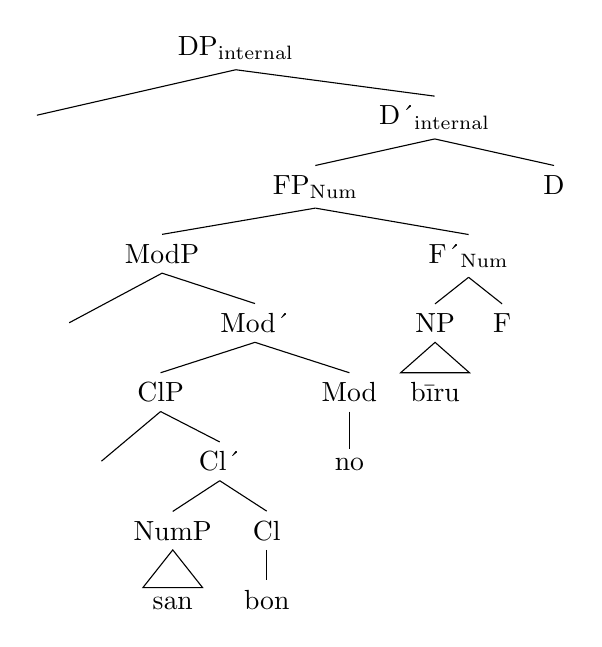
\begin{tikzpicture}[baseline=0pt, remember picture]
\tikzset{level distance=25pt, sibling distance=5pt}
 \Tree [.DP\textsubscript{internal} {} [.D´\textsubscript{internal} [.FP\textsubscript{Num} [.ModP {} [.Mod´ [.ClP {} [.Cl´ [.NumP \edge[roof]; {san} ] [.Cl bon ] ] ] [.Mod no ] ] ] [.F´\textsubscript{Num} [.NP \edge[roof]; bīru ] F ] ] D ]]
\end{tikzpicture}

\subsubsection{Where \textsc{NO} is not used} \label{no no}

It seems that \textsc{no} appears in all instances of (non-adjectival) modification, which is why it is often treated similar to Mandarin \textsc{de} (see \citealt{saito:2008:N}). However, it is illicit after verbal relative clauses including a finite (past or non-past) verb (see for instance \citealt{murasugi:1991:noun, saito:2008:N}).

\ex. \ag. kare-ga kat-ta (*no) hon\\
he-\textsc{nom} buy-\textsc{pst} \textsc{no} book\\
`the book that he bought’
\bg. hon-wo yon-de-i-ru (*no) gakusei\\
book-\textsc{acc} read-\textsc{ger}-be-\textsc{prs} \textsc{no} student\\
`the student who is reading a book’

Similarly, \textsc{no} never appears after complex morphological past forms, which also contain a tensed form.

\exg. ano shizuka-datta (*no) yoru\\
that quiet-\textsc{cop.pst} \textsc{no} night\\
`that night which was quiet’

Furthermore, it is never the case that any of the elements \textsc{no}, \textsc{na} and \textsc{i} co-occur.

\exg. aka-i (*no) hana\\
red-\textsc{i} \textsc{no} flower\\
`red flower'

\exg. kanzen-na (*no) baka\\
complete-\textsc{na} \textsc{no} idiot\\
`complete idiot'

Finally, \textsc{no} is never possible in predicative position.\footnote{The form \textit{no-da} exists, however in this case \textit{no} is an emphatic element whose usage domain is pragmatically restricted.}

\exg. Ano haiyū-wa mumei (*no) da.\\
that actor-\textsc{top} unknown \textsc{no} \textsc{cop}\\
`That actor is unknown.’

%\newpage

\section{Data Collection} \label{corpusanalysis}

The theoretical insights of this book are mainly based on an empirical analysis in the Balanced Corpus of Contemporary Written Japanese (BCCWJ).\footnote{\url{https://chunagon.ninjal.ac.jp/auth/login} \citep{maekawa:2014:bccwj}.} All relevant materials are saved at the following repository: \url{https://osf.io/u9txp/}. I have analyzed approximately 2300 lexemes which were predominantly collected from the scientific literature, in total from a body of 23 different studies. The categories according to which I incorporated these lexemes were either \textit{(alleged) inability to be used predicatively} or \textit{use with -no, but no clear nominal status}. This list of lexemes will be referred to as the \textit{data set}. The repository contains two files with different annotations of this data set. Data set 1 contains a list of all relevant lexemes annotated based on the judgment of each respective author for cross-referencing purposes. Data set 2 displays the frequency of each relevant variable tested for all lexemes in the corpus.\footnote{Compilation of these lexemes finished at the beginning of 2022. Subsequent analysis began in March 2022 and was finished in August 2023. Readers are referred to a research report published by the Tokyo Gakugei University at the beginning of 2022 \citep{abe:2022:no} in which all lexemes given in \citet{muraki:2012:nihongo} are analyzed for the variables \textit{attributive use, predicative use, adverbial use} and \textit{referentiality}. This is therefore a major contribution to the field and many aspects are shared between this research report and my own study although sometimes numbers diverge slightly. See the data paper for relevant details.} %\is{corpus; data collection}

The repository also contains a data paper, which in detail outlines the design and structure of the corpus and its analysis tools and depicts all necessary steps and search queries that were performed \citep{kohlich:2023:suppl}. It also gives a more detailed overview of the results of the analysis that can be granted here. Readers are welcome to replicate this study, verify the results, implement refinements and provide feedback.

My goal was to establish an overview of how big the inventory of direct, that is non-predicative, modifiers in Japanese can actually be. In this respect, one must be aware that the existing literature on this matter can only be a reference point. Approximately 75\% of the lexemes in the data set are taken from the paper collection published as a monograph by MURAKI Shinjirō \citep{muraki:2012:nihongo}. Muraki presents long (yet non-exhaustive) lists of different kinds of \textit{no}-modifiers drawn from various Japanese dictionaries, among those an important list of non-predicative lexemes \citep[96–98]{muraki:2012:nihongo}, and analyzes them according to his own introspective judgment.\footnote{The validity of introspective judgments, even with regard to seemingly well-known examples and languages, has been put into question in recent years \citep{gibson:2010:weak}, and this also applies to Japanese.} The present corpus analysis had the goal of verifying such judgments.

I therefore tested for the variable \textit{predicative use with copula} for all modifiers in the data set. A modifier was classified as direct (group 5) if it was either completely lacking predicative use, or if it yielded no more than 5 predicative occurrences vs. at least 20 attributive ones, or alternatively a ratio of 5$>$1 towards attributive use.\footnote{As a rule of thumb, only lexemes with at least 5 occurrences are reported in the data set, and only lexemes with at least 25 occurrences were categorized into one of the different groups. I am aware of the fact that fewer predicative occurrences do not automatically mean that a modifier is non-predicative, in other words direct-only. Nevertheless, a skew towards attributive use signals that this is the prototypical usage domain of a given modifier, which is why I classified relevant lexemes into this group even though they might be possible in predicative position.} The relevant numbers are given below.

\ex. \a. Direct modifiers in total: 511
\b. Out of which direct modifiers with 0 hits in predicative position: 110
\c. Out of which direct modifiers with no more than 5 hits in predicative position: 190
\d. Prototypical direct modifiers with a ratio of 5$>$1 towards attributive use: 211

Besides the goal of determining which lexemes are candidates for direct modifiers, another important goal was to point out the heterogeneous word class status of \textit{no}-modifiers. For this the following variables were investigated for each lexeme. Consult Appendix B for more information and numbers on all relevant groups.

\ex. \a. occurrences in attributive use
\b. element in attributive position: \textsc{na} or \textsc{no}
\c. referential use with case particles for subject and object
\d. nominalization

One might object that corpus data do not tell the whole story for a given phenomenon and indeed, corpora depict a representative sample of real-life language and only show what is \textit{attested}, not what is \textit{possible} or \textit{impossible}. When basing our analyses on corpus queries alone we must keep in mind that certain occurrences might be missed or even overlooked. Nevertheless, a corpus is a powerful tool to give us an overview of a language and its patterns, which in turn allows us to draw important generalizations -- if we know how to look for them. As noted in \citet[7]{desagulier:2017:corpus}, ``even if no corpus can provide access to the true, unknown law of a language, a corpus can be considered a sample drawn from this law.’’

In order to further balance out these aspects, I have also performed qualitative interviews with native speakers on several occasions and had discussions with many consultants. The discussion on direct modifiers in Chapter \ref{direct japanese} is based on a qualitative study with five native speakers to inquire their judgments on grammaticality and acceptability. The study on the position of relative clauses in Chapter \ref{indirect japanese} is also based on interviews with, three different, native speakers. All these measures were undertaken to ensure the empirical adequacy of the data and the correct theoretical implications to be drawn from them.

\chapter{Theoretical Background: Cartography} \label{theoretical background}

This chapter gives a general introduction to the theoretical background and serves as a reference to what my assumptions are based on and which amendments need to be made in Chapter \Ref{theoreticalassumptions}. The framework this book is written in is \textit{Cartography}, although it might be better to speak of a \textit{research field} or a ``\textit{research topic}'' \citep[65]{cinriz:2010:carto}. Most assumptions of this book come from works by Guglielmo Cinque \citep{cinque:1993:evidence, cinque:2010:adj, cinque:2017:micro, cinque:2020:relcl, cinque:2021:carto, cinque:2023:linearization}, but I also incorporate ideas from \citet{laenzlinger:2005:french, laenzlinger:2011:elements, laenzlinger:2015:the, svenonius:2008:position} and \citet{kim:2019:syntax}. I start by outlining the core ideas of cartography, before tending to direct and indirect modification as given by \citet{cinque:2010:adj}. I then discuss the additional approaches and close with an overview over previous studies of Japanese in the cartographic program.

\section{Basic ideas and concepts} \label{sectioncarto}

What \textit{Cartography} offers is an elaborately articulated structure, a \textit{map} staying true to its name, of the noun phrase and the clause valid in every language. This research program is an offspring of X'-modeling and its adaptation to functional heads \citep{chomsky:1986:barriers} and developed parallel to Minimalism. Following Pollock’s fine-grained universal structure of the TP area (published in \citealt{pollock:1989:verb}), the clausal spine was constantly refined, most noteworthy through Rizzi’s split-CP-hypothesis \citep{rizzi:1997:the} and the highly articulated hierarchy of adverbials across different levels of the clause in \citet{cinque:1999:adverbs}. Following the doctoral thesis of Steven \citet{abney:1987:the}, the noun phrase was in the late 90’s and early 2000’s extended with several projections as well, including projections for demonstratives \citep{bruge:2002:positions}, numerals \citep{ritter:1991:two, ritter:1993:where} as well as left-peripheral focus and topic projections \citep{dimitrova:1998:fragments, ihsane:2001:specific, aboh:2004:topic, aboh:2006:when} and of course projections for (adjectival) modifiers, the focal point of this book.\footnote{See \citet{alex:2007:nounphrase} for a large overview on the noun phrase, evidence for these projections and a historical overview of the literature.} One goal of this endeavor, and cartography in general, is to argue for a parallel structure of the clause and the noun phrase.\footnote{See \citet{cinque:1993:evidence, cinque:1999:adverbs, cinque:2010:adj, cinque:2020:relcl, rizzi:1997:the, rizzi:2004:the, cinriz:2010:carto} and for a list of publications until 2015 \citet[144–151]{cinriz:2016:functional}. As also becomes obvious there, the clause has been the locus of much more attention, and far fewer controversy.}

The essential idea of Cartography is that the extended projection of every lexical head, N and V, contains several functional heads (F) where features are encoded and which give merging and landing sites in their specifier position for lexical and functional elements. Crucially, every functional projection is specified for which element(s) it hosts. Furthermore, these functional heads are ordered, are mapped, in a hierarchy that is based on structural selection and this hierarchy, this map, is universal, thus uniform in every language. This hypothesis also entails that every functional category attested in a given language is present in the structural make-up of all languages. As of now, we have no way of knowing how many functional projections there actually are in the clause and the noun phrase \citep[154–157]{cinriz:2016:functional}.

Languages thus essentially show parametric differences only in the lexicon, not in the syntax. They differ in how (and if) they realize each functional head and its specifier in the surface structure, as well as the type of movement they admit, if any. Essentially, this has the consequence that the structure offered by cartography, although rigid at first glance and in a way the ``strongest position linguists can take" \citep[9]{bortolotto:2016:RA}, is constantly the subject of development and refinement, with every new language and micro-parameter investigated, as well as every new approach and perspective taken. This makes this research field not only highly relevant and powerful, but also extremely versatile and fluctuating.\footnote{See \citet{cinque:1993:evidence, cinque:1999:adverbs, cinque:2010:adj, cinque:2020:relcl, rizzi:1997:the, rizzi:2004:the, shlonsky:2004:form, poletto:2000:the, scott:2002:stacked, laenzlinger:2011:elements} and many more. For an overview see \citet{cinriz:2010:carto, cinriz:2016:functional}.}

\subsection{Ordering}

The rigid order of functional projections (correctly) predicts the existence of ordering restrictions of the type we saw in English in the introduction. A well-established ordering hierarchy of adjectives attested in several unrelated languages \citep{sussex:1974:the, dixon:1982:where, hetzron:1978:on} and partially attributed to cognitive factors \citep{sproat:1987:pre, sproat:1991:the} reads as follows, where the symbol `$\succ$’ means `\textit{precedes in linear order}’. %\is{adjective ordering restrictions}

\ex. \textsc{quality} $\succ$ \textsc{size} $\succ$ \textsc{shape} $\succ$ \textsc{color} $\succ$ \textsc{provenance} $\succ$ N \\ \null \hfill \citep{sproat:1991:the}

It was a central achievement of the cartographic research field (most notably \citealt{cinque:1993:evidence, scott:2002:stacked, laenzlinger:2005:french, panayidou:2013:in} and \citealt{cinque:2010:adj}) to attribute these ordering principles to structural selection, getting rid of adjunction, which cannot explain ordering preferences.

In other words, each of these semantic categories corresponds to a functional head and adjectives are merged as specifiers of the head that matches their semantic value. An adjective denoting \textsc{size} would merge in FP\textsc{size} and so on.

The hierarchical order of these heads can be represented as functional selection in a bracketing format \ref{bracketing} or as in \ref{hierarchy no bracketing} where the symbol `$>$' means `\textit{is structurally/hierarchically higher}’.\footnote{When an element A is hierarchically higher than an element B, it precedes it in structural, but not necessarily in linear order since movement operations might yet take place. The symbol `$\succ$’ means `precedes in linear order’. The same technique is applied in \citet{panayidou:2013:in}.}

\ex. [\textsc{quality} [\textsc{size} [\textsc{shape} [\textsc{color} [\textsc{provenance} [N ]]]]]] \label{bracketing}

\ex. \textsc{quality} $>$ \textsc{size} $>$ \textsc{shape} $>$ \textsc{color} $>$ \textsc{provenance} $>$ N \label{hierarchy no bracketing}

This functional hierarchy is expected to be cross-linguistically valid and was verified among others for Romance, Greek, Romanian, Welsh, Mandarin (see for example \citealt{scott:2002:stacked}, the appendix of \citealt{cinque:2010:adj} and many examples in \citealt{alex:2007:nounphrase}).

\subsection{Left-right asymmetries} \label{left-right}

A fundamental contribution of Cartography, first systematized in \citet{cinque:2005:deriving, cinque:2009:fundamental} and extended in \citet{cinque:2023:linearization, cinque:2025:superiority}, was to shed light on so-called \textit{Left-right asymmetries}. It has been a central cross-linguistic observation (see for example \citealt{rijkhoff:2002:noun}), and Greenberg's Universal 20 \citep{greenberg:1963:some}, that there is a restriction on possible orders of modifiers around a lexical head when they are all on the same side of the head: When they appear on the left side of the lexical head, they are ordered in only one specific way, but when they follow the lexical head, two orders are possible: Either the identical order maintaining linear precedence, or the mirror-image, in which the order has been reversed compared to the pre-head order. This observation was verified for the order of adjectives \citep{cinque:2009:fundamental, shlonsky:2004:form}, but for many other domains as well, including the order of adverbs as well as circumstantial and directional/locative prepositions around the verb \citep[167–168]{cinque:2009:fundamental}. %\is{left-right asymmetries} %\is{U20}

A very illustrative case, and perhaps the central case of application in the nominal domain, is the order of demonstratives, numerals and adjectives with respect to the noun. Whereas languages such as English or German reflect the underlying order \textit{demonstrative} $\succ$ \textit{numeral} $\succ$ \textit{adjective} $\succ$ \textit{noun}, in languages in which these constituents appear postnominally (in canonical order), two possibilities are found: The relative order of modifiers as they appear before the noun in English, or the mirror-image of the English order. Crucially however, the mirror-image order in prenominal position is not attested as the natural order of constituents in any language. This is visualized below.

\ex. Order of demonstratives, numerals and adjectives \citep[166]{cinque:2009:fundamental}
\a. Dem $\succ$ Num $\succ$ A $\succ$ N (English, German...)
\b. N $\succ$ Dem $\succ$ Num $\succ$ A (Abu', Kikuyu...)
\c. N $\succ$ A $\succ$ Num $\succ$ Dem (Gungbe, Thai...)
\d. *A $\succ$ Num $\succ$ Dem $\succ$ N (not attested)

Although humans do have a strong bias towards homomorphism, that is placing all elements on the same side of a lexical head (cf. \citealt{martin:2020:experimental}, references therein and further work by the same authors), in many different languages, modifiers appear on both sides of a lexical head in linear order. The crucial point is however that not all mathematically possible 24 (factorial 4) orders are attested as base orders across the world’s languages, but only 14 out of 24 (\citealt{cinque:2005:deriving, cinque:2023:linearization}, and see already \citealt{greenberg:1963:some, hawkins:1983:word}). Besides the order A $\succ$ Num $\succ$ Dem $\succ$ N, neither are Num $\succ$ Dem $\succ$ N $\succ$ A or Dem $\succ$ A $\succ$ Num $\succ$ N attested \citep[319–320]{cinque:2005:deriving}.

Under the anti-symmetric approach to linearization of Kayne’s \citeyear{kayne:1994:anti} Linear Correspondence Axiom (LCA), according to which there is only one structural hierarchy of elements,\footnote{``d(\textit{A}) is a linear ordering of \textit{T}’’, \citep[6]{kayne:1994:anti}.} and the relation between these elements is governed via \textit{asymmetric c-command},\footnote{``Let X, Y be nonterminals and x, y terminals such that X dominates x and Y dominates y. Then if X asymmetrically c-commands Y, x precedes Y.’’, \citep[31]{kayne:1994:anti}; see also \citet{moro:1997:raising, moro:2000:dynamic}.} those left-right asymmetries have been argued to fall naturally, given the assumption that only one underlying hierarchy exists and all other orders arise via movement. The purpose of movement in Cartography is thus primarily the alteration of linear precedence, not feature checking as in minimalist frameworks. %\is{LCA}

Second, one needs to take into account that movement is restricted, otherwise we would see all of the 24 possible orders attested cross-linguistically. It is only the lexical head that moves and only via phrasal movement to the left, but in different fashions. It moves either alone, crossing each higher functional projection it is c-commanded by (and possibly halting in-between causing non-homomorphic orders), or in a pied-piping fashion (also \textit{roll-up} or \textit{snowballing}, \citealt{ross:1967:constraints}) where it takes each constituent present in each functional projection it crosses along and reverses their order \citep{cinque:2017:micro, cinque:2023:linearization}. When the noun has reached its destination, the order of all element it has taken along has been reversed accounting, for instance, for the order N $\succ$ A $\succ$ Num $\succ$ Dem \citep[318]{cinque:2005:deriving}. Pied-piping can also occur partially, deriving for example the order Dem $\succ$ Num $\succ$ N $\succ$ A in which the NP has moved to an agreement position above the adjective. Orders such as *Num $\succ$ Dem $\succ$ N $\succ$ A can, however, never be achieved since the order Num $\succ$ Dem can only be achieved if the noun moves across these categories, which it has not done \citep[317, 318]{cinque:2005:deriving}.\footnote{Matters are more complex. There is another type of pied-piping, namely the so-called \textit{pictures-of-whom type} or \textit{regressive} pied-piping, in which the head moves and takes its constituents with it, however \textit{without} reversing the order. Furthermore, several movement operations of different types can combine in one derivation. An important argument for the complexity of these movement operations is the derivation of certain rare constituent orders across languages. For instance, if we take Dem $\succ$ Num $\succ$ A $\succ$ N as the base order, the order Num $\succ$ A $\succ$ N $\succ$ Dem, for which \citet{cinque:2005:deriving, cinque:2023:linearization} finds 51 languages, can only be derived if the NP moves above the functional projection hosting NumP in a pictures-of-whom pied-piping fashion, not reversing the order, and then continues moving above DemP in a whose-pictures type fashion, this time reversing the order \citep[36]{cinque:2023:linearization}. See \citet[9–11]{cinque:2025:superiority} for an application to adjective order. For a recent contribution on U20-effects in a nanosyntactic framework see \citet{pinzin:2025:word}. \label{footnotemovement}}

These mechanics can be extended to all other domains mentioned above as well, that is the order of adjectives, adverbs and prepositions, among others. As recently argued in \citet{cinque:2025:superiority}, it is exactly this point, the applicability across different domains and the prediction on which orders are attestable, that constitutes a big advantage of the movement approach over other approaches. I will include a brief discussion on how the account proposed in this book fares with these observations in Chapter \ref{discussion u20}.
%\is{pied-piping}

\subsection{The Japanese DP: No NP-movement} \label{japanese no movement}

Admittedly, there is a skew in cartographic research towards languages of the Indo-European family. Japanese is considered in \citet[3–4]{cinque:2017:micro} a ``closest to the ideal'' head-final language. This is because modifiers (demonstratives, relative clauses, numerals, adjectives) systematically precede the noun, but most functional morphemes (suffixes for plurality or case) follow it.\footnote{Exceptions are honorific morphemes, which are realized as prefixes.} An example of a Japanese DP containing an adjective and a plural suffix is illustrated in \ref{wakai}.

\exg. [Waka-i gakusei-tachi-ga] ki-ta.\\
young-\textsc{i} student-\textsc{pl-nom} come-\textsc{pst}\\
`The young students came.’ \label{wakai}

As modifiers always precede the noun, no NP-movement needs to be assumed in the strict sense. Under the assumption that adjectives such as \textit{waka-i} `young’ are embedded in specifier positions of functional projections, but number suffixes are heads, order falls out naturally as depicted in the structural representation of \ref{wakai} in \ref{tree wakai}. Note that I deviate here from the strict application on Kayne’s LCA in depicting Japanese trees as head-final. Movement does become necessary if we were to depict Japanese structures as head-initial.\footnote{This point also extends to other languages and phenomena. See \citet{buering:1997:doing} for a discussion on German extraposed relative clauses, which are hard to analyze with the rigid assumptions of the LCA. See \citet{abels:2012:.linear} for general discussion of the problems this axiom entails.}

%\newpage

\ex. \label{tree wakai} \ag. waka-i gakusei-tachi\\
young-\textsc{i} student-\textsc{pl}\\
\b. 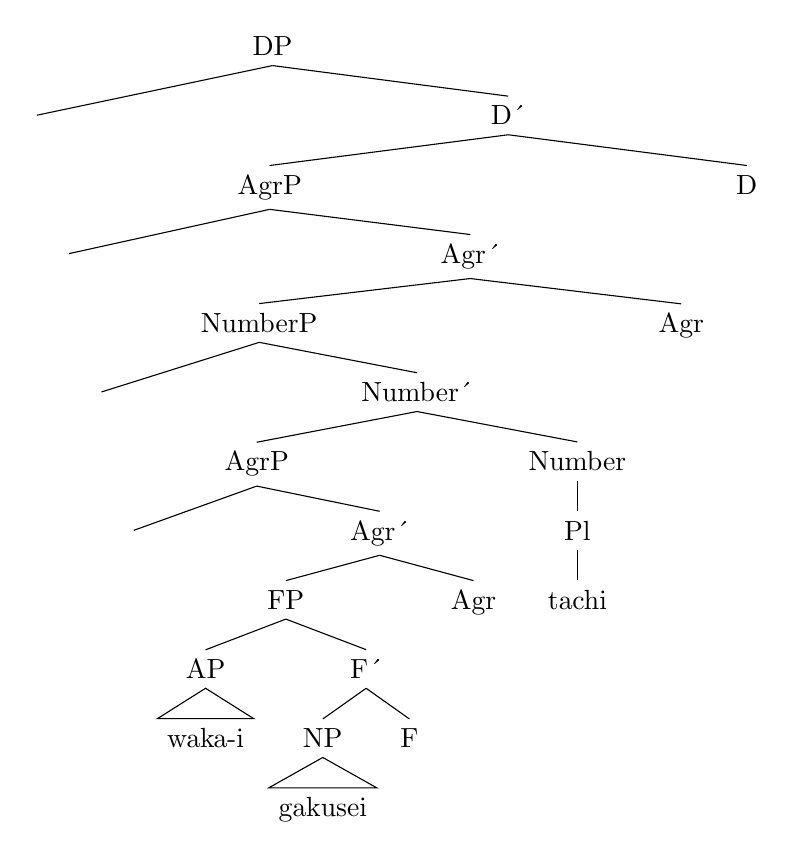
\begin{tikzpicture}[baseline=0pt, remember picture]
\tikzset{level distance=25pt, sibling distance=5pt}
 \Tree [.DP {} [.D´ [.AgrP {} [.Agr´ [.NumberP {} [.Number´ [.AgrP {} [.Agr´ [.FP [.AP \edge[roof]; waka-i ] [.F´ [.NP \edge[roof]; gakusei ] F ] ] Agr ] ] [.Number [.Pl tachi ] ] ] ] Agr ] ] D ] ]
\end{tikzpicture}

\section{Direct and indirect modification} \label{cartography Cinque}

In this section, I review the differences between direct and indirect modifiers, first, in order to derive reliable diagnostics for the type of modification, second, to relate their different structural positions to these diagnostics. In the following two sections, I elaborate on direct-only modifiers and the derivation of indirect modifiers. Discussions will be kept short here as they will be picked up in the following chapters.

\subsection{Introduction}

The notions \textit{indirect} and \textit{direct modification} were established by \citet{sproat:1991:the}. The authors used them as an explanation adjectives in Mandarin Chinese are ordered rigidly in some instances, but not in others. Precisely, they noted that an overt exponent of indirect modification is the element \textsc{de} 的 \citep[sec. 2]{sproat:1991:the}.\footnote{Analyzing the precise nature of \textsc{de} has been the task for a long time in syntactic research. \citet{sproat:1991:the} analyze it as a complementizer (see also \citealt{gobbo:2010:on}), but authors including Cinque (\citeyear{cinque:2010:adj}) do not share this proposal and have shown that some direct modifiers in fact have to appear with this element, (cf. \citealt{paul:2005:adj, paul:2010:adj, paul:2012:why, yang:2005:plurality}) and analyze it as `phrasal modifier'. Other analyses include `case assigner' \citep{larson:2009:chinese} or `linker' \citep{dikken:2004:complex}. \label{demandarin}} This element is optional in adjectival modification, but when it appears, it causes the absence of otherwise attested ordering restrictions, which are otherwise similar to the English case \citep[579]{sproat:1991:the}. This is shown below. %\is{adjective ordering restrictions}

\ex. \textsc{size} $\succ$ \textsc{color} without \textsc{de}
\ag. xi\v{a}o lù huāpíng\\
small green vase\\
\bg. ?lù xia\v{o} huāpíng\\
green small vase\\
`small green vase’ \null \hfill \citep[566]{sproat:1991:the}

\ex. \label{mandarin with de} \textsc{size} vs. \textsc{color} with \textsc{de}
\ag. xi\v{a}o de lù de huāpíng\\
small \textsc{de} green \textsc{de} vase\\
\bg. lù de xi\v{a}o de huāpíng\\
green \textsc{de} small \textsc{de} vase\\

Furthermore, this element is mandatory in verbal modification, which arguably always involves a relative clause structure. %\is{indirect modification}

\exg. [nèizhī jiào *(de)] g\v{o}u\\
that bark \textsc{de} dog\\
`the dog which is barking' \null \hfill \citep[573]{sproat:1991:the}

As mentioned above, cartography predicts that direct adjectives are merged in the specifier positions of functional heads that match their semantics and which are rigidly ordered. And since FP\textsubscript{SIZE} structurally dominates FP\textsubscript{COLOR}, linear adjacency is expected in context-neutral utterances. The hierarchical structure is depicted below for English \citep[28–30]{cinque:2010:adj}.\footnote{The threshold between the direct and the indirect domain is the indefinite head d. See Chapter \ref{indefinitedpdiscussion}.}

\newpage

\ex. \a. small green vase
\b. ??green small vase
\c. 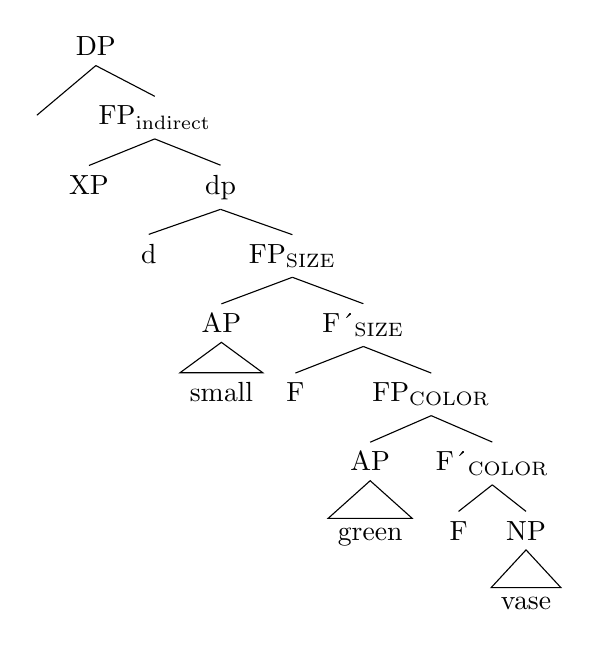
\begin{tikzpicture}[baseline=0pt, remember picture]
\tikzset{level distance=25pt, sibling distance=5pt}
\Tree [.DP {} [.FP\textsubscript{indirect} XP [.dp d [.FP\textsubscript{SIZE} [.AP \edge[roof]; {small} ] [.F´\textsubscript{SIZE} F [.FP\textsubscript{COLOR} [.AP \edge[roof]; {green} ] [.F´\textsubscript{COLOR} F [.NP \edge[roof]; \node (voitures4) {vase}; ]]]]]]]]]
\end{tikzpicture}

Indirect modifiers, on the other hand, are merged in the projection of relative clauses and since these functional projections are unordered with respect to semantic category, it is expected that indirect modifiers exhibit free order on the surface. This is what is at stake in Mandarin in \ref{mandarin with de}, claimed \citet{sproat:1991:the}, and this behavior is also observable in English (\citealt{baker:2003:verbal}).\footnote{Speakers might disagree on the possibility of relative clause stacking. And while \ref{bigredrc} does sound a bit stilted and was chosen mostly for the parallelism to the Mandarin example, same as the German example in \ref{bigredrcgerman}, examples of stacked relative clauses can be found, although preferably with longer relative clauses such as ``\textit{a book [that I wanted to read for a long time] [that was recommended to me by my teacher]}".}

\ex. \label{bigredrc} \a. a vase that is small that is green
\b. a vase that is green that is small

\subsection{Reduced relative clauses and ambiguities} \label{ambiguities}

Now, as mentioned in the introduction, most adjectives in English are actually ambiguous between a direct and an indirect status. Direct modifiers, here called \textit{direct-only}, are a very rare species. In fact, all adjectives that can have access to predicative use can have an indirect status when they appear in a simple modification structure. They are then not embedded under a full (also: finite) relative clause, but are instances of so-called \textit{reduced relative clause} (RRC) (\citealt[54–55]{cinque:2010:adj}, \citealt{douglas:2016:syntactic, harwood:2018:rrc}), relative clauses which lack a relative pronoun/a complementizer and a verb/a copula. This fact has also been put forth to explain deviations from expected ordering restrictions. If two indirect adjectives modify a noun, no fixed order is predicted, and languages where adjectives never follow ordering restrictions are predicted to only have indirect modification adjectives (cf. \citealt[ch. 3.3.2]{cinque:2010:adj}).

Verbal reduced relative clauses are easily recognizable in English, namely by virtue of lacking relative pronouns and copula, as for instance is the case with participle and infinitival relative clauses \citep{kayne:1994:anti, cinque:2020:relcl}, but there are also clear cases of indirect adjectives embedded in reduced relative clauses. Prototypical examples are postnominal adjectives of the type \textit{the man proud of his children} \citep{williams:1982:fofc, kayne:1994:anti, sadler:1994:prenominal, larson:2000:acd, larson:2004:indefinite}. While most adjectives in English are only licit in this position when they occur with complements or adjuncts,\footnote{The \textit{Head-Final Filter} of \citet{williams:1982:fofc}, cf. \citet{alexeyenko:2021:hff, richards:2022:finding, richards:2023:finding}.} there are some adjectives that can appear independently in this position, in addition to the prenominal position. Those include adjectives with the ending -\textit{ible/able} as in the following famous example from \citet[3--4]{bolinger:1967:adj}.\footnote{Adjectives with the initial prefix \textit{a}- such as \textit{afraid} or \textit{asleep} predominantly occur in postnominal position (\citealt{bolinger:1967:adj, larson:1998:events, larson:2004:indefinite}; \citealt[295]{alex:2007:nounphrase}; \citealt[ch. 2.3]{belk:2017:attributes}).} %\is{reduced relative clause}

\ex. \a. the (only) visible stars
\b. the (only) stars visible

It is well-known that such minimal pairs in English exhibit a meaning difference. In postnominal position, the adjectives denote a temporary, passing property, dubbed \textit{stage-level} reading. In prenominal position, they are ambiguous and can have this reading but additionally can also be understood as denoting an enduring property dubbed \textit{individual-level} reading (see \citealt{sadler:1994:prenominal, larson:1998:events, larson:2004:indefinite} and especially \citealt[Chapter 2.1]{cinque:2010:adj}). This allows the following paraphrases. %\is{subsective modifiers}

\ex. \a. the (only) stars visible $\approx$ `the only stars visible at the moment/that happen to be visible' (stage-level)
\b. the (only) visible stars $\approx$ `the only stars visible at the moment/that happen to be visible' (stage-level) OR `the only stars visible in general' (individual-level)

There are many such minimal pairs in English. What is common to each of them is that it is always the prenominal variant that is ambiguous, while the postnominal variant is restricted to a certain reading as shown below for the famous case of \textit{beautiful dancer} which can either have an intersective or a non-intersective reading (\citealt{larson:2000:acd, vendler:1957:verbs, siegel:1976:capturing, larson:1995:olga}). %\is{intersective modifiers}

\ex. \label{ambiguous, beautiful} Non-Intersective vs. Intersective \citep[145]{larson:1995:olga}
\a. Olga is a beautiful dancer. (ambiguous) \label{olga}
\b. $\approx$ `Olga is a dancer that dances beautifully.’ (non-intersective reading)
\c. $\approx$ `Olga is a dancer and Olga is beautiful.’ (intersective reading)

\ex. Non-Intersective vs. Intersective \citep[9]{cinque:2010:adj}
\a. Olga is a dancer more beautiful than her instructor. (only intersective)
\b. $\neq$ `Olga is a dancer that dances beautifully.’ (non-intersective reading)
\c. $\approx$ `Olga is a dancer and Olga is beautiful.’ (intersective reading) \label{intersective, RC}

Cartography offers an explanation for this: The ambiguity in interpretation observed in prenominal position arises since the adjective is syntactically ambiguous - it could be either direct or indirect. On the other hand, in postnominal position, the adjective can only be indirect. This can be verified when embedding it in a full relative clause. Again, only one reading is available: The same as int the postnominal use. This confirms that postnominal adjectives in English are predicative in nature \citep[18–19]{cinque:2010:adj}. %\is{direct modification}

\ex. Non-Intersective vs. Intersective, full RC \citep[9]{cinque:2010:adj}
\a. Olga is a dancer who is beautiful. (only intersective)
\b. $\neq$ `Olga is a dancer that dances beautifully.’ (non-intersective reading)
\c. $\approx$ `Olga is a dancer and Olga is beautiful.’ (intersective reading)

As a consequence, the reading not accessible in postnominal position, and not derived from predicative use, must be the direct reading and when adjectives such as \textit{beautiful} exhibit that reading, they must be interpreted as direct.

\subsection{Direct-only modifiers}

There is a small group of adjectives that are unambiguously direct. Those are called \textit{direct-only} in this book. According to \citet[ch. 4.1]{cinque:2010:adj}, these modifiers is \textit{functional} and \textit{phrasal}. They are functional because they arguably form a closed class, in most languages only with a couple of members \citep[43–44]{cinque:2010:adj}, explaining many cross-linguistic intersections. They are phrasal because they can appear with complements and have a phrasal character in some languages \citep[44–49]{cinque:2010:adj}. Below, I will review some well-known members as well as characteristics, but it should be kept in mind that both are, most of all, prototypical. %\is{direct-only modifiers}

A well-known group of direct-only modifiers are \textit{non-intersective}, also called \textit{intensional}, adjectives \citep{kamp:1995:prototype, panayidou:2013:in}, such as \textit{former}. Their inability to appear in predicative position, and thus also inside a relative clause, has been used to refute earlier transformational accounts à la \citet{smith:1964:det} and is a key diagnostic for direct-only status .

\ex. \a. a former president
\b. *This president is former.
\c. *a president who is former

In contrast to the \textit{beautiful dancer} example above, such adjectives only yield a non-intersective interpretation, also in attributive position, and are not ambiguous. %\is{non-intersective modifiers}

%\newpage

\ex. \a. Marya is a former dancer. (only non-intersective)
\b. $\approx$ `Marya was formerly a dancer.’ (non-intersective reading)
\c. $\neq$ `Marya is former, and Marya is a dancer.’ (intersective reading) \\ \null\hfill \citep[304]{alex:2007:nounphrase}

Further typical characteristics of direct-only modifiers include the inability to co-occur with degree expressions (Chapter \ref{gradability}) and to exhibit overt tense (Chapter \ref{test tense}). %\is{idiomatic modifiers}

\ex. *the very former president

\ex. *the (once) (was) former president / president who was former

Another type of direct-only modifiers are those that occur in idiomatic expressions. Those naturally diverge across languages. Modifiers participating in such constructions must occur prenominally in English. They can neither occur postnominally, nor in predicative position and still keep their idiomatic meaning \citep[ch. 7.2]{cinque:2010:adj}. %\is{idiomatic modifiers}

\ex. \a. a white lie \hfill \citep[88]{cinque:2010:adj}
\b. *a lie white (in spirit)
\c. *a lie (that) is white

\subsection{Linear distance}

Indirect modifiers are structurally higher than indirect modifiers, which predicts linear adjacency of direct modifiers to the noun. When an ambiguous modifier occurs twice in prenominal position in English, it does so once with each reading \citep[19–20]{cinque:2010:adj}. Although the intuition is subtle, it seems to be confirmed that the modifier closer to the noun has the direct reading as shown in \ref{visiblevisible} (cf. \citealt[280–281]{larson:2004:indefinite}).

\exg. The visible visible stars include Capella. \hfill \citep[155]{larson:1998:events}\\
the stage-level individual-level stars\\ \label{visiblevisible}

The two modifiers can also be spread out on both sides of the noun. Then, as expected, the postnominal modifier must bear the indirect modification, the stage-level reading \citep[19–20]{cinque:2010:adj}.

\exg. The visible stars visible include Capella. \null\hfill \citep[155]{larson:1998:events}\\
the individual-level stars stage-level\\

These observations hold for the other dichotomies, for example the intersective/non-intersective case.

\ex. \ag. Olga is a beautiful beautiful dancer.\\
Olga is a intersective non-intersective dancer\\
\null \hfill \citep[281]{larson:2004:indefinite}
\bg. Olga is a beautiful dancer more beautiful than her instructor.\\
Olga is a non-intersective dancer more intersective\\
\null \hfill \citep[19]{cinque:2010:adj}

\subsection{More on ordering restrictions} \label{AORs}

Standard cartography explains ordering restrictions among direct modifiers as a result of the distinct positions of the respective functional heads in the direct domain. Several hierarchies of functional heads for direct modification have been proposed, but a standard hierarchy for object nouns could look as follows. I have chosen the label \textsc{dimension} as a more broad term than \textsc{size}. It also includes the categories \textsc{length} and \textsc{width} from \citet[114]{scott:2002:stacked}.\footnote{Modifiers of \textit{action} or \textit{event} nouns \citep{grimshaw:1991:argument}, correspond to adverbs in the verbal domain \citep{cinque:1993:evidence, cinque:1999:adverbs, alexiadou:1997:adverb} and are often given in the following hierarchy: \textsc{speaker-oriented} $>$ \textsc{subject-oriented} $>$ \textsc{manner} $>$ \textsc{thematic} $>$ N \citep[324]{alex:2007:nounphrase}.} %\is{adjective ordering restrictions}

\ex. \textsc{quality} $>$ \textsc{dimension} $>$ \textsc{shape} $>$ \textsc{color} $>$ \textsc{nationality} $>$ \textsc{material} $>$ N \label{hierarchyjo}

Importantly, ordering restrictions are only maintained in \textit{hierarchical} modification. In \textit{parallel} modification, achieved via syndetic or asyndetic coordination, no ordering restrictions are expected \citep[578–580]{sproat:1991:the}.

\newpage

\ex. Parallel Modification (English)
\a. a red and big book \null \hfill syndetic
\b. a red, big book \null \hfill asyndetic

\subsection{Summary: Direct vs. indirect modifiers}

The defining characteristics that differentiate direct from indirect modifiers which offer valid diagnostics and tests to determine the status of a given modifier are summarized in the following table (cf. \citealt[33]{cinque:2010:adj} for a more detailed version).

\begin{center}
\begin{longtable}{|p{4cm}|p{4cm}|}
\hline
\textbf{Direct} & \textbf{Indirect} \\
\hline
\endfirsthead
\multicolumn{2}{c}
{\tablename\ \thetable\ -- \textit{Continued from previous page}} \\
\hline
\textbf{Direct} & \textbf{Indirect} \\
\hline
\endhead
\hline
\multicolumn{2}{c}{\textit{Continued on next page}} \\
\endfoot
\hline
\caption{Differences Between Direct and Indirect Modifiers}\\
\endlastfoot
Exhibit special readings, such as non-intersective, modal etc. & Exhibit the opposite readings: Intersective, implicit-RC etc. \\
\hline
Take part in idiomatic constructions & Only give literal interpretation \\
\hline
Impossible as predicates & Possible as predicates \\
\hline
Closer to the head noun & Further away from the head noun \\
\hline
Ordered rigidly & Show free/arbitrary ordering\\
\hline
Tend to be more simple & Are usually complex\\
\end{longtable}
\end{center}

\subsection{Cross-linguistic perspective}

It is an important enterprise of the cartographic research programs to verify those facts in cross-linguistic perspective. And indeed, they can, and often do, serve as valid diagnostics for modification status in other languages as well. A cartographic account of the DP has been proposed for French \citep{laenzlinger:2005:french, laenzlinger:2011:elements}, Greek (\citealt[appendix]{cinque:2010:adj}; \citealt{panayidou:2013:in}), Russian (\citealt{siegel:1976:capturing}; \citealt[appendix]{cinque:2010:adj}), Dutch \citep{belk:2017:attributes}, Korean \citep{kang:2005:adj, kang:2006:two, kim:2019:syntax}, Javanese \citep{vander:2009:direct} and Kipsigis \citep{kouneli:2019:syntax}.\footnote{See also the appendix of \citet{cinque:2010:adj} for Romanian, Maltese and German and the typological sample in \citet{laenzlinger:2010:cp, laenzlinger:2011:elements}.} That ordering restrictions, or at least tendencies, have cross-linguistic validity is exemplified for German in \ref{bigredgerman}. Again, once the modifiers are embedded in corresponding relative clauses, their order becomes free \ref{bigredrcgerman}. %\is{adjective ordering restrictions}

\ex. \label{bigredgerman} \textsc{size} vs. \textsc{color} (German)
\ag. ein großes rotes Buch\\
a big red book\\
\bg. ??ein rotes großes Buch\\
a red big book\\
`a big red book’

\ex. \label{bigredrcgerman} \textsc{size} vs. \textsc{color} indirect (German)
\ag. ein Buch, das groß ist, das rot ist\\
a book that big is that red is\\
\bg. ein Buch, das rot ist, das groß ist\\
a book that red is that big is\\
`a book which is big which is red’

The resolution of ambiguities also holds in Italian (Romance), where adjectives are freer in their distribution to the left and to the right of the noun. Ambiguous adjectives of the \textit{beautiful}-type show this ambiguity in their prototypical position as well, but this is the postnominal position \ref{italianattacantebuono}. On the contrary, in the, more marked, prenominal position, the relevant adjectives only have one interpretation. This interpretation is the opposite of the English postnominal cases, thus corresponds to the direct reading \ref{italianbuonoattacante}. From this, \citet[ch. 2.4]{cinque:2010:adj} concludes that prenominal adjectives in Italian must be direct (examples taken from \citealt[10]{cinque:2010:adj}). %\is{subsective modifiers, german}

\exg. Un \textbf{attaccante} \textbf{buono} non farebbe mai una cosa del genere.\\
a forward good \textsc{neg} would.do never a thing of.\textsc{det} sort\\
1.. $\approx$ `A forward good at playing forward would never do such a thing.’ (non-intersective)\\
2. $\approx$ `A good-hearted forward would never do such a thing.’ (intersective) \label{italianattacantebuono}

\exg. Un \textbf{buono} \textbf{attaccante} non farebbe mai una cosa del genere.\\
a good forward \textsc{neg} would.do never thing of.\textsc{det} sort\\
1. $\approx$ `A forward good at playing forward would never do such a thing.’ (non-intersective)\\
2. $\neq$ `A good-hearted forward would never do such a thing.’ (intersective) \label{italianbuonoattacante}

The same ambiguous adjective with two different readings is only possible postnominally. Nevertheless, the relative closeness is preserved: The adjective with the direct modification interpretation must be closer to the noun than the adjective with the indirect modification reading \citep[20–22]{cinque:2010:adj}. %\is{italian}

\exg. Un attaccante \textbf{buono} buono \\
a forward good(non-intersective) good-hearted(intersective)\\
`a good-hearted good forward' \null\hfill \citep[21]{cinque:2010:adj}

\section{Groups of direct-only modifiers} \label{directmodifiers}

This section presents the two biggest cross-linguistic groups of direct-only modifiers. Besides non-intersective modifiers, which were already looked at, I will discuss \textit{relational} modifiers. Both these groups are relevant for the discussion of direct modifiers in Japanese in Chapter \ref{direct japanese}. %\is{direct-only modifiers}

\subsection{Non-intersective modifiers} \label{intersective}

\subsubsection{Truly non-intersective modifiers}

Non-intersective modifiers of the type \textit{former} or \textit{alleged} are characterized by the fact that they do not denote a set intersection with the noun they modify \citep{vendler:1957:verbs, siegel:1976:capturing, bolinger:1967:adj, kamp:1995:prototype, larson:1998:events}. This is illustrated with the English adjective \textit{former} below where there is no set intersection between the set of presidents and the set of former entities pertaining to Obama. %\is{direct-only modifiers, non-intersective modifiers}

\ex. \a. Obama is the/a former president.
\b. [former president] $\neq$ [former] $\cap$ [president]

As predicative use enforces the intersective reading, it is only logical that these modifiers cannot be used predicatively.

\ex. *This president is former.

Such \textit{truly non-intersective} modifiers often refer to a time (former, future, present), a place (\textit{dortig}; German: `over there’) or a manner (possible, main), highlighting their connection to adverbs. This group has also been recognized in Japanese \citep{yamakido:2005:nature, ayano:2010:revisiting} and behaves alike. Non-intersective modifiers in Japanese cannot be used predicatively and do not denote intersections with the noun.

\ex. \ag. Tarō-ga shōrai-no purosakkāsenshu-da.\\
Taro-\textsc{nom} future-\textsc{no} pro.soccer.player-\textsc{cop}\\
`Taro is a future professional soccer player.’
\bg. *Ano purosakkāsenshu-ga shōrai-da.\\
that pro.soccer.player-\textsc{nom} future-\textsc{cop}\\
(`That professional soccer player is future.’)
\c. [shōrai-no purosakkāsenshu] $\neq$ [shōrai] $\cap$ [purosakkāsenshu]

\subsubsection{Subsective modifiers}

Notably, there is an in-between-class of modifiers between intersective and non-intersective modifiers, usually called \textit{subsective}, where modifiers co-occur with nouns depicting an event or a profession and only modify part of the extension of those nouns. A well-known example is the following \citep[137–138]{kamp:1995:prototype}. %\is{direct-only modifiers, subsective}

\ex. Mary is a skillful surgeon.

The most salient interpretation of this phrase is that Mary is skillful as a surgeon, so she is experienced in her profession of operating people. The interpretation `Mary is skillful.’ again seems not really available, because we do not know what she could be skillful at. Subsective modifiers are able to appear in predicative position and thus also in relative clauses, but then, only one interpretation remains, namely the intersective one. The subsective interpretation, on the other hand, is inaccessible.

\ex. \a. Mary is a surgeon who is skillful. (only intersective)
\b. $\neq$ `Mary is skilfull as a surgeon.’ (subsective)
\c. $\approx$ `Mary is a surgeon and Mary is skillful.’ (intersective)

Subsectivity is the source of most ambiguities mentioned above, including the famous \textit{beautiful dancer} example (\citealt[145]{larson:1995:olga}; \citealt{vendler:1957:verbs, siegel:1976:capturing}). The paraphrase `beautiful as a dancer’ is in fact the subsective, while the paraphrase `beautiful and a dancer’ is the intersective reading.

\ex. \a. Olga is a beautiful dancer.
\b. [beautiful dancer] $\subseteq$ [dancer] (subsective)
\c. [beautiful dancer] = [beautiful] $\cap$ [dancer] (intersective)

Another well-known ambiguous example is the following.

\ex. \a. Peter is an old friend. \hfill \citep[146]{larson:1998:events}
\b. [old friend] $\subseteq$ [friend] (subsective: `long-time friend’)
\c. [old friend] = [old] $\cap$ [friend] (intersective: `aged friend’)

In Chapter \Ref{non-intersective Japanese}, it will be shown that Japanese nominal modification does not readily allow such ambiguities, one reason why direct modification has been denied. Instead, ambiguities are resolved via different lexemes, each exhibiting an intersective and a non-intersective reading.

\subsubsection{Privative modifiers}

Another group of non-intersective modifiers are privative modifiers. Such modifiers, often similar in spirit to the meaning `fake’, denote a zero intersection with their head noun. %\is{direct-only modifiers, privative modifiers}

\ex. \a. a fake gun
\b. [fake gun] $\cap$ [gun] = $\emptyset$ \hfill \citep[25]{morzycki:2016:mod}

Interestingly, such modifiers can appear in predicative position, which is why \citet{partee:2009:formal} has proposed that privative adjectives in English and Russian might be subsective after all, therefore not direct-only.

\ex. This gun is fake / pretend / artificial. \hfill \citep[25]{morzycki:2016:mod}

This is also the case in Japanese where predicative use of the privative modifier \textit{nise-no} `fake' is degraded, but not entirely ungrammatical.

\exg. ?Kono pisutoru-wa nise-da.\\
this gun-\textsc{top} fake-\textsc{cop}\\
`This gun is fake.'

As shown in \citet[21–23]{cinque:2014:semantics} however, there is reason to analyze privative modifiers as direct-only. Consider the following minimal pair with the Italian equivalent \textit{falso} `false’.

\ex. \ag. le false banconote\\
\textsc{det} fake bank.note.\textsc{pl}\\
only: `Monopoly money’
 \bg. le banconote false \\
\textsc{det} bank.note.\textsc{pl} fake\\
only: `counterfeited money’ \hfill \citep[21]{cinque:2014:semantics}

In prenominal position -- remember the position only having a direct modifier reading in Italian -- \textit{falso} has a reading as `\textit{Monopoly money}’, whereas in postnominal position it only has a reading as `\textit{forged/counterfeited money}’. As expected, this reading corresponds to the reading in predicative position.

\exg. Quelle banconote sono false.\\
this bank.note.\textsc{pl} are fake\\
1. $\approx$ `This money is counterfeited.’\\
2. $\neq$ `This money is Monopoly money.’ \null\hfill \citep[21]{cinque:2014:semantics}

\subsubsection{Adnominal degree modifiers}

A final group is what \citet{morzycki:2016:mod} calls \textit{adnominal degree modifiers}. %\is{direct-only modifiers, adnominal degree modifiers}

\ex. He is a complete / total / utter / absolute / true idiot. \\ \null\hfill \citep[56–57]{morzycki:2016:mod}

As the name suggests, \citet{morzycki:2014:where, morzycki:2016:mod} does not see these elements as lexical adjectives, but rather as functional modifiers that denote a (often, but not always extreme) point on a scale for certain nouns. Nevertheless, they are relevant for this study since they cannot be used predicatively.

\ex. *This idiot is complete / total / utter / absolute / true.

\subsection{Relational adjectives} \label{RA}

\subsubsection{Nominal derivation and syntactic constraints}

\textit{Relational adjectives}, such as \textit{environmental} or \textit{technical}, make up a relatively rich research field. They have been discussed predominantly with regard to Romance languages and English, but also in Japanese \citep{bisetto:2010:RA, nagano:2015:RA, nagano:2016:are, nagano:2018:conversion, shimada:2018:relational, morita:2010:internal, morita:2011:three, morita:2013:morph} and will be picked up in Chapter \Ref{RAJapanese}. Morphologically, they are characterized via their denominal appearance, exhibiting typical suffixes such as -\textit{al}, \textit{ic(al)} in English or -\textit{ar}, -\textit{lich} or -\textit{isch} in German. This oftentimes gives relational adjectives a scientific flavor (cf. \citealt{gunkel:2008:constraints}).\footnote{They are therefore also sometimes called ``denominal adjectives’’ or ``(denominal) pseudo-adjectives’’ \citep{postal:1969:anaphoric, bartning:1980:remarques}. See \citet[52–56]{bortolotto:2016:RA} for an overview.} Semantically, they denote a specific relationship to the nouns they modify and do not just simply add a quality, as would ordinary \textit{qualitative} adjectives. Syntactically, the following cross-linguistic characteristics of relational adjectives have been established.\footnote{For English and Romance see \citet{postal:1969:anaphoric, downing:1977:creation, levi:1978:syntax, bartning:1980:remarques, bartning:1984:aspects, bartning:1986:paralelisme, warren:1984:classifying, bosque:1993:sobre, bosque:1996:postnominal, mcnally:2004:relational, fabregas:2007:internal, fabregas:2014:adjectival, gunkel:2008:constraints, roy:2010:deadjectival, zifonun:2011:RA, rainer:2013:can, bortolotto:2016:RA}, and for an overview \citet[Chapters 3.3 and 9.2]{alex:2007:nounphrase}. They have also been discussed in German \citep{hotzen:1967:gegenwart, schaublin:1972:probleme, eichinger:1979:syntaktische, frevel:2005:RA, trost:2006:das}, Russian \citep{mezhevich:2002:english}, Polish \citep{cetnarowska:2015:categorial}, Hungarian \citep{kenesei:2014:on} and Selkup \citep{spencer:2017:denominal, nikolaeva:2020:mixed}. See \citet[44]{nagano:2016:are} or \citet[ch. 2.3]{bortolotto:2016:RA} for similar overviews.} %\is{direct-only modifiers, relational modifiers}

\ex. Characteristics of relational adjectives
\a. They cannot be used predicatively. (*this crisis is environmental)
\b. They are not gradable. (*more/most environmental crisis; *very environmental crisis)
\c. They have to be strictly adjacent to their head noun and cannot be combined with regular qualitative adjectives. (*environmental huge crisis; *huge and environmental crisis; *environmental and huge crisis)
\d. They appear in certain positions from which they cannot move, typically they occur in postnominal position in Romance languages. (*\textit{chimico processo}; \textit{processo chimico} `chemical process', Italian; \citealt[59]{bortolotto:2016:RA})
\e. They cannot be nominalized. (*environmental-ity)
\f. They lack polarity/do not come in antonym pairs. (*un-environmental; *non-environmental)

The fact that they cannot be used predicatively defines them as direct modifiers as tested in many different languages. %\is{direct-only modifiers, relational modifiers}

%\newpage

\ex. \a. *My appointment this afternoon is dental. (English) \null \hfill \citep[49]{rae:2010:ordering}
\b. *This linguist is theoretical.

\exg. *Dieser Linguist ist theoretisch. (German)\\
this linguist is theoretical \\

\exg. *L’élection est présidentielle. (French)\\
\textsc{det}.election is presidential \\\null \hfill \citep[68]{bortolotto:2016:RA}

\exg. *Magazin byl kni\v{z}-n-yj. (Russian)\\
store was book-\textsc{ra-nom.sg.m} \\ \null \hfill \citep[100]{mezhevich:2002:english}

Importantly, relational adjectives can occur in predicative position in certain circumstances. One involves the class shift into a qualitative adjective (cf. \citealt{nagano:2018:conversion}). %\is{German, English, French, Russian}

\ex. The way he approached this problem was very theoretical.

This shift can be facilitated by degree adverbs such as \textit{very} as in \ref{italian party}. The \textit{ethnic} adjective \textit{Italian} (\citealt{alex:2011:ea}, see below) has acquired a qualitative meaning as shown by the available paraphrases.

\ex. \label{italian party} \a. The party yesterday was very Italian.
\b. $\neq$ `The party took place in Italy, was organized by Italians, etc.’ (relational reading)
\c. $\approx$ `The party featured many Italian dishes, music, etc.’ (qualitative reading)

Another way in which relational adjectives can be used predicatively is when they have a \textit{kind-reading} \citep{mcnally:2004:relational} as in the following example from Catalan. This example can essentially be paraphrased by \textit{this tuberculosis can be of the pulmonary kind/type}, and from a syntactic point of view allows the recovery of a noun \textit{kind} or \textit{type}. %\is{Catalan}

%\newpage

\exg. La tuberculosi pot ser pulmonar. (Catalan)\\
\textsc{det} tuberculosis can be pulmonary\\
`The tuberculosis could be pulmonary.’ \\ \null \hfill \citep[189]{mcnally:2004:relational}

Relational adjectives also resist gradability, at least with \textit{indefinite degree adverbs} \citep{fabregas:2014:adjectival} of the type \textit{very}. Many are however compatible with so-called \textit{modifiers of extension} (\citealt{fabregas:2014:adjectival}; called `\textit{endpoint-oriented modifiers}' in \citealt{kennedy:2005:scale}) such as \textit{completely} or \textit{100 percent}.

\ex. This is a *very / completely / 100 percent environmental problem.

Relational modifiers, as direct modifiers, are not only very low in the DP, they are also lower than many other direct modifiers, predicting strict adjacency to the noun. This holds cross-linguistically as shown for French below. Relational adjectives, such as \textit{industriel} `industrial’, obligatorily appears postnominally, and must be closer to the noun than qualitative adjectives, whatever status one assumes for them. %\is{french, relational modifiers}

\ex. \ag. un développement industriel rapide (French)\\
a development industrial rapid\\
`a fast industrial development’
\bg. *un développement rapide industriel\\
a development rapid industrial \null \hfill \citep[61]{bortolotto:2016:RA}\\

In Japanese, relational adjectives have been identified amongst the group of \textit{no}-modifiers, free of morphological processes (\citealt{bisetto:2010:RA, nagano:2016:are} a.o.). Importantly they do fulfill the relevant characteristics, a restriction on predicativity and gradability.

\ex. \ag. kankyō-no kiki \\
environment-\textsc{no} crisis\\
`environmental crisis’
\bg. *Kono kiki-ga kankyō-da.\\
this crisis-\textsc{nom} environment-\textsc{cop}\\
(`This crisis is environmental.’)
\cg. *totemo kankyō-no kiki \\
very environment-\textsc{no} crisis\\
(`very environmental crisis’)

This suggests that those lexemes are simply nouns, since no obvious derivational patterns are detectable. Furthermore, relational adjectives in this language do not compete with other constructions, such as compounds or PPs with the same meaning, which is very well observed in European languages (for example \textit{nominal modification} vs. \textit{noun modification} in English, \citealt{hacken:2013:compounds, rainer:2013:can, nikolaeva:2020:mixed}). Again, Japanese has only one option of modification at its disposal where other languages can show variation.

\subsubsection{Classificatory, thematic and ethnic adjectives}

While in many cases, relational adjectives, classifies the type of noun they modify, they can also express argument status. This happens when they modify event or action nouns \citep{grimshaw:1991:argument}.

\ex. environmental protection

Here, \textit{environmental} expresses the role of the internal argument of the verb \textit{to protect} underlying the action noun.\footnote{Theoretically, it could express a subject role, but our world knowledge tells us that the environment needs to be protected, rather than is the protecter.} Relational adjectives used this way have been called \textit{thematic} since they ``saturate semantic roles“ \citep[360]{bosque:1996:postnominal} contrasting them with \textit{classificatory relational adjectives}. Thematic relational adjectives are interesting since cross-linguistic variation in the type of argument they can express has been detected. For instance, in German, object readings of thematic adjectives are categorically impossible \citep{gunkel:2008:constraints}. %\is{direct-only modifiers, thematic modifiers}

\exg. städt-isch-e Reinigung (German)\\
city-\textsc{ra-nom.f.sg} cleaning.\textsc{nom.f.sg}\\
1. $\approx$ `cleaning by the city' (subject) \\
2. $\neq$ `cleaning of the city' (object) \\ \null \hfill \citep[294]{gunkel:2008:constraints}

Another relevant subgroup are so-called \textit{ethnic adjectives}. Ethnic adjectives are toponymic modifiers which denote a geographical origin and sometimes even titles and can be thematic or classificatory \citep{giorgi:1991:syntax, alex:2011:ea, arseni:2014:EA, kotowski:2016:adj}. Arguably, they also show restrictions in their use as thematic modifiers, resisting the role of direct objects. This goes back to the following classic example of \citet[111]{kayne:1981:ecp}.

\ex. \a. Everyone deplored the Russian destruction of China. (Subject reading)
\b. *Everyone deplored the Chinese destruction by Russia. (Object reading)

On the other hand, the \textsc{theme} reading is possible in English with genitive modifiers \citep{kayne:1981:ecp}.

\ex. Everyone deplored China's destruction by Russia. (Object reading)

Classificatory ethnic adjectives exist as well. As they correspond to the categories \textsc{nationality}/\textsc{origin}/\textsc{provenance} put forth in \citet{sproat:1991:the, scott:2002:stacked, laenzlinger:2005:french, cinque:2010:adj}, they are often not treated as true ethnic adjectives. Importantly, contrary to relational adjectives, these adjectives can, at least in some languages, appear in predicative position, including English \ref{ethnic english} and Greek \ref{ethnic greek}.

\ex. These bed sheets are Italian. \label{ethnic english}

\exg. I tsanta tis ine italiki. (Greek)\\
\textsc{det} bag \textsc{poss.3.sg} \textsc{cop} Italian\\
`Her bag is Italian.' \null \hfill \citep[138]{alex:2011:ea} \label{ethnic greek}

In Japanese, modifiers that express \textsc{nationality} only appear among the group of \textit{no}-modifiers and can never be used predicatively, neither with object nor with event nouns. This highlights their status as direct-only modifiers. %\is{direct-only modifiers, classificatory modifiers, ethnic modifiers, Greek}

\ex. \ag. *Kono kuruma-wa Nihon-da. \label{nihon}\\
this car-\textsc{top} Japan-\textsc{cop}\\
(`This car is Japanese.’)
\bg. *Kono kōgeki-wa Nihon-da.\\
this car-\textsc{top} Japan-\textsc{cop}\\
(`This attack is Japanese.’)

\subsubsection{Categories and ordering} \label{ordering relational}

Relational adjectives also show ordering restrictions among each other analyzed in \citet{bortolotto:2016:RA} for many Romance languages.

\ex. \ag. escursioni montane estive (Italian)\\
hike.\textsc{pl} mountain.\textsc{ra.pl}. summer.\textsc{ra.pl}\\
\bg. ??escursioni estive montane\\
hike.\textsc{pl} summer.\textsc{ra.pl} mountain.\textsc{ra.pl}\\
`mountain summer hikes’ \null\hfill \citep[148]{bortolotto:2016:RA}

The systematic hierarchy established in \citet{bortolotto:2016:RA} reads as follows. %\is{adjective ordering restrictions}

\ex. \emph{Hierarchy of Relational Adjectives (based on \citealt[180]{bortolotto:2016:RA}})\\
\textsc{time} $>$ \textsc{location} $>$ \textsc{agent} $>$ \textsc{instrument} $>$ \textsc{matter} ($>$) \textsc{theme} $>$ N

\subsection{Summary}

Both, non-intersective as well as relational modifiers are thus groups of modifiers, whose existence in Japanese immediately verifies the existence of direct modification.

\section{Indirect modification} \label{dP}

This section outlines the two types of indirect modifiers and briefly discusses the syntax of indirect modifiers focusing on the derivation adopted in this book. Indirect modification will be the topic of Chapter \ref{indirect japanese}.

\subsection{Two kinds of indirect modifiers: Full vs. reduced relative clauses} \label{chapter RC}

\subsubsection{General differences}

As mentioned above, indirect modifiers come in two types: \textit{Full relative clauses} and \textit{reduced relative clauses} (RRCs) \citep{cinque:2010:adj, cinque:2020:relcl, krause:2001:rrc, douglas:2016:syntactic, harwood:2018:rrc}. Traditionally, reduced relative clauses have been assumed to be derived from full relative clauses \citep{smith:1964:det} and the following characteristics are often invoked that highlight their reduced/impoverished nature (\citealt[203]{cinque:2020:relcl}; \citealt{bhatt:1999:covert, krause:2001:rrc, douglas:2016:syntactic, harwood:2018:rrc}). %\is{indirect modifiers}

\ex. Characteristics that differentiate reduced from full relative clauses \label{chara rrc}
\a. They do not make use of relative pronouns or complementizers.
\b. Fewer positions on the Accessibility Hierarchy \citep{keenan:1977:noun} can be relativized/only the subject can be relativized.
\c. Tense is reduced/No tense is involved.
\d. No overt subject appears.
\e. A restriction to certain types of verbs applies.

These characteristics seem accurate in languages such as English, although the problem arises to differentiate reduced relative clauses from adjectives, if they do not appear postnominally or are participial or infinitival. Testing the status of a relative clause in a prenominal-RC language,\footnote{With this notion I refer to languages with only prenominal relative clauses in line with \citet{wu:2011:syntax}.} however, is almost impossible to test based on these criteria alone. That is mainly because in such languages, usually only one surface form for relative clauses exists and relative pronouns/complementizers are typically absent. While these facts speak for a reduced status, the fact that overt subjects typically appear freely and many positions on the Accessibility Hierarchy can be relativized speak for a larger status (cf. \citealt{wu:2011:syntax}). %\is{reduced relative clauses}

In the cartographic program, two structural differences have been identified for full and reduced relative clauses: 1. The internal make-up of reduced relative clauses contains less functional material. 2. They occupy different merging positions.

Regarding the first point, while full relative clauses are of the structural size CP, reduced relative clauses are (arguably) smaller, although their exact size is controversial. In seemingly well-known languages such as English, convincing evidence, mostly in the form of co-occurrence with high adverbials \citep{douglas:2016:syntactic, harwood:2018:rrc, cinque:2020:relcl} can be found that they must be at least of size IP. On the other hand, some authors have argued that reduced relatives in prenominal-RC languages are only vPs \citep{krause:2001:rrc}, while some assume a specific PrtP projection for participles \citep{bhatt:1999:covert}.

\subsubsection{Ordering and the syntax of the indirect domain}

Ordering restrictions, arguably, provide a better testing ground. According to \citet{cinque:2010:adj, cinque:2020:relcl}, the indirect domain (the area up to dP, see below) looks as depicted in the (simplified) tree below.

\ex. \begin{tikzpicture}[baseline=0pt, remember picture]
\tikzset{level distance=25pt, sibling distance=1pt}
 \Tree [.DP {} [.FP\textsubscript{RC} CP [.F´\textsubscript{RC} F [.FP\textsubscript{Num} NumP [.FP\textsubscript{RRC} IP [.F´\textsubscript{RRC} F [.dP d [.FP\textsubscript{direct} {} [.... {} [.NP \edge[roof]; \node (NP) {N}; ] ] ]]] ]]]] ]
 \end{tikzpicture}

Within the indirect domain, the projections for full relative clauses are higher than the projections for reduced relative clauses. Recall that several projection for the same type have to be assumed, explaining cases of relative clause stacking. Furthermore, there is a projection for numerals intervening. This predicts the following overall hierarchy. %\is{indirect modifiers, reduced relative clauses}

\ex. (\textsc{demonstrative}) ($>$) \textsc{relative clause} $>$ \textsc{numeral} $>$ \textsc{reduced relative clause} ($>$) (dP) ($>$) (\textsc{direct adjective}) ($>$) (N)

In fact, the interaction with numerals serves as an important test bed as well: Full relative clauses cross-linguistically typically linearly precede numerals, while reduced relative clauses follow them, in languages where they are on the same side of the noun. That full relative clauses typically precede numerals has been identified already in \citet{greenberg:1963:some} and \citet{hawkins:1983:word} and is further discussed in \citet{cinque:2005:deriving, cinque:2023:linearization}.\footnote{Similarly, relative clauses precede adjectives, see \citet{cinque:2005:deriving, cinque:2023:linearization}; \citet[298–299]{rijkhoff:2002:noun}.} In those rigid head-final and head-initial languages which exhibit a more or less homomorphic order of constituents, this is what is observable \citep[ch. 3.5]{cinque:2020:relcl} as illustrated in the examples below, which provide evidence for the hierarchy \textit{demonstrative} $>$ \textit{relative clause} $>$ \textit{numeral} (cf. \citealt[225]{cinque:2020:relcl}).

\exg. [he taa-w kuttuwa ehida] iccashu adussa laagge-t-i\\
those I-\textsc{dat} chicken having.brought five tall friend-\textsc{pl-nom}\\
`those five tall friends [who brought me a chicken]’ \\ \null \hfill Wolaytta, West Cushitic, head-final (\citealt[215]{lamberti:1997:wolyatta})

\exg. gwóggî à dòŋò àryó-nì [ámê lóc\textschwa {} ònèkò]-nì \\
dogs \textsc{att.part} big two-this \textsc{rel} man \textsc{3.sg}.kill.\textsc{perf}-this\\
`these two big dogs [that the man killed]’ \\ \null \hfill Lango, Eastern Nilotic, head-initial (\citealt[156]{noonan:1992:lango})

On the other hand, the underlying order \textit{numeral} $\succ$ \textit{RRC} can be verified in German (\ref{numeral rrc german}; cf. also \citealt{eichinger:1991:ganz, trost:2006:das}) and English \ref{numeral rrc english}. Numerals and participle (reduced) relative clauses must both occur prenominally and are best in that order. %\is{indirect modifiers, German}

\ex. \label{numeral rrc german} \ag. die drei [dort parkenden]\textsubscript{RRC} Autos (German)\\
the three there parking.\textsc{prs.ptcp} cars\\
\bg. ??die [dort parkenden]\textsubscript{RRC} drei Autos\\
the there parking.\textsc{prs.ptcp} three cars\\
`the three cars parking over there’

\ex. \label{numeral rrc english} \a. these (other) two [recently completed]\textsubscript{RRC} plays
\b. ?these (other) [recently completed]\textsubscript{RRC} two plays \null \hfill \citep[229]{cinque:2020:relcl}

\subsubsection{A Note on the indefinite head dP} \label{indefinitedpdiscussion}

According to \citet{cinque:2010:adj, cinque:2020:relcl}, the threshold between the direct and the indirect domain is the indefinite head d, which is the ``head of the relative clause itself“ \citep[34]{cinque:2010:adj} and bears an identical constituent within the relative clause. The syntactic role of d as the \textit{external head} and counterpart to the \textit{internal head} is essentially relevant in Cinque’s theory on the double-headedness of relative clauses \citep{cinque:2020:relcl}. From a semantic point of view, d assigns ``referential import“ \citep[34]{cinque:2010:adj} meaning that modifiers above this head modify nouns with referentiality of their own. The author seems to have in mind a more referential status of relative clauses, which, for instance, matches the intersective interpretation, whereas direct modifiers not necessarily bear this feature of referentiality, which explains their non-intersective interpretation. In this book, dP will be displayed as the threshold between the two domains, but it does not serve a syntactic function beyond that, as the double-headed structure will not be adapted for Japanese. %\is{dP}

\subsection{The syntactic derivation of relative clauses}

\subsubsection{The underlying structure}

A plethora of different analyses can be found for the structure and derivation of (the different types of) relative clauses in English alone \citep{schachter:1973:focus, vergnaud:1974:french, vergnaud:1985:dep, kayne:1994:anti, bianchi:1999:consequences, bhatt:2002:raising, salzmann:2019:new}. What is common to them is that they must find a way to solve the \textit{connectivity problem} \citep{salzmann:2017:reconstruction}, i.e. the question how the correct interpretation of the noun, both inside the relative clause and inside the matrix clause, can be ascertained. Prior to derivation, I assume the underlying structure of a full relative clause to look as follows following cartographic research until \citet{cinque:2010:adj}. %\is{indirect modifiers, relative clause}

\newpage

\ex. \a. I read the book [that John wrote].
\b. \begin{tikzpicture}[baseline=0pt, remember picture]
\tikzset{level distance=25pt, sibling distance=1pt}
 \Tree [.DP the [.Agr \node (Agr) {}; [.Agr´ Agr [.FP\textsubscript{RC} [.CP {} [.C´ [.C that ] [.IP [.DP \edge[roof]; {John} ] [.I´ I [.VP {} [.V´ [.V write ] {} ] ] ] ]] ] [.F´\textsubscript{RC} F [.FP\textsubscript{Num} NumP [.FP\textsubscript{RRC} IP [.F´\textsubscript{RRC} F [.dP d [.FP\textsubscript{direct} {} [.... {} [.NP \edge[roof]; \node (NP) {book}; ] ] ]]] ]]]] ]]]
 \end{tikzpicture}

The relative clause is a full one, thus is of status CP. It merged in the specifier position of a corresponding projection for full relative clauses, which is higher than the projection for numerals and those for reduced relative clauses. The structure for a reduced relative clause looks similarly except for the fact that a CP-layer is lacking. %\is{numerals}

\subsubsection{The derivation}

Three major types of analyses have been invoked for head-external relative clauses, each of them ensuring in a different way that the noun can be interpreted correctly both inside the relative clause, where it is not present on the surface, and within the matrix clause:\footnote{Even among a single stream of analysis, several differences exist as to the fine details and technicalities of the derivation. I will simplify these details and differences in the following discussion. See \citet[ch. 2]{salzmann:2017:reconstruction} for an informative overview.}

\begin{enumerate}
\item The Raising Analysis
\item The Matching Analysis
\item Operator Movement
\end{enumerate}


In the raising analysis, also known as \textit{promotion} or \textit{head-internal} analysis, the noun is structurally present inside the relative clause at the beginning of the derivation. It then \textit{raises} out of the relative clause and leaves behind a trace. This guarantees the correct interpretation \citep{schachter:1973:focus, vergnaud:1974:french, vergnaud:1985:dep, kayne:1994:anti, bianchi:1999:consequences, bhatt:2002:raising}.

According to the \textit{matching} analysis, no movement happens. Instead, there are two instances of the noun, one inside and one outside the relative clause. The noun inside the relative clause (in some versions the complement of an operator) is deleted at PF under phonological identity with the noun in the matrix clause \citep{lees:1961:constituent, chomsky:1965:aspects, schachter:1973:focus, sauerland:1998:the, sauerland:2003:a, salzmann:2017:reconstruction, salzmann:2019:new}.

Both analyses have been proven to be valid in different languages. Essentially, the difference boils down to the fact that in raising analyses, movement of the noun takes place. This predicts the availability of different syntactic reconstruction effects, such as idiomatic readings and island effects (see \citealt{cinque:2008:more, cinque:2020:relcl, salzmann:2017:reconstruction, salzmann:2019:new} for overviews and discussions). %\is{indirect modifiers, relative clause}

In this book, I will adopt the standard, older and not uncontroversial, \textit{operator-movement} derivation for Japanese in Chapter \ref{operator}, according to which a relative clause operator moves from within the relative clause, for instance from the complement position of the verb in object relative clauses, to Spec, CP. This operator is co-indexed with the head noun outside the relative clause and ensures it is interpreted correctly inside the relative clause as well (cf. \citealt{chomsky:1977:on}, especially \citealt{miyamoto:2017:RC} for Japanese). This derivation is also given as a possible derivation for Japanese, and other prenominal relative clause languages in \citet[81]{cinque:2020:relcl}, abstracting away from the double-headed structure. For English, the structure looks as follows, including movement of the noun to a higher functional projection for word order purposes. %\is{indirect modifiers, raising, matching}

\newpage

\ex. \begin{tikzpicture}[baseline=0pt, remember picture]
\tikzset{level distance=25pt, sibling distance=1pt}
 \Tree [.DP the [.Agr \node (Agr) {}; [.Agr´ Agr [.FP\textsubscript{RC} [.CP \node (op1) {Op\textsubscript{1}}; [.C´ [.C that ] [.IP [.DP \edge[roof]; {John} ] [.I´ I [.VP {} [.V` [.V write ] \node (op2) {$<$Op$>$}; ] ] ] ] ]] [.F´\textsubscript{RC} F [.FP\textsubscript{Num} NumP [.FP\textsubscript{RRC} IP [.F´\textsubscript{RRC} F [.dP d [.FP\textsubscript{direct} {} [.... {} [.NP \edge[roof]; \node (NP) {book\textsubscript{1}}; ] ] ]]] ]]]] ]]]
 \draw [color=blue][->] (NP) |- +(0,-2) -| (Agr);
 \draw [color=blue][->] (op2) |- +(0,-2) -| (op1);
 \end{tikzpicture}

The difference between the raising analysis and the operator-movement analysis is thus the presence of an operator, which ensures correct interpretability, a commonality is the prediction of reconstruction effects, contrary to the matching derivation.\footnote{See Chapter \ref{internalstructure} for why we need to assume this structure for seemingly simpler modifiers as well.}

\subsubsection{A note on the double-headed structure}

In recent times, \citet{cinque:2020:relcl} has proposed a universal double-headed structure for relative clauses that looks as follows for a full relative clause. %\is{indirect modifiers, relative clause, double-headed structure}

\newpage

\ex. 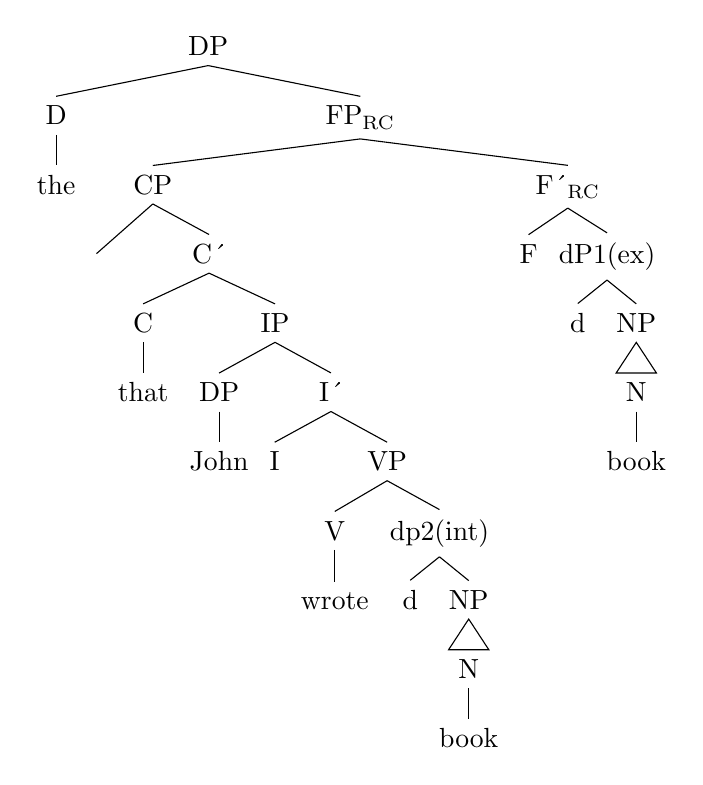
\begin{tikzpicture}[baseline=-0pt, remember picture]
\tikzset{level distance=25pt, sibling distance=1pt}
 \Tree [.DP [.D {the} ] [.FP\textsubscript{RC} [.CP \node (N1) {}; [.C´ [.C {that} ] [.IP [.DP {John} ] [.I´ I [.VP [.V {wrote} ] [.dp2(int) d [.NP \edge[roof]; [. \node (N2) {N}; {book} ] ] ] ] ] ] ] ] [.F´\textsubscript{RC} F [.dP1(ex) d [.NP \edge[roof]; [.N {book} ]]]]]]
 \end{tikzpicture}

Crucial to this idea is that the noun is structurally present twice, once inside and once outside the relative clause,\footnote{In fact, what is structurally present twice, is not only the noun but any projection lower than the indefinite head d.} and deletable in either a raising or a matching fashion. Either, the internal head, dP2, moves to Spec, CP, where it receives operator status and licenses subsequent deletion of the external head (raising), or the external head, dP1, stays in situ and licenses the deletion of the internal head dP2 (matching), cf. \citet[25–45]{cinque:2020:relcl}. This account is argued to be universal and both derivations are accessible in all languages at all times. %\is{raising, matching, dP}

The problem with this account is that evidence for a double-headedness of the noun has only been proven in a small number of languages, including Kombai (Awyu, West Papua; cf. \citealt{vries:2020:greater}) and Wenzhounese (Sinitic; cf. \citealt{hu:2018:new}). In most languages, including English and Japanese (although see \citealt{erlewine:2016:unifying} for possible exceptions), there is only one overt noun, or some version of it. Furthermore, as shown in Chapter \ref{operator}, Japanese shows ample evidence for movement in the form of reconstruction effects, which in turn speaks in favor of either an operator movement or raising derivation. For these reasons, I will not adopt the double-headed structure here, but a simpler structure, and assume operator movement as the operation that derives relative clauses in Japanese.

\subsection{Summary: Indirect modification}

To summarize, indirect modifiers come in two types, full and reduced relative clauses. These modifiers differ in their structural make-up and syntactic height. In this book, relative clauses will be assumed to be derived via movement of an operator from within the relative clause to a Spec, CP, which is co-indexed with the noun and ensures correct interpretability.

\section{Additional accounts}

In this section, I will present ideas from three additional proposal, that differ from the mainline approach in \citet{cinque:2005:deriving, cinque:2017:micro, cinque:2010:adj, cinque:2020:relcl} in different ways and will all enrich the system defended here. They all share the assumption of a large amount and universal character of functional projections within the DP, but add different ingredients to be adopted in the following. I will focus on what is relevant in these approaches for the purpose of this study.

\subsection{Svenonius: Gradability and intersectivity} \label{svenonius}

\citet[249–250]{larson:2021:rethinking}, in a general critique on cartography (and see \citealt{truswell:2004:attributive, truswell:2009:attributive, svenonius:2008:position, kotowski:2016:adj} and \citealt{kim:2019:syntax} for different languages and categories), mentions the ``problem of rigidity“ according to which such a strict structural selection that we see in cartography should always be reflected in linear order (\citealt{kayne:1994:anti, cinque:2010:adj} etc.) and thus deviations should never occur. However, as \citet{svenonius:2008:position} points out, sometimes the ordering restrictions proposed in \citet{scott:2002:stacked} and similar work seem rather ``tailored" \citep[37]{svenonius:2008:position}. For instance, the order of the modifiers of \textsc{dimension} and \textsc{shape} in \ref{longthick} is rather free. On the contrary, he does point out clear cases where ordering restrictions hold, for example between modifiers of \textsc{dimension} and \textsc{color}, illustrated in \ref{tinyred}. %\is{intersectivity, adjective ordering restrictions}

\ex. \label{longthick} \a. a long thick rope (\textsc{dimension} $\succ$ \textsc{shape})
\b. a thick long rope (\textsc{shape} $\succ$ \textsc{dimension}) \null \hfill\citep[37]{svenonius:2008:position}

\ex. \label{tinyred} \a. tiny red hats (\textsc{dimension} $\succ$ \textsc{color})
\b. ??red tiny hats (\textsc{color} $\succ$ \textsc{dimension} \null \hfill\citep[36]{svenonius:2008:position}

Svenonius dismisses ordering restrictions based on fine-grained semantic categories, and instead argues that such ordering restrictions only arise with modifiers with different levels of gradability (as well as intersectivity). For example, modifiers of \textsc{color}, \textsc{origin} and \textsc{material} are clearly non-gradable, while modifiers of \textsc{dimension}, \textsc{quality} and \textsc{shape} are gradable (countable).

\ex. \a. ??very red / Japanese / metal hat (\textsc{color}, \textsc{origin}, \textsc{material})
\b. very big / nice / round hat (\textsc{dimension}, \textsc{quality}, \textsc{shape})

The different types of modifiers can, according to Svenonius, also be differentiated according to their level of intersectivity, and this can be tested via paraphrasing them with a \textit{for-PP}. Only subsective modifiers, for instance of \textsc{dimension}, allow such a paraphrase, intersective modifiers, for example of \textsc{color}, do not (cf. \citealt{mckinney:2011:adj} and \citealt{cinque:2014:semantics}).

\ex. \a. big for a butterfly \null \hfill subsective
\b. *red for a hat \null \hfill intersective

\citet[sec. 4.3]{svenonius:2008:position} proposes that the DP incorporates the functional projections nP, reserved for non-gradable intersective modifiers, and SortP for gradable, subsective modifiers. Since non-gradable intersective modifiers, for instance of \textsc{color}, seem to be closer to the noun than gradable subsective modifiers of \textsc{dimension}, SortP hierarchically precedes nP. This yields the following hierarchy.\footnote{PlP is a projection hosting plural morphemes and UnitP (also ClP; \citealt{svenonius:2022:span}) hosts numerals. This hierarchy mirrors the types and ordering principles of different classifiers found in classifier-languages, an idea taken from \citet{borer:2005:in}, see also \citet{rijkhoff:2002:noun} and \citet{zamparelli:2000:layers}.} %\is{adjective ordering restrictions}

\ex. UnitP $>$ PlP $>$ SortP $>$ nP $>$ NP \null \hfill \citep{svenonius:2008:position}

Svenonius does not make any reference to the difference between direct and indirect modifiers, so what exactly merges in SortP and UnitP is neither limited to lexemes of certain word classes nor of specific modification types. Instead, modifiers merge in ``whatever position makes sense for their interpretation’’ \citep[39]{svenonius:2008:position}. This is undesirable for our aim of deriving a DP structure that incorporates the aspect of modification type. A concrete problem is furthermore that ordering restrictions among categories of the same degree of intersectivity, for example \textsc{color} and \textsc{nationality}, are not predicted, although we do see these even in English as also pointed out in \citet{panayidou:2013:in}.

\ex. ??Chinese blue vase

The same holds true for a recent proposal extended in \citet{manzini:2025:left}, who argues in a similar vein that ordering is not determined directly in the syntax, and never based on fine-grained functional projections, but is the result of externalization \citep{chomsky:2013:problems}. Nevertheless, as she proposes, adjectives merge at different levels of the DP, depending on whether they are gradable. Concretely, \citet[10–16]{manzini:2025:left} proposes that gradable adjectives merge at the edge of the nP phase, assuming that the DP can be divided into several phases, while non-gradable adjectives merge as complements of nP.\footnote{\citet{manzini:2025:left} does not make the same reference to intersectivity, concretely since, as she argues, intersectivity and subsectivity are semantic concepts respectively and, according to her, are difficult to argue to have syntactic dimensions. Furthermore, she provides the data point in \Next where an intersective adjective precedes a subsective adjective in English, contrary to expectation. It should be noted, however, that different mechanisms might be at play here, such as scope dependencies, similar to cases addressed in
Chapter \ref{optionality} for Japanese.

\par

\ex. It is not true that there are no beautiful good linguists. \null \hfill \citep[10]{manzini:2025:left}

\par
}
However, data points such as those provided above are equally problematic for her account.

Besides the idea that fine-grained functional projections might not (always) be at stake, what will also be adopted from Svenonius is a specific projection on the right edge of the DP for idiomatic modifiers. Arguably, such modifiers are embedded in category-less root phrases \citep{marantz:1997:no}. Such root phrases are embedded at the nP level. That they occupy the position right above the noun, becomes evident since nothing can intervene between idiomatic modifiers and the noun they modify without changing the idiomatic meaning \citep[36–38]{svenonius:2008:position}. %\is{idiomatic modifiers}

\ex. \a. Minnesotan wild rice
\b. wild Minnesotan rice (only `uncultivated rice from Minnesota’) \\ \null \hfill\citep[36–37]{svenonius:2008:position}

\subsection{Laenzlinger: Split-DP} \label{laenzdp}

Christopher Laenzlinger (\citeyear{laenzlinger:1998:comparative, laenzlinger:2005:french, laenzlinger:2010:cp, laenzlinger:2011:elements, laenzlinger:2015:the}) focuses on the parametric differences between Romance (French) and Germanic and extends his findings to a cross-linguistic perspective. He presents a study which discusses the CP and DP in 14 typologically diverse languages, one of these languages being Japanese. His approach and DP-structure are essentially similar to Cinque’s modulo certain differences. %\is{split-DP}

What is crucial for the account presented in this study is his adoption of a DP-external domain, a `\textit{Vorfeld}’ or `ω-domain’ as he calls it, above the `middle field’ and `low field’ (\citealt[7]{laenzlinger:2011:elements}; see \citealt{grohmann:2003:prolific} for a similar account). This area can be reached via individual movement of modifiers and is headed by a dedicated D-projections `DP\textsubscript{determination}’ above the \textit{internal} `DP\textsubscript{deixis}’ \citep[668–669]{laenzlinger:2005:french}. The availability of two D-positions accounts for the overt occurrence of multiple D-elements in certain languages (including Lakota and Urama, see \citealt[187–193]{becker:2018:articles}) as well as well-known phenomena such as Romance superlatives \citep{bruge:2002:positions, bernstein:2001:focusing} or Greek determiner spreading (\citealt{androutsopoulou:1995:ds}, but see \citealt{lekakou:2012:poly} for an alternative claim). Furthermore, the necessity of a left periphery in the nominal realm has been put forth by various authors to account for high topic and focus positions and movement to those (\citealt{giusti:1996:is, dimitrova:1998:fragments, ihsane:2001:specific, aboh:2004:topic, aboh:2006:when, grohmann:2003:prolific, grohmann:2015:demonstrative}; cf. \citealt[173–178]{laenzlinger:2011:elements}). In DPs with only one determiner, this determiner always starts in the lower DP but can move up in case material has moved above it \citep[667]{laenzlinger:2005:french}.

The necessity of a left periphery as a landing site for modifiers serves mainly the purpose of accounting for otherwise inexplicable placement of modifiers. As Laenzlinger assumes that the canonical position of adjectives in French is postnominal, which is the result of NP-movement to satisfy agreement between adjective and noun, pied-piping the adjective in the process \citep[657–662]{laenzlinger:2005:french}, prenominal adjectives are only possible in the following circumstances which are all related to deictic or pragmatic contributions \citep[666]{laenzlinger:2005:french}. This echoes the arguments from the other authors mentioned above who proposed a left periphery to account for high modifiers with a topic or focus interpretation. %\is{split-DP, left periphery, focus, topic}

\ex. \a.They have an emphatic or subjective interpretation such as \textit{superbe} `superb’.
\b. They are quantifiers.
\c. They appear in weak forms (\textit{gros} in the literal sense of `big’ as opposed to `grand’).

Such modifiers move to the specifier position of dedicated projections FocP/SubjectiveP, for focused/subjective adjectives, QuantP, for quantifiers, and WeakP for weak forms of French adjectives respectively \citep[666–668]{laenzlinger:2005:french}. In a DP such as \ref{laenzlinger example}, first the NP has moved cyclically to an agreement position in the DP-external domain, where it checks agreement with the adjectives \textit{rouges} `red’, \textit{magnifiques} `beautiful‘ and \textit{petites} `small’. The adjective \textit{petites} subsequently moves to WeakP in the left periphery for pragmatic reasons \citep[667]{laenzlinger:2005:french}. %\is{split-DP, French}

\exg. de petites voitures rouges magnifiques \\
\textsc{det} small car red beautiful\\
`beautiful small red cars’ \null \hfill \citep[668]{laenzlinger:2005:french} \label{laenzlinger example}

The DP-structure, given in hierarchical format, proposed by \citet{laenzlinger:2005:french, laenzlinger:2011:elements} reads as follows.

\ex. DP\textsubscript{external/deictic} $>$ QuantP $>$ FocP $>$ WeakP $>$ FP\textsubscript{AgrNP} $>$ DP\textsubscript{internal/determination} $>$ FP\textsubscript{PP} $>$ FP\textsubscript{AgrNP} $>$ FP\textsubscript{Pred} $>$ FP\textsubscript{Adj} $>$ nP $>$ NP \null \hfill \citep[35]{laenzlinger:2011:elements}

Notably, Laenzlinger does not present a systematic difference between direct and indirect modification and his projection PredP (FP\textsubscript{Pred}) is reserved for what he calls ``external adjectival predicates” \citep[670]{laenzlinger:2005:french} explaining cases of three postnominal adjectives in French. This scenario is atypical, but possible, if the final one receives an emphatic reading such as in \textit{une voiture rouge italienne MAGNIFIQUE} `a BEAUTIFUL red Italian car’ \citep[663–664, 671–672]{laenzlinger:2005:french}.\footnote{Also, the question remains why languages should exist that have agreement, but where prenominal adjectives are inflected, but postnominal adjectives uninflected, a point also raised in \citet[20, Fn. 9]{bortolotto:2016:RA}. A good example is German, where inflected attributive adjectives in prenominal position are the standard case, but postnominal adjectives are possible, in which case they are not inflected (cf. \citealt{trost:2011:whiskey}) as in \textit{Whisky pur} `pure whiskey’ \citep[383]{trost:2006:die}.}

The main point to be adapted from Laenzlinger is the left periphery within the DP and the possibility for individual movement. Specifically, Japanese also freely exhibits different kinds of modifiers in a position above demonstratives, among them quantifiers and direct modifiers, but no pragmatic factors are detectable. %\is{split-DP, adjective ordering restrictions}

\ex. \ag. takusan-no ano hon\\
a.lot-\textsc{no} that book\\
`those many books’
\bg. izen-no kono rūru\\
former-\textsc{no} this rule\\
`this former rule’

\subsection{Kim: A tripartite DP-structure based on Korean} \label{kimsaccount}

\citet{kim:2019:syntax} blends and amends the two preceding analyses of \citet{svenonius:2008:position} and \citet{laenzlinger:2005:french} and enriches them with her own ideas drawing from Korean data. Essential to her account as well is a tripartite DP-structure consisting of three layers: A \textit{High Field} headed by DP\textsubscript{d(eixis)/r(eferential)}, a \textit{Middle Field} headed by DP\textsubscript{q(uantification)} and a \textit{Low Field} headed by DP\textsubscript{p(redication)}. These DPs license [deictic, referential, definite], [quantificational] and [predicative] features respectively \citep[123]{kim:2019:syntax}.\footnote{These DPs correspond to the layered structural mapping of satellites around a nominal or verbal nucleus proposed in \citet[218]{rijkhoff:2002:noun}, and also to three different types of nominals, namely referential, quantificational and predicative \citep[114]{kim:2019:syntax}.} Furthermore, she assumes independent movement of modifiers for reasons of feature-checking (and potentially at LF for semantic/pragmatic reasons) and even of whole DP domains and all material contained in them. Every functional projection, and this includes every DP projection, can multiply and ``create“ additional functional projections of the same kind in an adjunct fashion.\footnote{``FPs of the same kind can be created in the left periphery of a DP structure as needed, forming an adjunction structure" \citep[121]{kim:2019:syntax}, cf. \citet{koopman:2000:verbal}.} %\is{split-DP}

What will be adopted here, besides the split-DP also argued for in \citet{laenzlinger:2005:french, laenzlinger:2011:elements}, is her projection SpplP (SupplementaryP) situated above the highest DP and dedicated to \textit{supplementary} relative clauses, which are not properly \textit{integrated} in the DP \citep[116–119]{kim:2019:syntax}.\footnote{Note that \textit{supplementary} is not equal to \textit{non-restrictive}. While supplementary relative clauses are always non-restrictive, both, non-restrictive and restrictive, relative clauses can be integrated parts of the internal DP \citep[120]{kim:2019:syntax}.} She gives the following example (from \citealt{huddleston:2005:student}). %\is{non-restrictive relative clauses}

\ex. The doctor, [with no name tag on], got into serious trouble. \\ \null \hfill \citep[117]{kim:2019:syntax}

A (reduced) relative clause such as \textit{with no name tag on} is not essential to the DP, but \textit{supplementary}. It is base-generated in the left periphery outside the scope of D. In Japanese, non-restrictive, or supplementary, relative clauses also obligatorily occur above demonstratives (example adapted from \citealt[7–8]{ishizuka:2008:RC}). %\is{non-restrictive relative clause}

\exg. Ito-san-ni-wa musuko-ga hitori i-ru. [[Sakunen isha-ni nat-ta] sono musuko-ga] kekkon-shi-ta.\\
Ito-Mr./Mrs.-\textsc{loc-top} son-\textsc{nom} one be-\textsc{prs} last.year doctor-\textsc{loc} become-\textsc{pst} that son-\textsc{nom} marriage-do-\textsc{pst}\\
`Mr./Mrs. Ito has one son. This son, who happened to become a doctor last year, got married.' \\ \null \hfill non-restrictive relative clause $\succ$ demonstrative $\succ$ N

In the lower DP domain, Kim assumes the same projections as \citet{svenonius:2008:position} and adds a projection for possessive modifiers and demonstratives called LocP (the satellite `\textit{Location}’ in \citet{rijkhoff:2002:noun}). She offers the following hierarchy. %\is{split-DP}

\ex. {RC\textsubscript{Sppl}} $>$ DP\textsubscript{deictic/referential} $>$ DP\textsubscript{quantification} $>$ DP\textsubscript{predication} $>$ FocP $>$ LocP $>$ UnitP $>$ PlP $>$ SortP $>$ nP $>$ $\sqrt{}$P $>$ NP \null \hfill \citep[132]{kim:2019:syntax}

Another important assumption to be adopted (see Chapter \ref{size,indirect}) is the unification of full and reduced relative clauses to one type of relative clause of the same size.

\section{Further issues}

In this section, I raise two additional issues. One anticipates potential problems that come with cartography, in the other, I briefly mention previous approaches to Japanese as part of this research program.

\subsection{Potential problems of cartography} \label{problemscarto} %should i divide this chapter?

A system as rigid as cartography cannot be free of problems and criticism. Anticipating the discussion, I will discuss several potential problems below.\footnote{For this section, consider the recent discussions in \citet{manzini:2025:left} and \citet{cinque:2025:superiority}.}

One objection concerns the existence of movement operations for the sake of order and devoid of syntactic and semantic constraints, often dubbed ``meaningless movement’’. Several researchers have argued that this kind of movement should be kept apart from narrow syntax (most notably see \citealt{chomsky:2019:generative} and references cited therein). Recall from Chapter \ref{japanese no movement} that no NP-movement needs to be assumed in Japanese since the noun is always the final element in the DP.\footnote{For meaningless movements also see \citet{hall:2015:spelling}.} %\is{meaningless movement}

While this is a more ideological point, a more concrete point that begs further discussion in the future is the nature of the cross-linguistic restrictions on movement operations. How are they spread across different languages and language groups? Why do we only witness a particular type of movement, for instance progressive pied-piping, in a given language, while other languages allow both types (see footnote \ref{footnotemovement} in Chapter \ref{left-right})? Furthermore, experimental approaches have cast doubt on universal syntactic principles and related ordering principles rather to cognitive factors, such as subjectivity and information gain. See \citet{scontras:2017:sub, dyer:2024:evaluating}, the works cited therein and similar works by the same authors.

Sometimes, even specific subclasses of modifiers in a given language are restricted to specific positions and suggest a restriction to one particular type of movement. An interesting case are uninflectable adjectives of the type \textit{blu} `blue’ in Italian, and perhaps in other Romance languages. Italian color adjectives, although restricted, can appear in prenominal and postnominal position, but this is never possible for uninflectable color adjectives such as \textit{blu} illustrated below, same as for Relational Adjectives in this and other Romance languages. %\is{relational modifiers, Italian}

\ex. \ag. la (rossa) distesa (rossa) del mare (Italian)\\
the red.\textsc{f.sg} expanse.\textsc{f.sg} red.\textsc{f.sg} of.the sea\\
`the red expanse of the sea'
\bg. la (*blu) distesa (blu) del mare\\
the blue.\textsc{$\emptyset$} expanse.\textsc{f.sg} blue.\textsc{$\emptyset$} of.the sea\\
`the blue expanse of the sea' \null \hfill \citep[110]{mattiuzzi:2023:influential}

Such adjectives pose a problem for standard cartographic accounts, since no obvious relation between morphology and syntax can be drawn. Specifically, there is no obvious reasons why this specific type of modifiers must be subject to pied-piping. The problem also extends to the system of \citet{laenzlinger:2005:french, laenzlinger:2011:elements}, which would predict only agreeing adjectives to surface postnominally. For recent discussion see also \citet{mattiuzzi:2023:influential}.

Equally problematic are data points, provided by several authors from different languages, that show that direct modifiers (adjectives) adhere to the strict ordering principles dictated by cartography cross-linguistically to different degrees (see for an overview \citealt{manzini:2025:left}). I refer the reader to Chapter \ref{discussiondirect}, where I discuss this point, specifically with regard to Japanese, but also to Persian and Modern Greek. Here, I would like to exemplify this point with recent data from Naasioi, a Papuan language. See Chapter \ref{more languages} for discussion on this and another problematic language.

\citet{brown:2024:adj} provides very clear evidence that adjectives in Naasioi which are unequivocally direct do not have to adhere to ordering principles, as shown below (see the relevant paper for evidence that the provided adjectives are direct).

\ex. \ag. pangkaing mutaanu mosi (Naasioi)\\
big black dog\\
\bg. mutaanu pangkaing mosi\\
black big dog\\
`big black dog’ \null \hfill \citep[428]{brown:2024:adj}

As I will argue in this book, such cases are unproblematic if we assume that the nature of the functional projections available in the direct domain of the DP are subject to cross-linguistic variation.

Finally, a potential problem concerns the presumably infinitive amount of functional heads present in the nominal, and also the clausal, domain. Recall that, if we take the cartographic idea seriously, every new category found in a certain language must be present in the functional spine of all languages. This point is also raised in \citet{larson:2021:rethinking}, who also reports the first of the two quotes below.

\ex. \a. The cartographic approach follows this idea in assuming that all languages share the same principles of phrases and clause composition and the same functional make-up of the clause and its phrases. \citep[68]{cinriz:2010:carto}
\b. Comparison of many different languages may provide evidence for determining the precise relative order of the different projections by combining the partial orders overtly manifested by different languages into what, in principle, should be a unique consistent order/hierarchy, imposed by UG. \citep[72]{cinriz:2010:carto}

A concrete problem arises if a modifier occurs that cannot readily be assigned to any of the existing categories of functional projections. An obvious solution would be to establish a new functional projection. But this would, at some point, potentially lead to an overabundance of categories, which is called the `\textit{Problem of Plenitude}’ in \citet[248–249]{larson:2021:rethinking}. This problem is circumvented in this study by assuming unspecific projections, an assumption that also solves the `\textit{Problem of Rigidity}’ (\citealt[249–250]{larson:2021:rethinking}) which concerns the lack of expected ordering principles between two modifiers of different categories. %\is{problem of plenitude, problem of rigidity}

In sum, cartography faces the problems of meaningless movement, ordering derviations, plenitude and rigidity. As its counter-advocates argue, it overgenerates and undergenerates at the same time \citep{larson:2021:rethinking, manzini:2025:left}. Still, this research topic is extremely powerful and offers the right tools and principles for an in-depth investigation of the Japanese DP. Especially important is the assumption of two different sources of modifiers and their different characteristics and derivations, furthermore theoretically predicting linear precedence. Since even though there might be more lenient cases, some ordering principles still do exist. All these issues will be further addressed in Chapter \ref{discussiondirect}.

\subsection{Japanese and cartography: Previous analyses and relevance}

\subsubsection{Laenzlinger on Japanese DP} \label{Laenz}

\citet{laenzlinger:2010:cp, laenzlinger:2011:elements} draws many implications for his universal DP structure from Japanese as a strict head-final language. His typological study is to my knowledge the only one that looks at the Japanese nominal domain in line with cartography. However, other than his detailed analysis of the Japanese clause, his discussion of the Japanese noun phrase falls out short. He gives the following example of three modifiers adhering to the expected order \textsc{quality} $\succ$ \textsc{dimension} $\succ$ \textsc{color}.

\exg. \label{chiisa}subarashi-i chiisa-na aka-i kuruma \\
wonderful-\textsc{i} small-\textsc{na} red-\textsc{i} car\\
`wonderful small red car(s)’ \hfill \citep[189]{laenzlinger:2011:elements}

He claims that the expected order is also the preferred one, but that modifiers in general can be permuted without a change in meaning or ``special focus effect(s)” \citep[190]{laenzlinger:2011:elements}. He concludes that ``at first sight Japanese (and also Tatar) pose a problem for previous theories to nominal modification and modifier ordering’’ (ibid.) and, as many researchers have done before him, solves this problem by analyzing alls adjectives as stacked relative clauses predicting possible permutation. This finds support in his analysis of \textsc{i} (and \textsc{na}) as tense morphemes (\citealt[191]{laenzlinger:2011:elements}, Fn. 106). %\is{adjective ordering restrictions, rentaishi}

It was already shown that direct modification does exist in Japanese, so this analysis cannot be correct. It remains furthermore unclear why there should be a preferred order of modifiers in the first place, if permutation is always allowed, and why this order should be as in English. Another major problem is that his example \ref{chiisa} contains the attributive-only lexeme (\textit{rentaishi}) \textit{chiisa-na} `small’, which cannot function as a predicate, hence cannot be predicative and be embedded in a relative clause as shown in \ref{rentaishilaenz}. This group of modifiers is the topic of Chapter \Ref{rentaishi}.

\ex. \label{rentaishilaenz} \ag. chiisa-na ie\\
small-na house\\
`small house'
\bg. *Kono ie-wa chiisa-da.\\
this house-\textsc{top} small-\textsc{cop}\\
(`This House is small.’)

\subsubsection{Other Analyses}

Several studies discuss the Japanese clause from a cartographic perspective: \citet{endo:2007:locality} looks at the left periphery in Japanese, integrating Japanese into Rizzi's account on locality and Relativized Minimality (\citeyear{rizzi:1997:the}). Other authors have looked at the right periphery (cf. overview in \citealt{saito:2015:carto}). \citet{ueda:2008:person} develops a hierarchy of modals expressed through sentence-final particles, \citet{saito:2013:sentence} discusses various sentence types and movement to the right periphery, and \citet{saito:2012:deriving} develop a hierarchy of complementizers and sentence-final particles which is refined in \citet{saito:2015:carto}. What is interesting about all these studies is that they do find a hierarchy and derive generalizations that are empirically and theoretically valid, but for the clause, again highlighting the more controversial and recalcitrant nature of the DP.

\subsubsection{Narrog (2009)} \label{narrog}

\citet{narrog:2009:mod} is a very detailed study on the ordering of modal elements in Japanese and, to my knowledge, the only one that combines classical approaches from Japanese linguistics and cartography. The author identifies twelve affixes, 20 periphrastic constructions, six verbal inflections and an infinite number of modal adverbs in Japanese \citep[71–76]{narrog:2009:mod} and establishes ordering and scope principles based on a corpus study. He compares his findings to those of Cinque’s adverbial hierarchy (\citeyear{cinque:1999:adverbs}) and eventually rejects the cartographic model. Besides several mismatches,\footnote{For example, Cinque only has one position for evidentiality, Narrog observes three which all occupy different positions in relation to modal and epistemic markers.} the biggest problem, Narrog claims, is the interaction of modal categories with those of tense and aspect in his model which differs greatly form Cinque’s version \citep[233–234]{narrog:2009:mod}. In the end, Cinque’s model is deemed too abstract and ``fictional” for Narrog. He claims such models can only be maintained if they are ``understood as idealizations, or rough approximations to actual language data” \citep[243]{narrog:2009:mod}. Furthermore, he calls into question the ``psychological reality of the existence of the same universal hierarchy of categories in every sentence of any language of the world” (ibid.), again pointing towards the problem of rigidity \citep{larson:2021:rethinking}. Even though he ends up rejecting cartography as an explanation for the problems he is concerned with, his study is still relevant as it produces a very substantial hierarchy on the basis of empirical data that could in turn be checked for other languages. This hierarchy is picked up in the discussion on adverbials in Chapter \ref{cinque adj}. %\is{modality}

\subsubsection{Takamine (2010)} \label{takamine}

\citet{takamine:2010:hierarchy} looks at the order of prepositional phrases in Japanese following the theoretical framework of \citet{cinque:1999:adverbs, cinque:2006:complement} and \citet{schweikert:2005:order}. Because Japanese is a scrambling language with a variety of possible orders, it is necessary to test the order of PPs in a neutral environment. She looks at nine different categories and employs three tests for their interaction. She arrives at the following general hierarchy (see for discussion and references \citealt[58-83]{takamine:2010:hierarchy}).

\ex. \emph {Hierarchy of PPs in Japanese (\citealt[94]{takamine:2010:hierarchy})}\\
\textsc{temporal} $>$ \textsc{locative} $>$ \textsc{comitative} $>$ \textsc{reason} $>$ \textsc{source} $>$ \textsc{goal} $>$ \textsc{instrumental}/\textsc{mean} $>$ \textsc{material} $>$ \textsc{manner}

Takamine’s study is relevant for two reasons. First, because she shows that word order in Japanese is not as random as it appears at first sight. Second, this hierarchy bears some resemblance to the nominal domain. This is acknowledged in \citet{bortolotto:2016:RA}, who compares Takamine's and Rae's hierarchies (\citeyear{rae:2010:ordering}) to her hierarchy of relational adjectives in Romance presented above. %\is{prepositions}

\section{Chapter Summary}

This chapter introduced the theoretical background of this study focusing on the core ideas of the cartographic account and the difference between direct and indirect modifiers. It also picked up all relevant ideas to be implemented in the account of the Japanese DP to follow. The chapter ended with a quick, condensed overview over problematic aspects of cartography and the few studies which pursued an analysis of certain aspects of Japanese syntax under a cartographic lens, highlighting the perhaps surprising lack of studies concerned with the nominal domain.

\chapter{The Japanese DP} \label{theoreticalassumptions}

In this chapter, I present in detail the two theoretical contributions of this book. I start out with the structure of the DP. This structure, which I assume to be universal, is in line with the assumptions in cartography outlined in the preceding chapter, but enriched with the Japanese data. It is not only better suited for handling this data, but also makes important predictions for the structure of the DP, abandoning the strict connection between direct modification and rigid modifier order. I start with an overview over the complex split-DP structure and the three relevant areas. I then briefly go over each relevant area in a bottom-up fashion. Since both, the direct and indirect domain, the main topics of this study, will each receive detailed explanations in the following two chapters, the discussion on these areas will be kept comparatively short here, but I spend some more time on the DP-external domain, i.e. the left periphery.

The second part of this chapter is dedicated to the internal structure of modifiers, with a special focus on the monomoraic elements co-occurring with non-verbal modifiers, especially \textsc{no}. I will put forth an account of these elements as syntactic heads in the spirit of \citet{rubin:1993:category, rubin:1994:mod, rubin:1996:transparent}, which license modifiers in attributive position. I thereby introduce an additional functional head in the internal structure of modifiers, informing our knowledge of the DP as a whole. I argue that all kinds of modifiers are licensed by this head, irrespective of word class and modification status, but discuss some difficult cases of CPs with overt tense heads where \textsc{mod} is covert.

\section{The structure of the Japanese DP} \label{japanesedp}

I adopt the basic cartographic assumptions of a universal spine within the clause and the DP, in which the hierarchically final element is the lexical head, i.e. N or V. This head can be subject to phrasal movement, but only to the left, never to the right \citep{kayne:1994:anti, cinque:2005:deriving, cinque:2023:linearization}, although, as shown in Chapter \Ref{sectioncarto}, in Japanese, and potentially other strictly head-final languages, movement of the lexical head does not occur. Rather, certain modifiers can move to a higher position, especially the DP-external domain, individually, as also argued elsewhere (cf. \citealt{kim:2019:syntax, laenzlinger:2005:french, laenzlinger:2011:elements}). The extended projection of both lexical heads contains a (potentially) infinite amount of functional projections, that serve as merging and landing sites for various types of modifiers.

Furthermore, I assume the DP to be split, paralleling accounts on the split-CP \citep{rizzi:1997:the, grohmann:2003:prolific, laenzlinger:2011:elements,}, into two large domains: The DP-external domain, essentially the left periphery of the DP, and the DP-internal domain \citep{kiss:1998:identificational, kiss:2007:topic, giusti:1996:is, dimitrova:1998:fragments, ihsane:2001:specific, aboh:2004:topic, aboh:2006:when, laenzlinger:2005:french, kim:2019:syntax}. The DP-internal domain is made up of two subdomains: The indirect and the direct domain.\footnote{Note that the tripartite divide I assume to hold for the DP does not coincide with the tripartite structure of other authors \citep{laenzlinger:2011:elements, grohmann:2003:prolific} who assume a divide into an agreement and a theta domain for the lower part.}

The complete structure of the Japanese DP is given in the figure below with the left part of the tree representing the DP-external domain and the right part the DP-internal domain, which starts where the DP-external domain ends. The thresholds between the three domains are marked in boldface. Recall that I indicate the indefinite head d as the threshold between the direct and the indirect domain following \citet{cinque:2010:adj, cinque:2020:relcl}, but that this head does not play a major syntactic role in my system since I do not assume the double-headed structure for relative clauses (see Chapter \ref{dP}).

\newpage

\begin{figure}
 \centering
 \begin{subfigure}{0.5\textwidth}
 \centering
 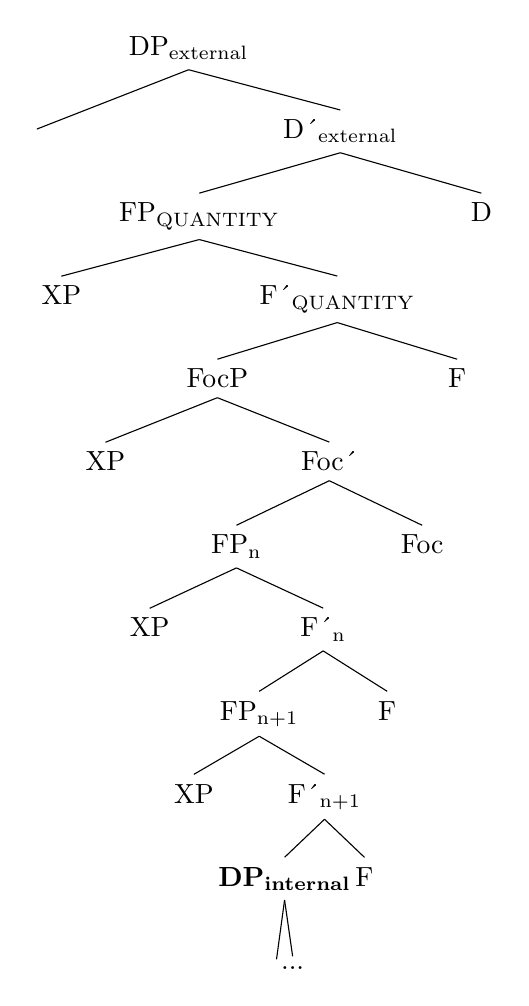
\begin{tikzpicture}[baseline=0pt, remember picture]
\tikzset{level distance=30pt, sibling distance=-5pt}
 \Tree [.DP\textsubscript{external} {} [.D´\textsubscript{external} [.FP\textsubscript{QUANTITY} XP [.F´\textsubscript{QUANTITY} [.FocP XP [.Foc´ [.FP\textsubscript{n} XP [.F´\textsubscript{n} [.FP\textsubscript{n+1} XP [.F´\textsubscript{n+1} [.\textbf{DP\textsubscript{internal}} {} ... ] F ] ] F ] ] Foc ] ] F ] ] D ]]
\end{tikzpicture}
 \end{subfigure}%
 \begin{subfigure}{0.5\textwidth}
 \centering
 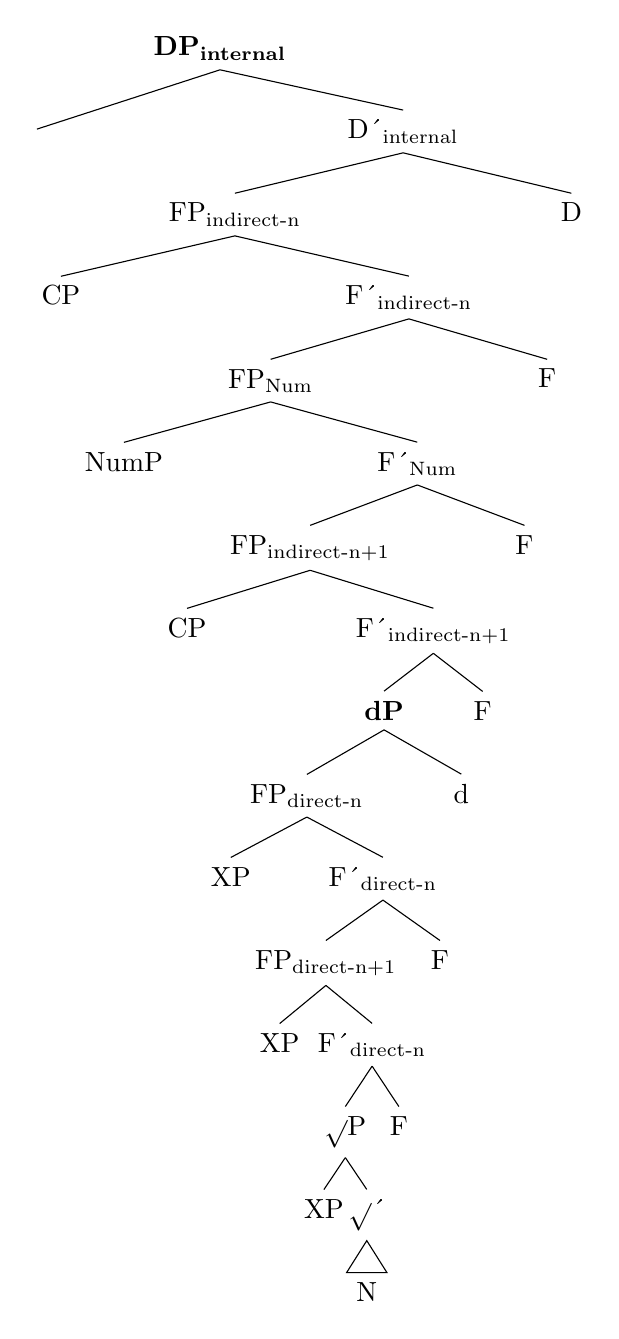
\begin{tikzpicture}[baseline=0pt, remember picture]
\tikzset{level distance=30pt, sibling distance=-5pt}
 \Tree [.\textbf{DP\textsubscript{internal}} {} [.D´\textsubscript{internal} [.FP\textsubscript{indirect-n} CP [.F´\textsubscript{indirect-n} [.FP\textsubscript{Num} NumP [.F´\textsubscript{Num} [.FP\textsubscript{indirect-n+1} CP [.F´\textsubscript{indirect-n+1} [.\textbf{dP} [.FP\textsubscript{direct-n} XP [.F´\textsubscript{direct-n} [.FP\textsubscript{direct-n+1} XP [.F´\textsubscript{direct-n} [.$\sqrt{}$P XP [.$\sqrt{}$´ \edge[roof]; {N} ] ] F ] ] F ] ] d ] F ] ] F ] ] F ] ] D ] ]
\end{tikzpicture}
 \end{subfigure}
 \caption{Structure of the Japanese DP}
 \label{fig:Structure of the Japanese DP2}
\end{figure}


I make the following specific assumptions and predictions for the functional inventory of the three relevant areas.

\ex. \a. \textit{The DP-external domain}, i.e. the left periphery, includes functional projections that host the following elements: A projection for quantifiers, which most probably move there from the direct domain, projections for non-restrictive relative clauses, which merge in the left periphery outside the scope of D, and a projection for focused modifiers, which can optionally move there but are not required to. Furthermore, the left periphery contains an unspecified amount of available functional projections for direct as well as restrictive indirect modifiers which optionally move there out of their respective domains. Those unspecific projections are labeled FP\textsubscript{n}, FP\textsubscript{n+1}, in order to highlight structural hierarchy.
\b. \textit{The indirect domain} is situated higher than the direct domain within the DP-internal domain. It contains (a potentially infinite amount of) functional projections dedicated to indirect modifiers, but those are not differentiated based on different types of indirect modifiers, i. e. full and reduced relative clauses. The indirect domain furthermore encompasses a dedicated projection for numerals and functional projections reserved for indirect modifiers precede and follow this projection.
\c. \textit{The direct domain} is situated below the indirect domain within the DP-internal domain. It contains (a potentially infinite amount of) functional projections hosting direct modifiers. Those projections are not dedicated to modifiers of specific semantic categories. Instead, they are unspecific. Again, structural hierarchy is indicated via the labels FP\textsubscript{n}, FP\textsubscript{n+1}, etc., but this hierarchy only becomes relevant in cases where scope restrictions play a role. The only dedicated functional projection within the direct domain is reserved for idiomatic modifiers and directly c-commands the noun.

\newpage

\subsection{Internal DP: Direct domain} \label{internaldirect}

The direct domain is situated below the indirect domain within the DP-internal domain, making it the lowest area inside the DP, directly above the noun. In the figure below, only the internal DP is displayed and the direct domain is circled.

%\newpage

\begin{figure}[H]
\centering

 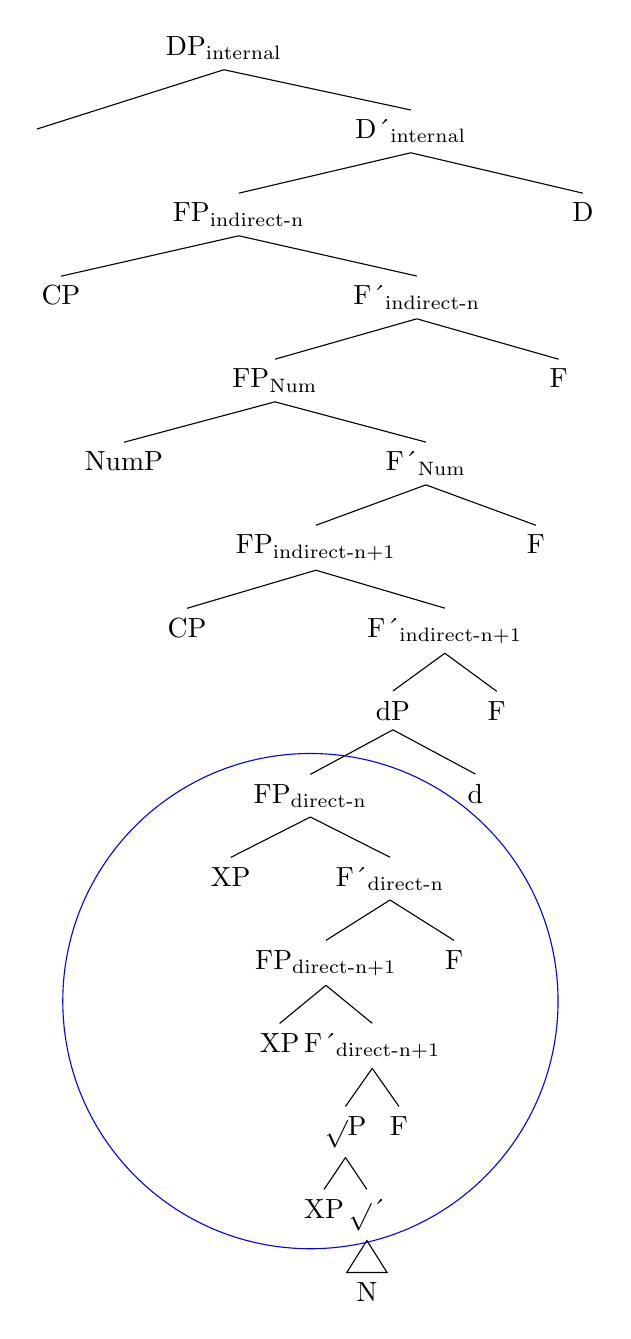
\begin{tikzpicture}[baseline=0pt, remember picture]
\tikzset{level distance=30pt, sibling distance=-5pt}
 \Tree [.DP\textsubscript{internal} {} [.D´\textsubscript{internal} [. \node (indirect1) {FP\textsubscript{indirect-n}}; CP [.\node (indirect0) {F´\textsubscript{indirect-n}}; [.FP\textsubscript{Num} NumP [.F´\textsubscript{Num} [.FP\textsubscript{indirect-n+1} \node (indirect3) {CP}; [. \node (indirect2) {F´\textsubscript{indirect-n+1}}; [.dP [. \node (direct2) {FP\textsubscript{direct-n}}; XP [. \node (direct0) {F´\textsubscript{direct-n}}; [.FP\textsubscript{direct-n+1} XP [.F´\textsubscript{direct-n+1} [.$\sqrt{}$P \node (direct1) {XP}; [.$\sqrt{}$´ \edge[roof]; N ] ] F ] ] F ] ] d ] F ] ] F ] ] F ] ] D ] ]
 \node[draw,circle,fit= (direct1) (direct2) ] [color=blue] {};
\end{tikzpicture}

 \caption{Structure of the Direct Domain in Japanese}
 \label{fig:Structure of the Direct Domain in Japanese1}
\end{figure}

\newpage


In order to motivate a domain for direct modifiers, it needs to be proven that direct modification does exist in Japanese. Ad already mentioned in the preceding chapters, Japanese does posses the equivalents of non-predicative, that is direct-only, non-intersective \ref{intersectivechap3} and relational modifiers \ref{intersectivechap3} \citep{yamakido:2005:nature, ayano:2010:revisiting, nagano:2016:are, watanabe:2017:attributive}.\footnote{Again, I abstract away from possible predicative use of these modifiers in contrastive and elliptical constructions or contexts in which the copula is a placeholder. See Chapter \Ref{test predication}.} %\is{direct modification}

\ex. \label{intersectivechap3} \ag. Tarō-ga shōrai-no purosakkāsenshu-da.\\
Taro-\textsc{nom} future-\textsc{no} pro.soccer.player-\textsc{cop}\\
`Taro is a future professional soccer player.’
\bg. *Ano purosakkāsenshu-ga shōrai-da.\\
that pro.soccer.player-\textsc{nom} future-\textsc{cop}\\
(`That professional soccer player is future.’)

\ex. \label{relationalchap3} \ag. Denmāku-no / chīku-no isu\\
Denmark-\textsc{no} / teak-\textsc{no} chair\\
`Danish / teak chair'
\bg. *Ano isu-wa Denmāku-da / chīku-da.\\
that chair-\textsc{top} Danish-\textsc{cop} / teak-\textsc{cop}\\
(`That chair is Danish / teak.’)

Next, building on the observation of other authors, for instance \citet{cinque:2010:adj} on Germanic (English) and Romance (Italian), the indirect domain is situated above the direct domain in Japanese as well. \ref{directrcchap3} exemplifies this, showing that the (non-intersective) direct-only modifier \textit{shōrai-no} `future’ must be closer to the head noun than the fairly complex relative clause. The other order is significantly degraded. %\is{relative clauses}

\ex. \label{directrcchap3} \ag. Kare-wa [ōku-no kurabu-ga chūmoku-shi-te-i-ru\textsubscript{RC} [\textbf{shōrai-no} purosakkāsenshu]]-desu.\\
he-\textsc{top} numerous-\textsc{no} club-\textsc{nom} pay.attention-do-\textsc{ger}-be-\textsc{prs} future-\textsc{no} pro.soccer.player-\textsc{cop.pol}\\
`He is a future professional soccer player whom many clubs pay attention to.’
\bg. *Kare-wa [\textbf{shōrai-no} [ōku-no kurabu-ga chūmoku-shi-te-i-ru\textsubscript{RC} purosakkāsenshu]]-desu.\\
\textsc{top} future-\textsc{no} numerous-\textsc{no} club-\textsc{nom} pay.attention-do-\textsc{ger}-be-\textsc{prs} pro.soccer.player-\textsc{cop.pol}\\

As a crucial point of derivation from most cartographic accounts, the direct domain introduced here does not encompass functional projections dedicated to modifiers of specific semantic categories. Instead, it encompasses a possibly infinite amount of unspecific functional projections. This accounts neatly for cases of free ordering among (also in English) ambiguous qualitative modifiers, for instance of \textsc{dimension} or \textsc{color} given in \ref{dimensioncolor}. Crucially, it offers an explanation for the lack of ordering restrictions between direct-only modifiers, for example, the two relational modifiers \textit{Denmāku-no} `Denmark, Danish’ and \textit{chīku-no} `teak’ given in \ref{nationality}. %\is{free ordering}

%\newpage

\ex. \textsc{dimension} vs \textsc{color} \label{dimensioncolor}
\ag. ōki-i aka-i hon\\
big-\textsc{i} red-\textsc{i} book\\
`big red book’
\bg. aka-i ōki-i hon\\
red-\textsc{i} big-\textsc{i} book\\
`red big book’

\ex. \textsc{nationality} vs. \textsc{material} \label{nationality}
\ag. Denmāku-no chīku-no isu\\
Denmark-\textsc{no} teak-\textsc{no} chair\\
`Danish teak chair' \label{denmakuneu}
\bg. chīku-no Denmāku-no isu\\
teak-\textsc{no} Denmark-\textsc{no} chair\\
`teak Danish chair'

As I will show at length in the next chapter, Japanese modifiers also fail to exhibit ordering restrictios based on different levels of gradability and intersectivity, contrary to what is claimed in \citet{svenonius:2008:position, manzini:2025:left}, and neither syntax-external factors such as phonological/prosodic length and word class do seem to play a role. This was already shown in \ref{dimensioncolor}, but is illustrated more clearly in the pair in \ref{quality}: The non-gradable, intersective modifier of \textsc{nationality} \textit{Chūgoku-no} `China, Chinese' and the gradable subsective \textit{na}-adjective of \textsc{quality} \textit{kirei-na} `beautiful’ are fine in either order. Importantly, \textit{kirei-na} is not a direct-only modifier, but actually ambiguous and, thus, could be situated in the indirect domain. However, then it would still be expected to be merged higher, and, in neither case, to occur to the right of the direct-only \textsc{nationality} modifier. %\is{relational modifiers}

\ex. \textsc{quality} vs. \textsc{nationality} \label{quality}
\ag. kirei-na Chūgoku-no kabin\\
beautiful-\textsc{na} China-\textsc{no} vase\\
`beautiful Chinese vase'
\bg. Chūgoku-no kirei-na kabin\\
China-\textsc{no} beautiful-\textsc{na} vase\\
`Chinese beautiful vase'

A significant consequence of the theory, and one point I hope to make clear in this book, is that ordering restrictions lose their status as a prerequisite for direct modification and the two issues, type of modification, direct or indirect, and ordering, become two orthogonal issues.

Crucially, Japanese differs from languages such as English which do exhibit ordering restrictions based on semantic categories within the direct domain. I argue that the reason for this lies in parametric variation, to be discussed in Chapter \ref{units of language}. Specifically, the DP-spine is universal, but there is language-specific variation as to whether functional projections based on fine-grained semantic categories are activated or not \citep{ramchand:2014:deriving, wiltschko:2014:universal}. In other words, some languages possess language-specific entities to form functional projections of \textsc{dimension}, \textsc{color} and so on, but others do not. These language-specific entities correspond to the concept of \textit{Units of Language} given in \citet[1]{wiltschko:2014:universal}. %\is{units of language}

To recapitulate, ordering across two different domains is (rather) strict across languages, including Japanese, which gives evidence for a universal DP-structure incorporating a direct and a higher indirect domain (see also \citealt{ramchand:2014:deriving} and \citealt{wurmbrand:2023:ich} for this idea, mostly with regard to the clause). However, this is not the case within one domain and this is the source of cross-linguistic differences.

In Japanese, the two possible variants of linear order between two modifiers is simply a result of merge order. The modifier merged subsequent to the noun is closer to it in linear order. On the other hand, the canonical word order of two (or more) adjectives of different semantic categories in English (and similar languages) are pre-determined in the syntax, given they are both direct.

A reviewer raises the issue on how we can determine whether a modifier is direct or indirect to begin with. The simple answer is: In most cases, we cannot. However, this is not a problem specific to the account proposed here. As illustrated in Chapter \ref{cartography Cinque}, and specifically Chapter \ref{ambiguities}, most modifiers (adjectives) in English are ambiguous as well and it is precisely their behavior in DPs with more than one modifier that can give an indication of their modification status. But this option is not operationalizable in Japanese. We can only prove that a modifier is direct in Japanese by looking at its behavior in predicative structures, alongside the other characteristics explained thoroughly in Chapter \ref{testsdirect}. On the contrary, clear cases of indirect modifiers in Japanese exhibit complex morphosyntactic structures, i. e. inflection for past or co-occurrence with the canonical copula.

Nominal modifiers in Japanese are therefore licensed by functional projections within the extended noun phrase, which this language shares with other languages. However, it is only direct-only modifiers that are exclusively licensed within the direct domain. And only clearly indirect modifiers are licensed within the indirect domain. For all other modifiers, there is no \textit{a priori} indication as to their modification status and they could be licensed by both types of functional heads. The system here is thus more versatile, compared to standard cartographic accounts. But this versatility is necessary in order to incorporate direct(-only) modifiers in the system, while still acknowledging their lack of ordering restrictions among each other.

Before closing this subsection, I will point out two cases of strict ordering observable in the direct domain in Japanese. The first concerns cases that arise when scope and other external factors play a role (see also \citealt{ramchand:2014:deriving} for the clause). This becomes obvious in the following minimal pair of direct-only modifiers. In a context where the speaker is identifying a vase out of a specific pool (for example at a museum), namely the single German one, \textit{yui'itsu-no} `only’ must take scope over both, the following modifier and the noun, thus over the chunk \textit{Doitsu-no kabin} `German vase’, and not just over \textit{kabin} `vase’. In the same context, the reverse order is odd, and can only mean something akin to `the only vase in Germany' or `the only vase produced in Germany' where the part \textit{German} or \textit{in Germany} constitutes an additional piece of information (Ken Hiraiwa p.c.).\footnote{A factor involved here might be the nominal status of \textit{Doitsu} `German(-y)’. There are similar cases reported in \citet{shimamura:2014:go}.

\par

\ex. \ag. tsumeta-i me-no kusuri\\
cool-\textsc{i} eye-\textsc{no} medicine\\
`cool eye medicine’
\bg. *me-no tsumeta-i kusuri\\
eye-\textsc{no} cool-\textsc{i} medicine \null \hfill \citep[163]{shimamura:2014:go}\\

\par

The noun \textit{me} `eye’ modifies the noun \textit{kusuri} first before the adjective takes scope over the whole chunk. The other order is very hard to interpret.}

%\newpage

\ex. \label{yuiitsuchap3} \ag. [yui'itsu-no [Doitsu-no kabin]]\\
only-\textsc{no} German-\textsc{no} vase\\
`only German vase'
\bg. ??Doitsu-no yui'itsu-no kabin\\
German-\textsc{no} only-\textsc{no} vase\\

In cases such as \ref{yuiitsuchap3}, the modifiers occupy distinct positions and merge must have occurred in a specific order. See Chapter \ref{discussiondirect} for discussion.\footnote{This is also a good argument against scrambling as an alternative hypothesis. If scrambling was always an option, it is questionable why it is not possible when scope is involved. I am grateful to Johannes Mursell for discussion.}

The only type of modifiers with a fixed position inside the direct domain are \textit{idiomatic} modifiers, or more precisely modifiers appearing in \textit{non-free phrases} (see \citealt{kohlich:2024:nonfree}). Such modifiers must appear linearly adjacent to the noun. As illustrated below, the direct-only modifier \textit{kōki-no} `curious' and the following noun form the idiomatic expression \textit{kōki-no manazashi} (alternatively \textit{kōki-no me/shisen}) `curious gaze' and no other modifier can intervene.\footnote{This is not due to the behavior of \textit{minna-no} `everyone's` as presented in the relevant discussion in Chapter \ref{idiomatic}.} %\is{idiomatic modifiers}

%\newpage

\ex. \ag. minna-no kōki-no manazashi\\
everyone-\textsc{no} curious-\textsc{no} gaze\\
`everyone's curious gaze'
\bg. *kōki-no minna-no manazashi\\
curious-\textsc{no} everyone-\textsc{no} gaze\\

Following \citet{svenonius:2008:position}, I assume that idiomatic modifiers are embedded beyond the nP level, in a category-less root phrase $\sqrt{}$P (see \citealt{marantz:1997:no}), which immediately c-commands the noun, yielding the following structure.\footnote{Note that I do not indicate the nP-level when giving complete structures of the Japanese DP.}

\ex. \ag. kōki-no manazashi\\
curious-\textsc{no} gaze\\
`curious gaze'
\b. 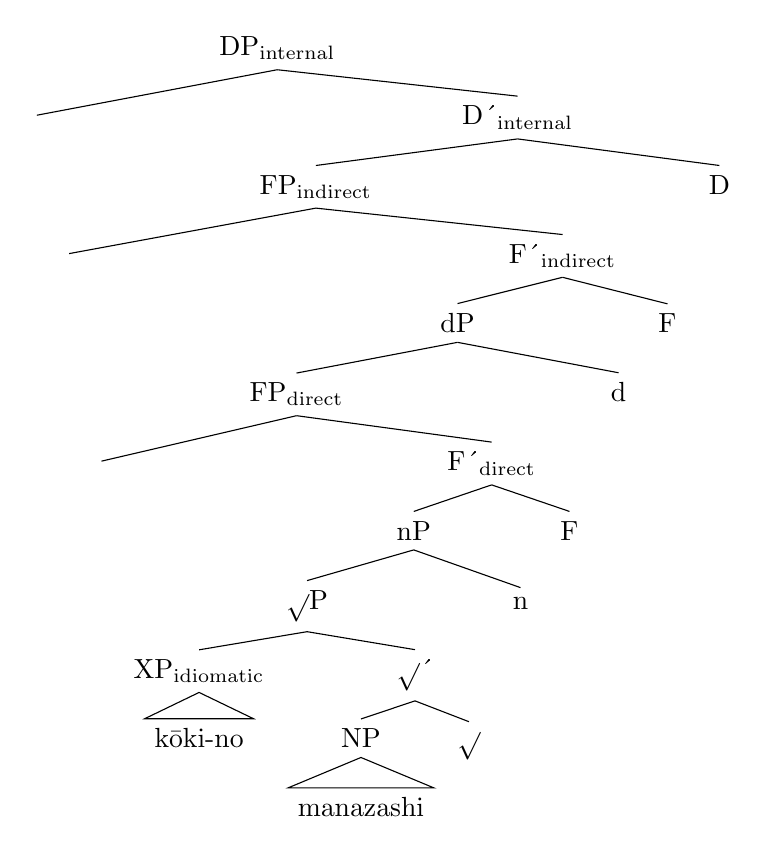
\begin{tikzpicture}[baseline=0pt, remember picture]
\tikzset{level distance=25pt, sibling distance=5pt}
\Tree [.DP\textsubscript{internal} {} [.D´\textsubscript{internal} [.FP\textsubscript{indirect} {} [.F´\textsubscript{indirect} [.dP [.FP\textsubscript{direct} {} [.F´\textsubscript{direct} [.nP [.$\sqrt{}$P [.XP\textsubscript{idiomatic} \edge[roof]; kōki-no ] [.$\sqrt{}$´ [.NP \edge[roof]; manazashi ] $\sqrt{}$ ] ] n ] F ] ] d ] F ] ] D ] ]
 \end{tikzpicture}

In Chapter \ref{direct japanese}, I will present the criteria after which direct modifiers were identified, then outline each group of direct modifiers in Japanese, and finally, discuss the connection of universal spine and language-specific categories also in cross-linguistic dimension.

\newpage

\subsection{Internal DP: Indirect domain}

The indirect domain, the topic of Chapter \ref{indirect japanese}, is highlighted inside the DP-internal domain in the figure below. %\is{indirect modification}

\begin{figure}[H]
\centering

 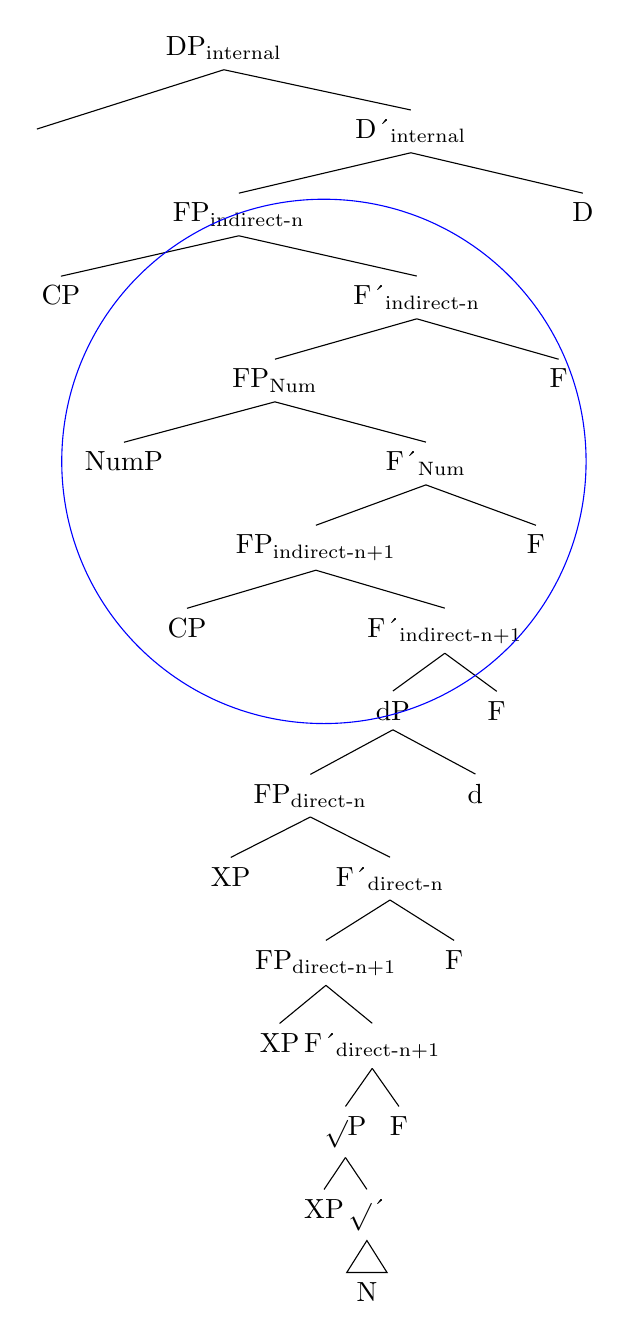
\begin{tikzpicture}[baseline=0pt, remember picture]
\tikzset{level distance=30pt, sibling distance=-5pt}
 \Tree [.DP\textsubscript{internal} {} [.D´\textsubscript{internal} [. \node (indirect1) {FP\textsubscript{indirect-n}}; CP [.\node (indirect0) {F´\textsubscript{indirect-n}}; [.FP\textsubscript{Num} NumP [.F´\textsubscript{Num} [.FP\textsubscript{indirect-n+1} \node (indirect3) {CP}; [. \node (indirect2) {F´\textsubscript{indirect-n+1}}; [.dP [.FP\textsubscript{direct-n} XP [.F´\textsubscript{direct-n} [.FP\textsubscript{direct-n+1} XP [.F´\textsubscript{direct-n+1} [.$\sqrt{}$P XP [.$\sqrt{}$´ \edge[roof]; N ] ] F ] ] F ] ] d ] F ] ] F ] ] F ] ] D ] ]
 \node[draw,circle,fit= (indirect0) (indirect3) ] [color=blue] {};
\end{tikzpicture}

 \caption{Structure of the Indirect Domain in Japanese}
 \label{fig:Structure of the Indirect Domain in Japanese1}
\end{figure}


The indirect domain is structurally higher than the direct domain and contains a projection for numerals. Japanese provides further evidence for this as direct-only modifiers are generally disallowed from a position to the left of numerals, as also argued in \citet{ayano:2010:revisiting, watanabe:2017:attributive}, highlighting that numerals are situated within the indirect domain. %\is{numerals}

\newpage

\ex. \ag. San-nin-no furu-i yūjin-ga ki-ta.\\
three-\textsc{cl-no} long.time-\textsc{i} friend-\textsc{nom} come-\textsc{pst}\\
`Three long-time friends came.' \hfill \citep[106]{ayano:2010:revisiting}
\bg. *Furu-i san-nin-no yūjin-ga ki-ta.\\
long.time-\textsc{i} three-\textsc{cl-no} friend-\textsc{nom} come-\textsc{pst}\\

Furthermore, there is no evidence that Japanese head-external relative clauses do come in different sizes, for instance full and reduced, or CP and IP/vP (see Chapter \ref{size,indirect}). Instead, they are unequivocally CPs. That means that, parallel to the situation in the direct domain, there are no dedicated functional projections for indirect modifiers in the indirect domain either, in this case based on different sizes. This correctly predicts that relative clauses can freely occur to the left or to the right of numerals in linear order. As confirmed through speaker’s judgment for \ref{patichapter2}, in out-of-the-blue contexts, both orders of relative clause and numeral are equally possible.

\ex. \label{patichapter2} \ag. [pātī-de at-ta [futari-no josei]]\\
party-\textsc{loc} meet-\textsc{pst} two-\textsc{no} woman \label{pati1}\\
\bg. [futari-no [pātī-de at-ta josei]]\\
two-\textsc{no} party-\textsc{loc} meet-\textsc{pst} woman\\
`the two women who I met at a party' \label{pati2}

Corpus data and speaker judgments of diverse examples reported in Chapter \ref{complexity} confirm this observation and the assumption that available projections are situated above and below the projection hosting numerals, which do not correlate with the structural size of relative clauses.

Hence, the two orders in \Ref{patichapter2} are attributable to two different positions the relative clause can occupy, the specifier of a functional projection above or below FP\textsubscript{Num}. I indicate this below with the two possible options marked in gray. %\is{indirect modification}

\newpage

\ex. \begin{tikzpicture}[baseline=0pt, remember picture]
\tikzset{level distance=25pt, sibling distance=5pt}
\Tree [.DP\textsubscript{internal} {} [.D´\textsubscript{internal} [.FP\textsubscript{indirect} [.CP \edge[roof]; {\textcolor{mygray}{pātī-de at-ta}} ] [.F´\textsubscript{indirect} [.FP\textsubscript{Num} [.NumP \edge[roof]; {futari-no} ] [.F´\textsubscript{Num} [.FP\textsubscript{indirect} [.CP \edge[roof]; {\textcolor{mygray}{pātī-de at-ta}} ] [.F´\textsubscript{indirect} [.... [.NP \edge[roof]; {josei} ] {} ] F ] ] F ] ] F ] ] D ] ]
\end{tikzpicture}

There is a syntax-external factor that influences the choice of speakers to place the relative clause in a specific position, namely to the left of the numeral, showing that their position is not entirely arbitrary. This factor is \textit{complexity}, understood in this book both syntactically and prosodically. Syntactic complexity reflects the amount of syntactic material. Prosodic complexity, descriptively speaking, reflects length (\citealt{hawkins:2007:efficiency}; see Chapter \ref{complexity}). An increase in complexity can be achieved, for example, when the verbal or adjectival predicate within a relative clause co-occurs with an overt subject argument, or when it is modified by a degree adverb. %\is{complexity}

That an increase in complexity causes relative clauses to be preferred in a position to the left of numerals is illustrated in the DP in \ref{doresuutsukushikattachap3}, which contains a numeral and a relative clause. This relative clause is adjectival in nature and exhibits an overt subject. Furthermore, the adjective is inflected for past. Most speakers I consulted clearly prefer the position of the relative clause to the left of the numeral over the reversed order. There is certain diversity in speaker judgments, although speakers either accept both orders or prefer the one with the relative clause on the left. The dispreferred order, with lower naturalness according to speakers, is indicated with the symbol `\#’.

\ex. \label{doresuutsukushikattachap3} \ag. [doresu-ga utsukushi-k-at-ta [futari-no josei]]\\
dress-\textsc{nom} beautiful-\textsc{pred-cop-pst} two-\textsc{no} woman \label{doresu1}\\
\bg. \#[futari-no [doresu-ga utsukushi-k-at-ta josei]]\\
two-\textsc{no} dress-\textsc{nom} beautiful-\textsc{pred-cop-pst} woman\\
`the two women whose dresses were beautiful'

This fact is thus suggestive of movement of the relative clause from a functional projection below FP\textsubscript{Num} to a projection above in an individual fashion as depicted below.

%\newpage

\ex. \ag. [doresu-ga utsukushi-katta [futari-no josei]]\\
dress-\textsc{nom} beautiful-\textsc{pst} two-two-\textsc{no} woman (= \ref{doresu1})\\
\b. \hspace{-2cm} 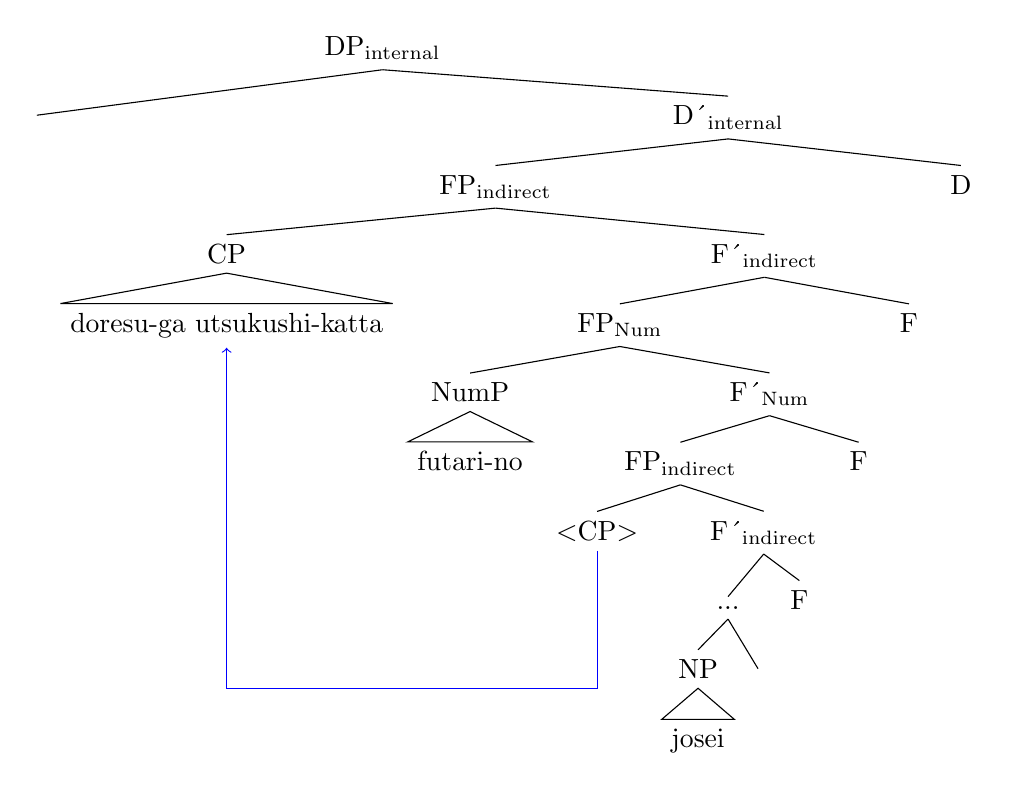
\begin{tikzpicture}[baseline=0pt, remember picture]
\tikzset{level distance=25pt, sibling distance=5pt}
\Tree [.DP\textsubscript{internal} {} [.D´\textsubscript{internal} [.FP\textsubscript{indirect} [.CP \edge[roof]; \node (cp1) {doresu-ga utsukushi-katta}; ] [.F´\textsubscript{indirect} [.FP\textsubscript{Num} [.NumP \edge[roof]; {futari-no} ] [.F´\textsubscript{Num} [.FP\textsubscript{indirect} \node (cp2) {$<$CP$>$}; [.F´\textsubscript{indirect} [.... [.NP \edge[roof]; {josei} ] {} ] F ] ] F ] ] F ] ] D ] ]
\draw [color=blue][->] (cp2) |- +(0,-2) -| (cp1);
\end{tikzpicture}

Keeping the system simple and consistent, I assume that all (but only restrictive, see Chapter \ref{RC LP}), relative clauses in Japanese merge in a position below numerals, but can potentially move up to a position above, or also to the left periphery (see below). This assumption predicts that such movement operations are open potentially to all relative clauses \citep{kim:2019:syntax}. The more complex a relative clause is, the more likely it is to move to a higher position. This point is illustrated with more data and further discussed in Chapter \ref{complexity}, especially in Chapter \ref{RC discussion}, and see Fn. \ref{footnote complexity} where I outline why it fares better than its alternatives.

\subsection{The left periphery} \label{externaldp}

The DP-external domain, also referred to as the left periphery, is not the main focus of this study, but will be investigated briefly here since Japanese provides evidence for this domain. Notably, this area is postulated, and investigated with regards to several languages in the works of \citet{giusti:1996:is, dimitrova:1998:fragments, ihsane:2001:specific, aboh:2004:topic, aboh:2006:when, roca:2009:left, bastos:2011:info, giusti:2016:latin, roehrs:2019:left, roehrs:2025:DP, kim:2019:syntax}, for the integration in formal frameworks see \citet{laenzlinger:2011:elements} and \citet{grohmann:2003:prolific}. I will discuss every type of modifier attested in this area in Japanese and argue that there are many insights and incentives for future research regarding this peripheral area to be gained by looking at this language. %\is{left periphery}

\subsubsection{Demonstratives}

Japanese lacks articles, but has demonstratives. They can be simple, the standard ones being \textit{kono} `this’ and its counterparts, which only vary in deixis - and complex, such as \textit{koko-no} `the (one) here’ or \textit{korekara-no} `the one from now on’. I adopt the standard assumption of demonstratives as maximal projections \citep{laenzlinger:2005:french, laenzlinger:2011:elements, kim:2019:syntax}, but in Japanese, they are specifiers, not heads \citep{kuno:1973:structure, kuroda:1992:japanese}. An analysis as heads would violate the strict head-finality of Japanese since demonstratives never occur postnominally. %\is{demonstratives}

Demonstratives first merge as specifiers of the DP projection heading the internal domain. I follow previous authors \citep{laenzlinger:2011:elements, kim:2019:syntax} and assume that they can optionally move to the specifier position of the DP heading the DP-external domain if modifiers have moved to a position in the left periphery. I adopt the simplistic notions DP\textsubscript{internal} for the lower and DP\textsubscript{external} for the higher DP projection. since there is no obvious semantic or pragmatic difference whether demonstratives occur in the lower or higher position.

\subsubsection{Quantificational modifiers} \label{quantificational modifiers}

The DP-external domain contains a projection for quantifiers, or more precisely \textit{quantificational modifiers}, which will be labeled FP\textsubscript{QUANTITY}. Most quantificational modifiers in Japanese are \textsc{no}-modifiers, including \textit{takusan-no} `a lot’, \textit{kazukazu-no} `many', \textit{subete-no} `all' and \textit{amari-no} `few' as well as \textit{ōku-no} `many’.\footnote{Quantification can also be expressed via Sino-Japanese prefixes such as \textit{kaku}- `each, every' or \textit{zen}- `all’, which are simply juxtaposed to the head noun. \textit{Bōdai-na} `giant, huge’ is a \textit{na}-adjective. I am grateful to Ken Hiraiwa for reminding me of this.}

Cross-linguistically, there is a tendency for quantificational modifiers to appear rather high in the DP. In German, they have to precede (ambiguous) qualitative \ref{vielestrenge} and also direct adjectives \ref{vielefruhere}. This behavior of German quantifiers is verified in the corpus study reported in \citet[378]{trost:2006:das}, and see also \citet{eichinger:1991:ganz}. %\is{quantifiers}

\ex. \label{vielestrenge} German
 \ag. viele strenge Präsidenten\\
many strict presidents\\
`many strict presidents’
\bg. *strenge viele Präsidenten\\
strict many presidents\\

\newpage

\ex. \label{vielefruhere} German
 \ag. viele frühere Präsidenten\\
many former presidents\\
`many former presidents’
\bg. *frühere viele Präsidenten\\
former many presidents\\

This generalization partly holds in Japanese: When quantificational modifiers and direct-only modifiers co-occur, the quantifier typically occurs first, the other order being degraded.

\ex. quantificational modifier $\succ$ non-intersective modifier
\ag. \textbf{ōku-no} shōrai-no purosakkāsenshu\\
many-\textsc{no} future-\textsc{no} pro.soccer.player\\
`many future professional soccer players’
\bg. *shōrai-no \textbf{ōku-no} purosakkāsenshu\\
future-\textsc{no} many-\textsc{no} pro.soccer.player'\\

\ex. quantificational $\succ$ relational modifier
\ag. \textbf{takusan-no} komugi-no pan\\
a.lot-\textsc{no} wheat-\textsc{no} bread\\
`many wheat(-en) (pieces of) bread’ \label{takusankomugi}
\bg. ??komugi-no \textbf{takusan-no} pan\\
wheat-\textsc{no} a.lot-\textsc{no} bread\\

Importantly, quantifiers in Japanese do not only readily co-occur with demonstratives, when they do, they can occur before and after them. %\is{demonstratives, quantifiers}

\ex. \ag. ano \textbf{kazukazu-no} mondai\\
that many-\textsc{no} problem\\
\bg. \textbf{kazukazu-no} ano mondai\\
many-\textsc{no} that problem\\
`those many problems’

\ex. \ag. ano \textbf{takusan-no} hon\\
that a.lot-\textsc{no} book\\
\bg. \textbf{takusan-no} ano hon\\
a.lot-\textsc{no} that book\\
`those many books’

This is a significant deviation to, for example, English where quantifiers can only co-occur with demonstratives or articles in certain contexts in the first place, for example in \textit{those many students} or \textit{the few students who attended the lecture}, but crucially only in this order, never in the order \textit{quantifier} $\succ$ \textit{demonstrative}.

\ex. *many those students

From this, I conclude that quantificational modifiers in Japanese are generally situated in the left periphery. The surface order \textit{demonstrative} $\succ$ \textit{quantifier} is a result of the demonstrative having moved from the internal DP to Spec, DP\textsubscript{external}, similar to what \citet{laenzlinger:2005:french, laenzlinger:2011:elements} argues for French. That this happens regularly in Japanese, is corroborated since speaker still find this order a bit more natural.

The question remains whether quantifiers actually move to the left periphery or base-generate there (cf. \citealt{kim:2019:syntax}). There is good evidence that they originate lower, probably inside the direct domain. Note that many quantificational modifiers in Japanese are exclusively used attributively, while for others this is the prototypical use. In fact, all quantificational modifiers attested in the data set are sorted in group 5, the group for direct modifiers. While some are truly exclusively direct, others, such as \textit{takusan-no} `a lot’, could in principle have a predicative source, but given the ratio of 14:1 towards attributive use (4048 attributive, 172 predicative occurrences), a categorization as a prototypical attributive modifier is justified (for details see \citealt{kohlich:2023:suppl}). Direct-only quantificational modifiers, those which are impossible as predicates, include \textit{kazukazu-no} `many’, \textit{shuju-no} `various’ and \textit{amata-no} `a lot, many’ as illustrated below.

\ex. \ag. Kare-wa kazukazu-no shō-wo tot-ta.\\
he-\textsc{top} many-\textsc{no} prize-\textsc{acc} take-\textsc{pst}\\
`He received many prizes.’
\bg. *Kare-ga tot-ta shō-wa kazukazu-desu.\\
he-\textsc{nom} take-\textsc{pst} prize-\textsc{top} many-\textsc{cop.pol}\\
(`The prizes he received were many.’)

%\newpage

\ex. \ag. Kare-wa shuju-no / amata-no shikaku-wo mot-te-i-ru.\\
he-\textsc{top} various-\textsc{no} / many-\textsc{no} qualification-\textsc{acc} have-\textsc{ger}-be-\textsc{prs}\\
`He has various / many qualifications.’
\bg. *Kare-ga mot-te-i-ru shikaku-wa shuju-desu / amata-desu.\\
he-\textsc{nom} have-\textsc{ger}-be-\textsc{prs} qualification-\textsc{top} various-\textsc{cop.pol} / many-\textsc{cop.pol}\\
(`The qualifications he has are various / many.’)

Based on these facts, I conclude that quantificational modifiers are base-generated in the direct domain, but have to move to the left periphery. I tentatively assume that this movement happens to check [+quantificational] features, in line with \citet{kim:2019:syntax}, and that they move to a dedicated position, call it FP\textsubscript{QUANTITY}, although more concrete evidence is desirable. The derivation looks as follows.

\newpage

\ex. \ag. takusan-no komugi-no pan\\
a.lot-\textsc{no} wheat-\textsc{no} bread\\
`many wheat(-en) (pieces of) bread’ (= \ref{takusankomugi})
\b. \hspace{-2cm} 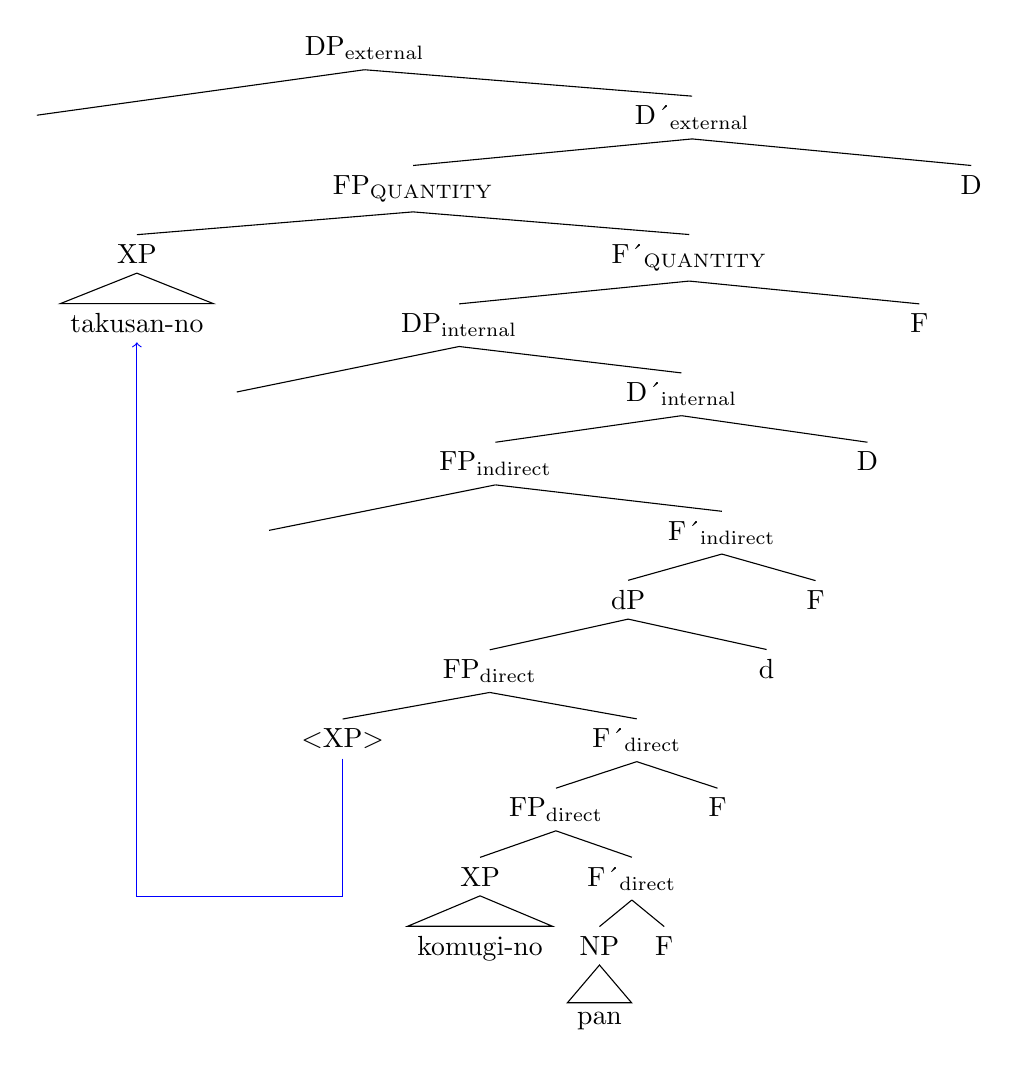
\begin{tikzpicture}[baseline=0pt, remember picture]
\tikzset{level distance=25pt, sibling distance=5pt}
\Tree [.DP\textsubscript{external} {} [.D´\textsubscript{external} [.FP\textsubscript{QUANTITY} [.XP \edge[roof]; \node (isha1) {takusan-no}; ] [.F´\textsubscript{QUANTITY} [.DP\textsubscript{internal} {} [.D´\textsubscript{internal} [.FP\textsubscript{indirect} {} [.F´\textsubscript{indirect} [.dP [.FP\textsubscript{direct} \node (isha2) {$<$XP$>$}; [.F´\textsubscript{direct} [.FP\textsubscript{direct} [.XP \edge[roof]; komugi-no ] [.F´\textsubscript{direct} [.NP \edge[roof]; {pan} ] F ] ] F ] ] d ] F ] ] D ] ] F ] ] D ] ]
\draw [color=blue][->] (isha2) |- +(0,-2) -| (isha1);
\end{tikzpicture}

\subsubsection{Non-restrictive and restrictive relative clauses} \label{RC LP}

Another argument in favor of a split-DP structure is the fact that a certain class of relative clauses in Japanese obligatorily precedes demonstratives, namely those that are non-restrictive. First, note that all relative clauses \textit{can} readily precede demonstratives in Japanese. This means that when no context is provided, a relative clause in this position is ambiguous and can be interpreted non-restrictively or restrictively, as depicted in \ref{resrc}.\footnote{The initial observation goes back to \citet{kamio:1977:restrictive}, who pointed out a paradigmatic difference between non-restrictive pre-demonstrative relative clauses and restrictive post-demonstrative relative clauses. \citet{ishizuka:2008:RC}, whom this section follows, has discussed in detail that pre-demonstrative relative clauses are ambiguous.} %\is{relative clauses}

\newpage

\exg. [Sakunen isha-ni nat-ta [sono musuko-ga]] kekkon-shi-ta.\\
last.year doctor-\textsc{loc} become-\textsc{pst} that son-\textsc{nom} marriage-do-\textsc{pst}\\
1. $\approx$ `That son who became a doctor last year got married.’ (restrictive) \\
2. $\approx$ `That son, who happened to become a doctor last year, got married.' (non-restrictive) \\ \null \hfill \citep[4, 5]{ishizuka:2008:RC} \label{resrc}

However, when the same relative clause follows the demonstrative, it can \textit{only} be interpreted restrictively. Establishing a context that forces a non-restrictive interpretation leads to ungrammaticality as depicted in \ref{only resrc}, see \citet{ishizuka:2008:RC}. %\is{non-restrictive relative clauses}

\exg. *Ito-san-ni-wa musuko-ga hitori i-ru. [Sono [sakunen isha-ni nat-ta] musuko-ga] kekkon-shi-ta.\\
Ito-Mr./Mrs.-\textsc{loc-top} son-\textsc{nom} one be-\textsc{prs} that last.year doctor-\textsc{loc} become-\textsc{pst} son-\textsc{nom} marriage-do-\textsc{pst}\\
(`Mr./Mrs. Ito has one son. That son, who happened to become a doctor last year, got married.’) \\ \null \hfill \citep[5]{ishizuka:2008:RC} \label{only resrc}

In other words, in Japanese, only restrictive relative clauses are allowed after demonstratives, non-restrictive relative clauses are confined to a position in the left periphery. Following \citet{ishizuka:2008:RC} and \citet{cinque:2008:two}, I take this type of relative clause to be base-generated in a dedicated projection in the DP-external domain. In this position, they are outside the scope of the demonstrative, which accounts for the lack of scope effects and the obligatorily non-restrictive interpretation. This proposal is based on \citet{kim:2019:syntax}, who introduces a projection for non-integrated, \textit{supplementary}, relative clauses (Spec, SpplP) in Korean. The difference is that, in Japanese, non-restrictive relative clauses obligatorily merge outside the internal DP, whereas in Korean a certain type of non-restrictive relative clause can also merge lower.\footnote{\label{footnote German RC} A reviewer asks what the basis for the difference between Japanese and Korean regarding the position of non-restrictive relative clauses is. At this point, I cannot give a definitive answer. Languages seem to differ substantially as to which types of relative clauses they allow in the left periphery (if any). Whereas in Japanese, non-restrictive relative clauses have to occur in the left periphery, and in Korean a subtype of non-restrictive relative clauses, namely supplementary ones have to, German only allows restrictive relative clauses in the nominal left periphery \citep{kohlich:2026:ms}. Forcing a non-restrictive interpretation, by means of the adverb \textit{übrigens} `by the way', leads to degraded results (see also \citealt{bhatt:1990:syntaktisch, roehrs:2019:left}).

\par

\exg. ??Der (übrigens) Bass singt, der Opernsänger hat für seine Vorstellung einen Preis gewonnen. (German)\\
the by.the.way bass sings the opera.singer has for his performance a prize won\\
`The opera singer, who (by the way) sings bass, has won a prize for his performance.’

}  The relevant position is depicted in the tree below.

\newpage

 \ex. \ag. isha-ni nat-ta sono musuko (non-restrictive)\\
doctor-\textsc{loc} become-\textsc{pst} that son\\
\b. 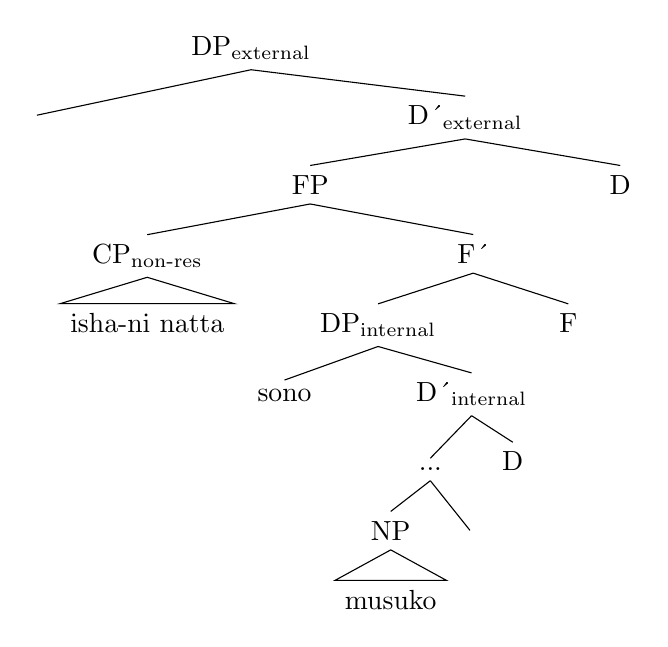
\begin{tikzpicture}[baseline=0pt, remember picture]
\tikzset{level distance=25pt, sibling distance=5pt}
\Tree [.DP\textsubscript{external} {} [.D´\textsubscript{external} [.FP [.CP\textsubscript{non-res} \edge[roof]; {isha-ni natta} ] [.F´ [.DP\textsubscript{internal} sono [.D´\textsubscript{internal} [.... [.NP \edge[roof]; musuko ] {} ] D ] ] F ] ] D ] ]
\end{tikzpicture}

Restrictive relative clauses, on the other hand, are base-generated DP-internally, as outlined in the preceding section, presumably below NumP. Their restrictiveness is expected being under the scope of D. In addition to individual movement within the indirect domain to a position above FP\textsubscript{Num}, I argue that restrictive relative clauses can even cross the internal DP border as depicted below.\footnote{According to \citet{ishizuka:2008:RC}, scope effects are retained through reconstruction and the moved relative clause keeps its restrictive interpretation. It does not become entirely clear how reconstruction works in Ishizuka's system and readers are referred to her proposal. See also footnote \ref{footnote ishizuka} in Chapter \ref{RCs above dem}.}

\newpage

 \ex. \ag. isha-ni nat-ta sono musuko (restrictive)\\
doctor-\textsc{loc} become-\textsc{pst} that son\\
 \b. 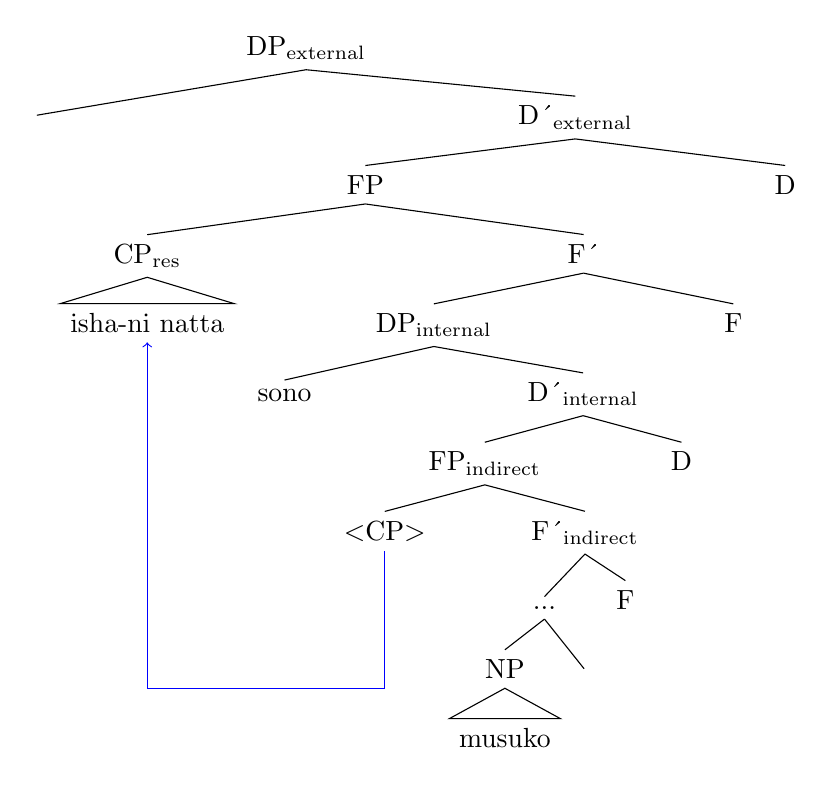
\begin{tikzpicture}[baseline=0pt, remember picture]
\tikzset{level distance=25pt, sibling distance=5pt}
\Tree [.DP\textsubscript{external} {} [.D´\textsubscript{external} [.FP [.CP\textsubscript{res} \edge[roof]; \node (isha1) {isha-ni natta}; ] [.F´ [.DP\textsubscript{internal} sono [.D´\textsubscript{internal} [.FP\textsubscript{indirect} \node (isha2) {$<$CP$>$}; [.F´\textsubscript{indirect} [.... [.NP \edge[roof]; musuko ] {} ] F ] ] D ] ] F ] ] D ] ]
\draw [color=blue][->] (isha2) |- +(0,-2) -| (isha1);
\end{tikzpicture}

What about non-restrictive relative clauses to the right of demonstratives then? Given the fact that they, as I argued, merge in the DP-external domain, the surface order is the result of movement by the demonstrative from the DP-internal to the DP-external domain across the non-restrictive relative clause in the left periphery. This predicts, correctly, that non-restrictive relative clauses are allowed below demonstratives.

\subsubsection{Direct modifiers }

Direct modifiers can also productively appear above demonstratives, given the right circumstances, but seemingly in free alternation. %\is{direct modifiers}

\ex. \ag. kono izen-no rūru\\
this former-\textsc{no} rule\\
\bg. izen-no kono rūru\\
former-\textsc{no} this rule\\
`this former rule’

From this, I conclude that direct modifiers have the option to leave the direct domain and move to the left periphery as well, in a similar fashion to quantificational modifiers. Importantly, they are not required to do so and this movement is optional.

\newpage

\ex. 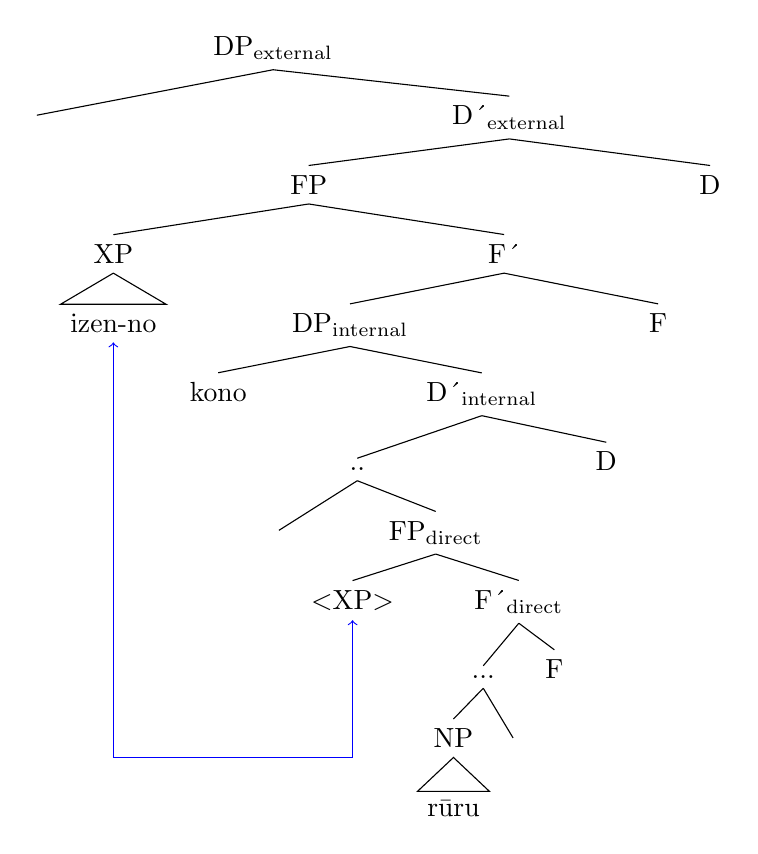
\begin{tikzpicture}[baseline=0pt, remember picture]
\tikzset{level distance=25pt, sibling distance=5pt}
\Tree [.DP\textsubscript{external} {} [.D´\textsubscript{external} [.FP [.XP \edge[roof]; \node (isha1) {izen-no}; ] [.F´ [.DP\textsubscript{internal} kono [.D´\textsubscript{internal} [... {} [.FP\textsubscript{direct} \node (isha2) {$<$XP$>$}; [.F´\textsubscript{direct} [.... [.NP \edge[roof]; rūru ] {} ] F ] ] ] D ] ] F ] ] D ] ]
\draw [color=blue][<->] (isha2) |- +(0,-2) -| (isha1);
\end{tikzpicture}

\subsubsection{A discussion on focused modifiers} \label{focus,japanese}

Focused modifiers and their connection to the left periphery, both within the DP and the clause, make up a rich and controversial research area. The high occurrence of modifiers with a focus (and topic) interpretation, in some cases above D-elements, is one of the main motivations for the split-DP hypothesis (\citealt{kiss:1998:identificational, kiss:2007:topic, giusti:1996:is, dimitrova:1998:fragments, ihsane:2001:specific, laenzlinger:2005:french, kim:2019:syntax} a. o.; cf. \citealt[140–151]{alex:2007:nounphrase} for discussion). The classical observation goes back to \citet{giusti:1996:is, dimitrova:1998:fragments}, who point out that adjectives in Albanian, which naturally occur postnominally and are marked when they appear prenominally, can reach a position above demonstratives, analyzed as FocP, via A´-movement for focus reasons leading to DPs such as \ref{albanian}. %\is{focus} %\is{albanian}

\exg. TJOTR-a grua e bukur (Albanian)\\
other-the woman \textsc{det} nice\\
`the other nice woman' \\ \null \hfill \citep[113]{giusti:1996:is} \label{albanian}

\citet{ihsane:2001:specific} show that a focus interpretation, with focal stress is also available to numerals and possessors in certain languages and, again, focus movement is triggered. In Hungarian, this, in turn, forces the article to subsequently move to a higher position, to check the feature [+specific], according to the authors. This position corresponds to DP\textsubscript{external} proposed here, whereas the numeral with the focus interpretation in \ref{hungarianaz} is in DP\textsubscript{internal}. %\is{hungarian}

\ex. \label{hungarianaz} \ag. az EGY könyv (Hungarian)\\
the ONE book \\
\bg. *EGY az könyv\\
ONE the book \\ \null \hfill \citep[48]{ihsane:2001:specific}\\

\citet[ch. 6.7]{kim:2019:syntax} argues that a focus projection is universal and that exactly one FocP should be assumed in the left periphery (see also \citet{giusti:2016:latin, roehrs:2019:left}). This position arguably is below FP\textsubscript{QUANTITY} accounting for the ordering in \ref{unskillful}.

\ex. \label{unskillful} \a. most UNSKILLFUL doctors \null \hfill \citep[137]{kim:2019:syntax}
\b. *UNSKILLFUL most doctors

Focus movement has also been invoked in order to account for non-canonical orders of adjectives such as \textit{RED big book} (see also \citealt{svenonius:2008:position}). Arguably, the focused adjective in such cases has move to the specifier of a focus projection, which, however, is below the DP projection in English. %\is{focus}

\exi. [DP the [FocP RED [FP\textsubscript{indirect} ... [FP\textsc{dimension} big [FP\textsc{color} $<$red$>$ ... [NP book ]]]]]] %\newpage

However, in most languages, modifiers can also receive in-situ focus \citep[191]{kim:2019:syntax} suggesting the absence of an EPP feature of FocP in such cases.

\ex. I need a big RED book, not a big BLUE one.

Japanese is a language (similar to, for instance, Gungbe, cf. \citealt{aboh:2004:topic}) which exhibits \textit{focus sensitive particles}. The prototypical topic marker -\textsc{wa} can also acquire a focus function \ref{focuswa}, other focus sensitive particles are -\textsc{dake} `only' or -\textsc{sae} `even’ \ref{focusdake} (\citealt{tomioka:2009:contrastive, tomioka:2016:infor, vermeulen:2007:jap, vermeulen:2012:info}, see also Chapter \ref{focusrc}).

%\newpage

\exg. [Nihongo-wo shanai-de-\textbf{wa} tsuka-u] gaikokujin\\
Japanese-\textsc{acc} office-\textsc{loc}-\textsc{foc} use-\textsc{prs} foreigner\\
`a foreigner who uses Japanese only in the office’ \\ \null \hfill \citep[93]{akaso:2011:on} \label{focuswa}

\newpage

\exg. Taro-dake/mo/sae ano mise-de nihongo-no shōsetu-wo kat-ta.\\
Taro-only/also/even that shop-\textsc{loc} Japanese-\textsc{mod} novel-\textsc{acc} buy-\textsc{pst}\\
`Only/Also/Even Taro bought Japanese novels at that shop.'  \\ \null \hfill \citep[195]{vermeulen:2012:info} \label{focusdake}

These elements mark instances of clausal focus and cannot be freely combined with DP-internal constituents in order to put focus, for instance, on numerals, shown below for \textsc{dake} `only’.

\exg. *Ni-satsu-dake-no hon-wo kat-ta. \label{futatsu}\\
two-\textsc{cl}-only-\textsc{no} book-\textsc{acc} buy-\textsc{pst}\\
(`I bought only two books.’)

The intended meaning can be expressed if the quantifier is used as an adverbial modifier within the verbal domain, as in \ref{nisatsudake}. In this case, it can optionally be left-dislocated to a clause-initial position. Clearly, it is not part of the DP, since it does not occur with \textsc{no}, or any other form of the linker (see bleow), which we would expect if it was a nominal modifier. %(quantifier floating)

\exg. Ni-satsu-dake, hon-wo kat-ta.\\
two-\textsc{cl}-only, book-\textsc{acc} buy-\textsc{acc}\\
`I bought only two books.’ (Lit. `Two only, I bought books.’) \label{nisatsudake}

The focus sensitive particle \textsc{dake} can, however, attach to a numeral classifier and then occur DP-internally as shown in \ref{himitsu} where it attaches to \textit{futari} `two.people’, a suppletive form of the classifier for people -\textit{nin} and the number 2. That the focus sensitive particle is part of the DP becomes clear as \textsc{no} obligatorily occurs. %\is{focus}

%\newpage

\exg. futari-dake-no himitsu-ni shi-te-ok-ō to [...]\\
two.people-only-\textsc{no} secret-\textsc{dat} do-\textsc{ger}-prepare-\textsc{epis} \textsc{comp}\\
`to make it a secret shared only by two [...].’ (Lit. `a two-person only secret..’)\footnote{Nakanishi, Rei (2003): Yotō. Tokyo: Shinchōsha, via BCCWJ, 2023/11/09.} \label{himitsu}

Crucially, \textsc{dake} does not add focus to the noun \textit{himitsu} `secret’, but to the numeral \textit{futari} `two people’, so what is focused is the amount of people. In any case, this example shows that focus is possible DP-internally which suggests the existence of FocP in Japanese (see Chapters \ref{focusrc} and \ref{focusincp}).

Furthermore, in contrast to the Hungarian example presented in \ref{hungarianaz}, Japanese allows additional modifiers to precede focused numeral classifiers marked by \textsc{dake}, although this might not be the default order. \ref{sannindake} shows that both orders of modifiers are fine.\footnote{I am grateful to Ken Hiraiwa for bringing all these facts to my attention.}

%\newpage

\ex. \label{sannindake} \ag. san-nin-dake-no kura-i himitsu\\
three-person-\textsc{cl}-only-\textsc{no} dark-\textsc{i} secret\\
\bg. kura-i san-nin-dake-no himitsu\\
dark-\textsc{i} three-person-\textsc{cl}-only-\textsc{no} secret\\
`a dark secret shared by only three people’

These facts indicate that there seems to be no requirement for focused modifiers to occur in the left periphery, suggesting the absence of a requirement for movement. This is backed up by evidence from the position of prosodically focused lexical modifiers. Although being a pitch-accent language, Japanese can express focus via accentuation and prosody \citep{beckman:1986:intonational, hiraiwa:2012:syntactic, tomioka:2009:contrastive}. Modifiers with prosodic focus can occur in a higher, DP-initial, position, but they can also remain in-situ. In \ref{akamaruchap3}, both answers are possible to the preceding question, emphasizing \textit{maru-i} `round’.\footnote{Japanese also bears an interesting similarity to Latin. Although this language had a comparatively free word order and modifiers on both side of the noun, adjectives were consistently placed more often in a position to the left of the noun if used contrastively as shown by \citet{devine:2006:latin}. However, adjectives are not obligatorily placed in this position. An even more intriguing parallel to Japanese is that ``unfocused adjectives can raise to the left of the head as well as focused adjectives’’ \citep[409]{devine:2006:latin}, exactly paralleling the case with scrambled unfocused adjectives in the left periphery in Japanese.} %\is{adjective ordering restrictions}

%\newpage

\ex. \label{akamaruchap3} \ag. [Aka-i maru-i tēburu] ka, [aka-i shikaku-i tēburu] dotchi-wo kat-ta no?\\
red-\textsc{i} round-\textsc{i} table \textsc{q} red-\textsc{i} square-\textsc{i} table which-\textsc{acc} buy-\textsc{pst} \textsc{q}\\
`Did you buy the red round table or the red square table?'
\bg. Aka-i MARU-I tēburu-wo kat-ta yo.\\
red-\textsc{i} round-\textsc{i} table-\textsc{acc} buy-\textsc{pst} \textsc{sfp}\\
`I bought the red ROUND table.’
\cg. MARU-I aka-i tēburu-wo kat-ta yo.\\
round-\textsc{i} red-\textsc{i} table-\textsc{acc} buy-\textsc{pst} \textsc{sfp}\\
`I bought the ROUND red table.’

Crucially, prosodic stress is in some instances not even enough to allow modifiers to move to a higher position. Recall from \ref{directrcchap3}, given in Chapter \ref{internaldirect}, that direct modifiers cannot precede relative clauses. This observation still holds if the non-intersective modifier \textit{shōrai-no} `future' is focused, meaning it must remain in-situ and cannot cross the indirect domain.

\newpage

\ex. \ag. Kare-wa [ōku-no kurabu-ga chūmoku-shi-te-i-ru [\textbf{SHŌRAI-no} purosakkāsenshu]]-desu.\\
he-\textsc{top} numerous-\textsc{no} club-\textsc{nom} pay.attention-do-\textsc{ger}-be-\textsc{prs} future-\textsc{no} pro.soccer.player-\textsc{cop.pol}\\
`He is a FUTURE professional soccer player whom many clubs pay attention to.’
\bg. *Kare-wa [\textbf{SHŌRAI-no} [ōku-no kurabu-ga chūmoku-shi-te-i-ru purosakkāsenshu]]-desu.\\
\textsc{top} future-\textsc{no} numerous-\textsc{no} club-\textsc{nom} pay.attention-do-\textsc{ger}-be-\textsc{prs} pro.soccer.player-\textsc{cop.pol}\\

Note that movement to a non-canonical position is available in Japanese as the co-occurrence with demonstratives has shown. Such a non-canonical position is presumably also available for some direct-only modifiers in English, as shown below.

\ex. I want to meet a FORMER handsome president, not a current one.

Final evidence for the absence of an EPP-feature for FocP in Japanese comes from superlatives, another category of modifiers that has been argued to obligatorily occur within the left periphery \citep{cinque:2010:adj, cinque:2023:linearization}. In English, if an adjective in superlative co-occurs with a numeral, moving the superlatives across the numeral is necessary (cf. \citealt[11]{cinque:2023:linearization} and Guglielmo Cinque p.c.). %\is{focus movement}

\ex. \a. the blackest two dogs (that I've ever seen)
\b. ??the two blackest dogs

However, this is not the case in Japanese. On the contrary, both orders are fine.

\ex. \ag. ichi-ban kuro-i ni-hiki-no inu\\
number-one black-\textsc{i} two-\textsc{cl-no} dog\\
`the blackest two dogs'
\bg. ni-hiki-no ichi-ban kuro-i inu\\
two-\textsc{cl-no} number-one black-\textsc{i} dog\\
`the two blackest dogs'

To summarize, focused modifiers in Japanese are not required, and sometimes not allowed, to move to the left periphery, although, in most cases, they seem to be able to allow such movement operations. From this, I conclude that the left periphery contains a focus projection, which has been proven empirically adequate and necessary in cross-linguistic perspective, but that, in Japanese, this projection simply lacks an EPP feature, and its Spec position can remain empty.

\section{The Internal structure of modifiers} \label{internalstructure}

In this section, I develop an account for the internal structure of Japanese modifiers, a crucial aspect that has been missing in the discussion so far. This concerns both, the monomoraic elements co-occurring with direct and ambiguous modifiers, as well as the complex internal structures available to indirect modifiers. In cartographic accounts, the internal structure of modifiers and the general DP structure are typically treated orthogonally. Te account proposed in the following will yield new insights that further enrich the general understanding of the DP.

\subsection{Introduction}

In this section, I focus especially on the monomoraic elements \textsc{no}, \textsc{i} or \textsc{na} which always co-occur with non-verbal modifiers in Japanese in attributive position if those express non-past in positive contexts.

\ex. \ag. hisshu-*(no) yoyaku\\
urgent-\textsc{no} reservation\\
`urgent reservation’ \null \hfill \textit{no}-modifier \label{mumeino}
\bg. taka-*(i) doresu\\
expensive-\textsc{i} dress\\
`expensive dress' \null \hfill \textit{i}-adjective \label{takaimod1}
\cg. shikku-*(na) doresu\\
chic-\textsc{na} dress\\
`chic dress' \null \hfill \textit{na}-adjective \label{shikkunamod1}

Those elements cannot be analyzed as parts of the stem, since they disappear when the relevant lexemes, those which can, appear predicatively. Instead, the copula appears. A special behavior is exhibited by \textit{i}-adjectives, where the vowel \textsc{i} also appears in predicative position.\footnote{This is the reason why authors such as \citet{nishiyama:1999:adj} treat them as the same element (see Chapter \ref{copulaelements}. In this study, I propose two different analyses for \textsc{i}.}

\ex. \label{nopredicativeno} \ag. Ano haiyū-wa mumei (*no) da.\\
that actor-\textsc{top} unknown \textsc{no} \textsc{cop}\\
`That actor is unknown.’ \null \hfill \textit{no}-modifier
\bg. Ano doresu-wa taka-i.\\
that dress-\textsc{top} expensive-\textsc{i}\\
`That dress is expensive.' \null \hfill \textit{i}-adjective
\cg. Ano doresu-wa shikku (*na) da.\\
that dress-\textsc{top} chic \textsc{na} \textsc{cop}\\
`That dress is chic.' \null \hfill \textit{na}-adjective

\textsc{no} and \textsc{na} are also mutually exclusive with other forms of the copula, namely the (canonical) long forms for non-past \textsc{dearu} and past \textsc{d(e)atta}. %\is{copula}

\ex. \label{dearuno} \ag. ano mumei-dearu (*no) haiyū\\
that unknown-\textsc{cop} \textsc{no} actor\\
`that actor who is unknown' \null \hfill \textit{no}-modifier
\bg. ano shikku-dearu (*na) doresu\\
that chic-\textsc{cop} \textsc{na} dress\\
`that dress which is chic’ \null \hfill \textit{na}-adjective

Thus, the question arises how these elements should be treated. Especially, the element \textsc{no} is of interest, since, as shown in Chapter \ref{intro japanese}, it is incredibly widely distributed and appears with a variety of lexical elements with different degrees of adjectival and nominal status, as well as different functional elements. Furthermore, most direct modifiers co-occur with this element, although by far not all \textit{no}-modifiers are direct. This means an account of this recalcitrant element with enough explanatory power to either explain why it appears in so many different instances, or alternatively to reduce all these instances to one underlying function is desirable.

In this section, I will propose a unifying account of \textsc{no} as a syntactic head which licenses modification, meaning I will choose such a unifying account. This account predicts neither restrictions on different word classes nor on modification types. In the next step, this analysis will be applied to the elements \textsc{i} and \textsc{na} whose distribution is more restricted as the lexemes they co-occur with are clearly adjectives. I will then discuss why the analysis presented here fares better than alternative accounts before I outline the integration of these elements in the DP.

\subsection{A universal syntactic head}

\subsubsection{The basic idea}

I argue that \textsc{no} is the realization of a syntactic head, which I call \textbf{MOD} following \citet{rubin:1993:category, rubin:1994:mod, rubin:1996:transparent}. This head mediates modification within the DP. The basic assumptions are as follows. %\is{mod}

\ex. \a. Modifiers in Japanese must be licensed by a syntactic head in attributive position.
\b. This head can be realized overtly in Japanese. Its unspecified spell-out form is /no/.
\c. \textsc{mod} selects modifiers irrespective of modification type and word class. Whether a modifier is direct or indirect is decided in the syntax.

In this sense, \textsc{mod} belongs to the category of syntactic linkers. There are several linker architectures on the market,\footnote{For overview over linkers in the nominal, and also clausal domain, see among others \citealt{baker:2006:linkers, philip:2012:linkers, franco:2015:linkers, richards:2023:finding}.}  but I apply the rather minimalistic account of \citet{rubin:1994:mod, rubin:1996:transparent} to Japanese. Concretely, I argue that \textsc{mod} is a functional head that obligatorily selects a modifier - lexical or functional - as its complement and licenses them as modifiers \citep[36–40]{rubin:1994:mod}, itself being selected by the noun. In this sense, \textsc{mod} is the modificational counterpart of \textsc{pred}, discussed in Chapter \ref{chapter pred}.\footnote{Both elements are functional and universal. They are also historically related, as both Bowers and Rubin (and Nishiyama) worked at Cornell University.}

 A minimal representation, as \textsc{mod} is proposed in \citet{rubin:1994:mod}, looks as follows exemplified with a \textit{no}-modifier

\ex. \label{mumeimod} \ag. mumei-no haiyū\\
unknown-\textsc{mod} actor (= \ref{mumeino})\\
\b. 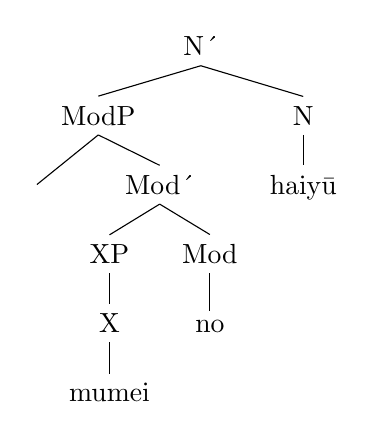
\begin{tikzpicture}[baseline=0pt, remember picture]
\tikzset{level distance=25pt, sibling distance=5pt}
 \Tree [.N´ [.ModP {} [.Mod´ [.XP [.X mumei ] ] [.Mod no ] ] ] [.N haiyū ] ]
\end{tikzpicture}

Furthermore, I argue, that this head is universal, but optionally realized, depending on the language. This sticks to the core assumptions of cartography. As languages only differ in if and how they realize lexical material mapped onto the functional structure \citep{rizzi:1997:the, shlonsky:2004:form, bortolotto:2016:RA, cinriz:2010:carto, cinriz:2016:functional}, this head might be covert in most languages (see also \citealt{richards:2023:finding}). In addition to the overt realizations of this head detected by \citet[ch. 2.2 + 2.3]{rubin:1994:mod} in Romanian, Tagalog and Mandarin, allowing a reanalysis of the element \textsc{de} in Mandarin as \textsc{mod} \citep[97–102]{rubin:1994:mod}, I propose that it is also overtly realized inside the Japanese DP.\footnote{These realizations fulfill all the characteristics expected from functional categories: They are phonologically and morphologically dependent, cannot be separated from their complements and lack semantic meaning, ``descriptive content’’ in the sense of Abney (\citeyear[65–66]{abney:1987:the}; see \citealt[34]{rubin:1994:mod}). \citet[ch. 2.2 + 2.3]{rubin:1994:mod} also analyzes the agreement systems of Russian and German as instances of \textsc{mod}. For recent discussion on German and Dutch see \citet{zeijlstra:2020:agree} and \citet{alexeyenko:2021:hff}. The \textit{ezāfe} morpheme appearing obligatorily with modifiers in Western Iranian languages including Persian and Zazaki might also be a good candidate for this analysis. See for instance \citet{toosarvandani:2014:the, franco:2015:linkers} and \citet{gn:2024:morpho} for relevant analyses and the Persian data in Chapter \ref{persiananalysis}.}

\subsubsection{Integration in The DP}

The minimal structure given above in \ref{mumeimod} of a noun phrase with \textsc{mod} selecting a modifier can be directly integrated into the cartographic DP as in \ref{anomumei}. This means what actually is embedded in the specifier position of the relevant functional projection is a modifier selected by \textsc{mod}. Following \textit{no}-modifiers, \textsc{mod} is overtly realized as /no/. Recall that \textit{mumei-no} `unknown’ is ambiguous, which is why I refrain from labeling the relevant functional projection as direct or indirect. %\is{mod}

%\newpage

\ex. \label{anomumei} \ag. ano mumei-no haiyū\\
that unknown-\textsc{mod} actor\\
`that unknown actor’
\b. 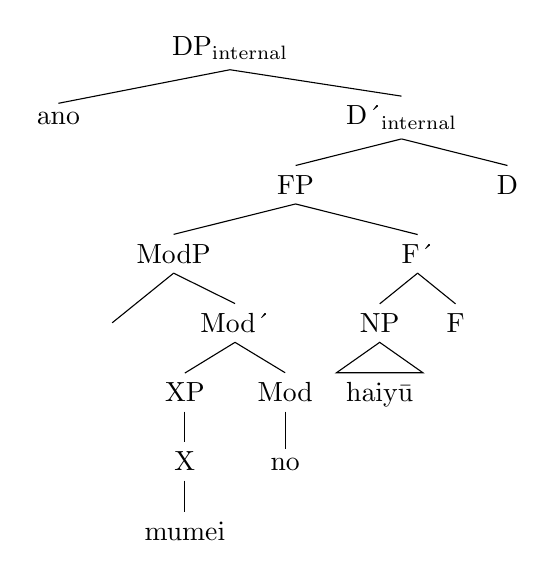
\begin{tikzpicture}[baseline=0pt, remember picture]
\tikzset{level distance=25pt, sibling distance=5pt}
 \Tree [.DP\textsubscript{internal} ano [.D´\textsubscript{internal} [.FP [.ModP {} [.Mod´ [.XP [.X mumei ] ] [.Mod no ] ] ] [.F´ [.NP \edge[roof]; haiyū ] F ] ] D ] ]
\end{tikzpicture}

Crucially, this account can be applied to all kinds of modifiers, lexical or functional, independent of word class and modification type. In all cases, \textsc{mod} selects the modifier and this chunk is situated in the Spec position of a functional projection within the relevant domain. Before outlining the concrete cases in Chapter \ref{modintegration}, I will discuss the precise semantics and contribution of this element, its application to the other modifiers, some refinements and some possible alternatives.

\subsection{More on the precise semantics and contribution of MOD} \label{semantics mod}

As mentioned in the preceding section, several linker architectures have been proposed and they mostly differ in the universality and precise contribution of the linker, as well as its semantics.\footnote{I am grateful to an anonymous reviewer for encouraging me to include this section.} For instance, \citet{philip:2012:linkers} in a study on a variety of typologically unrelated languages defines linkers as functional elements devoid of semantics that must intervene structurally to highlight modification. As she remarks ``[...] the linker does not initiate the relationship between Head and Dependent; it simply marks its presence." \citep[65]{philip:2012:linkers}. She includes Japanese in her sample and also concludes that \textsc{no} is such a linker. On the contrary, \citet{franco:2015:linkers} argue that linkers are not semantically vacuous, but have interpretive properties. However, the authors remain agnostic about the universality of linkers.

In the system defended here, \textsc{mod} is, in fact, demanded by the syntax in order for any element to function as a nominal modifier. It thus not only marks the relationship, it establishes the relationship. In Japanese, it is, furthermore, overtly realized in all instances of non-finite (that is: tenseless) modification. I furthermore argue that it is present, but unpronounced when it selects a finite modifier, i. e. a verbal relative clause. This means that in stances such as \ref{dearuno} above, it is not replaced or paraphrased by the copula, and the element /no/ is not an allomorph of it. Rather, since the modifier is predicative in nature, the copula can be overtly realized, which, in turn, causes the non-pronouncement of \textsc{mod}. See Chapter \ref{indirect mod} for more discussion.\footnote{Naturally, this begs the question why the forms /no/, or /na/ respecitively, and /de aru/ can alternate in attributive position. I argue that the latter is the optional realization of the copula. This accounts for the fact that this option is less natural. Simply realizing the syntactic head \textsc{mod} in absence of the copula is preferred.}

However, importantly, \textsc{mod} does not contribute semantics (in the strict sense) by itself and neither does it determine the type of a modifier or its contribution. In this point, I deviate from \citet{rubin:1994:mod}, who argues that \textsc{mod} necessarily contains a semantic component: Namely that of type-shifting lexemes from type ⟨e,t⟩ to type ⟨⟨e,t⟩,⟨e,t⟩⟩, thus from predicates to attributes (\citealt[171–177]{rubin:1994:mod} cf. \citealt{partee:1986:noun}). However, this poses immediate problems when considering quantificational modifiers and numerals. Those obligatorily co-occur with \textsc{no} in Japanese, but are not of the basic type ⟨e,t⟩, but ⟨⟨e,t⟩,t⟩ \citep{partee:1986:noun}, thus would not be the right input for \textsc{mod}.\footnote{This also extends to several non-intersective modifiers such as \textit{mere} or \textit{only}, which have \textit{per se} a quantifier-like character, and counterparts of which also only appear with \textsc{no} (see Chapter \ref{non-intersective Japanese}). I am grateful to David Adger for pointing out this latter point to me.}

This also clearly sets \textsc{mod} apart from the application of a similar syntactic head \textsc{join} proposed in \citet{truswell:2004:attributive, truswell:2009:attributive} and argued for in \citet{belk:2017:attributes}. Belk proposes a very similar account to \textsc{mod}, with the crucial difference that the lexical category of the input argument must be that of an adjective, which is of the basic type ⟨e,t⟩ \citep{partee:1986:noun}, and the output is always an attributive adjective \citep[ch. 2.3]{belk:2017:attributes}, where \textit{attributive} corresponds to \textit{direct} in \citet{cinque:2010:adj}. The upshot of this is that \textsc{join} immediately licenses attributive modification by adjectives without having to assume set intersection. It is therefore predominantly suitable for non-intersective adjectives \citep[37–38]{truswell:2004:attributive}. Adjectives which are licensed via \textsc{join} arguably come with this information in their lexicon \citep[157]{belk:2017:attributes}.

Rather, \textsc{mod} licenses modification, but the role of the modifier, whether it is direct or indirect, is determined in the syntax, This means that \textsc{mod} can select direct and indirect modifiers alike. In this sense, \textsc{pred} and \textsc{mod} are also not distributed alongside indirect and direct modification respectively, but \textsc{pred} is always present with (finite) predication, whereas \textsc{mod} is always present in modification structures, those of predicative modifiers alike.

\subsection{The application to \textit{i}- and \textit{na}-adjectives} \label{appl adj}

Here, I extend the analysis of \textsc{mod} as a universal head to the other monomoraic elements, \textsc{i} and \textsc{na}. All are realizations of the same element and the differences between these three elements is straightforwardly accounted for. Contrary to \textsc{no}, \textsc{i} and \textsc{na} are specified for the word classes they co-occur with, namely \textit{i}-adjectives and \textit{na}-adjectives respectively. This allows for the formulation of a spell-out rule for \textsc{mod} which makes use of word classes. %\is{Japanese adjectives}

\ex. Spell-Out Rule for \textsc{mod} in Japanese\\
$[Mod]$ $\leftrightarrow$ /i/ / iA \_ \\
\phantom{$[Mod]$ $\leftrightarrow$} /na/ / naA \_ \\
\phantom{$[Mod]$ $\leftrightarrow$} /no/ \label{spelloutrule}

This rule states that \textsc{mod} is realized as /i/ following \textit{i}-adjectives, as /na/ following \textit{na}-adjectives, and as /no/ after all other modifiers. That means that the spell-out forms /i/ and /na/ are more specified, and only occur after the word classes of \textit{i}- and \textit{na}-adjectives respectively, /no/ is underspecified, making it the elsewhere case. I assume that this rule is achieved via Late Insertion for functional elements \citep{halle:1993:distributed, chomsky:2001:derivation}, ensuring that the realization of \textsc{mod} can take place after it has entered syntax. Importantly, \textsc{mod} is a syntactic head that is only active within the DP, therefore the rule in \ref{spelloutrule} only refers to attributive contexts. The relevant structures for lexemes belonging to the two Japanese adjective groups in attributive position thus look as follows. %\is{Mod}

\newpage

\ex. \label{takaimod2} \ag. taka-i doresu\\
expensive-\textsc{mod} dress \\
`expensive dress’ \null \hfill (= \ref{takaimod1})
\b. 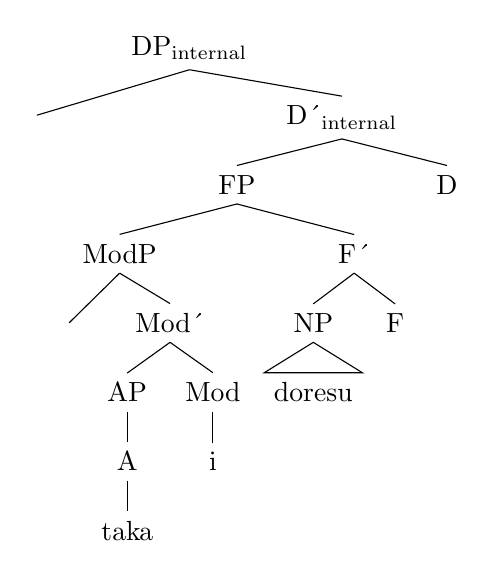
\begin{tikzpicture}[baseline=0pt, remember picture]
\tikzset{level distance=25pt, sibling distance=5pt}
 \Tree [.DP\textsubscript{internal} {} [.D´\textsubscript{internal} [.FP [.ModP {} [.Mod´ [.AP [.A taka ] ] [.Mod i ] ] ] [.F´ [.NP \edge[roof]; doresu ] F ] ] D ] ]
\end{tikzpicture}

\ex. \label{shikkunamod2} \ag. shikku-na doresu\\
chic-\textsc{mod} dress\\
`chic dress’ \null \hfill (= \ref{shikkunamod1})
\b. 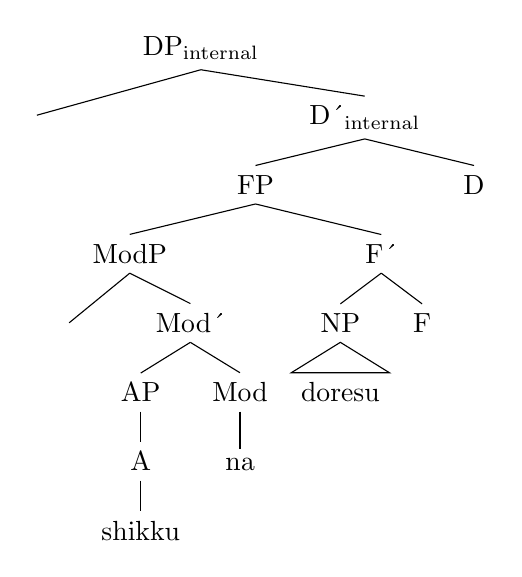
\begin{tikzpicture}[baseline=0pt, remember picture]
\tikzset{level distance=25pt, sibling distance=5pt}
 \Tree [.DP\textsubscript{internal} {} [.D´\textsubscript{internal} [.FP [.ModP {} [.Mod´ [.AP [.A shikku ] ] [.Mod na ] ] ] [.F´ [.NP \edge[roof]; doresu ] F ] ] D ] ]
\end{tikzpicture}

There are some potential caveats with this application worth mentioning. First, diachronic facts tell us that \textsc{no} is already attested in Old Japanese where it had the function of connecting two nouns (\citealt{frellesvig:2010:history} among others). From there, it only later entered other domains (\citealt{sakurai:1964:meiyo, wenck:1974:systematische}). On the other hand, \textsc{na} is derived from the historical copula \textit{nari} (attributive form \textit{naru}) and developed parallel to \textsc{da}, the short form of the copula confined to predicative position (\citealt{kubo:1992:japanese, urushibara:1993:syntactic, nishiyama:1999:adj, miyama:2011:da}). In the case of \textit{i}-adjectives, their inflectional paradigm differentiated between attributive -\textit{ki} and sentence-final -\textit{shi}, same as other verbal categories. Arguably, the morpheme \textsc{ki} is the predecessor of modern -\textsc{i} as a result of sound changes and diachronic omission of the velar /k/.\footnote{See for an analysis \citet[sec. 3.3]{nishiyama:1999:adj} and Chapter \ref{kitoi} of this book. For discussion on historical facts, see \citet{urushibara:1993:syntactic} and \citet{frellesvig:2010:history}.} This means that \textsc{no} could also at earlier stages of the language be identified as an individual morpheme, whereas the two other elements were parts of the inflectional system of Japanese adjectives. Researchers might therefore be hesitant to apply the Mod-hypothesis to the elements \textsc{i} and \textsc{na}.

Another potential problem is that the morpheme \textsc{i} does not only occur in attributive position, but also in predicative position.

\ex. \ag. taka-*(i) doresu\\
expensive-i dress\\
`expensive dress'
\bg. Ano doresu-wa taka-*(i).\\
that dress-\textsc{top} expensive-\textsc{i}\\
`That dress is expensive.'

Siince \textsc{mod} only occurs in attributive position, an alternative account needs to be posited for \textsc{i} in predicative position. In Chapter \ref{copulaelements}, I will put forth an analysis of \textsc{i} in predicative position as an instance of the copula \citep{nishiyama:1999:adj} and discuss why this analysis is not readily applicable to attributive \textsc{i}.

Nevertheless, as to be discussed further below, the account of all three elements as instances of \textsc{mod} makes the system adopted here consistent and avoids many of the problems of other accounts. Furthermore, it allows to reduce all three elements to the same underlying type, namely a functional head responsible for attributive modification.

\subsection{Restrictions}

As already visible in the examples above, the distribution of \textsc{mod} is not free. It is a dependent element and needs to select an element as attributive modifier. It attaches to this modifier and is confined in its realization to the overt realization of the modifier itself. It thus behaves as expected from functional elements (cf. \citealt[ch. 2.2.2]{rubin:1994:mod}). Furthermore, it needs to occur DP-internally, thus in the context of nominal modification. These two restrictions are intertwined and can be formulated in the refinement rule in \ref{refinementmod}. %\is{Mod}

\ex. Realization of \textsc{mod} in Japanese, refinement\\
1) \textsc{mod} must select a modifier which must be overtly realized. \\
2) \textsc{mod} only occurs within the DP. \label{refinementmod}

The requirement to select a modifier which must be overtly realized can be illustrated with instances of so-called \textit{light nouns}. In cases where English applies \textit{one}-substitution of nominal constituents \ref{redshirts}, Japanese also must employ a placeholder with a nominal character, called \textit{light noun} in \citet{hiraiwa:2012:mechanism}. Unfortunately, the most basic light noun is \textit{no}, thus homophonous to \textsc{mod}, as shown in the DP in \ref{redshirtsjapanese}. %\is{ellipsis}

\ex. I like red shirts, but I hate blue *(ones). \label{redshirts}

\exg. Aka-i shatsu-wa suki-da kedo, ao-i *(no)-wa kirai-da.\\
red-\textsc{mod} shirt-\textsc{top} like-\textsc{cop} but blue-\textsc{mod} \textsc{ln}-\textsc{top} hate-\textsc{cop}\\
`I like red shirts, but I hate blue ones.’ \label{redshirtsjapanese}

When a noun is pronominalized with the light noun \textit{no} `(the) one’, but modified by a \textit{no}-modifier, subsequent haplology causes one of the two elements to be deleted \citep[13531–1352]{hiraiwa:2016:ellipsis}. In \ref{haplology}, \textit{no} could be \textsc{mod} or the light noun. %\is{light noun}

\exg. Kuruma-wa Nihon no ga suki-da.\\
car-\textsc{top} Japan \textsc{mod}/\textsc{ln} \textsc{nom} be.fond-\textsc{cop}\\
`As for cars, I like Japanese ones.’ \label{haplology}

However, the point can be made clear by using other, more specified, light nouns such as \textit{mono} `thing’, which replaces the noun \textit{kuruma} `car’ in the second instance in \ref{watashino}. It is itself modified by a nominal possessor and this possessor must be licensed by \textsc{mod}, which is realized as /no/.

\exg. Kono kuruma-wa watashi-no mono desu.\\
this car-\textsc{top} I-\textsc{mod} \textsc{ln}.thing \textsc{cop.pol}\\
`This car is mine.’ \label{watashino}

Such examples thus show that \textsc{mod} must form a syntactic constituent with the modifier, hence neither of the two can be elided individually.

 \ref{refinementmod} also explains why \textsc{mod} does not appear outside of modificational contexts.\footnote{The fact that \textsc{mod} is not realized when the head of I is overt, will be discussed in Chapter \ref{indirect mod}.} This includes predicative contexts, but also accounts for clausal (floating) quantifiers mentioned in Chapter \ref{focus,japanese} and repeated below. Since the quantifier is part of the DP, thus is no modifier, \textsc{mod} is not realized.

\exg. Ni-satsu-dake, hon-wo kat-ta.\\
two-\textsc{cl}-only, book-\textsc{acc} buy-\textsc{acc}\\
`I bought only two books.’ (Lit. `Two only, I bought books.’) \null \hfill (= \ref{nisatsudake})

This restriction can be further illustrated via an example of a so-called \textit{major subject construction} \citep{kuroda:1992:japanese, heycock:1993:focus, vermeulen:2005:poss} given in \ref{joseigadoresuga} and elaborated in detail in Chapter \ref{majorsubject}. %\is{major subject construction}

\newpage

\exg. Sono josei-ga doresu-ga utsukushi-i.\\
this woman-\textsc{nom} dress-\textsc{nom} beautiful-\textsc{i}\\
`As for this woman, her dress (= the dress of this woman) is beautiful.’ \label{joseigadoresuga}

In \ref{joseigadoresuga}, the two nouns \textit{doresu} `dress’ and \textit{josei} ` woman’ stand in a possessor-possessee relationship. They both appear with the nominative case marker -\textsc{ga}, but while the lower noun is theta marked, the higher \textit{ga}-marked noun has a focus interpretation (see \citealt{heycock:1993:focus, vermeulen:2005:poss}). Importantly, the two nouns are not syntactically embedded in a modification structure and \textit{doresu} is devoid of an overt modifier. The underlying structure of \ref{joseigadoresuga} is arguably \ref{joseiunderlying} in which the possessor of the dress appears overtly \citep{kuroda:1992:japanese}. The entity \textit{josei} `woman’ appears twice making this sentence pragmatically marked. However, crucially, as it fulfills the role of a modifier of \textit{doresu} `dress’, it is obligatorily followed by \textsc{no}, contrary to \ref{joseigadoresuga}.

\exg. Sono josei-ga (sono) josei-no doresu-ga utsukushi-i.\\
this woman-\textsc{nom} this woman-\textsc{mod} dress-\textsc{nom} beautiful-i\\
`As for this woman, the dress of this woman is beautiful.’ \label{joseiunderlying}

The crucial part is that to arrive from \ref{joseiunderlying} at \ref{joseigadoresuga}, not only the nominal part \textit{(sono) josei} `(this) woman’ is deleted, but also \textsc{no}. There is no modifier to select, hence \textsc{mod} is not present in the structure and not realized.

\subsection{Discussion: Alternative accounts} \label{comparisonpreviousno}

In this section, I will quickly compare the idea presented here to alternative accounts and show why it fares better.

\subsubsection{Post-syntactic insertion}

\textsc{mod} as depicted here is very similar to the well-known \textit{Mod-Insertion Rule} of \citet{kitagawa:1982:prenominal}, and see \citet{watanabe:2010:notes}, which became a landmark proposal for authors arguing for a single syntactic status of \textsc{no}. The revised version of this rule from \citet{watanabe:2010:notes} is given below.

\ex. Mod Insertion Rule (Revised): [DP . . . XP(–tense) N] \\ $\rightarrow$ [DP . . . XP(–tense) Mod N], where head noun is overt and Mod $=$ \textit{no} \\ \null \hfill \citep[66]{watanabe:2010:notes}

Essentially, this rule states that the element \textsc{no} is inserted post-syntactically whenever modification happens. However, it is subsequently deleted when the modifying element contains tense, which explains why it never co-occurs with relative clauses. By including this aspect, the authors point out a crucial difference between Japanese and Mandarin, where \textsc{de} does obligatorily follow relative clauses.

In a nutshell, in the account defended here, \textsc{mod} is a functional category that is already present in the syntax and licenses lexical and functional elements as modifiers, whereas in the post-syntactic account of \citet{kitagawa:1982:prenominal}, \textsc{mod} gets inserted later after the relationship between modifier and noun has already been established. Both options are appealing, and there is no reason why the proposal of \citet{kitagawa:1982:prenominal} should be incompatible with the system defended here, which also relies on some form of Late Insertion \citep{halle:1993:distributed, chomsky:2001:derivation}, although to ensure the correct realization of \textsc{mod}.

I argue that the analysis of \textsc{no} as a syntactic head is preferable from a theoretic perspective, as it fits better with the cartographic framework adopted here. Furthermore, it has the big advantage of being more language-universal, allowing to explain phenomena in a variety of different languages with regard to such syntactic heads involved in modification, contrary to the highly language-specific Mod Insertion rule.

One concrete argument against post-syntactic analyses of linkers, also provided in \citet[54–55]{philip:2012:linkers}, is that, as for instance shown in the examples \ref{watashino} and following, is that \textsc{mod} forms a syntactic constituent with the modifier, evidenced by the fact that neither can be elided without the other. If \textsc{mod} was post-syntactically inserted, it would be odd if neither, the modifier itself or the linker, could survive elision of the other element.

\subsubsection{Pre-syntactic insertion}

An analysis that is worth considering, but ultimately not suitable is pre-syntactic insertion, for instance along the lines of a \textit{word marker} hypothesis proposed prominently in \citet{alex:2008:class} for the inflectional endings of nouns in German, Russian and Greek, following several predecessors \citep{harris:1991:exponence, ritter:1993:where, aronoff:1996:morphology, oltra:1999:on, oltra:2005:stress} . Word markers are pre-syntactically inserted elements, that are bestowed with a variety of binary features and these features match those of the different inflectional classes and cases of nouns in these languages \citep[33]{alex:2008:class}. One could entertain the idea that \textsc{no} is a word marker that is pre-syntactically added to lexical and functional elements to form a compound structure. The obvious problem is that we would never expect this word marker to be absent once the lexical element has entered syntax (Artemis Alexiadou p.c.). Recall however that \textsc{no} never appears in predicative position. %\is{word markers}

\exg. Ano haiyū-wa mumei- (*no) da.\\
that actor-\textsc{top} unknown \textsc{no} \textsc{cop}\\
`That actor is unknown.’ \\ \null \hfill (= \ref{nopredicativeno})

If \textsc{no} was a word marker, it should be able to appear in predicative contexts, but this is illicit. Furthermore, we would never expect such a marker to be attracted to functional elements, such as postpositions. However, \textsc{no} can follow postpositions in modificational contexts, as alluded to in the introductory chapter.

\exg. ishi-de-no kōgeki\\
stone-\textsc{ins-no} attack\\
`an attack with stones' \null \hfill \citep[248]{saito:2008:N}

\subsubsection{Lexical compounds}

One might also entertain the possibility that two adjacent elements, especially nouns, out of which the first one is followed by \textsc{no}, actually do not mark cases of modification, but of lexical compound formation. A crucial fact which shows that the construction at hand is not an instance of compound formation is that the first noun can be anaphorically bound as shown in \ref{senseinohon}, which offers an ambiguous interpretation: The internal argument of the matrix verb has been dropped and either ones of the nouns in the subordinate clause, the head noun or its modifier, could serve as the antecedent, as indicated via the indices.

\exg. Sensei\textsubscript{1}-no hon\textsubscript{2}-wo yon-de, \textit{pro}\textsubscript{1/2} suki-ni nat-ta.\\
teacher-\textsc{mod} book-\textsc{acc} read-\textsc{ger} pro be.fond-\textsc{dat} become-\textsc{pst}\\
1. $\approx$ `Having read the teacher’s\textsubscript{1} book\textsubscript{j}, \textit{pro} became fond of it\textsubscript{2}.’\\
2. $\approx$ `Having read the teacher’s\textsubscript{1} book\textsubscript{j}, \textit{pro} became fond of him/her\textsubscript{2}.’ \label{senseinohon}

This shows that the modifier \textit{sensei-no} `teacher’s’ must have a syntactic status, and is not part of a compound. Compare this to the ungrammatical English example containing a lexical compound below. Here, the first part of the compound cannot serve as an antecedent to the pronoun \textit{it}.

\ex. *With my sun\textsubscript{1} glasses, I am protected from it\textsubscript{1} well. \\ \null \hfill \citep[37]{rae:2010:ordering}

\subsubsection{Only predication and only attribution}

Obviously, analyses that derive \textsc{no} from a predicate structure are not tenable, given the many direct \textit{no}-modifiers mentioned thus far and attested in the data set. \citet{dikken:2004:complex}, cf. \citet{dikken:2006:relators, moro:1997:raising}, treat \textsc{no} parallel to English DPs with the element \textit{of} as shown below together with the underlying structure. %\is{predicate inversion}

%\newpage

\ex. \a. a jewel of a village \hfill \citep[162]{dikken:2006:relators}
\b. [\textsc{rp} [village][\textsc{relator} [\textsc{similar} jewel]]] \hfill \citep[178]{dikken:2006:relators}

The underlying structure contains the predicate \textsc{similar} whose head is empty and which needs to be licensed. This licensing is achieved via predicate inversion. Concretely, the predicate complement moves to the Spec position of the \textsc{relator} which is spelled out in English as /of/ \citep[ch. 5]{dikken:2006:relators}. The reason for this is to achieve a different (contrastive) information structure. In addition to the problem that the different head-parameter of Japanese leads to problems in word order, this proposal is not tenable as it predicts all \textit{no}-modifiers to be indirect.\footnote{The same holds for \citet{koopman:2016:further}, who propose a relative clause account for \textit{no}-modifiers.}

On the other hand, one could be tempted to reduce \textsc{mod} only to structures in which direct modification is at stake. I discussed this point already in Chapter \ref{semantics mod}, where I gave a reference to \citet{belk:2017:attributes}, who argues that \textsc{join} (our \textsc{mod}) selects adjectives and produces attributive adjectives, that is direct adjectives \citep[ch. 2.3]{belk:2017:attributes}. However, this account crucially undergenerates, since \textsc{no} also co-occurs with indirect modifiers, nominal lexemes (\textit{Nihon-no} `Japan(-ese)’) and also functional elements (\textit{doko-no} `where’).

\subsubsection{Alternatives for I and NA}

Some other noteworthy analyses for \textsc{i} and \textsc{na} were mentioned in Chapter \ref{intro japanese}. The prominent analysis to be adopted for the former element, and the counterpart to \textsc{na} in \textit{predicative} position is that of a combination as copula and tense element (Chapter \ref{copulaelements}), but for the reasons mentioned above (direct modification and \textsc{mod} being restricted to DP-internal environments), this account does not extend to the attributive occurrence of these elements. A noteworthy alternative is the case marker hypothesis defended in \citet{yamakido:2005:nature} and \citet{larson:2008:ezafe}, according to which \textsc{i} and \textsc{na} receive an analysis identical to the \textit{ezāfe} morpheme in Western Iranian languages as case markers. The authors also propose an account that reduces the different output to the different word classes, but handle it via resorting to case. This analysis suffers from the problem that it does not become clear why \textsc{i} and \textsc{na} are always present, even in relative clause structures, thus in larger structures where it is not clear how case is assigned. %\is{ezāfe}

\newpage

\exg. kami-ga kirei-na hito\\
hair-\textsc{nom} pretty-\textsc{na} person\\
`a person whose hair is pretty' \null \hfill \citep[34]{kaplan:1995:the}

The analysis of \citet{yamakido:2005:nature, larson:2008:ezafe} does not foresee the option of the case marker to occur with CPs (or even IPs) as also criticized for instance by \citet{samvelian:2008:ezafe, kahne:2014:revisiting} for the Persian data. It furthermore remains unclear why the respective elements should disappear, for example when modifiers inflect for past. As \citet[Fn. 25, p. 296]{watanabe:2013:non} notes, ``This proposal is untenable for the reason that the sensitivity to tense is left unexplained.’’

\subsection{Application: Integration via \textsc{Mod}} \label{modintegration}

Above, I defended the \textsc{mod}-hypothesis and explained why it fares better than most alternatives. In the following subsections, I will discuss how each modifier that is selected via \textsc{mod} is embedded in the DP in line with the cartographic research program. As discussed, for instance in Chapter \ref{semantics mod}, \textsc{mod} does not differentiate between modification type, word class or other factors.

\subsubsection{Structure for direct modifiers}

Exemplified with the non-intersective \textit{no}-modifier \textit{shōrai-no} `future’ discussed above, the structure of a direct modifier within the DP is as follows.\footnote{Recall that demonstratives such as \textit{ano} `that’ are specifiers in Japanese, accounting for the correct word order.} %\is{direct modifiers}

\ex. \label{shoraimod} \ag. ano shōrai-no purosakkāsenshu\\
that future-\textsc{mod} pro.soccer.player\\
`that future professional soccer player’
\b. 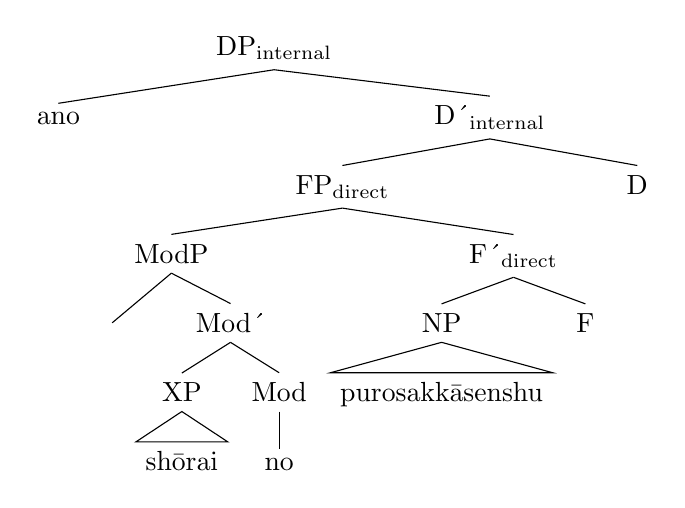
\begin{tikzpicture}[baseline=0pt, remember picture]
\tikzset{level distance=25pt, sibling distance=5pt}
 \Tree [.DP\textsubscript{internal} ano [.D´\textsubscript{internal} [.FP\textsubscript{direct} [.ModP {} [.Mod´ [.XP \edge[roof]; shōrai ] [.Mod no ] ] ] [.F´\textsubscript{direct} [.NP \edge[roof]; {purosakkāsenshu} ] F ] ] D ]]
\end{tikzpicture}

The relevant assumptions are simple: Since the modifier \textit{shōrai-no} `future’ is direct, it is merged in the direct domain in an unspecific functional projection. It is selected by \textsc{mod} and licensed as an attributive modifier. As the word class status of \textit{shōrai-no} is unclear, I adopt the label XP. The head of \textsc{mod} is spelled out as /no/. This is the structure to be adopted for all direct modifiers.

\subsubsection{Structures for indirect modifiers} \label{indirect mod}

More must be said about indirect modifiers. Recall that as long as a modifier can principally appear in predicative position it is ambiguous between a direct and an indirect status. This is, for example, the case for \textit{mumei-no} `unknown’ repeated from \ref{anomumei} and given alongside the relevant predicative occurrence. %\is{indirect modifiers}

\ex. \ag. ano mumei-no haiyū\\
that unknown-\textsc{mod} actor\\
`that unknown actor’
\bg. Ano haiyū-wa mumei-da.\\
that actor-\textsc{top} unknown-\textsc{cop}\\
`That actor is unknown.’

 Indirect modifiers are embedded along the lines in \ref{mumeicp} exemplified with \textit{mumei-no} in a status as indirect modifier.

\ex. \label{mumeicp} 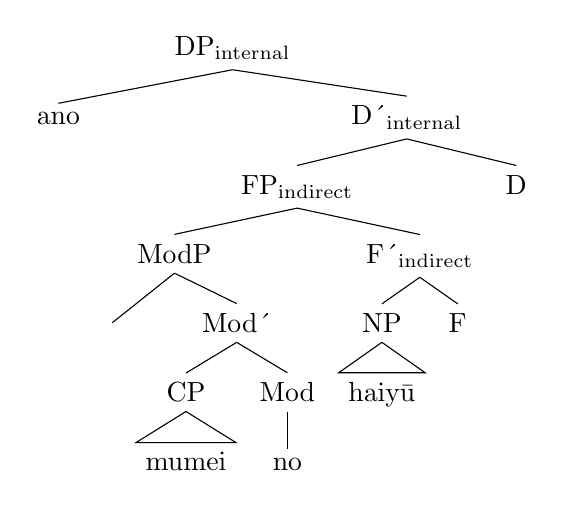
\begin{tikzpicture}[baseline=0pt, remember picture]
\tikzset{level distance=25pt, sibling distance=5pt}
 \Tree [.DP\textsubscript{internal} ano [.D´\textsubscript{internal} [.FP\textsubscript{indirect} [.ModP {} [.Mod´ [.CP \edge[roof]; mumei ] [.Mod no ] ] ] [.F´\textsubscript{indirect} [.NP \edge[roof]; haiyū ] F ] ] D ]]
\end{tikzpicture}

Indirect modifiers are merged in the specifier position of functional projections inside the indirect domain. Like \textit{shōrai-no} `future’ in \ref{shoraimod}, indirect modifiers are licensed via \textsc{mod} in attributive position. Depending on the word class of the preceding modifier, \textsc{mod} is spelled out as /i/, /na/ or /no/. In this case, it licenses the \textit{no}-modifier \textit{mumei-no} and is realized as /no/.

A crucial difference between indirect and direct modifiers, besides the different positions inside the DP, is that indirect modifiers are embedded in larger structures. As outlined earlier in this chapter and motivated in Chapter \ref{cinque adj}, I assume indirect modifiers to be CPs.

Crucially, however, it is not the case that in all CPs, an instance of \textsc{mod} overtly appears. Recall that \textsc{no} never follows verbal relative clauses in Japanese, and neither do \textsc{i} or \textsc{na}, contrary to Mandarin \textsc{de}, as illustrated once more below.

\exg. [\textsubscript{CP} kare-ga kat-ta] (*no) hon\\
{} he-\textsc{nom} buy-\textsc{pst} \textsc{no} book\\
`the book that he bought’

The relevant elements are neither present when adjectives are inflected for past, or when the canonical forms of the copula, \textsc{de-ar-u} for non-past and \textsc{d(e)-at-ta} for past appear.

%\newpage

\ex. \ag. ano taka-katta (*i) doresu\\
that expensive-\textsc{pst} \textsc{i} dress\\
`that dress which was expensive' \null \hfill \textit{i}-adjective, past
\bg. ano shikku-dearu (*na) doresu\\
that chic-\textsc{cop} \textsc{na} dress\\
`that dress which is chic’ \null \hfill \textit{na}-adjective, non-past
\cg. ano mumei-dearu (*no) haiyū\\
that unknown-\textsc{cop} \textsc{no} actor\\
`that actor who is unknown' \null \hfill \textit{no}-modifier, non-past

Foreshadowing the analysis, what is crucial in these instances, is that overt tense appears.

Compare this to structures where, on the other hand, lexemes from the two adjective groups or the group of \textit{no}-modifiers co-occur with \textsc{mod}, but clearly have a clausal status. Prototypically, this happens when they co-occur with a subject. This is illustrated below for each word class.

\ex. \ag. Tarō-ga shujinkō-no monogatari\\
Taro-\textsc{nom} main.protagonist-\textsc{no} story\\
`story in which Taro is the main protagonist' \\ \null \hfill \textit{no}-modifier \citep[66]{watanabe:2010:notes}
\bg. kami-ga naga-i hito\\
hair-\textsc{nom} long-\textsc{i} person\\
`person whose hair is long' \\ \null \hfill \textit{i}-adjective \citep[1278]{miyagawa:2011:genitive}
\cg. shūshoku-ga taihen-na butsurigaku\\
job-\textsc{nom} hard-\textsc{na} physics\\
`physics, where finding a job is difficult' \\ \null \hfill \textit{na}-adjective \citep[255]{kuno:1973:structure}

Deterring a precise analysis of such constructions to Chapter \ref{majorsubject}, crucially, the modifiers in these examples are embedded into a CP, not just in a small clause or under PredP \citep{bowers:1993:predication}. First, there must at least be an IP-layer present to host the overt subjects alongside nominative case. In the examples above, this position, namely Spec, IP, is occupied by \textit{Tarō}, \textit{kami} `hair’ and \textit{shūshoku} `job’ respectively.

Furthermore, there is evidence that overt tense is implied in those examples, and this tense is non-past. Including a temporal adverb with reference to the present, such as \textit{genzai} `(at) present’, is unproblematic. Inserting, however, a temporal adverb denoting past, such as \textit{kakoni} `in the past’, leads to ungrammaticality. This shows that overt tense, temporal reference to the present, is contained in those modifiers, even when they co-occur just with the monomoraic elements. Observe the minimal pair in \ref{genzaikakoni}.

%\newpage

\ex. \label{genzaikakoni} \ag. Tarō-to Hanako-ga genzai shujinkō-no monogatari\\
Taro-\textsc{com} Hanako-\textsc{nom} at.present main.protagonist-\textsc{mod} story\\
`story in which Taro and Hanako are the main protagonists at present’
 \bg. *Tarō-to Hanako-ga kakoni shujinkō-no monogatari\\
Taro-\textsc{com} Hanako-\textsc{nom} in.the.past main.protagonist-\textsc{mod} story\\
(`story in which Taro and Hanako were the main protagonists in the past’)

These arguments show that those modifiers are at least of size IP, however, no overt tense morpheme is realized, i.e. the head of IP seems to be empty. In this study, I do treat all Japanese relative clauses as involving a CP-layer (for arguments see Chapter \ref{size,indirect}), therefore, the relevant structure is as in \ref{cps}, in which \textit{Tarō-ga shujinkō} is a CP which is selected by \textsc{mod} and licensed as attributive modifier. %\is{indirect modifiers}

\exg. [\textsubscript{DP} [\textsubscript{CP} Tarō-ga shujinkō-no] monogatari]\\
{} {} Taro-\textsc{nom} main.protagonist-\textsc{mod} story\\
`story in which Taro is the main protagonist' \null \hfill \citep[66]{watanabe:2010:notes} \label{cps}

Adopting an analysis along the lines of operator-derivation for relative clauses (Chapter \ref{operator}), the whole derivation embedded in the DP looks as follows. %\is{operator}

\newpage

\ex. \label{shujinkonostructure} \ag. Tarō-ga shujinkō-no monogatari\\
Taro-\textsc{nom} main.protagonist-\textsc{mod} story (= \ref{cps})\\
\b. \hspace{-3.5cm} 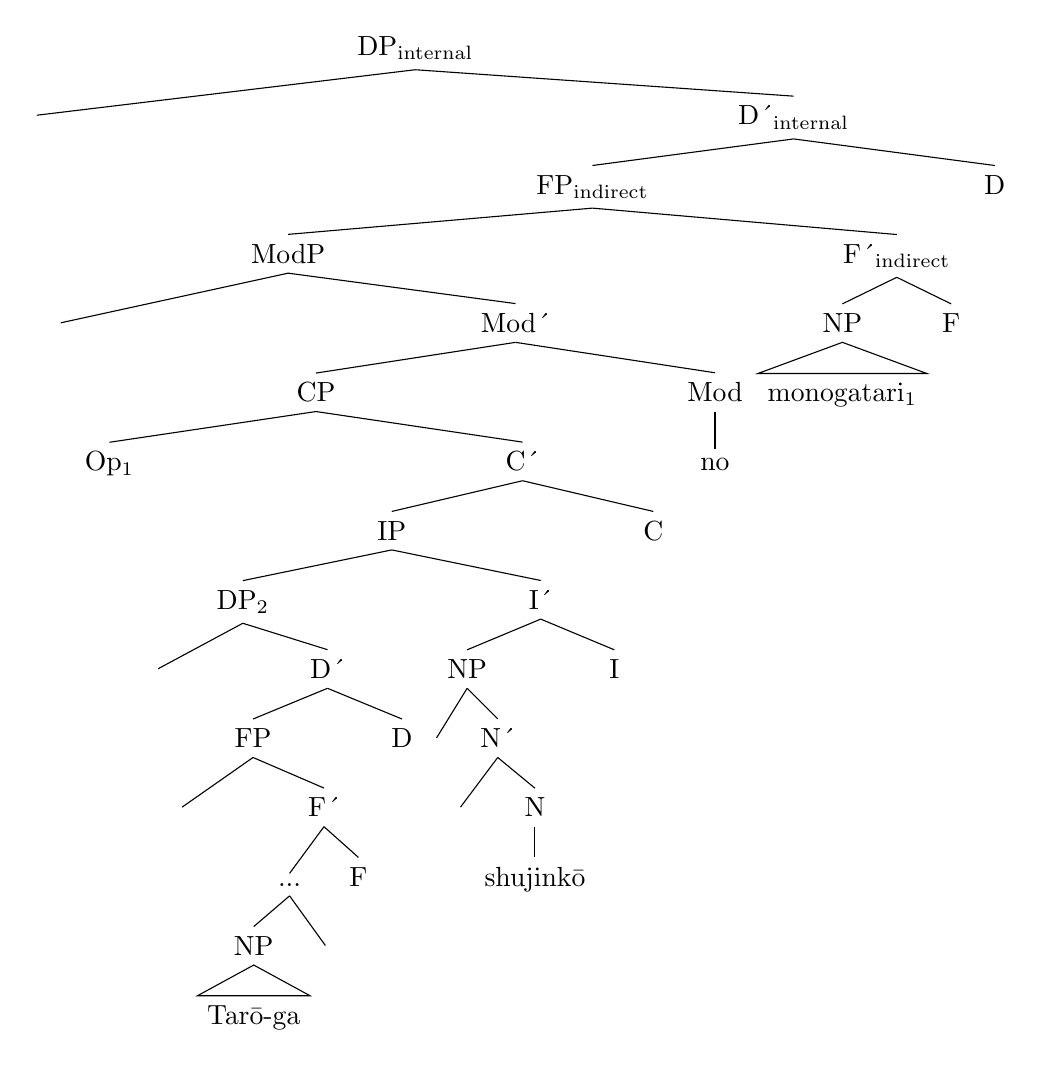
\begin{tikzpicture}[baseline=0pt, remember picture]
\tikzset{level distance=25pt, sibling distance=2pt}
 \Tree [.DP\textsubscript{internal} {} [.D´\textsubscript{internal} [.FP\textsubscript{indirect} [.ModP {} [.Mod´ [.CP Op\textsubscript{1} [.C´ [.IP [.DP\textsubscript{2} {} [.D´ [.FP {} [.F´ [.... [.NP \edge[roof]; Tarō-ga ] {} ] F ] ] D ] ] [.I´ [.NP {} [.N´ {} [.N shujinkō ] ] ] I ] ] C ] ] [.Mod no ] ] ] [.F´\textsubscript{indirect} [.NP \edge[roof]; monogatari\textsubscript{1} ] F ] ] D ]]
\end{tikzpicture}

The clausal modifier is embedded in a functional projection for indirect modifiers in the DP-internal domain. It is of size CP and selected by ModP whose head is spelled out as /no/ since the lexical head of the relative clause is a noun. The subject DP \textit{Tarō} is situated in Spec, IP where it receives nominative case. Embedded in the relative clause is an operator \textit{Op}, which moves to Spec, CP and is co-indexed with the noun \textit{monogatari} `story’, thereby ensuring that this noun is correctly interpreted inside the relative clause, solving the Connectivity Problem \citep{salzmann:2017:reconstruction}.

The question is where the operator exactly originates. There is reason to believe that it starts in the extended projection of the modifying NP (or more precisely DP, see below) \textit{shujinkō}. First, note that some relationship between \textit{monogatari} `story’ and \textit{shujinkō} `main protagonist’, one akin to possession, has to be established at some point in the derivation. This underlying relationship is given below for concreteness.\footnote{Note that the demonstrative \textit{sono} is in the specifier of the DP with the head noun \textit{shujinkō} and does not form a constituent with \textit{monogatari}.}

\ex. \ag. sono monogatari-no shujinkō\\
that story-\textsc{mod} main.protagonist\\
`the main protagonist of that story’
\b. 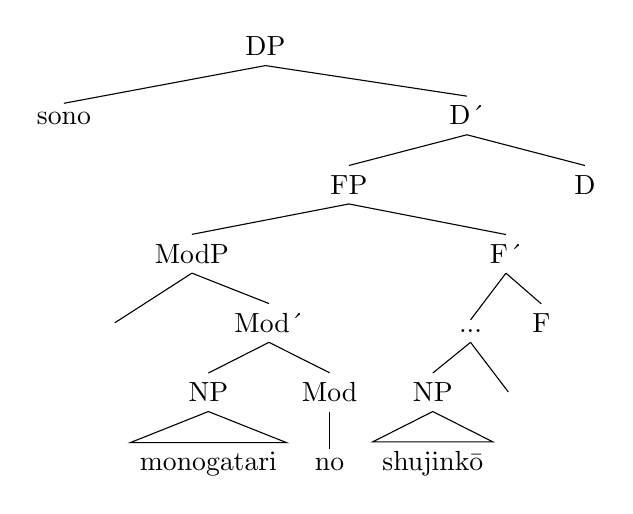
\begin{tikzpicture}[baseline=0pt, remember picture]
\tikzset{level distance=25pt, sibling distance=2pt}
 \Tree [.DP sono [.D´ [.FP [.ModP {} [.Mod´ [.NP \edge[roof]; monogatari ] [.Mod no ] ] ] [.F´ [.... [.NP \edge[roof]; shujinkō ] {} ] F ] ] D ] ]
\end{tikzpicture}

This means that the operator is a placeholder for \textit{(sono) monogatari} `(this) story’, as shown in \ref{placeholder}. %\is{operator}

\exg. [\textsubscript{DP} [\textsubscript{CP} Tarō-ga \textit{Op}\textsubscript{1} shujinkō-no] monogatari\textsubscript{1}]\\
{} {} Taro-\textsc{nom} Op main.protagonist-\textsc{mod} story\\
`story in which Taro is the main protagonist (of the story)’ \label{placeholder}

This gives good evidence that the operator starts out from deep within the relative clause, namely from a position in the extended projection of the modifying noun, which then actually constitutes a DP.

\ex. 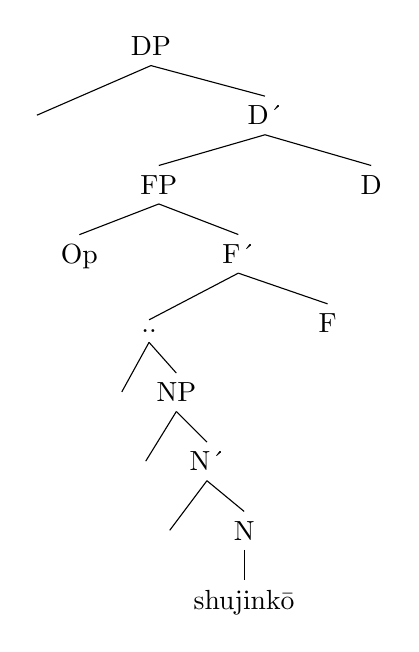
\begin{tikzpicture}[baseline=0pt, remember picture]
\tikzset{level distance=25pt, sibling distance=2pt}
 \Tree [.DP {} [.D´ [.FP Op [.F´ [... {} [.NP {} [.N´ {} [.N shujinkō ] ] ] ] F ] ] D ] ]
\end{tikzpicture}

From this deep position within the modifying DP, the operator moves to Spec, CP of the relative clause and ensures correct interpretation of the head noun and the relative clause as a whole. Crucially, again, within the relative clause a second concrete spell-out of \textsc{mod} is absent, as no overt modifier appears.

A remaining point left explained is why no instance of \textsc{mod} appears once the head of I is filled, i.e. once the inflectional forms \textsc{katta}, \textsc{dearu} or \textsc{deatta} are realized. The relevant structure of only the CP looks as follows.

\ex. \ag. [Tarō-ga shujinkō-de-at-ta] (*no) monogatari\\
Taro-\textsc{nom} main.protagonist-\textsc{pred-cop-pst} \textsc{mod} story\\
`story in which Taro was the main protagonist' \\ \null \hfill \citep[66]{watanabe:2010:notes} \label{shujinkodeatta}
\b. 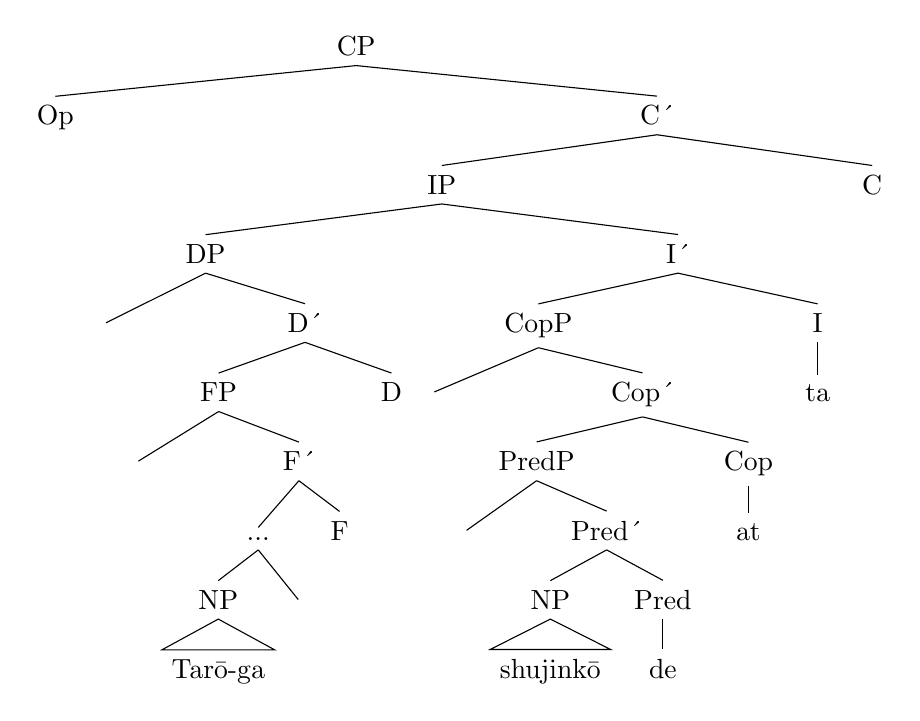
\begin{tikzpicture}[baseline=0pt, remember picture]
\tikzset{level distance=25pt, sibling distance=5pt}
 \Tree [.CP Op [.C´ [.IP [.DP {} [.D´ [.FP {} [.F´ [.... [.NP \edge[roof]; {Tarō-ga} ] {} ] F ] ] D ] ] [.I´ [.CopP {} [.Cop´ [.PredP {} [.Pred´ [.NP \edge[roof]; {shujinkō} ] [.Pred de ] ] ] [.Cop at ] ] ] [.I ta ] ]] C ] ]
\end{tikzpicture}

Embedded in the CP are the predicative copula \textsc{pred}, which is there to license predication and is realized as /de/ \citep{bowers:1993:predication, nishiyama:1999:adj}, alongside the dummy copula \textsc{cop} which offers be-support \citep{doron:1983:verbless, rapoport:1987:copular}, realized as /ar/. Furthermore, the head of I is overtly realized via the past morpheme -\textsc{ta}.\footnote{See Chapter \ref{copulaelements} for justification of these heads. From now on, I will adopt the respective glosses \textsc{pred} (predicative copula), \textsc{cop} (dummy copula) and \textsc{prs} or \textsc{pst} respectively for the tense morpheme, when the elements \textsc{de-ar-u}, \textsc{d(e)-at-ta} and \textsc{k-at-ta} occur.}

Again, overt tense, in this case past tense, is expressed. This can be evidenced via the impossibility to include a temporal adverb referring to the present, but the possibility of including a temporal adverb referring to past. Compare the minimal pair in \ref{kakonigeht} to the one in \ref{genzaikakoni} above.

\newpage

\ex. \label{kakonigeht} \ag. *[\textsubscript{DP} [\textsubscript{CP} Tarō-to Hanako-ga genzai shujinkō-de-at-ta] monogatari]\\
{} {} Taro-\textsc{com} Hanako-\textsc{nom} at.present main.protagonist-\textsc{pred-cop-pst} story\\
(`story in which Taro and Hanako are the main protagonists at present’)
 \bg. [\textsubscript{DP} [\textsubscript{CP} Tarō-to Hanako-ga kakoni shujinkō-de-at-ta] monogatari]\\
{} {} Taro-\textsc{com} Hanako-\textsc{nom} in.the.past main.protagonist-\textsc{pred-cop-pst} story\\
`story in which Taro and Hanako were the main protagonists in the past’

On a descriptive level, the overt realization of tense correlates with the absence of the overt realization of \textsc{mod}. This syntactic head is not realized when tense is overtly expressed. Thus, the question arises whether \textsc{mod} is still present in such circumstances, but somehow blocked from being realized, or whether CPs with an overt tense head are not licensed via \textsc{mod} in the first place.

Although, at the present moment, there is no concrete evidence for either of the two options, I have already mentioned at the beginning of this subsection that I will keep the analysis of \textsc{mod} as a universal syntactic head as consistent as possible. That means, I assume that it is always present structurally. However, it remains silent once the head of I is filled, i. e. once a finite indirect modifier occurs, where finiteness corresponds to the presence of tense and/or agreement (see \citealt[103–108]{landau:2013:control} for an overview as well as \citealt{nikolaeva:2007:intro} and articles cited therein). I leave it to future research to determine at which point its overt output gets deleted, or if it does not get realized in the first place. \footnote{This point extends to the realization of \textsc{mod} in other languages. See the discussion at the end of this chapter.}

The whole DP corresponding to \ref{shujinkodeatta} looks as follows. Take note that the subject position and derivation of the operator remain the same.\footnote{There are some noteworthy alternatives, which are also not entirely promising. If we assume a different CP-structure for examples such as \ref{cps}, it is unclear what this different CP should look like. If we argue that \textsc{mod} only selects those CPs which do not select PredP (and/or CopP), then why are verbal relative clauses not followed by \textsc{no}?

\par

Evidence from acquisition is also conflicting. \citet[chapters 4 and 5]{murasugi:1991:noun} shows that some Japanese children in her study overgenerated \textsc{no} and also used it after verbal relative clauses, a position not allowed in Standard Japanese. Some even produced it after adjectives either in addition to or instead of \textsc{i} and \textsc{na}. This could be taken as evidence that for those children \textsc{mod} is always present, but they have not learned the rules when to omit it. On the other hand, these results could also be interpreted in a way that the children did not know which CP they are producing and whether they need \textsc{mod} or not. See also \citet[ch. 3.5]{yamakido:2005:nature}.}

\newpage

\ex. \label{shujinkodatta} \ag. [Tarō-ga shujinkō-de-at-ta] monogatari\\
Taro-\textsc{nom} main.protagonist-\textsc{pred-cop-pst} story (= \ref{shujinkodeatta})\\
\b. \hspace{-2cm} 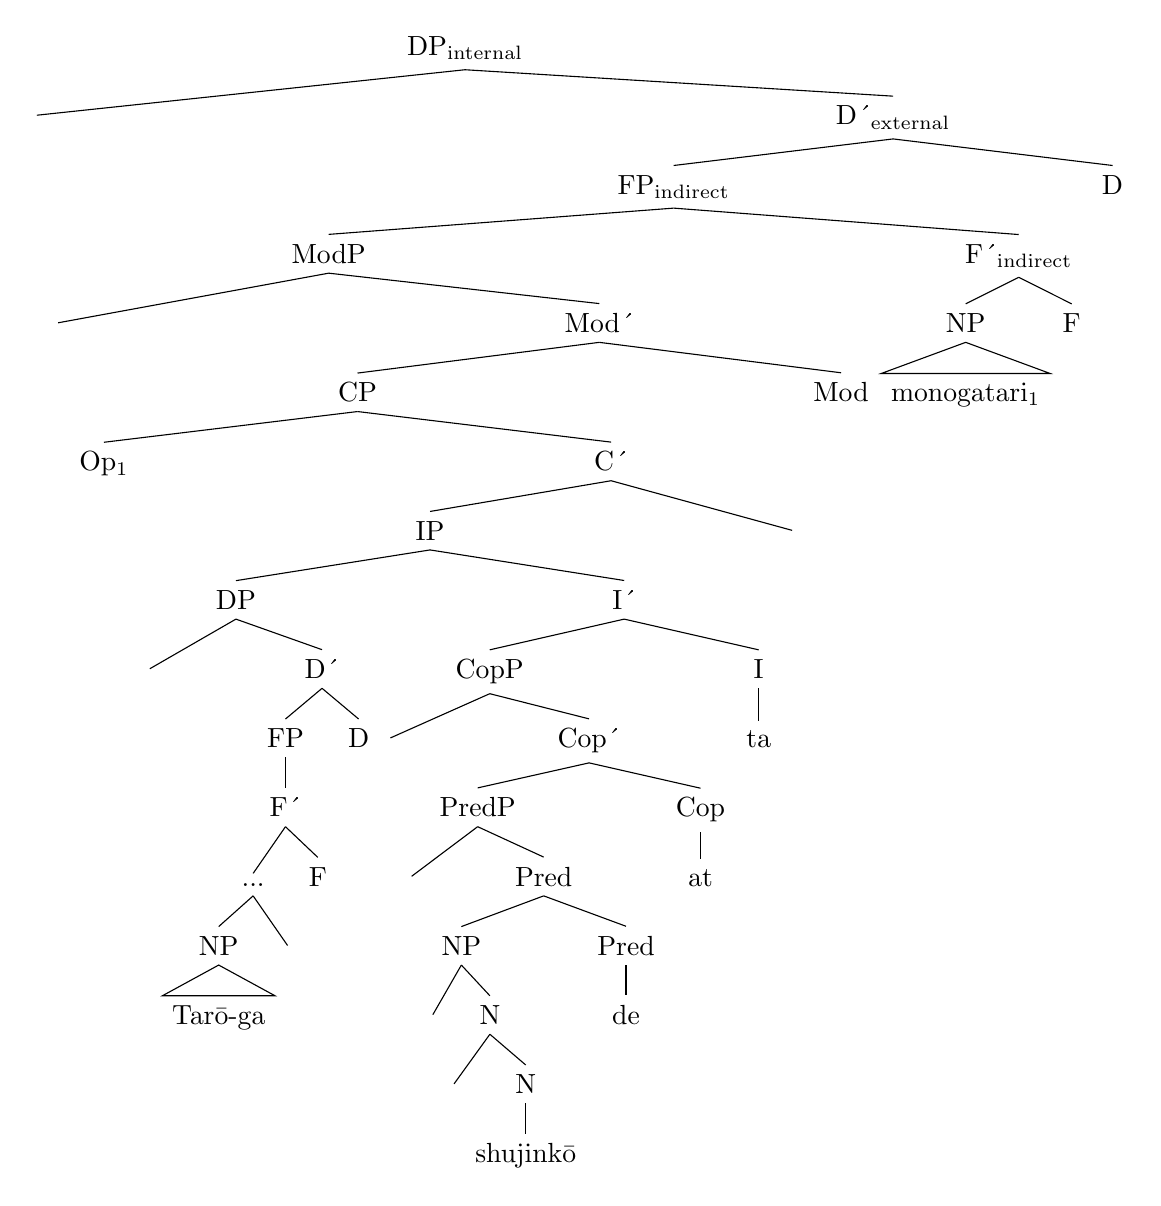
\begin{tikzpicture}[baseline=0pt, remember picture]
\tikzset{level distance=25pt, sibling distance=1pt}
\Tree [.DP\textsubscript{internal} {} [.D´\textsubscript{external} [.FP\textsubscript{indirect} [.ModP {} [.Mod´ [.CP Op\textsubscript{1} [.C´ [.IP [.DP {} [.D´ [.FP [.F´ [.... [.NP \edge[roof]; Tarō-ga ] {} ] F ] ] D ] ] [.I´ [.CopP {} [.Cop´ [.PredP {} [.Pred [.NP {} [.N {} [.N shujinkō ] ] ] [.Pred de ] ] ] [.Cop at ] ] ] [.I ta ] ] ] {} ] ] Mod ] ] [.F´\textsubscript{indirect} [.NP \edge[roof]; monogatari\textsubscript{1} ] F ] ] D ] ]
\end{tikzpicture}

To summarize, potentially all CPs are licensed via \textsc{mod} in attributive position, but \textsc{mod} is only realized when the head of IP remains empty.

\subsubsection{Structures for remaining modifiers} \label{other mod}

The structure for all other modifiers, including numerals and arguments, which also unequivocally appear with \textsc{no}, can, again, be derived in a straightforward manner. All these modifiers are embedded in the relevant functional projection and selected by \textsc{mod}, whose head is spelled out as /no/. Their syntactic role is determined in the syntax. %\is{numeral}

\newpage

\ex. A \textsc{mod}-structure for numerals
\ag. futari-no gakusei\\
two-\textsc{mod} student\\
`two students’
\b. 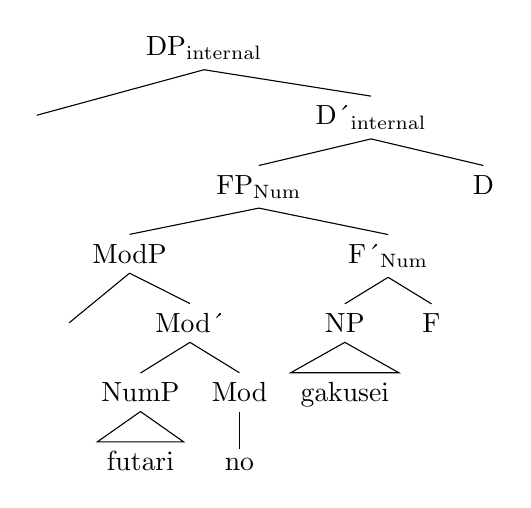
\begin{tikzpicture}[baseline=0pt, remember picture]
\tikzset{level distance=25pt, sibling distance=5pt}
 \Tree [.DP\textsubscript{internal} {} [.D´\textsubscript{internal} [.FP\textsubscript{Num} [.ModP {} [.Mod´ [.NumP \edge[roof]; futari ] [.Mod no ] ] ] [.F´\textsubscript{Num} [.NP \edge[roof]; gakusei ] F ] ] D ]]
\end{tikzpicture}

\ex. A \textsc{mod}-structure for arguments
\ag. Nihon-no kōgeki\\
Japan-\textsc{mod} attack\\
`Japanese attack’
\b. 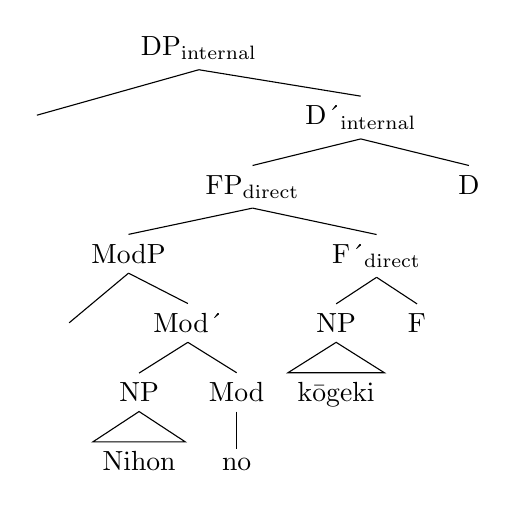
\begin{tikzpicture}[baseline=0pt, remember picture]
\tikzset{level distance=25pt, sibling distance=5pt}
 \Tree [.DP\textsubscript{internal} {} [.D´\textsubscript{internal} [.FP\textsubscript{direct} [.ModP {} [.Mod´ [.NP \edge[roof]; Nihon ] [.Mod no ] ] ] [.F´\textsubscript{direct} [.NP \edge[roof]; kōgeki ] F ] ] D ]]
\end{tikzpicture}

For arguments, the additional assumption will be made in Chapter \ref{RAJapanese} (and see \citealt{laenzlinger:2005:french, laenzlinger:2011:elements} on which this is based) that they have moved from a lower position, assuming the NP of the event noun is actually more complex.

\newpage

\section{Chapter summary and closing remarks}

This chapter presented the DP structure of Japanese and then discussed the internal structure of modifiers. The main insights are that the Japanese DP consists of a DP-external and a DP-internal domain and that the latter encompasses domains for indirect and direct modification. In the cartographic spirit, I claim that the DP structure presented in this study is universal. In other words, we need to assume a left periphery alongside a direct and an indirect domain in every language. An important deviation from other theories \citep{cinque:2010:adj, cinque:2020:relcl, scott:2002:stacked, laenzlinger:2005:french, laenzlinger:2011:elements, kim:2019:syntax} is that I have proposed that these domains do not encompass functional projections dedicated to specific semantic categories, in the direct domain, or relative clauses of different sizes, in the indirect domain. As further argued in Chapter \ref{discussiondirect}, this is due to cross-linguistic parametric variation. Furthermore, I spent some time discussing the left periphery and essentially suggested that we should cross-linguistically assume projections for quantifiers and focused modifiers, as well as unspecified projections. An intriguing question also concerns the nature and universality of FocP as the interaction of modifiers and focus in Japanese proves rather difficult. Furthermore, this area is subject to heavy language variation.

In the second part of this chapter, I put forth an analysis of the monomoraic elements co-occurring with Japanese non-verbal modifiers as a syntactic head. This head can select all kinds of lexical and functional elements, irrespective of word class and modification type -- direct, indirect, numeral, etc. -- and license them as attributive modifiers. Thus what is merged in the relevant projections is not a simple modifier, but a modifier selected by \textsc{mod}. I first put forth this analysis for the recalcitrant element \textsc{no} and then extended it to \textsc{i} and \textsc{na}. Problematic aspects for future research concern the fact that it is not realized once the head of IP is overt, as it needs to be shown whether other languages show a similar correlation between the realization of tense and of such a functional head, and the application to the Japanese adjective groups where we end up with two different elements spelled out as /i/.

As I have argued, the functional head \textsc{mod} is universal and this assumption, a theory on the internal structure of modifiers, only enriches our understanding of the DP further. This echoes a recent contribution of \citet{richards:2023:finding} on the category of \textit{linkers} (see also \citealt{richards:1997:comp, baker:2006:linkers, richards:2010:uttering}), but necessarily begs the question if such a head should really be assumed even for languages such as English where outside genitive-\textit{of} no specific element appears in the DP in order to license modification. I will answer this question affirmatively, but at the same time would like to point out the necessity of future research.

\chapter{Direct Modification in Japanese} \label{direct japanese}

This chapter is dedicated to direct -- that is, attributive -- modification in Japanese. Applying valid tests for direct modification, I present empirical and theoretical evidence that this type of modification does exist in this language and discuss every group of direct modifiers in detail. In the second part of this chapter, I will focus on the lack of ordering restrictions and show how this phenomenon falls out from the theory assumed here, the existence of unspecified functional projections within the direct domain. Next, I will discuss the question, why some languages (English, German) do show strict ordering in the direct domain, some do not (Japanese) and some do only partially, namely Persian and Greek. I will offer an explanation through the \textit{Generalization on Cross-Linguistic Ordering Restrictions} that offers a first approach to predict ordering within the direct domain. Finally, I discuss some remaining questions.

Many candidates for direct-only modifiers are scattered in various works (\citealt{yamakido:2000:japanese, yamakido:2005:nature, yamakido:2007:nature, ayano:2010:revisiting, watanabe:2012:direct, morita:2010:internal, morita:2011:three, morita:2013:morph, nagano:2015:RA, nagano:2016:are}, see especially \citealt{watanabe:2017:attributive, muraki:1996:imi, muraki:2009:nihongo, muraki:2012:nihongo}), that serve as a reference for this chapter. The main insights are based on the results of my corpus study (see Chapter \ref{corpusanalysis}) and supplemented with interviews with consultants.\footnote{These interviews were conducted online over Zoom in the period between May and June 2021. The procedure was as follows: I showed written examples to five native speakers and immediately asked for their judgment and feedback. Then we discussed critical points. These speakers were not trained linguists.}

\section{Introduction}

As was shown in the preceding chapter, the domain for direct modification is situated inside the DP-internal domain and hierarchically lower than the domain for indirect modification. Furthermore, it was argued that the functional projections inside the direct domain are not based on fine-grained semantic categories. The direct domain is circled in the following structure of the internal DP, repeated from the previous chapter.

%\newpage

\begin{figure}[H]
\centering

 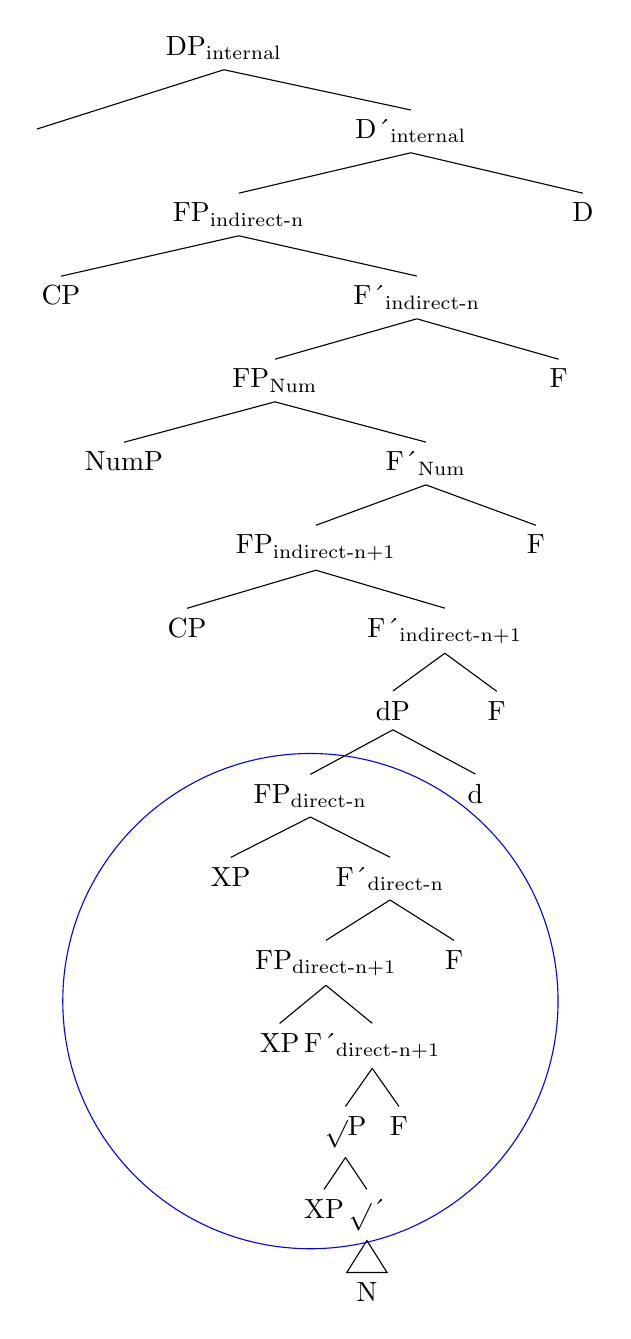
\begin{tikzpicture}[baseline=0pt, remember picture]
\tikzset{level distance=30pt, sibling distance=-5pt}
 \Tree [.DP\textsubscript{internal} {} [.D´\textsubscript{internal} [. \node (indirect1) {FP\textsubscript{indirect-n}}; CP [.\node (indirect0) {F´\textsubscript{indirect-n}}; [.FP\textsubscript{Num} NumP [.F´\textsubscript{Num} [.FP\textsubscript{indirect-n+1} \node (indirect3) {CP}; [. \node (indirect2) {F´\textsubscript{indirect-n+1}}; [.dP [. \node (direct2) {FP\textsubscript{direct-n}}; XP [. \node (direct0) {F´\textsubscript{direct-n}}; [.FP\textsubscript{direct-n+1} XP [.F´\textsubscript{direct-n+1} [.$\sqrt{}$P \node (direct1) {XP}; [.$\sqrt{}$´ \edge[roof]; N ] ] F ] ] F ] ] d ] F ] ] F ] ] F ] ] D ] ]
 \node[draw,circle,fit= (direct1) (direct2) ] [color=blue] {};
\end{tikzpicture}

 \caption{Structure of the Direct Domain in Japanese}
 \label{fig:Structure of the Direct Domain in Japanese2}
\end{figure}

\newpage

\subsection{Goals and overview}

This chapter will present the following results.

\ex. \a. Valid cross-linguistic as well as language-specific criteria for direct modification can be put forth in Japanese. The main criterion is \textit{lack of predicativity}, but this is often accompanied by other criteria such as restrictions in gradability.
\b. Japanese exhibits several groups of direct modifiers: Non-intersective modifiers, relational modifiers, direct qualitative modifiers, idiomatic modifiers, quantifiers and the language-specific group of \textit{rentaishi}.
\c. The fact that the functional projections inside the direct domain are not specified for certain semantic categories predicts the lack of ordering restrictions in linear structure.
\d. There is parametric variation as to whether a language exhibits fine-grained dedicated functional projections within the direct domain.

\subsection{Arguments against direct modification}

As mentioned in the introduction, many researchers have denied the existence of direct modification in Japanese \citep{kuno:1973:structure, hinds:1988:japanese, whitman:1981:internal, kaplan:1995:the, sproat:1991:the, baker:2003:verbal, laenzlinger:2011:elements}. And while single instances of direct modifiers have been mentioned in the literature (see \citealt{watanabe:2017:attributive}) and Japanese grammarians have long known about the category of solely attributively used lexemes, sometimes called \textit{rentaishi} (see Chapter \ref{rentaishi}), especially in syntactic research, Japanese is characterized as a language without direct modification.

The main arguments are the missing mechanism for disambiguation between direct (attributive) and indirect (predicative) modification and the lack of ordering restrictions. Some more arguments are given in \citet{baker:2003:verbal}. Building on \citet{nishiyama:1999:adj}, who argues that Japanese adjectives always project a CP layer (see Chapter \ref{copulaelements}), \citet{baker:2003:verbal} explicitly claims that direct modification is lacking in Japanese and all adjectives ``form relative-clause-like structures" \citep[19]{baker:2003:verbal}. In his framework, direct modification is an operation limited to the adjective class and denotes the modification of a noun without an additional element \citep[191]{baker:2003:cat}. A visible output of direct modification are phi-features, which Japanese lacks in general. Furthermore, he puts forth a systematic lack of non-intersectivity in Japanese and illustrates this with the equivalent of the famous \textit{beautiful dancer} example \citep{larson:1998:events}, which does not show the same ambiguity as in English between a non-intersective (subsective) and an intersective interpretation. Instead, only the intersective interpretation is available as expected under a relative clause analysis in which the intersective reading is predicatively derived (cf. \citealt{cinque:2010:adj} and Chapter \Ref{intersective}). This is shown in \ref{utsukushiibaker} based on \citet[3]{baker:2003:verbal}. %\is{intersective modifiers}

\exg. utsukushi-i kashu\\
beautiful-\textsc{i} singer \\
1. $\neq$`beautiful as a singer’ [beautiful singer] $\subseteq$ [singer] (subsective)\\
2. $\approx$ `beautiful and a singer’ [beautiful singer] = [beautiful] $\cap$ [singer] (intersective) \label{utsukushiibaker}

As will be shown below, not only are ordering restrictions not a prerequisite for direct modification in Japanese, there are also good counter arguments to the alleged absence of non-intersectivity, showcasing that none of the arguments given in the literature are convincing enough to deny the absence of direct modification in this language.

\section{Criteria and tests for direct modification} \label{testsdirect}

In order to prove that direct-only modification does exist in Japanese, it is of great importance to have specific criteria as substantial guidelines to apply to potential groups of direct modifiers. When establishing such criteria, one has to take into account not only cross-linguistic, but also language-specific aspects. Typical cross-linguistic testbeds, presented throughout the preceding chapters, are \textit{predication, gradability} and \textit{tense/inflection}. These will be looked at here, sidelining the factor \textit{ordering}, and supplemented with two language-specific factors connected to different occurrences of the copula: \textit{coordination} and \textit{co-occurrence with the canonical copula}.

\subsection{Predication} \label{test predication}

Recall from Chapter \ref{directmodifiers} that the stand-out characteristic of direct modifiers, in cartography and elsewhere, is \textit{lack of predicative use}. In English, non-verbal modifiers are licensed in predicative position via a copula, but this process is illicit with direct adjectives such as the non-intersective \textit{former} (\citealt{siegel:1976:capturing, larson:1998:events, cinque:2010:adj, cinque:2014:semantics} etc.).

Recall that Japanese \textit{na}-adjectives and \textit{no}-modifiers appear with the copular element \textsc{da} or the longer canonical copula \textsc{de-ar-u} in predicative position, the latter historically derived from the former \citep{urushibara:1993:syntactic, nishiyama:1999:adj, nakahara:2002:japanese, frellesvig:2010:history, miyama:2011:da}, as exemplified below for the \textit{na}-adjective \textit{nigiyaka} `lively’. %\is{copula}

\newpage

\ex. \ag. Ano machi-wa nigiyaka-da.\\
that city-\textsc{top} lively-\textsc{cop}\\
`That city is lively.’
\bg. Ano machi-wa nigiyaka-de-ar-u.\\
that city-\textsc{top} lively-\textsc{pred-cop-prs}\\
`That city is lively.’

\textit{i}-adjectives appear with the element \textsc{i} in predicative position which is homophonous to the output of \textsc{mod} following \textit{i}-adjectives in attributive position, as argued in the preceding chapter. I will gloss \textsc{i} in predicative position from now on as \textsc{cop}, matching the glossing for \textsc{da}.\footnote{For a precise analyses of all these elements see Chapter \ref{copulaelements}. See especially Chapter \ref{predicativei} on why \textsc{i} in predicative position is a copula as well.}

\exg. Ano machi-wa ōki-i.\\
that city-\textsc{top} big-\textsc{cop}\\
`That city is big.’

Assuming indirect modification is the only kind available in Japanese, there should be no lexemes that appear as attributive modifiers, but are unable to appear in predicative position. However, several Japanese modifiers resist predicative use, for example the \textit{na}-adjective \textit{kanzen-na} `complete' in \ref{kanzen} \citep{yamakido:2005:nature} or the \textit{no}-modifier \textit{Nihon-no} `Japan(-ese)’ in \ref{nihon direct}. %\is{direct modifiers} %\is{non-predicativity}

\ex. \label{kanzen} \ag. Max-ga kanzen-na baka-da.\\
Max-\textsc{nom} complete-\textsc{mod} idiot-\textsc{cop}\\
`Max is a complete idiot.' \hfill \citep[68]{yamakido:2005:nature}
\bg. *Ano baka-ga kanzen-da.\\
that idiot-\textsc{nom} complete-\textsc{cop}\\
(`That idiot is complete.’)

\ex. \label{nihon direct} \ag. Nihon-no kuruma\\
Japan-\textsc{mod} car\\
`Japanese car'
\bg. *Kono kuruma-wa Nihon-da.\\
this car-\textsc{top} Japan-\textsc{cop}\\
(`This car is Japanese.’)

Importantly, one needs to take into account other exponents of the copula such as \textsc{desu} (and the forms analyzed in Chapter \ref{copula}), which is a more polite version of \textsc{da}. Accordingly, the two instances of the copula behave alike. In instances where \textsc{da} is impossible, \textsc{desu} is as well.\footnote{This element, which can never appear in attributive position, will be discussed in Chapter \ref{desu} where it will be depicted as a combination of the predicative copula, the polite form of the dummy copula and a tense marker for non-past. For now, I will apply the gloss \textsc{cop.pol} to highlight its function as a polite copula.} %\is{copula}

\newpage

\ex. \ag. *Ano baka-ga kanzen-desu.\\
that idiot-\textsc{nom} complete-\textsc{cop.pol}\\
(`That idiot is complete.’; polite)
\bg. *Kono kuruma-wa Nihon-desu.\\
this car-\textsc{top} Japan-\textsc{cop.pol}\\
(`This car is Japanese.’; polite)

Such examples have provided the main motivation for authors such as \cite{yamakido:2005:nature} to argue against a universal analysis of Japanese modifiers as indirect. \textit{Predication}, especially its absence, will be used as the main criterion to check for direct modification verified via the occurrence of the copula forms \textsc{da} and \textsc{i}. %\is{copula}

It should be noted here that in Japanese, seemingly direct modifiers can, in specific instances, appear with the copula. First, predicative use can be facilitated easily in contrastive statements. An example is the following (and see \citealt{hoshi:2002:kaynean, shimada:2018:relational}).

\exg. Kono kuruma-ja-na-ku-te, ano kuruma-ga Nihon-da.\\
this car-\textsc{pred.top-neg-pred-ger} that car-\textsc{nom} Japan-\textsc{cop}\\
`Not this car, that car is Japanese.’ \label{kurumajanakute}

Here, the direct-only modifier \textit{Nihon} `Japan(-ese)’ seemingly appears in predicative position. See also the following example reported in \citet{hoshi:2002:kaynean} who argues against a direct status of \textit{omoigakena-i} `unexpected’, which \citet{yamakido:2005:nature} argues to be direct.

\exg. Kono kyaku ja-na-ku-te, ano kyaku-ga omoigakena-i no-da.\\
this guest \textsc{pred.top-neg-rky-ger} that guest-\textsc{nom} unexpected-\textsc{cop} \textsc{emp-cop}\\
`Not this visitor, that visitor is unexpected.' \\ \null \hfill \citep[11]{hoshi:2002:kaynean}

In the literature on relational adjectives, many such instances in which otherwise non-predicative relational adjectives appear in predicative position are reported, including class shift and the availability of a \textit{kind}-reading. This instances are referred to as \textit{adjective stranding} (\citealt{levi:1978:syntax, mcnally:2004:relational, nagano:2018:conversion}; see Chapter \ref{RA}). Another typical way to achieve predicative occurrence involves contrastive use, as in the Japanese examples, shown for English below. %\is{adjective stranding}

\ex. Her infection turned out to be bacterial, not viral. \null \hfill \citep[254]{levi:1978:syntax} \label{viral stranding}

In \ref{viral stranding}, the relational adjective \textit{viral} is used predicatively. In a context-neutral sentence, such a use is significantly degraded.

\ex. ??Her infection is viral.

According to \citet[255]{levi:1978:syntax}, in such instances the second noun is elided under identity at a late stage in the derivation. One piece of evidence she puts forth is that the two instances, the noun and the modifier, must be established as a set. The first instance of the noun then licenses the deletion of the second instance under phonological identity. This means \ref{viral stranding} is derived from \ref{stranded analysis}.

\ex. Her infection turned out to be (a) bacterial \st{infection}, not (a) viral \st{infection}. \null \hfill \citep[254]{levi:1978:syntax} \label{stranded analysis}

Applying the data to Japanese, this means that the underlying construction of \ref{kurumajanakute} is \ref{kuruma analysis}. Since no overt modifier is present, the syntactic head \textsc{mod} is deleted alongside.

\exg. Kono kuruma-ja-na-ku-te, ano kuruma-wa Nihon-\st{no} \st{kuruma} da.\\
this car-\textsc{pred.top-neg-pred-ger} that car-\textsc{top} Japan-\textsc{mod} car \textsc{cop}\\
`Not this car, that car is \st{a} Japanese \st{car}.’ \label{kuruma analysis}

Evidence for this claim comes from the fact that this sentence is even more natural when the noun \textit{Nihon} `Japan(-ese)’ is followed by a so-called \textit{bound marker}, a nominal suffix which specifies the denotation of the noun \citep{nagano:2016:are, shimada:2018:relational}. This in turn makes it easier for the two nouns to be established as a set and facilitates predicate use (see Chapter \ref{Ra japanese predicative} and appendix A for more on bound markers.) %\is{bound markers}

\exg. Kono kuruma-wa Nihon-sei-d-a.\\
this car-\textsc{top} Japan-produce \textsc{pred-cop.prs}\\
`This car is Japanese.’ (Lit. `is Japan-produce’)

Furthermore, the copula can oftentimes function as a placeholder for other verbs. This is the famous \textit{eel-construction} or \textit{unagi-bun} coined by \citet{okutsu:1978:boku}. In \ref{eel-sentence}, the copula \textsc{da} appears, but is understood as a lexical verb, for example \textit{tabe} `to eat’, depending on the context. Semantically, it does not express an equative relation between \textit{I} and \textit{eel}. %\is{eel-construction}

\exg. Kare-wa sakana-wo tabe-ta. Boku-wa unagi-da.\\
he-\textsc{top} fish-\textsc{acc} eat-\textsc{acc} I-\textsc{top} eel-\textsc{cop}\\
`He ate a fish. I ate/had (the) eel.’ (Lit.: `I am eel.’) \label{eel-sentence}

This means that, provided the appropriate context, formerly non-predicative lexemes can become acceptable in predicative position. \textit{Unagi}-constructions are very productive and usually involve a noun directly preceding the copula \citep[23–29]{okutsu:1978:boku}. Since many of the relational modifiers discussed here are nominal in nature, it is no surprise that they can appear in such constructions. In other words, it is oftentimes not clear if we are dealing with a proper predicative phrase in the relevant instances. In the discussion at the end of this chapter, I will furthermore discuss some indirect features of direct modifiers in Japanese.

\subsection{Gradability} \label{gradability}

A further typical characteristic often observed with direct modifiers and generally related to their less complex nature is \textit{non-gradability}, the inability to express a degree. Gradability can be expressed through modification by degree heads \ref{toolarge}, degree adverbs \ref{verylarge} or the formation of the comparative or superlative \ref{thanlarge} (cf. \citealt{baker:2003:cat}). %\is{gradability}

\ex. \a. a too large building \label{toolarge}
\b. a very large building \label{verylarge}
\c. a larger building than Tokyo Tower \label{thanlarge}

It is a general property of the word class \textit{adjective} to express a degree, although not all adjectives are equally freely gradable \citep[70–74]{dixon:2010:grammatical}. A restriction in gradability is a central characteristic of both, the group of relational \ref{relational, non-gradable} and non-intersective adjectives \ref{nonintersective, non-gradable} in most European languages (see references in the preceding chapter). %\is{non-gradable modifiers}

\ex. \label{relational, non-gradable} \a. *very / *too /*more nuclear energy
\b. *very / *too / *more American attack

\ex. \label{nonintersective, non-gradable} \a. *very / *more former minister
\b. *totally present editor

The semantic approach to gradability makes use of scale structures \citep{kennedy:2005:scale, kennedy:2007:vagueness, morzycki:2012:adj}. Gradable adjectives are understood as \textit{relative} in contrast to \textit{absolute} or \textit{totally closed scale} adjectives. Only the former can be modified by so-called \textit{proportional modifiers}, including the common degree adverb \textit{very}, whereas the latter allow modification via \textit{endpoint-oriented modifiers} \citep{kennedy:2005:scale}, also called \textit{modifiers of extension} \citep{fabregas:2014:adjectival} such as \textit{completely}, denoting a maximum scale, or \textit{slightly}, denoting a minimum scale \citep[355]{kennedy:2005:scale}. The term \textit{non-gradable modifier} will be used in this book to denote those modifiers that cannot be combined with any degree adverb and do not have access to comparative-formation. %\is{non-gradable modifiers}

It is important to note that lack of gradability does not automatically entail lack of predication and that gradability is not a sufficient criterion for direct modification, yet often an accompanying one. Absolute adjectives such as \textit{pregnant} or \textit{bent}, despite restrictions in gradability, can productively appear in predicative position in English. \citet{cinque:2010:adj} also provides examples of some non-intersective adjectives in English (and Italian and Bulgarian) that can be combined with degree adverbs.

\ex. the most probable winner \hfill \citep[47]{cinque:2010:adj}

Gradability in Japanese is expressed via the particle \textit{yori(-mo)} `than' and the optional adverb \textit{motto} `more' or by various degree adverbs (see Chapter \ref{intro japanese}). The most prototypical one is \textit{totemo} `very’, the equivalent of the proportional modifier \textit{very} in English. Equivalents of endpoint modifiers are the maximum-standard degree adverbs \textit{kanzenni} and \textit{mattaku}, both `completely’, and the minimum-standard degree adverb \textit{wazukani} `slightly‘ (cf. \citealt{oshima:2019:gradability}). %\is{endpoint modifiers}

It is often claimed that \textit{no}-modifiers are non-gradable in general \citep{kato:2003:nihongo, morita:2011:three, morita:2013:morph}. And while most are incompatible with the degree adverb for relative comparison \textit{totemo} `very’ \Ref{totemo mumei}, many are compatible with the adverb \textit{kanari} `quite’, as well as the maximum- and minimum-standard degree adverbs mentioned above \ref{kanari mumei}.\footnote{A reviewer points out that example \ref{wazukani mumei-no} is pragmatically odd, as, indeed, the standard way to express this notion would be a combination along the lines of `very famous'. Nevertheless, this example serves an illustrative illustration purpose.}%\is{endpoint modifiers}

\exg. ??totemo mumei-no haiyū\\
very unknown-\textsc{mod} actor\\
`very unknown actor’ \label{totemo mumei}

\ex. \label{kanari mumei} \ag. kanari mumei-no haiyū\\
quite unknown-\textsc{mod} actor\\
`quite unknown actor'
\bg. kanzenni / mattaku mumei-no haiyū\\
completely / completely unknown-\textsc{mod} actor\\
`completely unknown actor'
\cg. wazukani mumei-no haiyū\\
slightly unknown-\textsc{mod} actor\\
`slightly unknown actor' \label{wazukani mumei-no}

Also note that many \textit{no}-modifiers, for example \textit{mumei-no} `unknown’, can productively appear inside a comparative construction with the comparative particle \textit{yori} `than’.

\newpage

\exg. Tanaka-san-yori (motto) mumei-no haiyū-to at-ta.\\
Tanaka-Mr.-than more unknown-\textsc{mod} actor-\textsc{com} meet-\textsc{pst}\\
`I met with a more unknown actor than Mr. Tanaka.’

Although this shows that gradability is restricted for \textit{no}-modifiers, as also corroborated in the study of \citet{oshima:2019:gradability} in which the authors judged only 22.25\% of the 200 most used \textit{no}-modifiers on the BCCWJ to be gradable,\footnote{They followed up on their judgment with a questionnaire survey and identified only 8.28\% of the 169 \textit{no}-modifiers they considered as gradable on a relative scale, thus with \textit{totemo} \citep[29]{oshima:2019:gradability}.} there are some \textit{no}-modifiers which are compatible with relative degree adverbs of the type \textit{totemo} `very’, although only a few. See \ref{gradable no} and \citet{oshima:2019:gradability}, as well as their data set, for more examples. %\is{no-modifiers}

\ex. \label{gradable no} \ag. totemo totsuzen-no henka\\
very sudden-\textsc{mod} change\\
`a very sudden change’
\bg. yori ōgata-no fune\\
more large.size-\textsc{mod} ship\\
`a ship of a larger size’ \null \hfill \citep[16]{oshima:2019:gradability}

Nevertheless, most non-predicative modifiers in Japanese resist gradability across the board, as exemplified for the non-intersective modifier \textit{shōrai-no} `future’ in \ref{shorai non-gradable} and to be discussed in the following.

\exg. *totemo shōrai-no daitōryō\\
very future-\textsc{mod} prime.minister\\
(`a very future prime minister’) \label{shorai non-gradable}

\subsection{Tense and inflection} \label{test tense}

The absence of tense information is another criterion that differentiates direct from indirect modifiers. This can be easily illustrated with German where adjectives can be used attributively together with a copula appearing as a as prenominal participle, a case of a reduced relative clause (\citealt[203]{cinque:2020:relcl}; \citealt{krause:2001:rrc, douglas:2016:syntactic, harwood:2018:rrc}). This is shown in \ref{ehemalig weis} for the adjective \textit{weiß} `white’, which can be used as a predicate. The non-intersective adjective \textit{ehemalig} `former’, on the other hand, can never appear together with an inflected copula, as it can never appear with the copula in the first place \ref{ehemalig fruher}, highlighting its direct status. %\is{tense}

\exg. das (früher einmal) weiß gewesene Hemd (German)\\
the earlier once white be.\textsc{pst.ptcp} shirt\\
`the shirt which was (once) white’ \label{ehemalig weis}

\exg. *der ehemalig gewesene Präsident (German)\\
the former be.\textsc{pst.ptcp} president\\
(`the was former president’) \label{ehemalig fruher}

As shown in Chapter \ref{internalstructure}, Japanese modifiers can inflect for past DP-internally, but this is impossible for non-predicative modifiers such as \textit{kanzen-na} `complete’ \Ref{kanzendatta}.\footnote{That non-intersective adjectives cannot inflect for past also applies in Korean as shown by \citet[164]{kang:2005:adj}.}

\exg. *ano kanzen-d-at-ta baka\\
that complete-\textsc{pred-cop-pst} idiot\\
(`that idiot who was complete’) \label{kanzendatta} \null \hfill \citep[109]{ayano:2010:revisiting}

From a theoretical angle, these facts fall out naturally. The structure of direct modifiers is less complex and no IP layer is present, hence no overt tense can be expressed. In a nutshell, whereas the endings \textsc{de-ar-u}, \textsc{d(e)-at-ta} and \textsc{k-at-ta} always carry tense information, this is not obligatorily the case for \textsc{i}, \textsc{na} and \textsc{no}. As shown in Chapter \ref{indirect mod}, this only applies when they are indeed part of a relative clause (see also \citealt[793]{watanabe:2017:attributive}). Direct modifiers can therefore never, instead of the monomoraic endings, co-occur with the complex copula forms.

\subsection{Co-occurrence with other copula forms} \label{copula}

I will now discuss two rather language-specific tests. These correlate with the inability of predicative use as they look at co-occurrence with two different exponents of the copula, namely the canonical copula \textsc{de-ar-u} and coordination forms. %\is{copula}

\subsubsection{The Canonical Copula \textit{de-ar-u}}

The complex form \textsc{de-ar-u} is usually called the \textit{standard} or \textit{canonical} copula \citep{urushibara:1993:syntactic, nishiyama:1999:adj, nakahara:2002:japanese}. Recall (for instance from Chapter \ref{intro japanese}) that this canonical copula co-occurs with \textit{na}-adjectives and \textit{no}-modifiers and that it is not only mutually exclusive with the copula \textsc{da}, but also with the attributive exponents of \textsc{mod}, namely \textsc{na} and \textsc{no}. This is repeated for convenience for the \textit{na}-adjective \textit{nigiyaka-na} `lively’ \ref{nigiyaka convenience} and the \textit{no}-modifier \textit{shujinkō} `main protagonist’ \ref{taro convenience}.\footnote{For \textit{i}-adjectives, in order to paraphrase \textit{i} with the corresponding \textit{ku-ar-u}, the right context is needed. See Chapter \Ref{copulaelements}.} %\is{copula}

\ex. \label{nigiyaka convenience} \ag. nigiyaka-na machi\\
lively-\textsc{mod} city\\
\bg. nigiyaka-de-ar-u machi\\
lively-\textsc{pred-cop-prs} city\\
`a city which is lively’

\newpage

\ex. \label{taro convenience} \ag. Tarō-ga shujinkō-no monogatari\\
Taro-\textsc{nom} main.protagonist-\textsc{mod} story\\
\bg. Tarō-ga shujinkō-de-ar-u monogatari\\
Taro-\textsc{nom} main.protagonist-\textsc{pred-cop-prs} story\\
`story in which Taro is the main protagonist' \\ \null \hfill \citep[66]{watanabe:2010:notes}

That \textsc{no} is not (always) an instance of the copula can be shown in the following minimal pair in which \textsc{no} can yield both an equative, as well as a possessive meaning, whereas \textsc{de-ar-u}, on the other hand, only causes the nominal modifier to have an equative reading, highlighting its predicative nature (see also \citealt{kato:2003:nihongo} among others). %\is{copula} %\is{coordination}

\exg. sensei-no tomodachi\\
teacher-\textsc{mod} friend\\
1. $\approx$ `(my) friend who is a teacher' (equative)\\
2. $\approx$ `friend of the teacher' (possessive) \label{senseino}

\exg. sensei-de-ar-u tomodachi\\
teacher-\textsc{pred-cop-prs} friend\\
1. $\approx$ `(my) friend who is a teacher' (equative)\\
2. $\neq$`friend of the teacher' (possessive)

Cross-linguistically, there is agreement, that the copula is a licensor of non-verbal elements in predicative position, thus linking the predicate to its subject, and that it is in essence meaningless (\citealt[1–6]{arche:2019:main}, see \citealt{moro:1997:raising, moro:2000:dynamic, bowers:2002:pred} among others for historical overview). The appearance of the copula itself is thus strongly linked to indirect modification. On the other hand, ``non-paraphrasability with a copular construction" is a sign of direct modification \citep[291–292]{alex:2007:nounphrase}. %\is{copula}

This means that when direct-only \textit{na}-adjectives and \textit{no}-modifiers are used attributively, \textsc{de-ar-u}, or \textsc{d(e)-at-ta}, should never occur instead of the different outputs of \textsc{mod} (see also \citealt{ayano:2010:revisiting}). This is shown below for a direct \textit{na}-adjective \ref{kanzen no cop} and a direct \textit{no}-modifier \ref{nihon no cop}. Note that this fact relates again to the lack of tense of direct modifiers and their smaller structure which does not contain projections for these complex elements. %\is{copula}

\exg. *ano kanzen-de-ar-u baka\\
that complete-\textsc{pred-cop-prs} idiot\\
(`that idiot who is complete’) \null \hfill \citep[108]{ayano:2010:revisiting} \label{kanzen no cop}

\exg. *Nihon-de-ar-u kuruma\\
Japan-\textsc{pred-cop-prs} car\\
(`car which is Japanese’) \label{nihon no cop}

\subsubsection {The Coordinative Form \textit{de}} \label{coordination copula}

Besides the canonical and the polite form of the copula, direct-only modifiers also cannot co-occur with the coordinative form of the copula \textsc{de}. They are even illicit in coordinative constructions in which the first conjunct bares the copula form. %\is{coordination}

In Japanese, different word classes use different methods of coordination, meaning there is no universal coordinator at the word level similar to English \textit{and}. Nouns are connected via the comitative/conjunction postposition \textsc{to} (or the postposition \textsc{ya} for inexhaustive coordination).\footnote{The comitative postposition -\textsc{to} further differs from the other elements to be reviewed in that it can also appear after the last noun in a list format and even together with (case) particles. See examples and discussion in \citet{kuno:1973:structure} and \citet{hiraiwa:2014:constraining} against \citet{tatsumi:2018:splitting}.}

\exg. hon-to shinbun\\
book-and newspaper\\
`books and newspapers' \\ \null \hfill nominal coordination, exhaustive

Verbs (and generally inflecting word classes), on the other hand, are coordinated via the suffix -\textsc{te}, which implies a consecution of actions and possibly additional connections between two clauses, for instance causality.\footnote{-\textsc{te} also functions as an aspectual marker and is often glossed \textsc{prog} or \textsc{ger(und)}. I will adopt the label \textsc{ger}, but note that this element has nothing to do with nominalization \textit{per se}. See \citet{hasegawa:1996:study, mihara:2013:tekei, nakatani:2013:predicate, nakatani:2016:complex}.} -\textsc{te} attaches to the nominalization form (\textit{renyōkei}) and can undergo various phonological assimilation processes. The element \textit{koron-de} in \ref{koronde} consists of the verb \textit{korob} `to fall’, inflected to the nominalization form \textit{korobi}, to which -\textsc{te} is added and phonological assimilation takes place.\footnote{The combination /bi te/ was present still in Classical Japanese, but has become /nde/ as a result of historical sound change (\textit{onbin}). This form can now be interpreted as analytical. In Modern Japanese, the voiced variant /de/ of the coordinative form appears after all consonant-stem verbs ending in a nasal or a voiced obstruent. A similar phonological assimilation process, gemination, happens before the past marker -\textsc{ta} \citep{ito:2015:word}.} The nominalization form of vowel-stem verbs, such as \textit{tabe} `to eat’, is syncretic with the infinitival form and the coordinative marker is always just /te/ as shown in \ref{tabete}. %\is{coordination}

\ex. \ag. Ken-wa koron-de nai-ta.\\
Ken-\textsc{top} fall-\textsc{ger} cry-\textsc{pst}\\
`Ken fell down and cried.’ \\ \null \hfill verbal coordination, consonant verb \citep[357]{hiraiwa:2012:mechanism} \label{koronde}
\bg. Bangohan-wo tabe-te o-furo-ni hait-ta.\\
dinner-\textsc{acc} eat-\textsc{ger} \textsc{hon}-bath-\textsc{ill} enter-\textsc{pst}\\
`(I) ate dinner and (afterwards) took a bath.' \\ \null \hfill verbal coordination, vowel verb \label{tabete}

\textit{i}-adjectives are coordinated via the same suffix, which attaches to the inflection form /ku/, in Chapter \ref{copulaelements} argued to be the predicative copula. In more elaborate contexts, bare /ku/ (the bare predicative copula) can be used for coordination, although this is highly restricted and does rarely appear in spoken Japanese. See below. %\is{copula} %\is{coordination}

\ex. \ag. taka-ku-te mazu-i okashi\\
expensive-\textsc{pred-ger} unpleasant-\textsc{mod} sweet\\
`expensive and terrible sweets' \\ \null \hfill \textit{i}-adjective, coordinated with -\textsc{te}
\bg. taka-ku mazu-i okashi\\
expensive-\textsc{pred} unpleasant-\textsc{mod} sweet\\
`expensive and terrible sweets' \\ \null \hfill \textit{i}-adjective, coordinated without -\textsc{te}

When \textit{na}-adjectives and \textit{no}-modifiers appear as the first conjunct, they exhibit the element \textsc{de}, exemplified below for a \textit{na}-adjective.\footnote{The second conjunct, the modifier directly preceding the noun can never appear with -\textsc{te/de}.

\par

\ex. \ag. *mazu-i taka-ku-te okashi\\
unpleasant-\textsc{mod} expensive-\textsc{pred-ger} sweet\\
\bg. *benri-na jōbu-de kuruma\\
practical-\textsc{mod} robust-\textsc{pred} car\\

\par


A reviewer asks why a conjecture in which a coordinated modifier carries \textsc{mod} in addition to the coordinative form of the copula, so for instance *\textit{benri-de-na}, is ruled out. I hypothesize that this is for the same reason why combinations of the canonical copula form \textsc{de aru} and any form of the copula are ruled out, although perhaps more opaque. It seems that overt realization of the head of PredP, which is the predicative copula as addressed in Chapter \ref{chapter pred} blocks the overt occurrence of \textsc{mod} as well, same as the head of IP.}

\exg. benri-de jōbu-na kuruma\\
practical-\textsc{pred} robust-\textsc{mod} car\\
`a practical and robust car'

This element is homophonous to the allophone /de/, the voiced version of the coordination suffix \textsc{te} after verbs ending in a voiced obstruent or nasal. They might look like the same element, however, they should be kept apart and \textsc{de} co-occurring with \textit{na}-adjectives and \textit{no}-modifiers is, in fact, an instance of the copula. Several pieces of evidence for this are given in \citet{hiraiwa:2012:mechanism}, and see \citet{bloch:1970:bloch}. The first piece of evidence comes from distributional patterns. As the predicative copula \textsc{da} is mutually exclusive with the canonical copula \textsc{de-ar-u} reviewed above, the coordinative copula \textsc{de} corresponds also to a longer form: The coordinative form of the canonical copula \textsc{de-at-te}. Note the morphological setup, shown in \ref{set up de-at-te}, in which, again, the suffix -\textsc{te} is added to the nominalization form.\footnote{The historical nominalization form of verbs of the \textit{aru}-paradigm (which \textit{ar}- is the prime member of) was /ri/. Phonological assimilation has led to deletion of /r/ and gemination of /t/, so to a sound change from /ri te/ to /tte/. Again, the bare nominalization form \textsc{de-ar-i} can be used for coordination and behaves essentially like \textsc{de-at-te}.} %\is{copula} %\is{coordination}

%\newpage

\exg. benri-de-at-te jōbu-na kuruma\\
practical-\textsc{pred-cop-ger} robust-\textsc{mod} car\\
`a car that is practical and robust' \label{set up de-at-te}

This means that both, \textsc{de} and \textsc{de-at-te}, as well as \textsc{to} appear in contexts where nouns are coordinated. However, the former two elements are used for \textit{clausal coordination} of a \textit{no}-modifier with another modifier, in the sense that both exhibit predicativity. \textsc{to} can never be used in clausal instances. This is illustrated below (and cf. examples in \citealt[363]{hiraiwa:2012:mechanism}). %\is{copula} %\is{coordination}

\ex. \ag. Hanako-wa gakusei-de (-at-te) Nihon-jin da.\\
Hanako-\textsc{top} student-\textsc{pred} (-\textsc{cop}-\textsc{ger}) Japan-person \textsc{cop}\\
`Hanako is a student and Japanese.’
\bg. Hanako-wa gakusei-de (-at-te) hon-wo yo-mu koto-ga suki-da\\
Hanako-\textsc{top} student-\textsc{pred} (-\textsc{cop}-\textsc{ger}) book-\textsc{acc} read-\textsc{prs} \textsc{comp-nom} like-\textsc{cop}\\
`Hanako is a student and likes reading books.’
\cg. *Hanako-wa gakusei-to hon-wo yo-mu koto-ga suki-da\\
Hanako-\textsc{top} student-and book-\textsc{acc} read-\textsc{prs} \textsc{comp-nom} like-\textsc{cop}\\
(`Hanako is a student and likes reading books.’)

More evidence comes from the connective element \textit{katsu}, which \citet[364]{hiraiwa:2012:mechanism} calls a \textit{sentential conjunction marker}. \textit{Katsu} necessarily adds an additional state of affairs, is restricted to written speech and can only follow nouns, \textit{na}-adjectives and verbs in their nominalization form. That it must express a predication relation is illustrated in the following sentence, where a pure coordination reading, in which the person under description is the teacher of both Ken and Naomi, cannot be achieved. The only possible interpretation is `this person is Ken and this person is also Naomi's teacher’.\footnote{This sets \textit{katsu} clearly apart from \textit{shi} which has to appear with verbs inflected for tense. See also \citet{fenger:2020:words}.} %\is{copula} %\is{coordination}

\exg. *Kono hito-wa Ken katsu Naomi-no sensei-da.\\
this person-\textsc{top} Ken katsu Naomi-\textsc{mod} teacher-\textsc{cop}\\
Under interpretation: `This person is Ken's and Naomi's teacher.’

The same holds true of -\textsc{de}. This element also shows a restriction to clausal, that is predicative, contexts, giving further evidence that it is connected to indirect modification.

%\newpage

\exg. Kono hito-wa Ken-de Naomi-no sensei-da.\\
this person-\textsc{top} Ken-\textsc{pred} Naomi-\textsc{mod} teacher-\textsc{cop}\\
1. $\neq$ `This person is Ken's and Naomi's teacher.’\\
2. only: $\approx$ `This person is Ken, and this person is Naomi’s teacher.’

The predicative, nature of \textsc{de} can be further highlighted via its interaction with \textit{katsu}. If two entities are predicated on one noun, one of these elements has to appear, or both. The meaning is unchanged. %\is{copula} %\is{coordination}

\ex. \ag. Kono hito-wa Ken-no sensei *(katsu) Naomi-no sensei-da.\\
this person-\textsc{top} Ken-\textsc{mod} teacher \textsc{katsu} Naomi-\textsc{mod} teacher-\textsc{cop}\\
\bg. Kono hito-wa Ken-no sensei-*(de) Naomi-no sensei-da.\\
this person-\textsc{top} Ken-\textsc{mod} teacher-\textsc{pred} Naomi-\textsc{mod} teacher-\textsc{cop}\\
\cg. Kono hito-wa Ken-no sensei-de (katsu) Naomi-no sensei-da.\\
this person-\textsc{top} Ken-\textsc{mod} teacher-\textsc{pred} \textsc{katsu} Naomi-\textsc{mod} teacher-\textsc{cop}\\
`This person is Ken's teacher and (also) Naomi's teacher.’ \\ \null \hfill \citep[364–365]{hiraiwa:2012:mechanism}

This shows that, clearly, \textsc{de} is an instance of the copula. This in turn predicts that non-predicative modifiers are banned from coordination with \textsc{de} (and also \textsc{de-at-te}), which is borne out, as illustrated below for the non-predicative \textit{na}-adjective \textit{kanzen-na} `complete’ and the \textit{no}-modifier \textit{Nihon-no} `Japan(-ese)’. %\is{direct modifiers}

%\newpage

\ex.\ag. *Max-ga kanzen-de baka-da.\\
Max-\textsc{nom} complete-\textsc{pred} idiot-\textsc{cop}\\
\bg. *Max-ga kanzen-de-at-te baka-da.\\
Max-\textsc{nom} complete-\textsc{pred-cop-ger} idiot-\textsc{cop}\\
(`Max is complete and Max is an idiot.’)

\ex. \ag. *Nihon-de jōbu-na kuruma\\
Japan-\textsc{pred} robust-na car\\
\bg. *Nihon-de-at-te jōbu-na kuruma\\
Japan-\textsc{pred-cop-ger} robust-na car\\
(`a Japanese and robust car’)

An even more striking observation is that non-predicative modifiers cannot even appear in coordinative structures inside the DP as the second conjunct, regardless of whether the modifier to their left can appear in predicative position or not. As shown in \ref{kirei second conjunct}, although \textit{kirei-na} `beautiful’ can appear predicatively and can be coordinated, it cannot appear in coordination structures with a non-predicative modifier such as \textit{Chūgoku-no} `Chinese’, causing the DP to be ungrammatical.

\exg. *kirei-de Chūgoku-no kabin\\
beautiful-\textsc{pred} China-\textsc{mod} vase\\
(`a beautiful and Chinese vase’) \label{kirei second conjunct}

\section{Direct modifiers in Japanese}

The following diagnostics for direct modifiers in Japanese were established in the previous section: \textit{Lack of predication, non-gradability, lack of tense/inflection, no co-occurrence with canonical copula, lack of coordination}. These tests will help to identify the relevant groups of direct modifiers. I will start with a discussion on those groups of direct modifiers that are cross-linguistically attested, and finally come to the language-specific group of \textit{rentaishi}. %\is{direct modifiers}

Recall that with the notion \textit{direct-only}, I refer to those modifiers that truly can never appear in predicative position. For many of the modifiers discussed in the following pages, predicative use, and this extends to the other characteristics, can be achieved. For example, the relational modifier \textit{Chūgoku} is direct when denoting an origin, `Chinese, from China’. Its principal meaning, denoting something related to the country `China’, however, is possible in predicative position, which is why modifiers of \textsc{nationality} are often attested in the corpus in combination with the copula. As mentioned, group 5 of the data set contains some modifiers for which predicative use is marginal, but nevertheless attested, meaning those are not direct-only. Reflecting the obvious skew, which needed to be at least 5$>$1, towards attributive use, I classified such modifiers as \textit{prototypically attributive} and also sorted them to this group. Cf. Chapter \ref{corpusanalysis}.

\subsection{Non-intersective modifiers} \label{non-intersective Japanese}

A cross-linguistically prominent group of direct-only modifiers, outlined in Chapter \ref{intersective}, are non-intersective modifiers of the type \textit{former}. Those are characterized by the missing set intersection between their denotation and that of the noun they modify and can be sub-classified into \textit{truly non-intersective modifiers}, which can never be used predicatively, \textit{subsective} modifiers, which can be used predicatively but then exhibit an intersective meaning, \textit{privative} modifiers and \textit{adnominal degree morphemes} \citep{vendler:1957:verbs, bolinger:1967:adj, larson:1998:events, morzycki:2016:mod}.

\subsubsection{Non-Intersective Adjectives}

Several non-intersective adjectives in Japanese are presented in the PhD thesis of \citet{yamakido:2005:nature} (cf. also \citealt{yamakido:2000:japanese, yamakido:2007:nature}), who argues explicitly against a unified relative clause analysis of Japanese adjectives, and in \citet{ayano:2010:revisiting}. The authors show that ambiguous examples of the type \textit{old friend} in English are disambiguated via two separate lexemes in Japanese. The \textit{i}-adjective \textit{furu-i} can be translated as `old’, but cannot be used to denote the age of a human entity. In other words, it only gives a subsective reading when modifying human nouns while its intersective interpretation is blocked \citep[66–67]{yamakido:2005:nature}. In order to denote a person's age, other lexemes have to be used, such as \textit{kōrei-na} `old’. This is illustrated below with the relevant notation.\footnote{As \citet[511, Fn. 7]{watanabe:2012:direct} notes, the phrase \textit{furu-kara-no} old-from-\textsc{mod} `from a long time ago' might be a better and more natural alternative to \textit{furu-i}. See also \citet[155–156]{tatsuki:2009:nihongo}.} %\is{non-intersective modifiers}

\exg. furu-i tomodachi\\
old-\textsc{mod} friend \null \hfill \citep[81]{yamakido:2005:nature}\\
1. $\approx$ `long-time friend’ [furu-i tomodachi] $\subseteq$ [tomodachi] (subsective)\\
2. $\neq$ `aged friend’ [furu-i tomodachi] = [furu-i] $\cap$ [tomodachi] (intersective)

\exg. kōrei-na tomodachi\\
old-\textsc{mod} friend \null \hfill \citep[67]{yamakido:2005:nature}\\
1. $\neq$ `long-time friend’ [kōrei-na tomodachi] $\subseteq$ [tomodachi] (subsective)\\
2.$\approx$ `aged friend’ [kōrei-na tomodachi] = [kōrei-na] $\cap$ [tomodachi] (intersective)

Lack of intersective interpretation suggests lack of predicative use, which in turn suggests direct modification status \citep{larson:1998:events, cinque:2010:adj}. As expected, this adjective cannot be used predicatively, at least not with human entities (cf. \citealt[67]{yamakido:2005:nature}). %\is{non-intersective modifiers}

\exg. *Watashi-no tomodachi-wa furu-i.\\
I-\textsc{mod} friend-\textsc{top} old-\textsc{cop}\\
(`My friend is old (aged).’)

Another case of ambiguity resolution presents itself in the \textit{beautiful dancer} example. \citet[3]{baker:2003:verbal} is right when he says that the direct equivalent \textit{utsukushi-i / kirei-na kashu} `beautiful singer’ only has an intersective reading, denoting the beauty of a person irrespective of their singing skills. However, other lexemes allow only a non-intersective, that is a subsective, interpretation of beauty pertaining to the dancing or singing skills of a person. Such lexemes are \textit{takumi-na} `skillful \citep[101, Fn. 2]{ayano:2010:revisiting}, \textit{migoto-na} \citep[786]{watanabe:2017:attributive}, which can be translated as `beautiful’, but can only be used with reference to events, or \textit{suteki-na} `wonderful'. This contrast is shown below. %\is{ambiguity resolution}

\exg. utsukushi-i kashu\\
beautiful-\textsc{mod} singer \null \hfill \citep[3]{baker:2003:verbal}\\
1. $\neq$ `beautiful as a singer’ [beautiful singer] $\subseteq$ [singer] (subsective)\\
2. $\approx$ `beautiful and a singer’ [beautiful singer] = [beautiful] $\cap$ [singer] (intersective)

\exg. Hanako-wa takumi-na / migoto-na / suteki-na kashu-da.\\
Hanako-\textsc{top} skilfull-\textsc{mod} / beautiful-\textsc{mod} / wonderful-\textsc{mod} singer-\textsc{cop}\\
1. $\approx$ `beautiful as a singer’ [takumi-na kashu] $\subseteq$ [kashu] (subsective)\\
2. $\neq$ `beautiful and a singer’ [takumi-na kashu] = [takumi-na] $\cap$ [kashu] (intersective)

This ambiguity resolution via two different lexemes points towards the fact that one is a direct, and the other an indirect modifier. Similar ambiguity resolutions have been observed in Korean \citep[161]{kang:2005:adj}, and German \citep[69]{maienborn:2020:revisiting}. %\is{german, korean}

Japanese also has truly non-intersective adjectives, among those the \textit{i}-adjective \textit{omoigakena-i} `unexpected' and the \textit{na}-adjective \textit{kanzen-na} `complete' \citep[67–68]{yamakido:2005:nature}, as well as the \textit{i}-adjective \textit{tayumina-i} `non-ceasing' and the \textit{na}-adjective \textit{sakan-na} `vigorous' given by \citet{ayano:2010:revisiting}. \textit{Omoigakena-i} `unexpected', for example, can only express an ``external adverbial reading“ \citep[64]{yamakido:2005:nature}. Below I illustrate the ban on predicative use, the corresponding adverbial reading and the missing intersectivity. %\is{non-intersective modifiers}

%\newpage

\ex. \ag. Omoigakena-i kyaku-ga ki-ta.\\
unexpected-\textsc{mod} guest-\textsc{nom} come-\textsc{pst}\\
`An unexpected guest came.' \null \hfill \citep[67]{yamakido:2005:nature}
\bg. *Ano kyaku-ga omoigakena-i.\\
that guest-\textsc{nom} unexpected-\textsc{cop}\\
(`That guest is unexpected.’)
\cg. Omoigakena-ku kyaku-ga ki-ta.\\
unexpected-\textsc{adv} guest-\textsc{nom} come-\textsc{pst}\\
`Unexpectedly, a guest came.'
\d. [omoigakena-i kyaku] $\neq$ [omoigakena] $\cap$ [kyaku]

As mentioned in the previous section, a ban on predicative use goes alongside a ban on the canonical copula \textsc{de-ar-u} \ref{kanzendearu} \citep[108-109]{ayano:2010:revisiting} and the coordinative form of the copula \ref{kanzendeari}, shown for direct-only \textit{kanzen-na} `complete’.\footnote{Some corpus results contain the attributive construction \textit{kanzen-naru} + NP. In this case, the attributive form (\textit{rentaikei}) of the pre-modern copula \textit{nari} occurs, thus this is still a case of attributive, not predicative use. See the discussion in Chapter \ref{complexdirect}.}

%\newpage

\ex. \ag. Max-ga kanzen-na baka-da.\\
Max-\textsc{nom} complete-\textsc{mod} idiot-\textsc{cop}\\
`Max is a complete idiot.' \null \hfill \citep[68]{yamakido:2005:nature}
\bg. *Ano baka-ga kanzen-da.\\
that idiot-\textsc{nom} complete-\textsc{cop}\\
(`That idiot is complete.’)
\cg. *ano kanzen-de-ar-u baka\\
that complete-\textsc{pred-cop-prs} idiot \label{kanzendearu}\\
(`that idiot who is complete’)
\dg. *ano kanzen-de / de-ar-i / de-at-te kinpatsu-na baka\\
that complete-\textsc{pred} / \textsc{pred-cop-ryk} / \textsc{pred-cop-ger} blond-\textsc{mod} idiot \label{kanzendeari}\\
(`that complete and blond idiot’)

Finally, the absence of tense is also attested, illustrated with \textit{furu-katta} `was old' (cf. also example in \citealt[109]{ayano:2010:revisiting}).

\exg. *Watashi-no tomodachi-wa furu-k-at-a.\\
I-\textsc{mod} friend-\textsc{top} old-\textsc{pred-cop-pst}\\
(`My friend was old (aged).’)

However, one needs to be careful to draw early conclusions from these results as each of those adjectival lexemes exhibits certain particularities. First, as \citet{ayano:2010:revisiting} admits, the lexemes \textit{omoigakena-i} `unexpected', \textit{tayumina-i} `non-ceasing` and \textit{takumi-na} 'skillful' can in fact be inflected into past and then even be used predicatively. I report his judgments below. %\is{non-intersective modifiers}

\ex. \ag. Ano kyaku-ga omoigakena-k-at-ta.\\
that guest-\textsc{nom} unexpected-\textsc{pred-cop-pst}\\
`That guest was unexpected.'
\bg. ?Shinpo-ga tayumina-k-at-ta.\\
progress-\textsc{nom} non.ceasing-\textsc{pred-cop-pst}\\
`Progress was non-ceasing.'
\cg. ?Ano utaite-ga takumi-d-at-ta.\\
that singer-\textsc{nom} skillful-\textsc{pred-cop-pst}\\
`That singer was skillful.' \null \hfill \citep[109]{ayano:2010:revisiting}

\citet{watanabe:2017:attributive} alludes to the very high CP status of the adverbial counterpart of \textit{omoigakena-i} and shows that this adjective can appear above numerals. As outlined in Chapter \ref{japanesedp}, the functional projection hosting numerals is inside the indirect domain, therefore direct modifiers should not be able to cross this border.\footnote{\citet{hoshi:2002:kaynean} adds that predicative use can be ameliorated when modifiers are contrasted, although recall the examples at the beginning of this chapter for why this might be an orthogonal issue.}

\exg. Omoigakena-i futari-no kyaku-ga soko-ni i-ta.\\
unexpected-\textsc{mod} two-\textsc{mod} guest-\textsc{nom} there-\textsc{loc} be-\textsc{pst}\\
`Two unexpected guests were there.’ \null \hfill \citep[790]{watanabe:2017:attributive}

A further potential caveat is that many of the lexemes presented above have a rather peripheral lexematic status. \textit{Furu-i} is banned from a combination with human entities in referring to age, possibly for pragmatic reasons.\footnote{The concept of honorificity might forbid this combination. As \citet[123]{nagano:2015:RA} point out, \textit{furu-i} does not correspond to \textit{waka-i} `young' but rather to \textit{atarashi-i} `new'.} \textit{Migoto-na} `beautiful' also cannot be used in combination with human entities, but only refers to events \citep[786]{watanabe:2017:attributive}. \textit{Kanzen-na}, on the other hand, might not even be a lexical adjective but what Morzycki calls an `adnominal degree morpheme' (\citeyear{morzycki:2009:degree, morzycki:2012:adj, morzycki:2012:faces}).\footnote{In fact, \citet{morzycki:2014:where} uses Japanese \textit{kanzen-na} as one example for this category of modifiers. Also recall that the corresponding adverbial form \textit{kanzenni} `completely' is an endpoint modifier \citep{oshima:2019:gradability}.} \textit{Tayumina-i} `non-ceasing' and \textit{omoigakena-i} `unexpected' end in the suffix \textsc{na} for negation, which inflects like an \textit{i}-adjective.\footnote{\textit{Tayumina-i} is derived from \textit{tayumi}, which is a noun but has a marginal status in Modern Japanese. \textit{Omoigakena-i} has lexicalized from the negative form of the verb \textit{omoigakeru} `to expect’ \citep[803]{watanabe:2017:attributive}.}

These modifiers therefore seem to constitute a special case, and it becomes obvious that there are only a few non-intersective modifiers among Japanese \textit{i}- and \textit{na}-adjectives.

\subsubsection{Non-intersective \textit{no}-modifiers}

In fact, most non-intersective lexemes -- the equivalents of well-known examples such as \textit{former, alleged} or \textit{future} -- are found among Japanese \textit{no}-modifiers. \citet[122]{nagano:2015:RA} give a few examples, but many more can be found in the data set. Below are given examples of truly non-intersective modifiers, and adnominal degree morphemes \citep{morzycki:2014:where}, for all of which predicative use was limited or non existent.\footnote{Again, speakers might have the feeling that predicative use can be achieved to different extents via establishing contrastive contexts. Not only were occurrences low to non-existent in the corpus, predicative use is always tested for context-neutral utterances, as far as that is possible.} %\is{non-intersective modifiers} %\is{adnominal degree morphemes}

\newpage

\ex. \emph{Non-intersective modifiers in Japanese with element \textsc{no}}
\a. \textit{yui'itsu-no} `sole, unique'
\b. \textit{jūzen-no} `previous, former’
\c. \textit{tenpu-no} `innate’
\d. \textit{shōbi-no} `urgent’
\e. \textit{shōrai-no} `future'

\ex. \emph{Adnominal degree morphemes in Japanese with element \textsc{no}}
\a. \textit{mattaku-no} `complete(-ly)'
\b. \textit{hontō-no} `true(-ly), real(-ly)'

These modifiers cannot be used predicatively, hence fulfill the main criterion of direct modification. This is illustrated below for \textit{shōrai-no} `future’ and \textit{tenpu-no} `innate’. %\is{non-predicativity}

\ex. \ag. shōrai-no daitōryō\\
future-\textsc{mod} prime.minister\\
`a future prime minister’
\bg. *Kono daitōryō-wa shōrai-da.\\
this prime.minister-\textsc{top} future-\textsc{cop}\\
(`This prime minister is future.’)

\ex. \ag. tenpu-no sainō\\
innate-\textsc{mod} talent\\
`innate talent’
\bg. *Kare-no sainō-wa tenpu-da.\\
he-\textsc{mod} talent-\textsc{top} innate-\textsc{cop}\\
(`His talent is innate.’)

These modifiers are also restricted in gradability, first illustrated via combinations with the canonical degree adverb and comparative constructions, either with \textit{motto} `more’ or the particle \textit{yori} `than’. %\is{gradability}

\ex. \ag. *totemo shōrai-no daitōryō\\
very former-\textsc{mod} prime.minister\\
(`a very future prime minister’)
\bg. *motto shōrai-no daitōryō\\
more future-\textsc{mod} prime.minister\\
(`a more future prime minister’)
\cg. *Kono daitōryō-wa ano daitōryo-yori shōrai-da.\\
this prime.minister-\textsc{top} that prime.minister-than future-\textsc{cop}\\
(`This prime minister is more future than that prime minister.’)

Above, it was shown that the degree adverb \textit{kanari} `quite, rather' is more permissive, however the combination of \textit{kanari} with most non-intersective modifiers seems to be out as well, exemplified below for \textit{shōrai-no} `future’, \textit{yui’itsu-no} `unique’ and the nominal degree morpheme \textit{hontō-no} `true’.

%\newpage

\ex. \ag. *kanari shōrai-no daitōryō\\
quite future-\textsc{mod} prime.minister\\
(`a quite future prime minister’)
\bg. *kanari yui'itsu-no hōhō\\
quite sole-\textsc{mod} method\\
(`a quite sole method’)
\cg. *kanari hontō-no tomodachi\\
quite true-\textsc{mod} friend\\
(`a quite true friend’)

Encoding a tense interpretation is also ungrammatical. %\is{tense}

\exg. *shōrai-d-at-ta daitōryō\\
future-\textsc{pred-cop-pst} prime.minister\\
(`a prime minister who was future’)

Finally, there is one privative modifier, namely \textit{nise-no} `fake’, for which predicative use is degraded but not entirely ungrammatical, as is the case also with the corresponding \textit{fake} in English \citep{cinque:2014:semantics}.

\exg. ?Kono pisutoru-wa nise-da.\\
this gun-\textsc{top} fake-\textsc{cop}\\
`This gun is fake.'

This shows that non-intersective modifiers do exist in Japanese and most of them appear with the element \textsc{no}. They exhibit many characteristics of their cross-linguistic counterparts: they cannot be used predicatively, are not gradable and are not complex, all features that make them candidates for direct-only modifiers.\footnote{Other instances of non-intersective modifiers can be found among the group of \textit{rentaishi} discussed in Chapter \ref{rentaishi}.}

\subsubsection{Hierarchies and Ordering} \label{ordering intersective}

Recall from Chapter \ref{svenonius} that \citet{svenonius:2008:position} argues that it is only modifiers of different gradability and intersectivity that exhibit ordering preferences and assigns two different projections, SortP for subsective, but gradable modifiers, and nP for non-gradable intersective modifiers (see also \citealt{dekany:2011:profile, truswell:2009:attributive, kim:2019:syntax}). He predicts that the latter type are closer to the noun (in linear order, shown through the symbol `$\succ$'). The examples below illustrate this point. %\is{adjective ordering restrictions}

\newpage

\ex. \a. tiny red hats (gradable/subsective $\succ$ non-gradable/intersective)
\b. *?red tiny hats (non-gradable/intersective $\succ$ gradable/subsective \\ \null \hfill\citep[36]{svenonius:2008:position}

But what about truly non-intersective modifiers? In German, \textit{früher} `former’, \textit{heutig} `today's' or \textit{gestrig} `yesterday’s’ among others, systematically have to precede intersective and subsective adjectives (see corpus study in \citealt{trost:2006:das}, as well as \citealt{eichinger:1991:ganz}).\footnote{In German linguistics, such modifiers are also called `\textit{referentiell}', meaning `referential’ \citep{trost:2006:das}, or `Situativa' \citep{eichinger:1979:syntaktische, eichinger:1991:ganz}, because they situate a referent in space and time.} %\is{German}

\ex. \ag. der gestrige schöne Tag (German)\\
the yesterday beautiful day\\
`yesterday's beautiful day'
\bg. *der schöne gestrige Tag\\
the beautiful yesterday day\\

Structural precedence of non-intersective adjectives has been tested for Greek and English by \citet{panayidou:2013:in} based on scope effects. Assuming both adjectives are direct, she detects differences in scope between the ordinary intersective adjective \textit{bright} and the truly non-intersective adjective \textit{former} in English depending on their order. When both adjectives modify the noun \textit{student} in the order \textit{former} $\succ$ \textit{bright}, two readings are possible: A reading where \textit{former} takes scope over the combination of \textit{bright} and the noun \textit{student} at the same time, denoting a student who is no longer bright, and a reading where both modifiers take individual scope over the noun and \textit{former} skips the intervening adjective, denoting a person who was once a student and is or was bright, irrespective of their affiliation \citep[106]{panayidou:2013:in}. %\is{adjective ordering restrictions}

\ex. the former bright student (ambiguous)\\
1. $\approx$ `a student who is no longer bright’\\
2. $\approx$ `a person who is no longer a student and is/was bright’

If the order is reversed to \textit{bright} $\succ$ \textit{former}, \textit{bright} cannot modify solely the noun without skipping over the intervening adjective and only the first reading is available \citep[106]{panayidou:2013:in}.

\ex. the bright former student (only reading 1)\\
1. $\approx$ `a bright person who is no longer a student’\\
2. $\neq$ `a person who was bright as a student and is no longer one’

This shows that we are dealing with a marked order. Since a common reason for marked orders -- besides different kinds of modification (which is refuted in \citealt[Chapter 3.5.2]{panayidou:2013:in}) -- is movement out of canonical positions, the author concludes that \textit{former} $>$ \textit{bright}, and therefore \textit{non-intersective} $>$ \textit{intersective} is the underlying structural hierarchy \citep[107–111]{panayidou:2013:in}. This yields the following preliminary structural hierarchy based on intersectivity.

\ex. Hierarchy based on Intersectivity \citep{trost:2006:das, svenonius:2008:position, panayidou:2013:in}\\
Non-intersective $>$ Subsective $>$ Intersective $>$ N

On the contrary, \citet{ayano:2010:revisiting} argues that non-intersective adjectives in Japanese have to appear lower than other adjectives \ref{ordering1} as well as lower than numerals \ref{ordering2} as in the following examples (\textit{furu} will be glossed as `long.time' now to avoid confusion). %\is{non-intersective modifiers}

\ex. \label{ordering1} \ag. monoshizuka-na furu-i yūjin\\
quiet-\textsc{mod} long.time-\textsc{mod} friend\\
`quiet long-time friend' \hfill \citep[104]{ayano:2010:revisiting}
\bg. *furu-i monoshizuka-na yūjin\\
long-time-\textsc{mod} quiet-\textsc{mod} friend\\
\cg. monomidaka-i kanzen-na baka\\
burningly.curious-\textsc{mod} complete-\textsc{mod} idiot\\
`burningly curious complete idiot' \hfill \citep[105]{ayano:2010:revisiting}
\dg. *kanzen-na monomidaka-i baka\\
complete-\textsc{mod} burningly.curious-\textsc{mod} idiot\\

\ex. \label{ordering2} \ag. San-nin-no furu-i yūjin-ga ki-ta.\\
three-\textsc{cl}-\textsc{mod} long.time-\textsc{mod} friend-\textsc{nom} come-\textsc{pst}\\
`Three long-time friends came.' \hfill \citep[106]{ayano:2010:revisiting}
\bg. *Furu-i san-nin-no yūjin-ga ki-ta.\\
long.time-\textsc{mod} three-\textsc{cl}-\textsc{mod} friend-\textsc{nom} come-\textsc{pst}\\
\cg. futari-no kanzen-na baka\\
two-\textsc{mod} complete-\textsc{mod} idiot\\
`two complete idiots' \hfill \citep[107]{ayano:2010:revisiting}
\dg. *kanzen-na futari-no baka \\
complete-\textsc{mod} two-\textsc{mod} idiot\\

From this, he concludes that non-intersective modifiers in Japanese are systematically in a lower domain than all other direct modifiers and presents his own hierarchy.

\ex. Hierarchy for Japanese based on Intersectivity \citep{ayano:2010:revisiting}\\
Intersective $>$ Non-Intersective $>$ N

\citet{watanabe:2017:attributive} adds the following piece of data regarding the order of \textit{utsukushi-i} (intersective) and \textit{migoto-na} (subsective), those modifiers that divide the meaning of `beautiful' as described above. He judges the subsective modifier best closest to the noun but mentions that this contrast ``may not be as sharp as we want" \citep[790]{watanabe:2017:attributive}.

\ex. \ag. utsukushi-i migoto-na utaite\\
beautiful-\textsc{mod} wonderful-\textsc{mod} singer\\
`beautiful person who sings beautifully/wonderfully'
\bg. ??migoto-na utsukushi-i utaite\\
wonderful-\textsc{mod} beautiful-\textsc{mod} singer \null \hfill \citep[790]{watanabe:2017:attributive} \\

The observations in \citet{ayano:2010:revisiting} and \citet{watanabe:2017:attributive} can, however, be explained by adhering to the direct/indirect dichotomy, rather than a structural hierarchy inside the direct domain. First, that non-intersective modifiers appear lower than numerals is expected since numerals are merged in the indirect domain, explaining \ref{ordering2}. The fact that the non-intersective modifier \textit{kanzen-na} `complete’ is best closer to the noun in \ref{ordering1} follows naturally if we assume that \textit{monoshizuka-na} `quiet’ and \textit{monomidaka-i} `burningly curious’ are indirect.\footnote{There might even be a completely different reasons at stake here, namely phonological length or prosody. \textit{Monoshizuka-na} `quiet' is twice as long as \textit{furu-i} `long time' (6 vs. 3 morae), and it is not clear why the author did not use the more common \textit{shizuka-na} `quiet' with only 4 morae. However, in my survey, I could not find significant results for the effect of mora size on ordering as reported in Chapter \ref{optionality}.} Concerning the example in \citet{watanabe:2017:attributive}, the order \textit{utsukushi-i} $\succ$ \textit{migoto-na} is also expected under the assumption that these modifiers are indirect and direct respectively, in line with \citet[22–24]{cinque:2010:adj}. Similar to the \textit{beautiful beautiful dancer} or \textit{visible visible stars} examples (Chapter \ref{cartography Cinque}), the modifier closer to the noun is direct. Their respective positions in the DP are illustrated below (omitting ModP for readability). %\is{adjective ordering restrictions}

%\newpage

\ex. 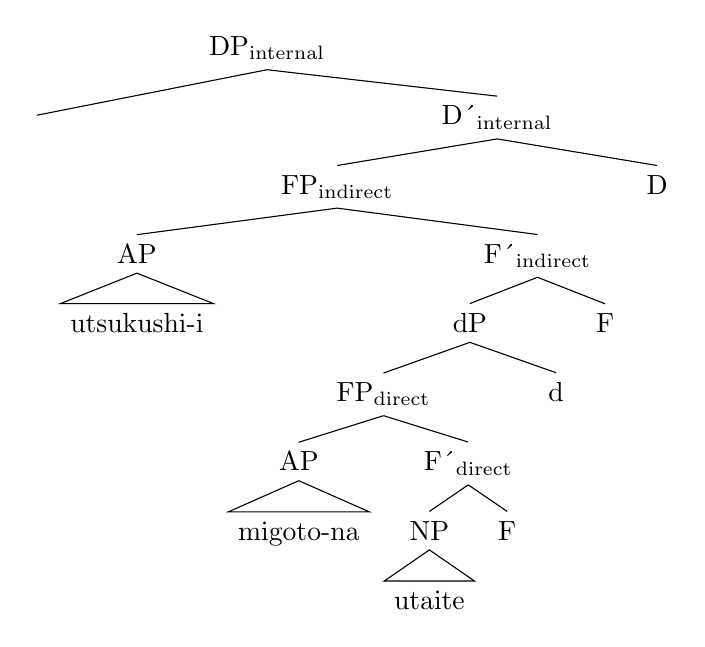
\begin{tikzpicture}[baseline=0pt, remember picture]
\tikzset{level distance=25pt, sibling distance=5pt}
\Tree [.DP\textsubscript{internal} {} [.D´\textsubscript{internal} [.FP\textsubscript{indirect} [.AP \edge[roof]; utsukushi-i ] [.F´\textsubscript{indirect} [.dP [.FP\textsubscript{direct} [.AP \edge[roof]; migoto-na ] [.F´\textsubscript{direct} [.NP \edge[roof]; utaite ] F ] ] d ] F ] ] D ] ]
\end{tikzpicture}

The same structural positions are at stake in the following minimal pair. The non-intersective modifier \textit{shōrai-no} `future' must be closer to the noun than the \textit{na}-adjective \textit{majime-na} `hardworking'. Again, an indirect, or at least ambiguous, modifier must precede the direct-only modifier showing its higher position within the DP. %\is{adjective ordering restrictions}

\ex. \ag. majime-na shōrai-no purosakkāsenshu\\
hardworking-\textsc{mod} future-\textsc{mod} football.player\\
`a hardworking person who will be a professional football player in the future’
\bg. ??shōrai-no majime-na purosakkāsenshu\\
future-\textsc{mod} hardworking-\textsc{mod} pro.football.player\\

Crucially, a hierarchy based on intersectivity can hardly be established in Japanese and rather all these examples seem rather to involve a direct/indirect dichotomy. Recall from Chapter \ref{japanesedp} that truly non-intersective modifiers also do not engage in ordering hierarchies with other types of direct modifiers, for example the equivalents of relational adjectives, to be reviewed below. This is exemplified in \ref{tada} with the non-intersective modifier \textit{tada-no} `mere’. \ref{tadada} shows that this modifier cannot occur predicatively.\footnote{Only with the meaning `mere’ is it never possible in predicative position. \textit{Tada-no} can also have the meaning `for free’, in which case it can be used predicatively. Therefore it is sorted in group 1 in the data set.} %\is{scope}

%\newpage

\ex. \label{tada} non-intersective vs. relational modifier
\ag. tada-no Doitsu-no gakusei\\
mere-\textsc{mod} German-\textsc{mod} student \label{tada1}\\
\bg. Doitsu-no tada-no gakusei\\
German-\textsc{mod} mere-\textsc{mod} student\\
`a mere German student' \label{tada2}

\exg. *Kono gakusei-wa tada-da.\\
this student-\textsc{top} mere-\textsc{cop}\\
(`This student is mere.’) \label{tadada}

This discussion has shown that non-intersective modifiers do exist in Japanese and that they predominantly can be found in the group of \textit{no}-modifiers. Furthermore, it was shown that the well-known ambiguous cases in English are resolved in Japanese, which is a substantial problem for \citet{baker:2003:verbal} who correlates the apparent lack of non-intersectivity with a lack of direct modification. Finally, since non-intersective modifiers are direct, they are merged lower than indirect modifiers and appear closer to the noun, explaining the mismatches between the assumptions of \citet{svenonius:2008:position} and \citet{ayano:2010:revisiting}.

\subsection{Relational modifiers}
\label{RAJapanese}

The second cross-linguistic group of direct-only modifiers are \textit{relational adjectives}, although in Japanese it might be better to speak of \textit{relational modifiers}. Those modifiers were discussed in Chapter \ref{RA} with regard to European languages (cf. \citealt{fabregas:2007:internal, rainer:2013:can, bortolotto:2016:RA}). %\is{relational modifiers}

Japanese, besides Arabic, was one of the two Non-European languages looked at to verify this category cross-linguistically in \citet{bisetto:2010:RA}, which explains the surprising amount of literature on this category with regard to Japanese \citep{nagano:2015:RA, nagano:2016:are, nagano:2018:conversion, shimada:2018:relational, morita:2010:internal, morita:2011:three, morita:2013:morph}. \citet{bisetto:2010:RA}, highlighting derivational factors, analyzes the suffix -\textsc{teki} 的 `-ic' as the derivational suffix of relational adjectives in Japanese.\footnote{Examples include \textit{keizai-teki} `economical' derived from \textit{keizai} `economy' or \textit{shukan-teki} `subjective' derived from \textit{shukan} `subjectivity’, cf. also \citet[71–73]{bisetto:2010:RA}.} However, as shown in \citet[48–50]{nagano:2016:are}, these derivates are not true equivalents of relational adjectives, since they in fact can be used predicatively and are gradable. Rather, the equivalents of relational adjectives appear in Japanese unequivocally with the element \textsc{no} and are not subject to morphological processes. Those equivalents seem to be nominal not only on the deep, but also on the surface level.

In the following, I will first show that the equivalents of \textit{thematic} and \textit{classificatory} relational adjectives exist in Japanese and then give an overview of the categories named in \citet{nagano:2016:are}, discussing some of them in sufficient detail in order to show which are candidates for direct modifiers, and where deviations might occur.

\subsubsection{Thematic and classificatory relational modifiers}

In Chapter \ref{RA}, it was outlined that relational adjectives in European languages come in two types: \textit{classificatory} and \textit{thematic}. Only the equivalents of classificatory relational adjectives are discussed in the literature with regard to Japanese. An example is given below. Observe that, contrary to the English equivalent \textit{environmental crisis}, no derivational processes are observable on the morphological level. %\is{relational modifiers}

\exg. kankyō-no kiki \\
environment-\textsc{mod} crisis\\
`environmental crisis’

As observable above, the equivalents of the classificatory adjective \textit{environmental} is a \textit{no}-modifier which expresses a certain relationship to the noun it modifies. Crucially however, \textit{kankyō} is a noun itself. Besides the absence of morphological derivation, this can also be exemplified on the syntactic level via productive use with case particles. %\is{relational modifiers}

\exg. Kankyō-ga daiji-da.\\
environment-\textsc{nom} important-\textsc{cop}\\
`The environment is important.’

As far as competing constructions go, \textit{of}-phrases (\textit{problems of the economy}) or PPs are not available, yet Japanese makes frequent use of lexical compounds, often Sino-Japanese four character lexical compounds, with the same meaning.

\exg. kankyō-kiki (環境危機)\\
environment-crisis\\
`environmental crisis’

Thematic relational adjectives have not been identified as a separate type of relational modifiers with regard to Japanese, probably because such modifiers are nominals in the first place. Recall that thematic relational adjectives are, in languages such as English, restricted to the modification of event or action nouns \citep{grimshaw:1991:argument}. A direct equivalent of such examples would be \ref{machi hatten} in which \textit{machi-no} `urban’ could be interpreted as a \textit{thematic relational modifier} since it expresses a subject role. %\is{thematic modifiers}

\exg. machi-no hatten\\
city-\textsc{mod} development\\
`urban development / development of the city’ \label{machi hatten}

Event nouns in Japanese usually belong to the category of so-called \textit{Verbal Nouns} \citep{teramura:1982:nihongo, oshima:2019:gradability}. Such nouns can either appear as true nouns, as in \ref{machi hatten}, or as predicates of a clause together with the light verb \textit{su} `to do’. \ref{machi-ga hatten} is a paraphrase of \ref{machi hatten}, in which \textit{hatten} serves as the predicate of the matrix clause and \textit{machi} now appears as a noun with the nominative case particle. %\is{verbal nouns}

\exg. Machi-ga hatten-shi-ta.\\
city-\textsc{nom} development-do-\textsc{pst}\\
`The city developed.’ \label{machi-ga hatten}

Since such modifiers appear very nominal, no special discussion on their character seems necessary at first. Nevertheless, in Japanese, neither the equivalents of classificatory \ref{kiki}, nor of thematic relational adjectives \ref{machi} can serve as the predicate of a sentence together with the copula.

\newpage

\ex. \ag. *Kiki-ga kankyō-da.\\
crisis-\textsc{nom} environment-\textsc{cop}\\
(`The crisis is environmental.’) \label{kiki}
\bg. *Hatten-ga machi-da.\\
development-\textsc{nom} city-\textsc{cop}\\
(`The development is urban.’) \label{machi}

\subsubsection{Different categories}

A further obstacle for the precise analysis of relational modifiers in Japanese is the abundance of possible categories scattered in the literature, for which it is not clear if all really fulfill the relevant syntactic criteria. A very detailed list of categories is presented in \citet[53–54]{nagano:2016:are}, who understands relational adjectives in Japanese as non-predicative modifiers with a nominal character. In the table below, I give her categories and compare them to the categories presented in hierarchies of relational adjectives written in the cartographic research field \citep{rae:2010:ordering, bortolotto:2016:RA}, to older approaches to relational adjectives in English (\citealt{downing:1977:creation, levi:1978:syntax, warren:1984:classifying}), to standard hierarchies of qualitative adjectives, and to the PP hierarchy of \citet{takamine:2010:hierarchy}.\footnote{This table is most of all meant to serve as a reference. See also \citet[93–94]{bortolotto:2016:RA} as well as \citet[16]{rainer:2013:can} for similar comparisons.} %\is{relational modifiers}

\begin{center}
\begin{longtable}{|c|p{8cm}|p{3cm}|}
\hline
\textbf{Nagano (2016)} & \textbf{In other hierarchies} & \textbf{Example} \\
\hline
\endfirsthead
\multicolumn{3}{c}
{\tablename\ \thetable\ -- \textit{Continued from previous page}} \\
\hline
\textbf{Nagano (2016)} & \textbf{In other hierarchies} & \textbf{Example}\\
\hline
\endhead
\hline
\multicolumn{3}{c}{\textit{Continued on next page}} \\
\endfoot
\hline
\caption{Categories of Japanese Relational Modifiers compared to other studies}\\
\endlastfoot
\hline
Material & \citep{scott:2002:stacked, laenzlinger:2005:french, laenzlinger:2011:elements}: \textit{Material} (QA) & \textit{komugi-no pan}\\
& \citet{rae:2010:ordering, bortolotto:2016:RA}: \textit{Material} (RA) & `wheat(-en) bread' \\
& \citet{takamine:2010:hierarchy}: \textit{Material} (PPs) & \\
\hline
Nationality & \citet{sproat:1991:the}: \textit{Provenance} (QA) & \textit{Chūgoku-no kabin} \\
& \citet{scott:2002:stacked, cinque:2010:adj, laenzlinger:2005:french, laenzlinger:2011:elements}: \textit{Nationality/Origin} (QA) & `Chinese vase' \\
& \citet{alex:2011:ea, arseni:2014:EA}: \textit{Ethnic Adjectives} & \\
\hline
Shape & \citet{sproat:1991:the}: \textit{Shape} (QA) & \textit{sankaku-no heya}\\
& \citet{scott:2002:stacked, cinque:2010:adj, laenzlinger:2005:french, laenzlinger:2011:elements}: \textit{Shape}(QA) & `triangular room'\\
\hline
Style/Pattern & no direct equivalent & \textit{shima-no uwagi} `striped jacket' \\
\hline
Type & potentially \citet{downing:1977:creation}: \textit{comparison} (RA) & \textit{Yōroppa-no keizai} \\
& potentially \citet{warren:1984:classifying}: \textit{comparant-compared} (RA) & `European economy' (= European type of economy) \\
\hline
Tendency towards & no direct equivalent & \textit{ame-no kisetsu} `rainy season' \\
\hline
Line/Family/Group & close to \textit{group adjectives} \citep{grimshaw:1991:argument, cetnarowska:2015:categorial} & \textit{Surabu-no gengo} `Slavic languages' \\
\hline
Location & \citet{downing:1977:creation}: \textit{place} (RA) & \textit{umi-no seibutsu}\\
& Levi (1978): \textit{in} (RA) & `marine life'\\
& \citet{warren:1984:classifying}: \textit{place-object} (RA) & \\
& \citet{rae:2010:ordering, bortolotto:2016:RA}: \textit{Location} (RA) & \\
& \citet{takamine:2010:hierarchy}: \textit{Location} (PPs) & \\
\hline
Time & \citet{downing:1977:creation}: \textit{time} (RA) & \textit{yoru-no hōmon}\\
& \citet{levi:1978:syntax}: \textit{in} (RA) & `nocturnal visit'\\
& \citet{warren:1984:classifying}: \textit{time-object} (RA) & \\
& \citet{rae:2010:ordering, bortolotto:2016:RA}: \textit{Time} (RA) & \\
& \citet{takamine:2010:hierarchy}: \textit{Time} (PPs) & \\
\hline
Topic & \citet{levi:1978:syntax}: \textit{about} (RA) & \textit{keitai-no mondai}\\
& \citet{rae:2010:ordering, bortolotto:2016:RA}: \textit{Matter} (RA) & `morphological problem(s)' \\
\hline
Status & \citet{downing:1977:creation}: \textit{occupation} (RA) & \textit{fuku-daitōryō-no ninki} `vice-presidential term'\\
& \citet{warren:1984:classifying}: \textit{affected object-actor} (RA) & \\
& included in \textit{group adjectives} (\citealt{grimshaw:1991:argument, cetnarowska:2015:categorial}) & \\
\hline
Possession & potentially \textit{part-whole} in Warren (1984) & \textit{yotsu-ashi-no dōbutsu} `four-legged animal'\\
& \citet{nikolaeva:2012:possession, nikolaeva:2020:mixed, spencer:2017:denominal}: non-canonical modification carried out by nouns or relational adjectives & \\
\end{longtable}
\end{center}


It would take us too far afield to discuss each of these categories above. Instead, I will concentrate on a sample of relevant categories, most importantly \textsc{nationality}, \textsc{material} and \textsc{shape}. The reason for this is that these categories also appear in well-known hierarchies for \textit{qualitative} adjectives. It will be shown that modifiers of \textsc{nationality} and \textsc{material} have a strong direct character in Japanese. Modifiers of \textsc{shape}, on the other hand, do not. In the second part of this section, I will put forth data concerning combination with the different forms of the copula and discuss ordering and possible hierarchies.

\subsubsection{NATIONALITY and ethnic modifiers}

Modifiers of \textsc{nationality} are quite intriguing in Japanese. This category is quite low in ordering hierarchies of qualitative adjectives in the literature (cf. \citealt{scott:2002:stacked}). Recall, on the other hand, the group of \textit{ethnic adjectives}, which has been put forth for various languages as toponymic relational adjectives denoting an origin (\citealt{bartning:1984:aspects, bosque:1996:postnominal, gunkel:2008:constraints, alex:2011:ea} a. o.). It is unclear whether the term \textit{ethnic adjectives} is applicable only with regard to thematic, or also to classificatory adjectives denoting an origin. Recall that the latter type can be used predicatively in English \ref{bedsheet}, while \textsc{nationality} adjectives with a thematic reading, those modifying event nouns, cannot \ref{attack} (cf. \citealt{alex:2011:ea}). %\is{ethnic modifiers}

\ex. \a. These bed sheets are Italian. \label{bedsheet}
\b. *This attack was Italian. \label{attack}

In the literature on Japanese, only equivalents of \textsc{nationality} modifiers with object nouns are given \citep{morita:2011:three, nagano:2016:are}, for example \ref{nihon-no kuruma}.\footnote{Note that in this example, the modifier \textit{Nihon-no} does not necessarily denote an origin, or nationality, but might denote several other relations to the head noun, including \textsc{location} on a reading `in Japan’.}

\exg. Nihon-no kuruma\\
Japan-\textsc{mod} car\\
`Japanese car' \label{nihon-no kuruma}

Similar to thematic relational modifiers, the equivalents of thematic ethnic adjectives have probably not been discussed due to the fact that they just seem to highlight a case of modification by a noun. Arguably, an example could be the following, given in passing by \citet[48]{nagano:2016:are}. %\is{ethnic modifiers}

\exg. Nihon-no kōgeki\\
Japan-\textsc{mod} attack\\
`Japanese attack'

It is a crucial observation that \textsc{nationality} modifiers in Japanese, also those with a classificatory meaning, are only used attributively, never predicatively \ref{kurumanihonda} and are non-gradable \ref{totemonihon}, \ref{yorinihon}. Importantly, gradability is not even possible with endpoint modifiers as shown in \ref{kanzenni}. This crucially differentiates them from English classificatory adjectives. %\is{ethnic modifiers}

%\newpage

\ex. \ag. Nihon-no kuruma\\
Japan-\textsc{mod} car\\
`Japanese car'
\bg. *Kono kuruma-wa Nihon-da.\\
this car-\textsc{top} Japan-\textsc{cop}\\
(`This car is Japanese.’) \label{kurumanihonda}
\cg. *totemo Nihon-no kuruma\\
very Japan-\textsc{mod} car\\
(`very Japanese car’) \label{totemonihon}
\dg. *Watashi-no kuruma-wa sensei-no kuruma-yori Nihon (no kuruma) da.\\
I-\textsc{mod} car-\textsc{top} teacher-\textsc{mod} car-than Japan \textsc{mod} car \textsc{cop}\\
(`My car is more Japanese than my teacher's (car).’) \label{yorinihon}
\eg. *kanzenni Nihon-no kuruma\\
completely Japan-\textsc{mod} car\\
(`completely Japanese car’) \label{kanzenni}

What holds for classificatory, also holds for the equivalents of thematic ethnic modifiers as shown below.

\newpage

\ex. \ag. Nihon-no kōgeki\\
Japan-\textsc{mod} attack\\
`Japanese attack'
\bg. *Kono kōgeki-wa Nihon-da.\\
this attack-\textsc{top} Japan-\textsc{cop}\\
(`This attack is Japanese.’)
\cg. *totemo / kanzenni Nihon-no kōgeki\\
very / completely Japan-\textsc{mod} attack\\
(`very / completely Japanese attack’)

While in English, \textsc{theme} readings of ethnic adjectives have been argued to be impossible \citep{kayne:1981:ecp, giorgi:1991:syntax},\footnote{Nevertheless such readings have been marginally reported in English \citep{arseni:2014:EA} and seem productive in Polish \citep{cetnarowska:2015:categorial}.

\par

\ex. the French defeat \null\hfill \citep[23]{arseni:2014:EA}

\exg. chiń-s-ka pora\v{z}ka (Polish)\\
China-\textsc{ra-nom.sg.f} destruction.\textsc{nom.sg.f}\\
`destruction of China' \null\hfill \citep[136]{cetnarowska:2015:categorial}

\par


\citet[20]{rainer:2013:can} mentions that online he found ``dozens of examples of the type \textit{the Russian invasion by Napoleon, the Afghan invasion by Russia, the Polish invasion by Germany, the Chinese invasion by Japan}, and the like, many of which apparently occur in authoritative documents“.} no such restrictions are applicable to the Japanese equivalents, presumably for the fact that they are simply nouns. %\is{ethnic modifiers} %\is{Polish}

Furthermore, object and subject roles can both be expressed inside the same sentence as in \ref{sub-ob} (cf. \citealt{murasugi:1991:noun}). In such cases, the first modifier is usually interpreted as the subject and the second, the one adjacent to the noun, as the object. As expected, Japanese exhibits a rather free behavior of word order here as well and the reverse interpretations are not impossible.\footnote{Many other thematic roles can be expressed within the DP, but for most, an additional postposition needs to appear before \textsc{mod}.} %\is{thematic modifiers}

\exg. Amerika-no Itaria-no hakai \label{sub-ob}\\
America-\textsc{mod} Italy-\textsc{mod} destruction\\
`destruction of Italy by America’ \\ \null \hfill \textit{Amerika}=subject, \textit{Itaria}=object

Finally, modifiers of \textsc{nationality} can modify human nouns as the following example given in \citet[91]{morita:2011:three} shows. Again, predicative use is impossible, and so is gradability.

\newpage

\ex. \ag. Nihon-no haiyū\\
Japan-\textsc{mod} actor\\
`Japanese actor'
\bg. *Kono haiyū-wa Nihon-da.\\
this actor-\textsc{top} Japan-\textsc{cop}\\
(`This actor is Japanese.’)
\cg. *totemo Nihon-no haiyū\\
very Japan-\textsc{mod} actor\\
(`very Japanese actor’)
\dg. *Kono haiyū-wa sono haiyū-yori Nihon-no haiyū da.\\
this actor-\textsc{top} that actor-than Japan-\textsc{mod} actor \textsc{cop}\\
(`This actor is more Japanese than that actor.’)
\eg. *kanzenni Nihon-no haiyū\\
completely Japan-\textsc{mod} actor\\
(`completely Japanese actor’)

This might be different for other languages. \citet{arseni:2014:EA} have argued that all ethnic modifiers have an underlying origin-reading which arguably permits predicative use, as in the following example in English.

\ex. Guillem is French. \hfill \citep[23]{arseni:2014:EA}

In German, as in Japanese, such examples are clearly marked as also mentioned in \citet{kotowski:2016:adj}. %\is{German}

%\newpage

\exg. ??Guillem ist französisch. (German)\\
Guillem is French\\
`Guillem is French’

In order to express the nationality of a human entity in predicative position in Japanese, the suffix -\textit{jin} 人, lit. `human' needs to be added. Again, the same holds true in German \ref{franzose}.

\exg. Kono gekai-wa Nihon-*(jin)-da. (Japanese)\\
this surgeon-\textsc{top} Japan-person-\textsc{cop}\\
`This surgeon is Japanese.’ (= a Japanese person)

\exg. Guillem ist Franzose. (German)\\
Guillem is Frenchman\\
`Guillem is French’ (= a French person) \label{franzose}

A remaining question is how the thematic relation, the theta roles within DPs such as \ref{sub-ob} are being established. In the cartographic research literature, dedicated projections are given for modifiers that express a \textsc{theme} or \textsc{agent} reading \citep{cinque:1993:evidence, laenzlinger:2005:french, laenzlinger:2011:elements, bortolotto:2016:RA}. As for their derivation, \citet{laenzlinger:2011:elements} predicts that modifiers in the specifier positions of these projections have moved there from lower positions. Taking the parallel to the verbal domain seriously, nouns with a \textsc{theme} reading start out as complements of N, those with an \textsc{agent} reading as specifiers of an additional nP projection (see also \citealt{adger:2003:core}). One derivation could look as follows. Recall that the first modifier is typically interpreted as the agent, but that the reading can also be reversed, which underlines the unspecific nature of the functional projections within the direct domain. %\is{thematic modifiers}

%\newpage

\ex. \ag. Amerika-no\textsubscript{Agent} Itaria-no\textsubscript{Theme} hakai\\
America-\textsc{mod} Italy-\textsc{mod} destruction \null \hfill (= \ref{sub-ob})\\
\b. \begin{tikzpicture}[baseline=0pt, remember picture]
\tikzset{level distance=25pt, sibling distance=5pt}
\Tree [.DP\textsubscript{internal} {} [.D´ [.FP [.NP\textsubscript{1} \edge[roof]; {Amerika} ] [.F´ [.FP [.NP\textsubscript{2} \edge[roof]; {Itaria} ] [.F´ [.nP $<$NP\textsubscript{1}$>$ [.n´ [.NP {} [.N´ $<$NP\textsubscript{2}$>$ [.N hakai ] ] ] n ] ] F ] ] F ] ] D ] ]
\end{tikzpicture}

To summarize, modifiers of \textsc{nationality} are a productive source of direct modification in Japanese and the relevant lexemes clearly have a nominal status.

\subsubsection{Modifiers of MATERIAL}

\textsc{material} is in Japanese also exclusively expressed via \textit{no}-modifiers. These cannot be used predicatively \ref{komugida} and are not gradable \ref{totemokomugi}, as judged unequivocally so by all speakers I consulted in relevant constructions. One example is \textit{komugi-no} `wheat(-en)’, and recall also the examples with \textit{chīku-no} `teak’ from Chapter \ref{japanesedp}. %\is{material modifiers}

\newpage

\ex. \ag. komugi-no pan\\
wheat(-en)-\textsc{mod} bread\\
`wheaten bread'
\bg. *Kono pan-wa komugi-da.\\
this bread-\textsc{top} wheat(-en)-\textsc{cop}\\
(`This bread is wheat(-en).’) \label{komugida}
\cg. *totemo komugi-no pan\\
very wheat(-en)-\textsc{mod} bread\\
(`very wheaten bread’) \label{totemokomugi}

In contrast to modifiers of \textsc{nationality}, modifiers of \textsc{material} can be modified via endpoint modifiers \citep{kennedy:2005:scale, fabregas:2014:adjectival, oshima:2019:gradability} Cf. Chapters \ref{RA} and \ref{gradability}.

\exg. kanzenni komugi-no pan\\
completely wheat(-en)-\textsc{mod} bread\\
`completely wheaten bread’ (= bread consisting completely of wheat)

Finally, note that also modifiers of \textsc{material} are nominals and occur productively with case particles as shown below.

\exg. Ano komugi-wa oishi-i.\\
that wheat-\textsc{top} tasty-\textsc{cop}\\
`That wheat is tasty.’

Restrictions in predication and gradability are the reason why modifiers of \textsc{material} are closer to relational than to qualitative modifiers \citep{nagano:2016:are, morita:2011:three}. Their syntactic restrictions qualify them as direct modifiers.

\subsubsection{Modifiers of SHAPE are not direct-only}

The category \textsc{shape} is not a part of any study on relational adjectives in European languages, but is rather a central category of qualitative adjectives in \citet{sproat:1991:the, cinque:1993:evidence, cinque:2010:adj}, \citet{scott:2002:stacked} and \citet{laenzlinger:2005:french, laenzlinger:2011:elements}. Why is it treated then as a relational modifier in \citet{nagano:2016:are} and also \citet{morita:2010:internal, morita:2011:three}? First, note that the category \textsc{shape} is expressed in Japanese via \textit{i}- and \textit{na}-adjectives, but also via \textit{no}-modifiers and that there are lexemes, such as \textit{maru} `round' and \textit{shikaku} `square’, which can appear with either \textsc{i} or \textsc{no} in attributive position.\footnote{The BCCWJ yields 405 results with -\textsc{i} and 74 with -\textsc{no} for \textit{shikaku}, and even 33 with -\textsc{na}. It is a matter of debate whether we should predict to different spell-out forms of \textsc{mod} or simply two different lexemes which differ in word class status and thus lead to a different form of the syntactic head. The latter option seems more attractive in the system presented here, but, at the moment, nothing hinges on this.} %\is{shape modifiers}

%\newpage

\ex. \ag. maru-i / maru-no tēburu\\
round-\textsc{mod} / round-\textsc{mod} table\\
`round table'
\bg. shikaku-i / shikaku-no heya\\
square-\textsc{mod} / square-\textsc{mod} room\\
'square room'

The authors predict that both gradability and predicativity are marked for the \textit{no}-variant of these lexemes, making them essentially equivalents of true relational adjectives. However, not only are there examples of predicative use in the corpus,\footnote{12 occurrences for \textit{shikaku-da}, which is still very little making it a prototypical direct modifier, but 88 for \textit{maru-da}.} predicative use is also accepted by many speakers, including the ones I asked, as shown below.

\ex. \ag. Kono heya-wa shikaku-da.\\
this room-\textsc{top} square-\textsc{cop}\\
`This room is square.’
\bg. Kono tēburu-wa maru-da.\\
this table-\textsc{top} round-\textsc{cop}\\
`This table is round.’

Regarding gradability, the \textit{no}-modifier-variant is marked in combination with the degree adverb \textit{totemo} `very’, compared to the \textit{i}-variant, showing that this is not for semantic reasons. None of my consultants accepted the combination of the degree adverb with \textit{maru-no} \ref{totemomaru}, and only two out of five judged \textit{totemo shikaku-no} `very square' to be marginally acceptable \ref{totemoshikaku}. %\is{shape modifiers} %\is{gradability}

\ex. \ag. *totemo maru-no tēburu\\
very round-\textsc{mod} table\\
`very round table' \label{totemomaru}
\bg. ??totemo shikaku-no heya\\
very square-\textsc{mod} room\\
`very square room' \label{totemoshikaku}

However, the following combinations involving gradability are perfectly fine.

\ex. \ag. motto shikaku-no heya\\
more square-\textsc{mod} room\\
`more square room’
\bg. omot-ta-yori maru-no tēburu\\
think-\textsc{pst}-than round-\textsc{mod} table\\
`a table (which is) rounder than X thought’

Indeed, there are some prototypical direct \textit{no}-modifiers in the data set that arguably express shape, such as \textit{hishigata-no} `diamond-shaped, rhombic' (37 attr., 4 pred.; cf. also \citealt[98]{morita:2011:three}) and \textit{yūkei-no} `tangible' (29 attr., 0 pred.), suggesting that direct \textsc{shape} modifiers do exist. However, importantly this is not the case for all modifiers of this category, unlike \textsc{nationality} or \textsc{material}. %\is{shape modifiers} %\is{gradability}

This discussion extends to modifiers of the category \textsc{color}: The four basic color terms \textit{aka} `red', \textit{ao} `blue', \textit{shiro} `white' and \textit{kuro} `black' can also appear with -\textsc{i} and -\textsc{no}, that is as adjectives or \textit{no}-modifiers.\footnote{A complementary distribution pointed out in the literature \citep{sawada:1992:meishi, kishita:2005:shikisai} is that the \textit{no}-variant, the color noun \citep{okami:2012:two, okami:2016:on}, serves the purpose of identification and must receive a ``contrastive interpretation" \citep{koopman:2016:further} thus is infelicitous in contexts where the referent does not need to be identified.} Again, both versions are possible predicatively, contrary to what is argued in \citet{morita:2011:three}, but the \textit{no}-variant is only marginally gradable \ref{totemoshiro}.\footnote{Note that direct-only modifiers of \textsc{color} do appear in the data set to be discussed in Chapter \ref{QM}.} %\is{color modifiers} %\is{gradability}

\ex. \ag. shiro-i / shiro-no kōto\\
white-\textsc{mod} / white-\textsc{mod} coat\\
`white coat' \null \hfill \citep{koopman:2016:further}
\bg. Kono kōto-wa shiro-da.\\
this coat-\textsc{top} white-\textsc{cop}\\
`This coat is white.’
\cg. *totemo shiro-no kōto\\
very white-\textsc{mod} coat\\
(`very white coat’) \label{totemoshiro}

\subsubsection{Other copula forms}

As outlined above, the absence of predicative use correlates with the impossible co-occurrence with other copula forms, including \textsc{de} used for coordination. This seems to be borne out for non-predicative relational modifiers in Japanese as exemplified below. Crucially, as noted in Chapter \ref{coordination copula}, these modifiers can neither appear as the second conjunct in coordinative structures \ref{kirei second}.\footnote{One apparent counterexample was the material modifier \textit{komugi} `wheat(-en)‘ where \textsc{de} could be understood as a postposition, denoting the material of origin so \textit{komugi-de kata-i pan} could have the interpretation `hard bread made from wheat'.} %\is{copula} %\is{coordination}

\exg. *Chūgoku-de kirei-na kabin\\
China-\textsc{pred} beautiful-\textsc{mod} vase\\
(`a Chinese and beautiful vase’)

\exg. *kirei-de Chūgoku-no kabin\\
beautiful-\textsc{pred} China-\textsc{mod} vase\\
(`a beautiful and Chinese vase’) \label{kirei second}

These data points highlight that \textsc{de} has to appear in phrasal contexts and always involves a predication structure (\citealt{bowers:1993:predication}, see Chapter \ref{copulaelements}). Even if only one modifier involved in the coordination structure does is banned from predication, coordination becomes ungrammatical.

Furthermore, as exemplified in \ref{komugi dearu}, in no instance was the canonical copula \textsc{de-ar-u} allowed in combination with non-predicative relational modifiers. This again speaks against analyses that treat \textsc{no} as some predicative element. %\is{copula}

\exg. *komugi-de-ar-u pan\\
wheat-\textsc{pred-cop-prs} bread\\
(`bread which is wheat(-en)’) \label{komugi dearu}

\subsubsection{Hierarchy and ordering of relational modifiers}

\citet{bortolotto:2016:RA} establishes an ordering hierarchy for relational modifiers based on Romance, given here in terms of structural selection. %\is{ordering restrictions}

\ex. \emph{Hierarchy of Relational Adjectives (based on \citealt[180]{bortolotto:2016:RA}})\\
\textsc{time} $>$ \textsc{location} $>$ \textsc{agent} $>$ \textsc{instrument} $>$ \textsc{matter} ($>$) \textsc{theme} $>$ N

Also recall that it is a characteristic of relational adjectives to be strictly adjacent to their head noun and not to allow permutation with qualitative adjectives, as shown below for English.

\ex. \a. big wooden table
\b. *wooden big table \null \hfill \citep[66]{bisetto:2010:RA}

In the DP structure presented in this book, no specific functional projections dedicated to the different categories of relational modifiers are included inside the direct domain. This predicts (correctly) that relational modifiers in Japanese are not ordered according to a specific hierarchy. However, \citet{watanabe:2012:direct} argues in favor of such a hierarchy. First, he mentions that modifiers of \textsc{nationality} and \textsc{material} have to be closer to their head noun than modifiers of other categories.\footnote{I give his judgments below, but it is not clear whether this is an issue of grammaticality or preference. Note also that he uses as contrast the non-predicative modifier \textit{chiisa-na} `small' (see Chapter \ref{rentaishi}).} %\is{relational modifiers}

%\newpage

\ex. \textsc{dimension} $\succ$ \textsc{material}
\label{chiisa1} \ag. chiisa-na ki-no hashi\\
small-\textsc{mod} wood-\textsc{mod} bridge\\
\bg. ??ki-no chiisa-na hashi\\
wood-\textsc{mod} small-\textsc{mod} bridge\\
`small wooden bridge' \hfill \citep[507]{watanabe:2012:direct}

\ex. \textsc{dimension} $\succ$ \textsc{nationality}
\label{chiisa2} \ag. chiisa-na Chūgoku-no kabin\\
small-\textsc{mod} China-\textsc{mod} vase\\
\bg. ??Chūgoku-no chiisa-na kabin\\
China-\textsc{mod} small-\textsc{mod} vase\\
`small Chinese vase' \hfill \citep[507]{watanabe:2012:direct}

Next, the author argues that the categories \textsc{nationality} and \textsc{material} reflect the structural hierarchy \textsc{nationality} $>$ \textsc{material} in linear order when occurring together.

%\newpage

\ex. \textsc{nationality} $\succ$ \textsc{material}
\label{hokuo} \ag. hokuō-no ki-no isu \\
North.Europe-\textsc{mod} wood-\textsc{mod} chair\\
\bg. *ki-no hokuō-no isu\\
wood-\textsc{mod} North.Europe-\textsc{mod} chair\\
`North European wooden chair' \hfill \citep[508]{watanabe:2012:direct}

\ex. \textsc{nationality} $\succ$ \textsc{material}
\label{Chiri} \ag. Chiri-no kin-no kubikazari\\
Chile-\textsc{mod} gold-\textsc{mod} necklace\\
\bg. *kin-no Chiri-no kubikazari\\
gold-\textsc{mod} Chile-\textsc{mod} necklace\\
`Chilean gold necklace' \hfill \citep[508]{watanabe:2012:direct}

However, first this assessment is not shared by all authors. \citet[Fn. 14]{nagano:2016:are} emphasizes that she does share the judgment for \ref{chiisa1} and also for \ref{hokuo}, but not for \ref{chiisa2} and \ref{Chiri}, meaning she does not have a preferred order. She suggests that the ordering restrictions in the other cases might be phonologically conditioned (ibid.). More precisely, speakers including Nagano might prefer a shorter modifier to the right of a longer one. This is the case for \textit{chiisa} `small' (3 morae) and \textit{hokuō} `North European' (4 morae) preceding \textit{ki} `wooden' (1 mora). It is not however for \textit{chiisa} `small' vs. \textit{Chūgoku} `China, Chinese' (3 vs. 4 morae) and \textit{Chiri} `Chile, Chilean' vs. \textit{kin} `gold(-en)' (both 2 morae). %\is{ordering restrictions} %\is{relational modifiers}

Furthermore, \textit{ki} `wooden’ is the only monomoraic modifier in the data set and might be the only one that triggers such ordering restrictions (cf. Chapter \ref{optionality}). Concerning \ref{Chiri}, Ken Hiraiwa (p.c.) mentioned to me that some speakers might think of \textit{kin-no kubikazari} `gold(-en) necklace' as a set phrase which is why separating the two entities is judged as not good.

I have tested for several ordering preferences among relational modifiers and in combinations with qualitative modifiers and could not detect any ordering restrictions. Importantly, in order to exclude the factors \textit{phonology} (the number of morae) and \textit{word class status} (\textit{i}-, \textit{na}-adjective, \textit{no}-modifier), I tried to verify ordering restrictions for different combinations and scenarios (see Chapter \ref{optionality}), however, in no case did I trigger an increase or decrease in preference for any speaker in any pair. In contrast, note the awkward English translation for almost all b) examples in the examples given below.

%\newpage

\ex. \textsc{nationality} vs. \textsc{material}
\ag. Denmāku-no chīku-no isu\\
Denmark-\textsc{mod} teak-\textsc{mod} chair\\
`Danish teak chair'
\bg. chīku-no Denmāku-no isu\\
teak-\textsc{mod} Denmark-\textsc{mod} chair\\
`teak Danish chair'

\ex. \textsc{quality} vs. \textsc{nationality}
\ag. kirei-na Chūgoku-no kabin\\
beautiful-\textsc{mod} China-\textsc{mod} vase\\
`beautiful Chinese vase'
\bg. Chūgoku-no kirei-na kabin\\
China-\textsc{mod} beautiful-\textsc{mod} vase\\
`Chinese beautiful vase'

\ex. \textsc{material} vs. \textsc{quality} (\textsc{shape})
\ag. komugi-no kata-i pan\\
wheat-\textsc{mod} hard-\textsc{mod} bread\\
`hard wheat(-en) bread'
\bg. kata-i komugi-no pan\\
hard-\textsc{mod} wheat-\textsc{mod} bread\\
`wheat(-en) hard bread'

\ex. \textsc{color} vs. \textsc{nationality}
\ag. ao-i Chūgoku-no kabin\\
blue-\textsc{mod} China-\textsc{mod} vase\\
`blue Chinese vase'
\bg. Chūgoku-no ao-i kabin\\
China-\textsc{mod} blue-\textsc{mod} vase\\
`Chinese blue vase'

Note also the following contrast given in \citet{nagano:2016:are}, which is identical to Watanabe’s example \ref{chiisa2} with the difference that the \textit{i}-adjective \textit{chiisa-i} `small’ is used instead of the \textit{rentaishi} \textit{chiisa-na} `small’.

\newpage

\ex. \textsc{dimension} vs. \textsc{nationality}
\ag. chiisa-i Chūgoku-no kabin\\
small-\textsc{mod} China-\textsc{mod} vase\\
`small Chinese vase'
\bg. Chūgoku-no chiisa-i kabin\\
China-\textsc{mod} small-\textsc{mod} vase\\
`Chinese small vase' \null \hfill \citep[57]{nagano:2016:are}

These facts emphasize that neither \textit{ordering restrictions} nor \textit{adjacency to the head noun} are valid criteria for the equivalents of relational modifiers in Japanese, which is expectable considering the broad direct domain of Japanese.

\subsubsection{Further issues: Nominal status and predicative use} \label{Ra japanese predicative}

There are two remaining issues concerning relational modifiers. First, since relational modifiers are rather nominal, they make up a prototype of direct nominals in Japanese as also mentioned in \citet{watanabe:2012:direct} for modifiers of \textsc{nationality} and \textsc{material}. This is shown below via productive combination with case particles \ref{chugoku kawatta} and the inability to be nominalized \ref{chugoku sa}. %\is{nationality modifiers}

\exg. Chūgoku-ga kawat-ta.\\
China-\textsc{nom} change-\textsc{pst}\\
`China has changed.’ \label{chugoku kawatta}

\exg. *Chūgoku-sa\\
China-ness \label{chugoku sa}\\

A further piece of evidence for nominal status is the fact that these modifiers can be modified themselves leading to bracketing ambiguities. As shown in \ref{katai komugi}, the \textit{i}-adjective \textit{kata-i} `hard’ can either modify \textit{pan} `bread’, skipping over \textit{komugi} `wheat(-en)’ which modifies \textit{pan} `bread’. On an alternative reading, \textit{kata-i} modifies \textit{komugi} `wheat(-en)’ yielding the DP \textit{kata-i komugi} `hard wheat’ which in turn modifies \textit{pan}.\footnote{Such bracketing ambiguities can be compared to cases of what \citet{nikolaeva:2020:mixed} call \textit{syntagmatic mixing}. In languages such as Selkup and other Samoyedic languages, relational adjectives, albeit being subject to derivational operations, can still be modified. In the Japanese case however, this seems closer to what \citet{spencer:2005:towards} calls \textit{indeterminacy}.} %\is{bracketing ambiguities}

\exg. kata-i komugi-no pan\\
hard-\textsc{mod} wheat-\textsc{mod} bread\\
1. $\approx$ `hard wheat(-en) bread’\\
2. $\approx$ `bread out of hard wheat' \label{katai komugi}

Another cross-linguistic phenomenon concerns predicative use. Recall that relational adjectives in various languages can be used predicatively, either as a result of a class shift to a qualitative adjective, or when they have a \textit{kind-reading} \citep{mcnally:2004:relational}. Another mechanism was noun ellipsis, facilitated in contrastive statements. In Japanese, as briefly mentioned in Chapter \ref{test predication}, relational modifiers also become possible in predicative position when they are connected to a certain kind of suffixes, referred to as \textit{bound markers} or \textit{relational nouns} in \citet{nagano:2016:are, shimada:2018:relational}. When these markers, which roughly correspond in their meaning to relational modifiers, are added to a relational modifier, a new entity called \textit{expanded modifiers} in \citet[54]{nagano:2016:are} is formed. These expanded modifiers are not only more specified in their meaning, they are also productive in predicative position. This is illustrated below where the pair \textit{chīzu} `cheese’ and \textit{iri} `put inside’ form \textit{chīzu-iri} `(with) cheese put inside’. As \citet{levi:1978:syntax} has argued for similar cases in English, establishing modifier and modified noun as a set facilitates predicative use. Interested readers are referred to Appendix A for an overview. %\is{bound markers}

\ex. \ag. chīzu-iri-no pan\\
cheese-put.in-\textsc{mod} bread\\
`bread with cheese put inside
\bg. kono pan-wa chīzu-*(iri)-da\\
this bread-\textsc{top} cheese-put.in-\textsc{cop} \\
`This bread is with cheese inside.’

Nouns to which the adjective-forming suffix -\textsc{teki} is added also become possible in predicative position and gradable. As mentioned at the beginning of this chapter, this suffix was argued originally by \citet{bisetto:2010:RA} to form relational adjectives in Japanese, but the examples below, illustrated with \textsc{nationality} adjectives with a \textsc{theme} reading, clearly show that a class shift to a qualitative adjective occurred (see also \citealt[48]{nagano:2016:are}).

\ex. \label{like} \ag. Ano kōgeki-wa America-*(teki)-d-at-ta.\\
this attack-\textsc{top} America-\textsc{adj}-\textsc{cop-pred-pst}\\
`This attack was (typical) American.'
\bg. totemo America-*(teki)-na kōgeki\\
very America-\textsc{adj}-na attack\\
`very American (= typical for Americans) attack'

\subsubsection{Summary: Characteristics of relational modifiers in Japanese}

Taking all these facts into account, Japanese does exhibit a category that is equivalent to the cross-linguistic category of relational adjectives. Due to their unclear lexical status, they are referred to as \textit{relational modifiers}. They show the following characteristics:

\newpage

\ex. \a. They generally cannot be used predicatively.
\b. They are not gradable.
\c. They cannot be coordinated.
\d. They can be used as real nouns.
\e. However, they do not show the typical ordering restrictions and strict adjacency to the head noun associated with relational adjectives in other languages.

\subsection{Direct qualitative modifiers} \label{QM}

Those authors who denied the existence of direct modification in Japanese \citep{sproat:1991:the, laenzlinger:2011:elements} only investigated modifiers of categories such as \textsc{dimension}, \textsc{shape} and \textsc{quality}, those categories which are related to \textit{qualitative} modification in European languages, where \textit{qualitative} is used contra \textit{relational}. In a sense, those categories form the most basic adjectival categories. The fact that no direct modifiers seem to be available for these categories in Japanese was thus directly related to the alleged absence of direct modification. Importantly, as also mentioned in the introduction, most modifiers of these categories are not direct-only in other languages either, and the status of a certain qualitative adjective in English does only become obvious in contexts of ordering \citep{cinque:2010:adj, laenzlinger:2011:elements}. %\is{direct qualitative modifiers}

However, Japanese exhibits several lexemes that one could classify as direct-only qualitative modifiers and these cases are worth discussing.\footnote{I have annotated (some) modifiers for their semantic category, but, of course, this is sometimes quite subjective. In any case, since the relevant functional projections are not active in Japanese, the semantic category of a modifier is not crucial.} Some potentially direct modifiers denoting \textsc{shape} were discussed above (\textit{hishigata-no} `diamond-shaped, rhombic’; \textit{yūkei-no} `tangible’). Examples of direct modifiers of the category \textsc{dimension} are the lexemes \textit{ōki} `big' and \textit{chiisa} `small’. Those can appear either with \textsc{i} or with \textsc{na}, without a substantial change in meaning. However, they never appear with the copula \textsc{da} \ref{ieokida}, only the \textit{i}-variant can be used predicatively. %\is{rentaishi}

\newpage

\ex. \ag. ōki-i / chiisa-i ie\\
big-\textsc{mod} / small-\textsc{mod} house\\
`big / small house'
\bg. Kono ie-wa ōki-i / chiisa-i.\\
this house-\textsc{top} big-\textsc{cop} / small-\textsc{cop}\\
`This house is big / small.’
\cg. ōki-na / chiisa-na ie\\
big-\textsc{mod} / small-\textsc{mod} house\\
`big / small house'
\dg. *Kono ie-wa ōki-da / chiisa-da.\\
this house-\textsc{top} big-\textsc{cop} / small-\textsc{cop}\\
(`This house is big / small.’) \label{ieokida}

There is also no use as adverbials or inchoatives attested for the \textit{na}-version of these lexemes, contrary to the corresponding \textit{i}-adjective, where \textsc{i} inflects to \textsc{ku}. %\is{rentaishi}

\exg. Ōki-\textbf{ku} / *ōki-\textbf{ni} nat-ta.\\
big-\textsc{adv} / big-\textsc{adv} become-\textsc{pst}\\
`Became big.’

Therefore, the \textit{na}-variants of these lexemes are also classified as \textit{rentaishi}, the topic of Chapter \ref{rentaishi}. An additional factor to discuss is that they are in fact gradable as illustrated below. Remember, however, that non-gradability is an accompanying factor of non-predicative modifiers, not a prerequisite \citep[47]{cinque:2010:adj}. %\is{direct qualitative modifiers}

\exg. Ichi-ban ōki-na no-wo eran-da.\\
number-one big-\textsc{mod} \textsc{ln}-\textsc{acc} choose-\textsc{pst}\\
`X chose the biggest one.’ \hfill \citep[1: 28]{sekine:1937:fukutaishi}

Potential other direct modifiers of \textsc{dimension} are documented in the data set, for instance \textit{ōgata-no} `large-scale' (709 attr., 73 pred.) and \textit{atsude-no} `thick’ (189 attr., 2 pred.). However, both are, in principle, possible in predicative position, albeit only marginally attested. This holds especially for \textit{atsude-no} whose possibility in predicative position was corroborated by some speakers despite its very few occurences. %\is{dimension modifiers}

Clearer cases of direct modifiers are found among the category \textsc{quality}, which is \textit{per se} one of the more, perhaps the most, versatile category. For instance, \textit{gokujō-no} `of highest quality' (142 attr. 5 pred.) or \textit{seirai-no} `innate’ (92 attr., 0 pred.) yield few to none predicative occurences.

Direct modifiers of the category \textsc{color} are \textit{shikkoku-no} `pitch black' (165 attr., 2 pred.) and \textit{konpeki-no} `deep blue’ (46 attr., 0 pred.). %\is{direct qualitative modifiers}

It is interesting to note that direct modifiers of some less canonical categories given in the very fine-grained hierarchy of \citet[106, 114]{scott:2002:stacked}, can be found as well. Examples include \textit{gokkan-no} `freezing cold’ (44 attr., 5 pred.) representing the category \textsc{temparature} or \textit{kyūsoku-na} `fast, rapid’ (599 attr., 4 pred.) for the category \textsc{speed}, illustrated below for \textit{gokkan-no}.

%\newpage

\ex. \ag. gokkan-no kisetsu\\
freezing.cold-\textsc{mod} season\\
`freezing cold season'
\bg. ??Ima-no kisetsu-wa gokkan-da\\
now-\textsc{mod} season-\textsc{top} freezing.cold-\textsc{cop}\\
`The season at the moment is freezing cold.’

Finally, there are some direct-only modifiers that do not fit any semantic category present in established hierarchies, such as \textit{kidai-no} `rare’ (71 attr., 0 pred.) and \textit{kaishin-no} `spot-on; critical’ (58 attr., 0 pred.).

\ex. \ag. kaishin-no ronbun\\
spot.on-\textsc{mod} essay\\
`a spot-on paper; a paper written to one's full satisfaction'
\bg. *Kono ronbun-wa kaishin-da.\\
this paper-\textsc{top} spot.on-\textsc{cop}\\
(`This paper is spot-on.’)

\ex. \ag. kidai-no sainō\\
rare-\textsc{mod} talent\\
`rare talent’ \label{kidai}
\bg. *Kare-no sainō-wa kidai-da.\\
he-\textsc{mod} talent-\textsc{top} rare-\textsc{cop}\\
(`His talent is rare.’)

Since the functional projections inside the direct domain are not governed by semantic categories, the problem in which functional projections to sort these modifiers disappears. They are merged in the direct domain, but in an unspecific functional projection.

%\newpage

\ex. \ag. kidai-no sainō\\
rare-\textsc{mod} talent\\
`rare talent’ (= \ref{kidai})
\b. 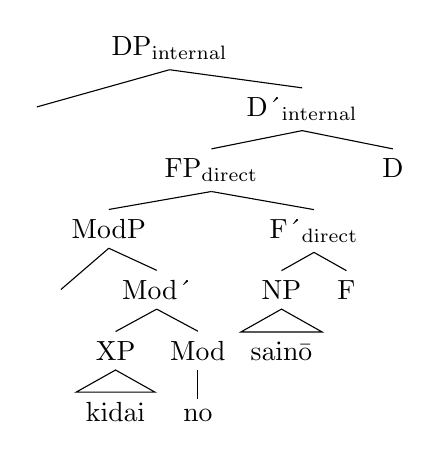
\begin{tikzpicture}[baseline=0pt, remember picture]
\tikzset{level distance=22pt}
 \Tree [.DP\textsubscript{internal} {} [.D´\textsubscript{internal} [.FP\textsubscript{direct} [.ModP {} [.Mod´ [.XP \edge[roof]; kidai ] [.Mod no ] ]] [.F´\textsubscript{direct} [.NP \edge[roof]; sainō ] F ] ] D ] ]
\end{tikzpicture}

\subsection{Idiomatic expressions} \label{idiomatic}

Another source for direct modification are modifiers involved in idiomatic expressions, although it might be better to speak of \textit{modifiers in non-free phrases}.\footnote{See \citet{melcuk:2012:phraseology, kohlich:2024:nonfree} for the difference between idiomatic expressions and collocations.} Recall that in English, only prenominal adjectives can elicit an idiomatic reading with their corresponding head noun, as for example \textit{white} in \textit{white lie} \citep[87–88]{cinque:2010:adj}. The only idiomatic expression with a single modifier given in the literature is as follows, given in \citet[122]{nagano:2015:RA}. As expected, predicative use is impossible with the idiomatic meaning. %\is{idiomatic modifiers}

\ex. \ag. aka-no tan'in\\
red-\textsc{mod} stranger\\
`a total stranger' (Lit. `a red stranger')
\bg. *Kono tan'in-wa aka-da\\
this stranger-\textsc{top} red-\textsc{cop}\\
only meaning: `This stranger is red.’

Several more idiomatic modifiers in Japanese can be identified, where ``idiomatic“ refers to modifiers that only co-occur with a certain noun, or a certain group of nouns with similar meaning. Thus, it is no prerequisite that a new meaning is formed, as in the example \textit{white lie}. One example of an idiomatic modifier, already mentioned in Chapter \ref{japanesedp}, is \textit{kōki-no} `curious’. This lexeme yields 69 results in attributive position, against zero with the copula. 61 out of those 69 occurrences are with nouns with the meaning `gaze, look’, among them \textit{me} (also `eye'), \textit{manazashi} `gaze' and \textit{shisen} `gaze, look'. The restriction in predicativity, and also gradability, is shown below.\footnote{Compared to \textit{me}, \textit{manazashi} and \textit{shisen} can be described as Sino-Japanese nouns with the same meaning from a higher register. Ken Hiraiwa has told me that to his native speaker ears the modification of \textit{manazashi} `gaze' via \textit{kōki-no} `curious’ seems to be truly idiomatic.} %\is{idiomatic modifiers}

\newpage
\ex. \ag. Shikashi kare-ga kōki-no me-de mi-rare, ōku-no hito-ga kare-no hanashi-wo kiki-ta-gat-ta koto[...]\\
but he-\textsc{nom} curious-\textsc{mod} eye-\textsc{ins} see-\textsc{pass} many-\textsc{mod} people-\textsc{nom} he-\textsc{mod} story-\textsc{acc} hear-\textsc{vol}-seem-\textsc{pst} fact\\
`But the fact that he was viewed with curious eyes (a curious gaze) and many people wanted to hear his story [...]’\footnote{Ogawa, Ryō (2002): Doreishōnin Soniē - 18-seiki Furansu no doreikōki to Afurika-shakai, Tokyo: Yamakawa Shuppansha, via BCCWJ, 2023/11/09.}
\bg. *Kare-ga mi-rare-ta me-wa kōki-dat-ta.\\
he-\textsc{nom} see-\textsc{pass-pst} eye-\textsc{top} curious-\textsc{cop-pst}\\
(`The eye/gaze he was viewed with was curious.’)
\cg. *totemo kōki-no me\\
very curious-\textsc{mod} eye\\
(`very curious gaze’)

Other examples include the modifiers \textit{higō-no} `unnatural’ (47 attr., 0 pred.) which occurs only with \textit{shi} `death’ and \textit{saigo} `end’ (also in the sense of `death’) \ref{higo-no} and \textit{anmoku-no} `tacit’ (350 attr., 0 pred.), mostly with \textit{ryōkai} `agreement’.\footnote{Two things are noteworthy here: First, the combination of \textit{higō} `unnatural’ and the two nouns are in 32 out of 47 cases part of the larger expression \textit{higō-no shi/saigo-wo toge-ru} `to meet an unnatural death’. Second, the modifier \textit{anmoku-no} `tacit’ does not yield a single instance of predicative use in the BCCWJ-corpus, but some instances can be found on Google. Nevertheless, it is also given in the literature \citep{muraki:2012:nihongo, lehmann:2015:japanisch} as a non-predicative modifier.} %\is{idiomatic modifiers}

\ex. \label{higo-no} \ag. Nanninka-no Kirisuto-kyōtō-wa higō-no shi-wo toge-ta.\\
several.people-\textsc{mod} Christianity-believer-\textsc{top} unnatural-\textsc{mod} death-\textsc{acc} meet-\textsc{pst}\\
`Several Christians met an unnatural death.’\footnote{Ōno, Kazumichi (2001): Translation of Michelet, Jules: \textit{Bible de l’humanité}. Tokyo: Fujiwara shoten, original: 1864, via BCCWJ, 2023/11/09. Note that potentially, sticking to the religious dimension of the modifier, a translation along the line of `undignified’ might be more appropriate.}
\bg. *Nanninka-no Kirisuto-kyōtō-ga toge-ta shi-wa higō-d-at-ta.\\
several.people-\textsc{mod} Christianity-believer-\textsc{nom} meet-\textsc{pst} death-\textsc{top} unnatural-\textsc{pred-cop-pst}\\
(`The death several Christians met was unnatural.’)

These data points suggest three things: First, idiomatic expressions do exist in Japanese. Second, they seem to offer another source for direct modification. Third, they are mostly found in the domain of \textit{no}-modifiers.

As shown in Chapter \ref{japanesedp}, \citet{svenonius:2008:position} suggests that idiomatic modifiers are merged as specifiers of category-less root phrases $\sqrt{}$P, embedded under nP \citep{marantz:1997:no}. They, thus, modify the very core at the noun \citep[36–37]{svenonius:2008:position}. Hence, their position is the lowest inside the direct domain, and therefore within the whole DP.

Concrete evidence for this claim comes from the fact that nothing can intervene between the idiomatic modifier and the head noun, i.e. the idiomatic modifier cannot be higher in the structure. This is shown for English in \citet[36–37]{svenonius:2008:position}, and also holds in Japanese \ref{koki low}. %\is{idiomatic modifiers}

\ex. \label{koki low} \ag. minna-no kōki-no manazashi\\
everyone-\textsc{mod} curious-\textsc{mod} gaze\\
`everyone's curious gaze'
\bg. *kōki-no minna-no manazashi\\
curious-\textsc{mod} everyone-\textsc{mod} gaze\\

Crucially, this behavior is not due to \textit{minna-no} `everyone’s’. As shown below, this modifier can intervene between non-idiomatic modifiers and the head noun.

\ex. \ag. minna-no aka-i doresu\\
everyone-\textsc{mod} red-\textsc{mod} dress\\
\bg. aka-i minna-no doresu\\
red-\textsc{mod} everyone-\textsc{mod} dress\\
`everyone's red dresses'

The adjacency facts apply to other idiomatic modifiers as well, for example the combination \textit{aka-no tan'in} `red stranger', tested with an intervening relative clause.

%\newpage

\ex. \ag. [dare-mo shira-na-i] aka-no tan'in\\
everyone-\textsc{emp} know-\textsc{neg}-\textsc{mod} red-\textsc{mod} stranger\\
`the total stranger that no one knows'
\bg. *aka-no [dare-mo shira-na-i] tan'in\\
red-\textsc{mod} everyone-\textsc{emp} know-\textsc{neg-mod} stranger\\

This thus yields the following position for idiomatic modifiers repeated from Chapter \ref{japanesedp}, now including the internal structure of the idiomatic modifier under ModP.

\newpage

\ex. 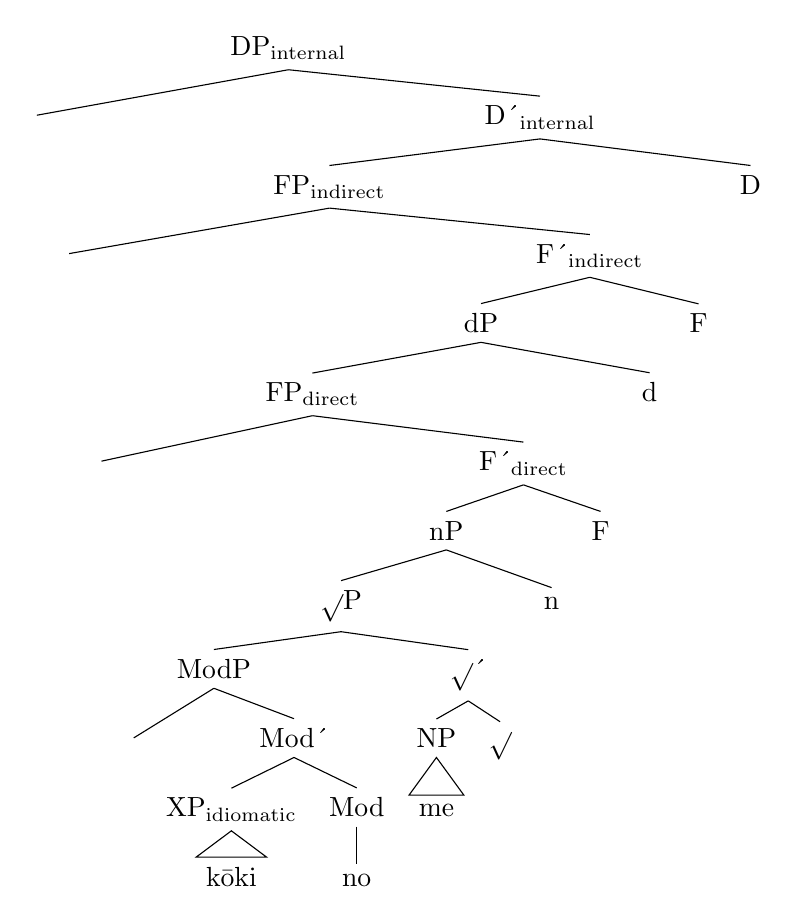
\begin{tikzpicture}[baseline=0pt, remember picture]
\tikzset{level distance=25pt, sibling distance=5pt}
\Tree [.DP\textsubscript{internal} {} [.D´\textsubscript{internal} [.FP\textsubscript{indirect} {} [.F´\textsubscript{indirect} [.dP [.FP\textsubscript{direct} {} [.F´\textsubscript{direct} [.nP [.$\sqrt{}$P [.ModP {} [.Mod´ [.XP\textsubscript{idiomatic} \edge[roof]; kōki ] [.Mod no ] ] ] [.$\sqrt{}$´ [.NP \edge[roof]; me ] $\sqrt{}$ ] ] n ] F ] ] d ] F ] ] D ] ]
 \end{tikzpicture}

Two more things are noteworthy. First, this root phrase \textit{only} hosts idiomatic modifiers in Japanese. \citet[130]{kim:2019:syntax}, who adopts the category $\sqrt{}$P from \citet{svenonius:2008:position}, argues that this phrase hosts idiomatic modifiers, but also modifiers which receive an internal theta role from the noun, thus compound-like constructions, in Korean. As evidence, she shows that no other modifier can intervene between such modifiers and the head noun in Korean either, parallel to idiomatic constructions. In the following example, \textit{kyengcey} `economy' is the internal argument of \textit{kayhyek} `renovation‘ and must be immediately adjacent to the noun \citep[130]{kim:2019:syntax}, reflecting essentially the category of relational modifiers discussed above. %\is{idiomatic modifiers} %\is{Korean}

%\newpage

\ex. \ag. sin kyengcey kayhyek (Korean)\\
new economy renovation\\
`a new renovation of the economy'
\bg. *kyengcey sin kayhyek\\
economy new renovation \null \hfill \citep[130]{kim:2019:syntax}\\

However, this is not the case in Japanese, as the translation of the examples shows. Here, permutation is easily possible.\footnote{This also extends to some examples given by \citet{laenzlinger:2011:elements}, such as \ref{machi-no saikin-no}. Here, a thematic modifier with a \textsc{theme} role (\textit{machi-no} `city’) and another modifier (\textit{saikin-no} `recent’), according to \citet{laenzlinger:2011:elements} have to appear in this order, thus showing the opposite pattern to Kim’s.

\par

\exg. machi-no saikin-no hakai\\
city-\textsc{mod} recent-\textsc{mod} destruction\\
`the recent destruction of the city’ \hfill \citep[227–228]{laenzlinger:2011:elements} \label{machi-no saikin-no}

\par


However, this DP is probably not very natural to begin with. Furthermore, without context, permutation is easily possible as well.}

\ex. \ag. arata-na keizai-no kaikaku\\
new-\textsc{mod} economy-\textsc{mod} renovation\\
\bg. keizai-no arata-na kaikaku\\
economy-\textsc{mod} new-\textsc{mod} renovation\\
`new renovation of the economy'

Second, \citet{okami:2012:two} has argued that those \textsc{color} modifiers which can appear with -\textsc{i} and -\textsc{no} can only receive an idiomatic reading in the \textit{i}-variant. She gives the following examples.

\ex. \ag. Tarō-to Hanako-wa aka-i / *aka-no ito-de musub-are-te-i-ru.\\
Taro-and Hanako-\textsc{top} red-\textsc{mod} / *red-\textsc{mod} string-\textsc{ins} bind-\textsc{pass-ger}-be-\textsc{prs}\\
`Taro and Hanako are destined to be together.’ (Lit. `bound by a red string’)
\bg. Kare-ni-wa kuro-i / *kuro-no uwasa-ga ar-u.\\
he-\textsc{dat-top} black-\textsc{mod} / *black-\textsc{mod} rumor-\textsc{nom} be-\textsc{prs}\\
`There are dark rumors about him.’ \hfill \citep[96]{okami:2012:two}

Interestingly, such color items do allow permutation when occurring with another modifier, as opposed to the examples above.

%\newpage

\ex. \ag. Kare-ni-wa hen-na kuro-i uwasa-ga ar-u.\\
he-\textsc{dat-top} strange-\textsc{mod} black-\textsc{mod} rumor-\textsc{nom} \textsc{cop-prs}\\
\bg. Kare-ni-wa kuro-i hen-na uwasa-ga ar-u.\\
he-\textsc{dat-top} black-\textsc{mod} strange-\textsc{mod} rumor-\textsc{nom} \textsc{cop-prs}\\
`There are strange dark rumors about him.’

This might suggest that these are in fact not idiomatic modifiers, or at least they are not merged in the same position, the root phrase.

\subsection{Quantificational modifiers}

As already shown in Chapter \ref{quantificational modifiers}, another source for direct modifiers are quantifiers or more precisely quantificational modifiers. Many quantificational modifiers are direct-only, while some are only prototypically attributive. Examples of quantificational modifiers which cannot be used predicatively include \textit{kazukazu-no} `many’, \textit{amata-no} `a lot, many’ and \textit{shuju-no} `various’. %\is{quantificational modifiers}

\newpage

\ex. \ag. Kare-wa kazukazu-no shō-wo tot-ta.\\
he-\textsc{top} many-\textsc{mod} prize-\textsc{acc} take-\textsc{pst}\\
`He received many prizes.’
\bg. *Kare-ga tot-ta shō-wa kazukazu-desu.\\
he-\textsc{nom} take-\textsc{pst} prize-\textsc{top} many-\textsc{cop.pol}\\
(`The prizes he received were many.’)

\ex. \ag. Kare-wa shuju-no / amata-no shikaku-wo mot-te-i-ru.\\
he-\textsc{top} various-\textsc{mod} / many-\textsc{mod} qualification-\textsc{acc} have-\textsc{ger}-be-\textsc{prs}\\
`He has various / many qualifications.’
\bg. *Kare-ga mot-te-i-ru shikaku-wa shuju-desu / amata-desu.\\
he-\textsc{nom} have-\textsc{ger}-be-\textsc{prs} qualification-\textsc{top} various-\textsc{cop.pol} / many-\textsc{cop.pol}\\
(`The qualifications he has are various / many.’)

In Chapter \ref{quantificational modifiers}, it was argued that quantificational modifiers are merged first inside the direct domain, since they exhibit direct behavior, but can subsequently move to the left periphery, as they can precede not only demonstratives \ref{kazukazuano} but also other direct-only modifiers \ref{takusankomugi4}. Probably they do this to check off a [quantificational] feature. %\is{quantificational modifiers}

%\newpage

\ex. \ag. kazukazu-no ano mondai\\
many-\textsc{mod} that problem\\
`those many problems’ \label{kazukazuano}
\bg. takusan-no komugi-no pan\\
a.lot-\textsc{mod} wheat-\textsc{mod} bread\\
`many wheat(-en) (pieces of) bread’ \label{takusankomugi4}

\subsection{Rentaishi} \label{rentaishi}

Finally, I will discuss the controversial word class of \textit{rentaishi} 連体詞, also called \textit{fukutaishi} 副体詞, arguably a language-specific source for direct-only modifiers. This word class is comprised of several lexemes with different morphology, derived from other word classes and now fossilized so that they are only used as attributive modifiers. This is the reason why \textit{rentaishi} are typically named by many Japanese linguists working in more traditional frameworks as non-predicative lexemes whose only function is to modify nouns making them the only group of direct modifiers acknowledged in the literature for a long time (see the newer works mentioned throughout this chapter). %\is{rentaishi}

The word class \textit{rentaishi} makes up a controversial case, first, because it was created more upon historical and ideological than on syntactic grounds at the beginning of the 20th century, and second, since it is not accepted as an individual word class by all linguists, both in- and outside of Japan. This is also the reason why many linguists would probably not classify the lexemes presented in the following pages as direct-only modifiers, since they strongly resemble fixed expressions. Nevertheless, I will show that they are quite close to idiomatic, and sometimes also non-intersective, modifiers; and since the relevant lexemes only serve as attributive modifiers, they deserve a discussion here. I will give a brief introduction, and then discuss different subgroups. For more information the reader is referred to \citet{kohlich:2020:rentaishi, kohlich:2023:uninflecting}. %\is{rentaishi}

\subsubsection{Introduction: Terminology, diachrony, criteria, subgroups}

The term \textit{rentaishi} literally translates to \textit{adnominal-noun-word} and is in English usually translated as `adnoun’ or `prenoun’. German equivalents are \textit{Adnomen}, sometimes \textit{Adnominalie} \citep{rickmeyer:1995:japanische}. \textit{Rentaishi} were incorporated into the Japanese word class system at the beginning of the Meiji-Period (1868-1912). The important linguists of the time, especially MATSUSHITA Daizaburō (\citealt{matsushita:1976:kaisen}) and also \citealt{yamada:1908:nihon, mitsuya:1932:bunpo, sekine:1937:fukutaishi, kieda:1938:koto, tokieda:1941:kokugogaku, yuzawa:1979:kokugo})), realized that there are several lexemes in Japanese that are restricted to attributive use, do not inflect and whose sole function is to modify nouns. They also realized that such lexemes bear striking similarities to the \textit{defective} adjectives in Western (mostly Dutch and English) languages, which only inflect dependent on the noun they modify \citep{sugimoto:1967:kindai, sugimoto:1991:kokugo, kim:2006:kindai}. The new word class \textit{rentaishi} was created to incorporate all those defective lexemes, becoming an equivalent of the Western adjective. %\is{rentaishi}

Another important criterion of this word class is the morphological diversity of its members. Being fossilized derivates from other word classes and frozen in their morphological form and usage domain, explains not only the restriction to attributive position, it also predicts the absence of other inflectional forms. This is a major point of deviation from all major Japanese word classes which since the language reform of the Meiji-Period have been predominantly categorized on the basis of their shared morphological paradigms \citep{nitta:2000:bun}. %\is{rentaishi}

Starting with an example, there are several lexemes which look verbal on a morphological level -- because they are indeed derived from verbs -- but only appear as prenominal modifiers. In fact, all those verbal \textit{rentaishi} are derived from verbs fossilized in their attributive inflectional form (\textit{rentaikei}). They include verbal derivates ending in the simple non-past form such as \textit{aru} `(a) certain’ \ref{aru},\footnote{This \textit{aru} is homophonous to the existential/copular verb \textit{ar}- which is why some authors \citep{lehmann:2015:japanisch} treat these two elements as the same. However, the copula verb \textit{ar}- is generally incompatible with animate nouns, therefore it cannot be the same element as \textit{aru} in \ref{aru}.} derivates ending in the morpheme -\textsc{iu}, which signaled passive, potential or spontaneity, and itself inflected for attributive form, such as \textit{iwayuru} `so-called’ \ref{iwayuru}, and those ending in the past morpheme \textsc{ta}, such as \textit{taishita} `considerable’ \ref{taishita}. None of these modifiers can be used predicatively or is gradable, highlighting the role of \textit{rentaishi} for the present study. %\is{rentaishi}

\ex. \label{aru} \ag. aru gakusei\\
certain student\\
`a certain student'
\bg. *Gakusei-wa aru.\\
student-\textsc{top} certain\\
(`This student is a certain.’)
\cg. *motto / totemo aru gakusei\\
more / very certain student\\
(`a more / very certain student’)

%\newpage

\ex. \label{iwayuru} \ag. iwayuru gakusei\\
so-called student\\
`a so-called student'
\bg. *Kono gakusei-wa iwayuru.\\
this student-\textsc{top} so-called\\
(`This student is so-called.’)
\cg. *motto / totemo iwayuru gakusei\\
more / very so-called student\\
(`a more / very so-called student’)

\ex. \label{taishita} \ag. taishita sa\\
considerable difference\\
`a considerable difference’
\bg. *Sa-wa taishita.\\
difference-\textsc{top} considerable\\
(`The difference is considerable.’)
\cg. *motto / totemo taishita sa\\
more / very considerable difference\\
`more / very considerable difference’)

Other potential members of \textit{rentaishi} are derived from adjectives and appear in the attributive form of the premodern copula \textit{nari} or \textit{tari}.\footnote{\textit{tari} can be seen as an allomorph which was restricted to Sino-Japanese lexemes.} Again, the relevant lexemes in Modern Japanese are restricted to attributive use and are non-gradable.

\newpage

\ex. \ag. tannaru machigai\\
mere misunderstanding\\
`a mere misunderstanding'
\bg. *Machigai-wa tannaru\\
misunderstanding-\textsc{top} mere\\
(`The misunderstanding is mere.’)
\cg. * motto / totemo tannaru machigai\\
more / very mere misunderstanding\\
(`more / very mere misunderstanding’)

\ex. \ag. shutaru gen'in\\
main reason\\
`the main reason'
\bg. *Gen'in-wa shutaru.\\
reason-\textsc{top} main\\
(`The reason is main.’)
\cg. *motto / totemo shutaru gen'in\\
more / very main reason\\
(`more / very main reason’)

Recall the lexemes \textit{ōki} `big' and \textit{chiisa} `small’ which can either co-occur with \textsc{i} or with \textsc{na}, but never with the copula \textsc{da}. The \textit{na}-variant of these lexemes has traditionally also been called \textit{rentaishi}.\footnote{Another such case is \textit{okashi} `strange’. The question remains whether there is one stem with two possible attributive morphemes, or if the respective lexemes are derived from an \textit{i}-adjective-counterpart, have become fossilized and are now lexicalized as uninflectable \textit{rentaishi}. Both analyses are available (see also \citealt[Fn. 15]{oshima:2021:nihongo}), but I will assume that \textit{ōki-i} and its counterparts are \textit{i}-adjectives, whereas \textit{ōki-na} belong to a different word class. This conditions the spell-out of \textsc{mod}. See also Chapter \ref{complexdirect}.} %\is{rentaishi}

\exg. *Kono ie-wa ōki-da.\\
this house-\textsc{top} big-\textsc{cop}\\
(`This house is big.’) (= \ref{ieokida})

Finally, there are some lexemes that are counted as \textit{rentaishi} which end in \textsc{ga}, namely \textit{waga} `my/our' and \textit{onoga} `my’, and some that end in \textsc{no} such as \textit{honno} `only, mere’.\footnote{Now the nominative case particle, \textsc{ga} is the archaic genitive marker, accounting for the archaic flavor of DPs in which the relevant \textit{rentaishi} appear.}

In this sense, it is debatable, whether one should analyze \textit{honno} as a fossilized lexeme, with /no/ being part of the stem, or whether one should maintain the analysis presented here of /no/ as a syntactic head. An argument for the former is that the first result for \textit{honno} on the Corpus of Historical Japanese (CHJ) dates back to the year 900. Maintaining an analysis of \textit{rentaishi} as a closed class of historical lexemes, I tentatively opt for this analysis, although nothing immediately hinges on this. Note however, that this also means that not every direct-only \textit{no}-modifier (sorted in group 5) in the data set is a \textit{rentaishi}, and \textit{rentaishi} is here not treated as a feature, but as a word class of historical derivates, despite recent efforts of several authors to argue for exactly that \citep{muraki:1996:imi, muraki:2009:nihongo, muraki:2012:nihongo, muraki:2015:hinshi, oshima:2021:nihongo, oshima:2021:redefining, oshima:2021:nihongo, abe:2022:no}. See also \citet{kohlich:2023:uninflecting} for discussion. %\is{rentaishi}

The following list gives an overview of the morphological subgroups of \textit{rentaishi}.\footnote{This list is compiled from \citet{mitsuya:1932:bunpo, kieda:1938:koto, suzuki:1972:nihon, komatsu:1973:rentaishi, tokieda:1941:kokugogaku, mio:1958:hanashi, kai:1980:rentaishi, kim:2006:kindai, matsubara:2009:nihongo}, see \citet[181–182]{kohlich:2020:rentaishi}. Traditionally, also the demonstratives \textit{kono} `this' and \textit{kon-na} `such a’ have been analyzed as \textit{rentaishi} in the relevant studies. I will not include them in the present study where they are treated as demonstratives.}

\begin{center}
\begin{longtable}{|p{4cm}|p{4cm}|p{4cm}|}
\hline
\textbf{Group} & \textbf{Examples} & \textbf{Translation} \\
\hline
\endfirsthead
\multicolumn{3}{c}
{\tablename\ \thetable\ -- \textit{Continued from previous page}} \\
\hline
\textbf{Group} & \textbf{Examples} & \textbf{Translation}\\
\hline
\endhead
\hline \multicolumn{3}{c}{\textit{Continued on next page}} \\
\endfoot
\hline
\caption{List of morphological groups among the group of \textit{rentaishi}}\\
\endlastfoot
verbal \textit{rentaishi} & verbs inflected for attributive form, non-past & \textit{aru} `(a) certain'; \textit{saru} 'previous'; \textit{akuru} 'following'; \textit{kitaru} `ahead' \\
\\
& verbs combined with morpheme -\textsc{iu}, inflected for attributive form & \textit{iwayuru} `so-called'; \textit{arayuru} `all kinds of'\\
\\
& verbs ending in -\textsc{ta}, past & \textit{taishita} `considerable'; \textit{tonda} `remarkable'\\
\hline
adjectival \textit{rentaishi} & three lexemes in combination with element -\textsc{na} & \textit{ōkina} `big'; \textit{chiisana} `small'; \textit{okashina} `strange'\\
\\
& lexemes ending in attributive forms of premodern copula -\textsc{naru/taru} & \textit{tannaru} `mere'; \textit{shutaru} `main'\\
\hline
\textit{rentaishi} with \textit{ga} and \textit{no} & lexemes ending in -\textsc{ga}, often in certain archaic sayings & \textit{waga} `my/our'; \textit{onoga} `my'\\
\\
& lexemes ending in -\textsc{no} & \textit{rei-no} `ordinary, aforementioned'; \textit{hon-no} `only, mere'\\
\end{longtable}
\end{center}

\subsubsection{Summary}

The morphologically diverse group of \textit{rentaishi} ``created'' in the beginning of the past century constitutes another group of direct-only modifiers in Japanese, and a language-specific one as such. From a syntactic point of view, it is striking that these relics from Classical Japanese serve an important role in modern syntactic theory. They also fit an important characteristics argued by \citet{cinque:2010:adj} for direct-only modifiers: they are \textit{functional}, meaning they make up a closed group. This is expectable given the fact that they are fossilized. Furthermore, from a perspective of word class status, these lexemes resist a unifying analysis based on morphological criteria and rather the absence thereof lends itself as a criterion. %\is{rentaishi}

Also, note that there are several \textit{rentaishi} with similar meanings to non-intersective modifiers \citep{kamp:1995:prototype, panayidou:2013:in} discussed at the beginning of this section. These include \textit{aru} `a certain’ \textit{tannaru} `mere’ and \textit{shutaru} `main’. It is remarkable that an awareness of the solely attributive character of these lexemes existed long before the concept of non-intersectivity had been established.

In a nutshell, this group of historically fossilized attributive modifiers is highly relevant for the discussion on direct modification and brings in a language-specific dimension, adding to the equivalents of cross-linguistic groups of direct modifiers looked at so far.

\subsection{Summary}

The preceding discussion has shown that Japanese does exhibit direct modifiers, contrary to what has often been claimed in the literature. When taking stock and applying a large scale empirical validation, the number of direct modifiers is much larger than it is suggested according to the few studies concerned with them. Furthermore, it was again highlighted that the vast majority of direct modifiers can be found among the group of \textit{no}-modifiers.

The following groups of direct modifiers could be established.

\ex. \a. Non-intersective modifiers
\b. Relational modifiers
\c. Qualitative modifiers of standard categories (\textsc{quality} etc.), potentially of different categories
\d. Idiomatic modifiers
\e. Quantificational modifiers
\f. \textit{Rentaishi}

\section{Implications and discussion} \label{discussiondirect}

Having established the groups of direct modifiers present in Japanese, I will now discuss the structure of the direct domain more closely, with special focus on the consequences and implications Japanese offers for cartography.

First, the following characteristics of the direct domain were identified:

\ex. \a. The direct domain does not consist of functional projections dedicated to specific semantic categories, but of unspecific functional projections.
\b. This has the consequence that no hierarchical order according to these specific functional projections exists, hence no ordering restrictions of modifiers are expected in linear order either.
\c. Idiomatic modifiers occupy a specific position, directly adjacent to the noun.
\d. Quantificational modifiers are direct, but typically move out of the direct domain to the left periphery.

These points inevitably raise critical questions on a cross-linguistic dimension and for any cartographic account. An immediate question is, why is Japanese so lenient when it comes to ordering, but other languages are not, i.e. why do, for instance, English or German dictate strict ordering on their modifiers implicating that structural hierarchies are at stake in such languages? But then what is the reason that such hierarchies are active in English, but not in Japanese? Since it is a core principle of cartography that structures are uniform, such deviations should not exist, and thus pose a serious challenge. This also extends to the concept of UG in general. From a UG perspective, the question arises whether this distribution is simply random and, furthermore, whether we only find these two extremes cross-linguistically. Or could it be possible that there exist languages that exhibit a mixed behavior, that are situated between English and Japanese? If so, how would children learn to determine whether they need to acquire ordering restrictions of direct modifiers based on specific categories or not?

These issues will be addressed in this section. I will argue that although the general spine, the structure of the direct domain, is uniform, its inventory is subject to parametric differences. Furthermore, I will show that there are in-between cases and demonstrate this with two languages: Persian and Modern Greek. These observations will then lend themselves to cross-linguistic generalizations. In the next subsection, I will discuss ordering in Japanese in more detail.

\subsection{More on ordering in Japanese}

As presented in Chapter \ref{sectioncarto}, a core assumption of cartography is that direct qualitative modifiers (generally adjectives) show ordering restrictions when two or more occur within the same DP (see \citealt{scott:2002:stacked, cinque:2010:adj, laenzlinger:2011:elements}). This means that whether modifiers adhere to the expected ordering principles or not directly allows to draw generalizations regarding their modification type. The non-canonical order of a \textsc{dimension} and a \textsc{color} adjective in languages such English, for instance, can straightforwardly be analyzed as the result of \textit{red} being merged in the indirect domain, thus higher. Otherwise, the order \textit{big $>$ red} should be impossible given an out-of-the-blue sentence with no specific context. This is shown below. %\is{adjective ordering restrictions}

\ex. [red\textsubscript{indirect} [big\textsubscript{direct} [book]]]

On the other hand, it was sufficiently demonstrated that ordering and modification type are orthogonal issues in Japanese and that (most) modifiers, whether ambiguous or direct-only, are not expected to show ordering restrictions. Thus, the situation given above does not hold automatically.

The general freedom in ordering between such qualitative modifiers was quantitatively measured in an earlier study \citep{kohlich:2018:die}. In this study, which was carried out on the BCCWJ, I tracked combinations of modifiers belonging to the categories \textsc{quality}, \textsc{dimension}, \textsc{shape} and \textsc{color} inside and across the two canonical adjective groups within the same DP in order to establish whether their semantic category, as well as their word class, has an effect on ordering.

The results are displayed in the following table. The leftmost columns depict the relevant categories of the first adjective in a given DP, the second adjective corresponds to the labels written horizontally in the top row. %\is{adjective ordering restrictions}

\begin{center}
\begin{longtable}{|p{2.5cm}|p{2.5cm}|p{3cm}|p{2.5cm}|p{2.5cm}|}
\hline
\textbf{Order} & \textsc{quality} & \textsc{dimension} & \textsc{shape} & \textsc{color} \\
\hline
\endfirsthead
\multicolumn{5}{c}
{\tablename\ \thetable\ -- \textit{Continued from previous page}} \\
\hline
\textbf{Order} & \textsc{quality} & \textsc{dimension} & \textsc{shape} & \textsc{color} \\
\hline
\endhead
\hline \multicolumn{5}{c}{\textit{Continued on next page}} \\
\endfoot
\hline
\caption{Ordering Among Japanese Adjectives on the BCCWJ}
\endlastfoot
\textsc{quality} & 290 & 40 & 16 & 33 \\
\hline
\textsc{dimension} & 45 & 57 & 16 & 18 \\
\hline
\textsc{shape} & 8 & 4 & 5 & 6 \\
\hline
\textsc{color} & 15 & 19 & 10 & 5 \\
\end{longtable}
\end{center}


 Although admittedly there are not many co-occurrences in the first place, which has to do with the design and size of the corpus (see \citealt{kohlich:2023:suppl}), the results confirm a lack of ordering restrictions and confirm the overall theme of the present study.\footnote{Seemingly relevant is the skew towards \textsc{quality} $\succ$ \textsc{color} over the reverse order, but then again, both categories do not show restrictions with regard to \textsc{dimension}. On the other hand, \textsc{quality} seems to precede \textsc{shape}. In general, the numbers presented here are too little to draw any substantial conclusions from.}
 
The present study adds to this observation that ordering restrictions are also absent amongst and across direct-only modifiers. This holds for pairs of relational modifiers, combinations of relational and qualitative modifiers, and relational with non-intersective modifiers respectively. The different positions modifiers exhibit in linear order on the surface are simply the results of the different positions they occupy inside the DP and the order of merge. For instance, in example \ref{tada} above, the non-intersective modifier \textit{tada-no} `mere’ precedes the relational modifier \textit{Doitsu-no} `German’ in linear order if it occupies a higher position, i.e. if it is merged later. %\is{direct modifiers} %\is{ordering restrictions}

%\newpage

\ex. \ag. tada-no Doitsu-no gakusei\\
mere-\textsc{mod} German-\textsc{mod} student\\
`a mere German student' (= \ref{tada1})
\b. 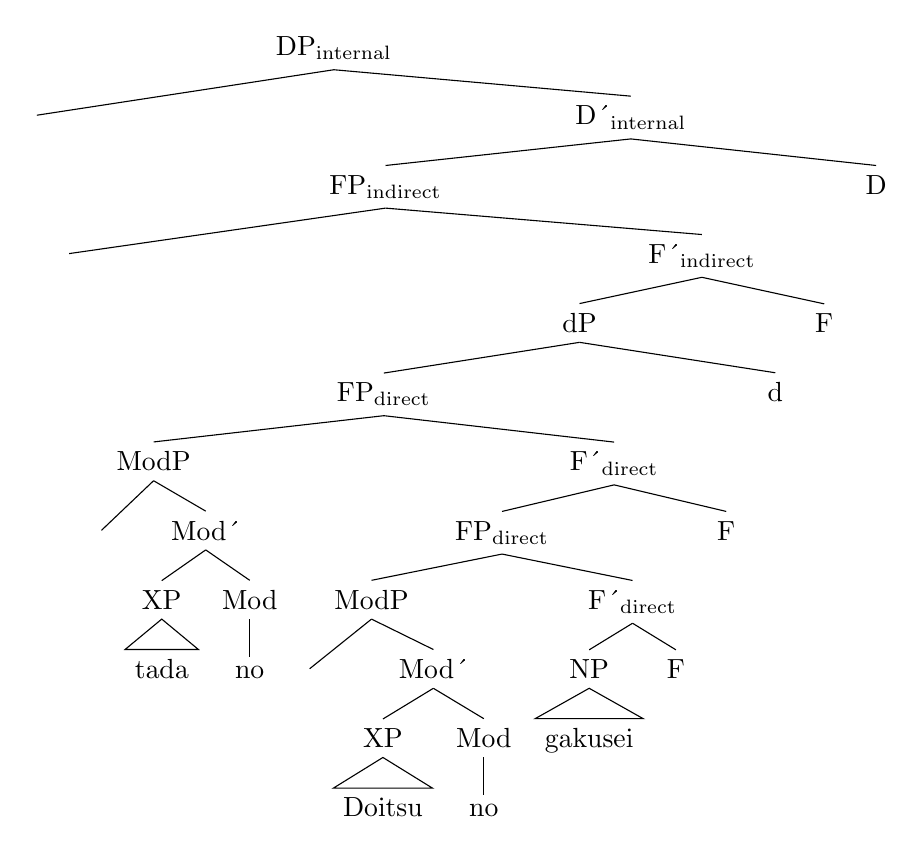
\begin{tikzpicture}[baseline=0pt, remember picture]
\tikzset{level distance=25pt, sibling distance=5pt}
\Tree [.DP\textsubscript{internal} {} [.D´\textsubscript{internal} [.FP\textsubscript{indirect} {} [.F´\textsubscript{indirect} [.dP [.FP\textsubscript{direct} [.ModP {} [.Mod´ [.XP \edge[roof]; tada ] [.Mod no ] ]] [.F´\textsubscript{direct} [.FP\textsubscript{direct} [.ModP {} [.Mod´ [.XP \edge[roof]; Doitsu ] [.Mod no ] ] ] [.F´\textsubscript{direct} [.NP \edge[roof]; gakusei ] F ] ] F ] ] d ] F ] ] D ] ]
\end{tikzpicture}

On the other hand, the reverse order \textit{Doitsu-no tada-no gakusei}, lit. `German mere student', ungrammatical in English, is a result of \textit{tada-no} ocupying a lower position.

\newpage

\ex. \ag. Doitsu-no tada-no gakusei\\
German-\textsc{mod} mere-\textsc{mod} student\\
`a mere German student' (= \ref{tada2})
\b. 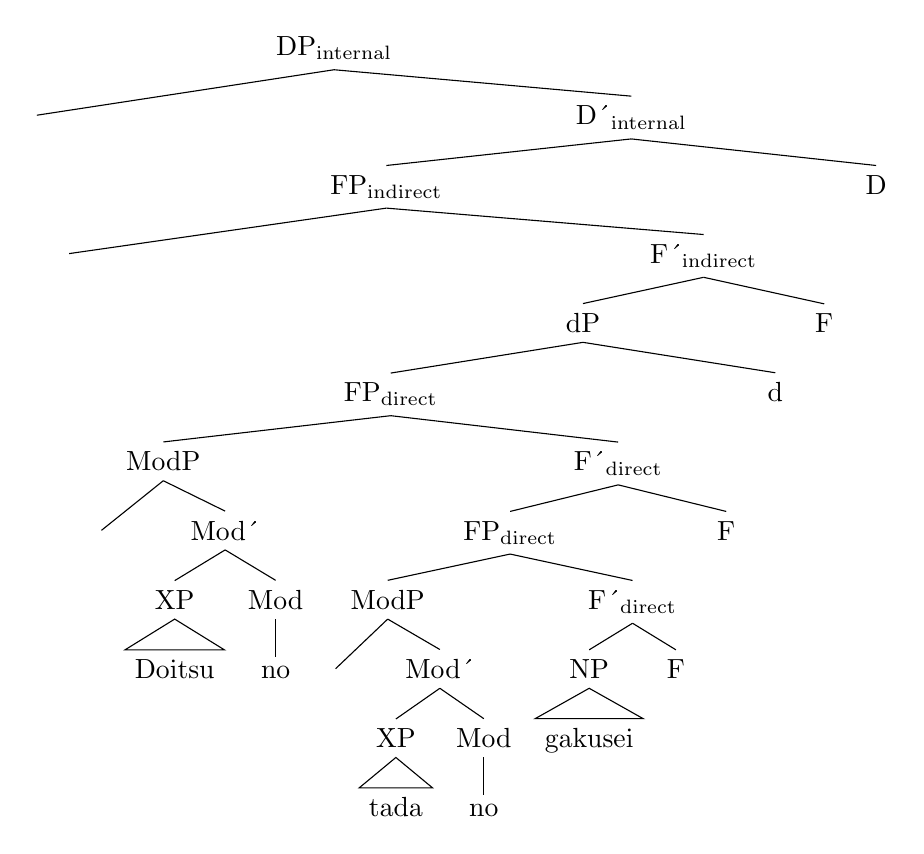
\begin{tikzpicture}[baseline=0pt, remember picture]
\tikzset{level distance=25pt, sibling distance=5pt}
\Tree [.DP\textsubscript{internal} {} [.D´\textsubscript{internal} [.FP\textsubscript{indirect} {} [.F´\textsubscript{indirect} [.dP [.FP\textsubscript{direct} [.ModP {} [.Mod´ [.XP \edge[roof]; Doitsu ] [.Mod no ] ]] [.F´\textsubscript{direct} [.FP\textsubscript{direct} [.ModP {} [.Mod´ [.XP \edge[roof]; tada ] [.Mod no ] ]] [.F´\textsubscript{direct} [.NP \edge[roof]; gakusei ] F ] ] F ] ] d ] F ] ] D ] ]
\end{tikzpicture}

Although both modifiers are situated in the direct domain, which has been verified viz. their status as direct modifiers, their exact position is not predetermined and this scenario is at stake for all direct modifiers with interchangeable ordering.

\subsection{Language variation in ordering} \label{language variation}

Assuming a broad direct domain explains the absence of ordering restrictions in Japanese. But it yet fails to explain stricter ordering restrictions in languages such as English or German, which over the years have justified the inventory of functional projections based on specific semantic categories \citep{cinque:2010:adj, cinque:2025:superiority, laenzlinger:2011:elements}. The question is: what makes Japanese so different from English, i.e. what determines whether a language has a broad domain with unspecific, or a more articulated domain with specific functional projections?

\subsubsection{Universal Spine Hypothesis and Units of Language} \label{units of language}

To answer these questions, I draw ideas from Wiltschko's \textit{Universal Spine Hypothesis} (USH, \citealt[24–26]{wiltschko:2014:universal})j, which offers a radically different perspective from cartography. I argue that this hypothesis enriches this research program in various ways and offers a solution to the questions presented above.\footnote{For the specific spine and its projections proposed by Wiltschko as an alternative to the ones proposed here, see \citet[ch. 2]{wiltschko:2014:universal}.} I adopt the following main ingredients (cf. \citealt[ch. 1, 2]{wiltschko:2014:universal}). %\is{Universal Spine Hypothesis} %\is{Units of Language}

%\newpage

\ex. \a. There is a universal syntactic spine which holds across all languages and is part of UG.
\b. Across this spine, we find a universal inventory of hierarchically ordered categories.
\c. Whether these categories surface in a specific language, however, is subject to language-specific factors.
\d. Each language has its own language-specific entities, called \textit{Units of Language} in \citet[1]{wiltschko:2014:universal}, which derive language-specific categories from universal categories.

The basic idea is as that of a universal DP-spine with three different domains and functional heads within these domains licensing modifiers and giving landing sites. This general DP-spine and its three domains are uniform cross-linguistically: the left periphery, the indirect domain, and the direct domain. The nature of the functional heads are shared with standard cartographic assumptions as well. Functional heads within the direct and indirect domain license direct and indirect modifiers respectively and the left periphery serves mainly as a landing site for modifiers which move there for various reasons.

Furthermore, while the general spine is fixed, and thus variation limited across domains cross-linguistically, variation in the architecture, and thus in the surface order, comes into play within the same domain and this variation is language-specific (for a similar idea in the clause see \citealt{ramchand:2014:deriving}). Specifically, depending on its language-specific inventory, or its Units of Language (UoLs; \citealt{wiltschko:2014:universal}), each language realizes the categories in each domain in a different way, albeit those differences are systematic.

Languages such as English possess the Units of Language to realize specific categories of direct modifiers such as \textsc{quality} and \textsc{color}. They then combine those with the cross-linguistic spine and inventory of functional projections for direct modifiers to form the language-specific categories F\textsubscript{QUALITY} and so on. These functional heads license the respective modifiers in the structure and are ordered hierarchically. In linear order, this predicts the fixed order of these direct modifiers. %\is{Universal Spine Hypothesis} %\is{Units of Language}

Japanese, on the other hand, lacks the specific Units of Language for \textsc{quality} and similar categories, therefore does not realize specific functional projections which license modifiers of \textsc{quality} and which are ordered hierarchically. However, the universal DP is shared and this includes the direct domain. The difference between the functional heads and projections this domain contains and those of the English type is that the former are unspecific, and not specified for modifiers of specific semantic meanings, word classes, or levels of gradability, and other factors. This means, the functional heads within the Japanese direct domain are also not ordered in a specific hierarchy, and this correctly predicts the absence of ordering restrictions on the surface.

From a cross-linguistic perspective, and a perspective of UG, this means that children must acquire the relevant Units of Language required by the language they are learning in order to see which categories need activating and are embedded into a hierarchy.

Nevertheless, it is evident that the general hierarchy of functional projections in a given domain, if a given language realizes them, is uniform as well, considering the fact that the cross-linguistically attested ordering restrictions exemplified by modifiers of different categories are very similar across languages and variation can be explained by the application of different movement operations \citep{cinque:2023:linearization, cinque:2025:superiority}. Therefore, the process of acquiring the relevant hierarchy is not random, but conditioned on acquiring the relevant functional categories. %\is{Universal Spine Hypothesis} %\is{Units of Language}

As argued in \citet{wiltschko:2014:universal}, the Universal Spine Hypothesis fares better than its alternatives in a lot of scenarios. The Universal Base Hypothesis (UBH) of early generativism \citep{chomsky:1965:aspects} assumes uniformity, universality and identical structural make-up across all languages, the very core idea of present cartography \citep[68]{cinriz:2010:carto}. However, it faces two concrete problems: The first are overly specific categories in a certain language that should be present in all languages, yet are not attested. Equally problematic are cases of missing universal categories in a specific language (cf. \citealt[10–19]{wiltschko:2014:universal} and ch. 2.), the exact problem observable in Japanese, when it comes to ordering, and essentially the problem of plenitude \citep{larson:2021:rethinking}.

The No Base Hypothesis (NBH), on the other hand, attributes a special status to all languages in the sense that every category is language-specific. There are several counter arguments to this hypothesis, but only considering the data points here, it would not explain why the category of direct modifiers is attested in almost every language and why we observe such similar patterns in ordering restrictions across languages. Such a striking commonality does not come about by chance, but instead by cross-linguistic grammatical factors. Without a grammatical baseline, \citet[19–23]{wiltschko:2014:universal} asks, how come learners of so many different languages all acquire the same patterns?

One might object that the Universal Base Hypothesis is, nevertheless, active in Japanese, but that this language makes more use of movement than other languages. There is a logical problem with this objection. If there was an underlining order of modifiers, then we should be able to identify one order as the base order, or, alternatively, identify factors that ameliorate or deteriorate one order over the other. It should not be the case that both orders are equally perfectly acceptable. I.e., if we ask speakers, and especially if we look at corpus data, we should see that one order is still prevailing. That is because movement is always an additional option that the speaker has to perform and the listener has to parse. Therefore, I argue, the option of two different underlying orders is much more attractive than assuming one underlying order plus movement. %\is{Universal Spine Hypothesis} %\is{Units of Language}

Having established that Japanese lacks the language-specific inventories to realize fine-grained functional projections for direct-only modifiers, while languages such as English do realize said projections, leading to a strict marking of ordering in the latter language, the question is how far language variation is allowed. Can languages do whatever they want? Or are there some principles they have to adhere to? Taking the strict English-type and the loose Japanese-type as two extremes, one would expect that there is some ``middle-type'' or even a continuum across languages. This is essentially what is predicted by the claims made above. There should be languages that have the Units of Language for some categories but not for others.

If we find such a language, the next question is which intermediate levels of ordering emerge. That means, if some categories are ordered strictly, but some are not, which are ones that show strict ordering? Are they always the same or can they be different? Such an in-between language would offer the necessary data for a generalization. In the following, I will show that direct-only, non-intersective and relational modifiers, cross-linguistically are more likely to demand strict ordering, than qualitative modifiers, which are ambiguous in the first place in a lot of languages. In order to argue for this, I will focus on two languages in which qualitative modifiers are ordered quite freely, but once direct-only modifiers are involved, ordering restrictions apply. These languages will be Persian and Modern Greek. The reason for these choice are the existence of previous accounts on ordering in the DP in both languages and the comparatively easy testability.

\subsubsection{Persian} \label{persiananalysis}

I start the discussion with Persian.\footnote{Specifically Fārsi, the Persian variant spoken in Iran. I wish to thank Nasimeh Bahmanian very much for providing many of the examples and long discussions. For previous discussion and similar examples see also \citet{kahne:2014:revisiting}. However, some of his examples were judged as not so clear, which is why I elicited additional examples.} The relevant predictions are easy to test because modifiers with a few exceptions (demonstratives, superlatives, etc.) occur only postnominally. They are in this position always connected to the noun via the so called \textit{ezāfe}-morpheme (which in fact could be an instance of \textsc{mod} as it shows a similar distribution to \textsc{no}; see \citealt{toosarvandani:2014:the, gn:2024:morpho}). %\is{Universal Spine Hypothesis} %\is{Persian}

Like Japanese, but different from English, Persian does not show ordering restrictions among qualitative modifiers, illustrated with the familiar example of a \textsc{dimension} and a \textsc{color} modifier. Modifiers of these categories, which most likely have an adjectival status, are acceptable in either order in Persian and no order seems to be more grammatical or preferred over the other. %\is{Universal Spine Hypothesis} %\is{Persian}

%\newpage

\ex. \textsc{dimension} vs. \textsc{color}
\ag. miz-e qermez-e bozorg\\
table-\textsc{ez} red-\textsc{ez} big\\
\bg. miz-e bozorg-e qermez\\
table-\textsc{ez} big-\textsc{ez} red\\
`big red table'

Similar facts hold for modifiers of \textsc{material} and \textsc{dimension}, as well as \textsc{nationality} and \textsc{quality} respectively.

\ex. \textsc{dimension} vs. \textsc{material}
\ag. sandali-ye felezzi-ye bozorg\\
chair-\textsc{ez} metal-\textsc{ez} big\\
\bg. sandali-ye bozorg-e felezzi\\
chair-\textsc{ez} big-\textsc{ez} metal\\
`big metal chair'

\ex. \textsc{quality} vs. \textsc{nationality}
\ag. goldān-e qašang-e \v{z}āponi\\
vase-\textsc{ez} beautiful-\textsc{ez} Japanese\\
\bg. goldān-e \v{z}āponi-ye qašang\\
vase-\textsc{ez} Japanese-\textsc{ez} beautiful\\
`beautiful Japanese vase'

Note that modifiers of \textsc{material} and \textsc{nationality} can be used predicatively in Persian, in contrast to Japanese. Therefore, I analyze them as qualitative adjectives, analogous to the hierarchy of \citet{scott:2002:stacked}, albeit not as direct-only modifiers. %\is{Universal Spine Hypothesis} %\is{Persian}

\exg. Sandali felezzi ast / \v{z}āponi ast.\\
chair metal \textsc{cop} / Japanese \textsc{cop}\\
`The chair is metal(-ic) / Japanese.’

However, direct-only modifiers do exist and they demand ordering restrictions. This will be shown first for relational adjectives, labeled as such since they are in fact adjectival derivates from nouns, formed by the suffix -\textsc{i}. One example is \textit{haste’i} `nuclear’ derived from the noun \textit{haste} `nucleus, core’. This modifier, same as relational adjectives in other languages, cannot be used predicatively. %\is{Universal Spine Hypothesis} %\is{Persian} %\is{relational modifiers

\exg. *Fizikdān haste-i ast.\\
physicist nuclear-\textsc{ra} \textsc{cop}\\
(`The physicist is nuclear.’)

In \ref{fizikdan}, it is shown, with an example from \citet{kahne:2014:revisiting}, who draws the same conclusion, that the relational adjective has to occur closer to the noun than the qualitative adjective \textit{javān} `young’, which is not a direct-only adjective. The reversed order is illicit. Assuming the postnominal position is a result of NP-movement in a pied-piping fashion \citep{ross:1967:constraints, cinque:2010:adj}, the order of the postnominal modifiers reflects the mirror image of the underlying hierarchy. %\is{Universal Spine Hypothesis} %\is{Persian} %\is{relational modifiers

\ex. \label{fizikdan} \ag. fizikdān-e haste-i-ye javān\\
physicist-\textsc{ez} nuclear-\textsc{ra-ez} young\\
`young nuclear physicist'
\bg. *fizikdān-e javān-e haste-i\\
physicist-\textsc{ez} young-\textsc{ez} nuclear-\textsc{ra} \hfill \citep[18]{kahne:2014:revisiting}\\

In the following, I illustrate two more ordering pairs of relational and qualitative adjectives. In each case, the relational adjective must be adjacent to the head noun. Additionally, I show the illicit predicative use of the relational adjective.

\ex. \ag. doktor-e omun-i-ye javān\\
doctor-\textsc{ez} general-\textsc{ra-ez} young\\
`young general practicioner'
\bg. *doktor-e javān-e omun-i\\
doctor-\textsc{ez} young-\textsc{ez} general-\textsc{ra}\\
\cg. *Doktor omun-i ast.\\
doctor general-\textsc{ra} \textsc{cop}\\
(`The doctor is general.’)

\ex. \ag. kāx-e pādšāh-i-ye qašāng\\
palace-\textsc{ez} royal-\textsc{ra-ez} beautiful\\
`beautiful royal palace'
\bg. ??kāx-e qašāng-e pādšāh-i\\
palace-\textsc{ez} beautiful-\textsc{ez} royal-\textsc{ra}\\
\cg. *Kāx pādšāh-i ast.\\
palace royal-\textsc{ra} \textsc{cop}\\
(`The palace is royal.’)

Finally, when a relational adjective co-occurs with a non-intersective modifier such as \textit{qabli} `former’, also direct-only in Persian as shown in \ref{qabli}, the surface order is \textit{relational} $\succ$ \textit{non-intersective}. %\is{non-intersective modifiers} %\is{Persian} %\is{relational modifiers

\ex. \label{nuclearformer} \ag. dānešmand-e haste-i-ye qabli\\
scientist-\textsc{ez} nuclear-\textsc{ra-ez} former\\
`former nuclear scientist'
\bg. ??dānešmand-e qabli-ye haste-i\\
scientist-\textsc{ez} former-\textsc{ez} nuclear-\textsc{ra}\\

\exg. *Dānešmand qabli ast.\\
scientist former \textsc{cop}\\
(`The scientist is former.’) \label{qabli}

These facts are in line with the literature and findings in other languages. Recall that, truly non-intersective modifiers precede intersective direct modifiers in German and English (\citealt{trost:2006:das, panayidou:2013:in}; see Chapter \ref{ordering intersective}), suggesting a higher position for non-intersective modifiers. On the other hand, relational modifiers are hierarchically very low inside the direct domain (\citealt{bortolotto:2016:RA}; see Chapter \ref{ordering relational}). %\is{non-intersective modifiers} %\is{Persian} %\is{relational modifiers

In general, these findings suggest that Persian has the language-specific inventory to form specific projections for relational, and potentially non-intersective, modifiers, but that it lacks the inventory to realize specific functional projections reserved for qualitative modifiers of \textsc{dimension}, \textsc{quality} and so on. In other words, it possesses only the Units of Language responsible for direct-only modifiers (cf. also \citealt[18]{kahne:2014:revisiting}).

I therefore suggest that the direct domain in Persian looks as follows. The general DP structure is the same as in Japanese. Furthermore, the direct domain also contains several functional projections which are not based on specific categories, another characteristic shared with Japanese. The important point of deviation is that Persian does have certain functional projections which are based on specific categories, namely the projections that host relational adjectives. These are placed in a fixed position closer to the head noun. Tentatively, I also assume projections for non-intersective modifiers, which must be higher than those for relational modifiers, judging from \ref{nuclearformer}. Note that the surface order is the result of roll-up movement of the whose-pictures type after which all modifiers appear in the mirror-image order \citep{cinque:2017:micro, cinque:2023:linearization, kahne:2014:revisiting}. I do not display the \textit{ezāfe}-morpheme as a separate element, although it is also a very good candidate for a syntactic head selecting modifiers as also argued in \citet{philip:2012:linkers, toosarvandani:2014:the, franco:2015:linkers} and \citet{gn:2024:morpho}.\footnote{Intriguingly, some combinations of relational with qualitative adjectives were judged better in the unexpected order, potentially for unrelated reasons such as phonology and/or prosody. According to Nasimeh Bahmanian, the following example can be uttered in both orders, but interestingly, the qualitative adjective \textit{šadid} `severe’ seems to be a bit better closer to the head noun than the relational adjective \textit{zistmohiti} `environmental’.

\par

\ex. \ag. bohrān-e šadid-e zistmohit-i\\
crisis-\textsc{ez} severe-\textsc{ez} environmental-\textsc{ra}\\
\bg. bohrān-e zistmohit-i-ye šadid\\
crisis-\textsc{ez} environmental-\textsc{ra-ez} severe\\
`severe environmental crisis'

\par

}

\ex. DP-Structure for Persian\\
 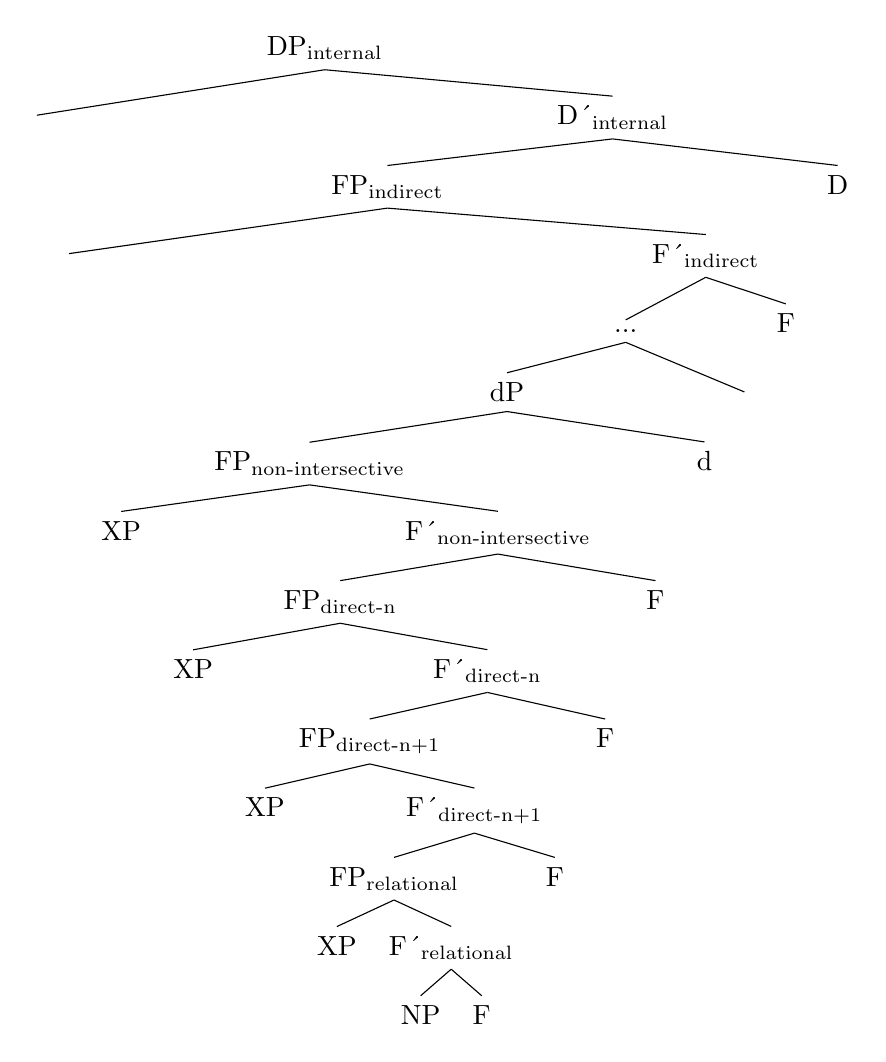
\begin{tikzpicture}[baseline=0pt, remember picture]
\tikzset{level distance=25pt, sibling distance=5pt}
 \Tree [.DP\textsubscript{internal} {} [.D´\textsubscript{internal} [.FP\textsubscript{indirect} {} [.F´\textsubscript{indirect} [.... [.dP [.FP\textsubscript{non-intersective} XP [.F´\textsubscript{non-intersective} [.FP\textsubscript{direct-n} XP [.F´\textsubscript{direct-n} [.FP\textsubscript{direct-n+1} XP [.F´\textsubscript{direct-n+1} [.FP\textsubscript{relational} XP [.F´\textsubscript{relational} NP F ] ] F ] ] F ] ] F ] ] d ] {} ] F ] ] D ] ]
\end{tikzpicture}

\subsubsection{Greek}

Modern Greek behaves similarly to Persian, although predictions are a bit more difficult to test.\footnote{I am very grateful to Jim Kotopoulis for providing the examples in this section and taking the time to discuss them with me. Unless indicated otherwise, the examples are his.} This is so because modifiers can, in principle, appear on both sides of the noun, and because they can appear with an additional determiner, a construction dubbed \textit{determiner spreading} \citep{androutsopoulou:1995:ds}. This option becomes necessary with postnominal modifiers \citep{alex:1998:adj, alex:2003:adj, campos:2004:ds, panagiotidis:2011:ds, lekakou:2012:poly, panayidou:2013:in}. An illustration is the following example where the two postnominal modifiers must occur with their own determiner. This is optional when they appear in prenominal position (adapted from \citealt[303]{alex:1998:adj}). %\is{Universal Spine Hypothesis} %\is{Greek} %\is{determiner spreading}

%\newpage

\ex. \ag. to vivlio *(to) kokino *(to) meghalo\\
\textsc{det} book \textsc{det} red \textsc{det} big\\
\bg. to meghalo (to) kokino (to) vivlio\\
\textsc{det} big \textsc{det} red \textsc{det} book\\
`the big red book’

Determiner spreading has often been argued to instantiate a case of predicative modification (see especially \citealt[A3]{cinque:2010:adj} and references therein), but matters are not so clear (see \citealt{lekakou:2012:poly} for examples of adjectives that are intersective but resist predicative use). Hence, I will limit myself to the relevant facts for the discussion. While free order of modifiers has often been pointed out in relevant structures, a welcoming fact for an analysis as indirect modifiers \citep{alex:1998:adj, alex:2007:nounphrase, cinque:2010:adj}, it seems to be the case that the order among standard categories of qualitative modifiers is also significantly less strict in structures not involving determiner spreading, compared to English or German. This is pointed out in \citet[174]{laenzlinger:2011:elements} and was confirmed by Jim Kotopoulis (p.c.). In the following example, as in Persian and Japanese, the modifiers of \textsc{dimension} and \textsc{color}, leaving factors such as focus, topicalization and emphasis aside, can appear in any order without deteriorating acceptability. Note that we only need to look at the prenominal position since in postnominal position, determiner spreading would be obligatory. %\is{Universal Spine Hypothesis} %\is{Greek} %\is{determiner spreading}

\ex. \textsc{dimension} vs. \textsc{color} 
\ag. to meghalo kokino vivlio\\
\textsc{det} big red book\\
\bg. to kokino meghalo vivlio\\
\textsc{det} red big book\\
`the big red book’

As in Persian, when direct-only modifiers are involved, a strict ordering can be observed. The surface order between the qualitative adjective \textit{neari} `young' and the relational adjective \textit{piriniki} `nuclear’, derived via the suffix -\textsc{i}, must be \textit{qualitative adjective} $\succ$ \textit{relational adjective} $\succ$ \textit{noun}, the reverse order \ref{piriniki neari} is ungrammatical. Crucially, \textit{piriniki} is impossible in constructions involving determiner spreading \ref{piriniki ds}, therefore can never appear postnominally \ref{piriniki post}. It is also not readily available in predicative position \ref{piriniki pred}. These facts are interconnected and underline its direct status.\footnote{According to Jim Kotopoulis, \textit{piriniki} can, in some instances, occur predicatively in which case it has a strong flavor of an elliptical construction. One reason for this might be that, contrary to English, Greek does not need an article when a noun appears predicatively, so only the noun needs to be deleted. A similar phenomenon in Japanese was shown at the beginning of this chapter.} %\is{Universal Spine Hypothesis} %\is{Greek} %\is{relational modifiers}

%\newpage

\ex. relational vs. qualitative modifier
\ag. i neari piriniki fisikos\\
\textsc{det} young nuclear physicist\\
`the young nuclear physicist'
\bg. *i piriniki neari fisikos\\
\textsc{det} nuclear young physicist \label{piriniki neari}\\
\cg. *i piriniki i fisikos\\
\textsc{det} nuclear \textsc{det} physicist \label{piriniki ds}\\
(`the nuclear physicist’)
\dg. *i fisikos i piriniki\\
\textsc{det} physicist \textsc{det} nuclear \label{piriniki post}\\
(`the nuclear physicist’)
\eg. *I fisikos ine piriniki.\\
\textsc{det} physicist \textsc{cop} nuclear\\
(`The physicist is nuclear.’) \label{piriniki pred}

An intriguing case is made by the modifier \textit{theatriki} `theatrical’, for example modifying the noun \textit{parastasi} `play’. \textit{Theatriki} can (at least for some speakers including Jim Kotopoulis) occur in determiner spreading-structures, but only in prenominal position, never postnominally \ref{parastasi post}. Furthermore it can appear in predicative position \ref{parastasi pred}.

\ex. \ag. i theatriki (i) parastasi\\
\textsc{det} theatrical \textsc{det} play\\
`the theatrical play’
\bg. *i parastasi i theatriki\\
\textsc{det} play \textsc{det} theatrical \label{parastasi post}\\
\cg. I parastasi ine theatriki.\\
\textsc{det} play \textsc{cop} theatrical\\
`The play is theatrical.’ \label{parastasi pred}

Nevertheless, even when determiner spreading is invoked, there are still ordering restrictions observed when it co-occurs with a qualitative adjective such as \textit{orea} `nice’. Then, \textit{parastasi} has to occur closer to the noun. I show this below for a DP without \ref{orea no ds}, and a DP with determiner spreading \ref{orea ds}.

\ex. \ag. i orea (i) theatriki (i) parastasi\\
\textsc{det} nice \textsc{det} theatrical \textsc{det} play\\
`the nice theatrical play’
\bg. *i theatriki orea parastasi\\
\textsc{det} theatrical nice play \label{orea no ds}\\
\cg. *i theatriki i orea (i) parastasi\\
\textsc{det} theatrical \textsc{det} nice \textsc{det} play \label{orea ds}\\

These facts are highly challenging for existing theories. They suggest that the same, or at least a similar, inventory of Units of Language is at stake for direct modification in Greek as in Persian. Both languages, then, do not have in their inventory functional projections dedicated to categories of qualitative modifiers such as \textsc{dimension}. However, they do realize functional projections dedicated to specific direct modifiers, namely relational modifiers. This explains the observed ordering principles. The DP structure for these two languages should thus look quite similar. %\is{Universal Spine Hypothesis} %\is{Greek} %\is{determiner spreading}

A remaining question is how cases in Greek can be explained where one, presumably direct, modifier occurs prenominally and another one occurs postnominally with determiner spreading.

\exg. i piriniki fisikos i neari\\
\textsc{det} nuclear physicist \textsc{det} young\\
`the young nuclear physicist’

This receives a nice explanation under the structure presented here and the assumption of two DPs (as also argued in \citealt{laenzlinger:2011:elements}), a lower position of the relational modifier and a combination of two movement operations. The underlying structure is presumably the following. Assuming \textit{piriniki} is a direct modifier, it is merged in the direct domain, thus lower in the DP. The exact status of \textit{neari} cannot be determined, but it seems to be higher in any case. %\is{pied-piping} %\is{determiner spreading}

\newpage

\ex. \begin{tikzpicture}[baseline=0pt, remember picture]
\tikzset{level distance=25pt, sibling distance=5pt}
 \Tree [.DP\textsubscript{external} {} [.D´\textsubscript{external} {} [.FP {} [.F´ F [.AgrP {} [.Agr´ Agr [.DP\textsubscript{internal} {} [.D´\textsubscript{internal} i [.AgrP \node (voitures2) {}; [.Agr´ Agr [.FP [.AP \edge[roof]; neari ] [.F´ F [.AgrP \node (voitures3) {}; [.Agr´ Agr [.FP\textsubscript{direct} [.AP \edge[roof]; piriniki ] [.F´ F [.NP \edge[roof]; \node (voitures4) {fisikos}; ]]]]]]]]]]]]]]]]]
 \end{tikzpicture}

The derivation likely proceeds as follows: First the NP moves in a pictures-of-whom type movement operation to the specifier of a higher functional head (AgrP in \citealt{cinque:2017:micro, cinque:2023:linearization}), dragging along the relational modifier \textit{piriniki}, but crucially not affecting the order. Then this chunk moves across the qualitative modifier \textit{neari} to the left periphery across the determiner. Crucially, this modifier remains in-situ and we get the order \textit{piriniki} $\succ$ \textit{fisikos} $\succ$ \textit{i} $\succ$ \textit{neari}. Next, the determiner moves to the DP-external domain and leaves a copy in the internal DP, as, for instance, argued in \citet{laenzlinger:2011:elements} and see \citet{grohmann:2003:prolific, grohmann:2015:demonstrative}. %\is{pied-piping}

\subsubsection{Summary}

The preceding discussion has shown that the DP structure presented in this study is applicable to other languages, emphasizing its universal status, but that parametric variation is permitted. Importantly, this variation is not random. There are languages which do not show ordering restrictions of categories such as \textsc{quality}, but do show ordering restrictions when it comes to direct-only modifiers. On the other hand, the reverse case is (at least so far) missing from the paradigm. Languages such as English or German show ordering restrictions in all scenarios. 

On the basis of these facts, I propose the following generalization. %\{Generalization on Cross-Linguistic Ordering Restrictions}

\ex. \emph{Generalization on Cross-Linguistic Ordering Restrictions}\\
If a language shows ordering restrictions among qualitative modifiers such as \textsc{quality} and \textsc{dimension}, it will also show ordering restrictions among direct-only modifiers, for example relational and non-intersective modifiers, among each other and with other categories. In other words, if a language has the language-specific inventory to realize functional projections for categories of \textsc{quality}, \textsc{dimension}, etc., it will also realize functional projections for direct-only modifiers.

This means that there are indeed languages between the English type, in which all categories adhere to specific, preferred orders in context-neutral utterances, and the Japanese type, in which there is the same universal spine observable, but not the language-specific entities for functional projections of fine-grained semantic categories. It is for future researchers to prove or refute this claim and to see whether more points can be added to the continuum and whether an even more fine-grained generalization can be put forth.

\subsubsection{Two more languages} \label{more languages}

Before closing this subsection, I would like to draw attention to two languages that prove the above made claim in different ways. First, \citet{brown:2024:adj} shows that in Naasioi, a Papuan language, direct adjectives do not adhere to ordering restrictions. Adjectives in this language can appear pre- or postnominally, seemingly without restrictions. Furthermore, direct can be differentiated from indirect adjectives via presence of an additional article in the latter case, making this construction appear very similar to determiner spreading in Modern Greek. First, direct modifiers must appear closer to the noun than indirect modifiers, illustrated in N-A-A sequences below. %index: Naasioi

\ex. \ag. Te mosi pangkaing te mutaanu aatu-maang. (Naasioi)\\
\textsc{det} dog big \textsc{det} black sleep-\textsc{prs.prog}\\
`The big dog which is black is sleeping.’
\bg. *Te mosi te mutaanu pangkaing aatu-maang.\\
\textsc{det} dog \textsc{det} black big sleep-\textsc{prs.prog}\\ \null \hfill \citep[432]{brown:2024:adj}

Assuming all modifiers that appear without the additional article \textit{te} are direct, they should adhere to ordering restrictions in contexts with two or more direct modifiers. Alas, they do not, as \citet{brown:2024:adj} argues based on fieldwork data. This generalization seems to hold, at least, for modifiers of \textsc{dimension}, \textsc{color} and \textsc{quality} at least and is exemplified below with a string of three adjectives, which, according to \citet{brown:2024:adj} are fine in either order.

\exg. Te orara pangkaing arasi kiring dua-’ar-ing.\\
\textsc{det} bad big brown breadfruit fall-\textsc{pl-imm.pst}\\
`The bad big brown breadfruits fell.’

In other words, this language poses a problem for standard cartography as well. In fact, since it seems to pattern with the languages depicted above (although no immediate conclusion can be drawn about relational and nonintersective modifiers), the same facts seem to be at stake, namely a direct domain with unspecific projections, in which various movement operations can take place.

Containment relations akin to the one presented for Persian and Greek are given for Ojibwe, an Algonquian language, in \citet{rosen:2016:on}. This language seems to have a small class of direct modifiers, which are prenominally bound to the noun. The interesting part is that pairs of direct adjectives of \textsc{color} and \textsc{nationality} as well as \textsc{color} and \textsc{dimension} do not adhere to ordering restrictions, but pairs of \textsc{dimension} and \textsc{nationality} must do so (\textsc{ni} = inanimate noun).

\ex. \textsc{color} vs. \textsc{nationality}: No ordering restrictions
\ag. misko-Anishinaabe-mashkimod\\
red-Ojibwe-bag.\textsc{ni}\\
\bg. Anishinaabe-misko-mashkimod\\
Ojibwe-red-bag.\textsc{ni}\\
`a red Ojibwe bag’ \null \hfill \citep[161]{rosen:2016:on}

\ex. \textsc{dimension} vs. \textsc{color}: No ordering restrictions
\ag. gichi-misko-waakaa’igan\\
big-red-house.\textsc{ni}\\
\bg. misko-gichi-waakaa’igan\\
red-big-house.\textsc{ni}\\
`a big red house’ \null \hfill \citep[161]{rosen:2016:on}

\ex. \textsc{dimension} vs. \textsc{nationality}: Ordering restrictions
\ag. gichi-Anishinaabe-mashkimod\\
big-Ojibwe-bag.\textsc{ni}\\
`a big Ojibwe bag’
\bg. *Anishinaabe-gichi-mashkimod\\
Ojibwe-big-bag.\textsc{ni} \null \hfill \citep[162]{rosen:2016:on}\\

Furthermore, for some reason, \textsc{nationality} adjectives can appear to the left of \textsc{dimension} adjectives if an adjective of \textsc{color} intervenes \citep[162]{rosen:2016:on}.

\exg. Anishinaabe-misko-gichi-adoopowin\\
Ojibwe-red-big-table.\textsc{ni}\\
`a big red Ojibwe table’ \null \hfill \citep[162]{rosen:2016:on}

This order string \textsc{nationality} $\succ$ \textsc{color} $\succ$ \textsc{dimension} is the mirror-image order of modifiers compared to their assumed merge position. Naturally, it is unforeseen by any hierarchy. It should be impossible with modifiers in prenominal position according to Greenberg’s U20 and cannot be explained if we adopt the assumption that only the lexical head, the noun, can move. In other words, this surface order can only be explained if either, individual movement of modifiers, or, unspecific functional projections and free Merge positions are assumed. However, the latter assumption would have the big disadvantage that the strict order \textsc{dimension} $\succ$ \textsc{nationality} is unaccounted for.

Needless to say more work is necessary here, but one, very tentative, conclusion could be that, all things being equal, this language also does not realize functional heads based on specific semantic categories explaining the, in most cases, free order. However, there is a ban on the merge order of a modifier of \textsc{dimension} followed by a modifier of \textsc{nationality}  explaining why a string of two adjacent modifiers of those categories in that order is never available. I thus interpret these facts similar to the Japanese case, but with the twist that modifiers of \textsc{dimension} might never be merged directly after modifiers of \textsc{nationality}.

\subsection{Remaining questions} 

This section discusses two remaining question, namely whether there is complete freedom of ordering in Japanese, and whether complex direct modifiers do exist.

\subsubsection{\#1: Is there complete optionality in ordering?} \label{optionality}

If Japanese is a language, potentially one of many, with a broad direct domain lacking specific functional projections to dictate ordering, does that mean that no ordering principles exist at all? In other words: Is ordering of modifiers completely optional in this language? It was established that the semantic category of a modifier cannot be a factor, but in the following, I discuss potential other factors.

\newpage

\emph{Word Class/Morphology}

\par


I took care in balancing out the word classes that I tested for ordering preferences. Not only do the two Japanese adjective groups not adhere to ordering restrictions within and across one another \citep{kohlich:2018:die}, the present study showed that direct \textit{no}-modifiers, not only among one another, but also together with \textit{i}- and \textit{na}-adjectives, also do not lead to any ordering preferences in speakers. This clearly suggests the absence of the factors \textit{word class} or \textit{morphology}, which readers can verify in the examples above.

\emph{Phonology}

\par


It has been argued in \citet{nagano:2016:are} that phonology might play a role for ordering of modifiers, which is exactly why I have chosen to test modifiers with different amounts of morae. As it turns out, phonology does seem to be a factor, but only to a limited extent. For example, in none of the pairs \textit{Denmāku-no} `Denmark, Danish’ vs. \textit{chīku-no} `teak’ (5 vs. 3 morae) or \textit{ao-i} `blue’ vs. \textit{Chūgoku-no} `China, Chinese’ (2 vs. 4 mora) did ordering restrictions emerge. Note that I counted mora without the monomoraic elements following. %\is{mora length}

The only strict ordering seems to be dictated by the single monomoraic modifier of \textsc{material} \textit{ki-no} `wood(-en)’. Recall the example given in \citet{watanabe:2012:direct}, who argues that the combination with a trimoraic modifier leads to ungrammaticality if it is not placed closest to the noun. The relevant example is repeated from \ref{hokuo} below.

\ex. \ag. hokuō-no ki-no isu \\
North.Europe-\textsc{mod} wood-\textsc{mod} chair\\
`North European wooden chair' 
\bg. *ki-no hokuō-no isu\\
wood-\textsc{mod} North.Europe-\textsc{mod} chair \hfill \citep[508]{watanabe:2012:direct} \\

Now, this extends to the combination of \textit{ki} `wooden’ with other modifiers. The speakers I consulted prefer \textit{ki-no} closer to the head noun, but do not find the opposite example to be completely ungrammatical, just very marked. This is shown below. %\is{mora length}

\ex. \ag. Denmāku-no ki-no isu\\
Denmark-\textsc{mod} wood-\textsc{mod} chair\\
\bg. \#ki-no Denmāku-no isu\\
wood-\textsc{mod} Denmark-\textsc{mod} chair\\
`Danish wood chair'

Note that it really is phonology that is the factor at stake here, not semantic category, as the equivalent \textit{mokusei-no} `wooden’ is possible in either position and not marked.

%\newpage

\ex. \ag. Denmāku-no mokusei-no isu\\
Denmark-\textsc{mod} wooden-\textsc{mod} chair\\
\bg. mokusei-no Denmāku-no isu\\
wooden-\textsc{mod} Denmark-\textsc{mod} chair\\
`Danish wood chair'

While this means that phonology does have an effect on ordering to a certain extent, it is questionable how big its effect actually is. As noted, \textit{ki-no} is the only monomoraic modifier in the data set. This means that we cannot test similar modifiers to establish strict paradigms. On the other hand, with bimoraic modifiers such as \textit{ao-i} `blue’, I did not detect such an effect.\footnote{A comment made by an anonymous reviewer, alongside a provided example, fits well with this observation. According to their judgment the following minimal pair, with a bimoraic modifier of \textsc{nationality} does, all things being equal, also not offer a contrast.

\par

\ex. \ag. Tai-no mokusei-no isu\\
Thailand-\textsc{mod} wooden-\textsc{mod} chair\\
\bg. mokusei-no Tai-no isu\\
wooden-\textsc{mod} Thailand-\textsc{mod} chair\\
`Thai wood chair'

\par}

\emph{Pragmatic Factors, Scope}

\par


As already mentioned in Chapter \ref{japanesedp}, the only cases in which fixed order emerge involve different scope readings. In \ref{example scope}, the speaker is restricting the domain of German vases, not the domain of vases \textit{per se} to a concrete \textit{German vase} of which only one is available in the discourse. The reverse order, given the same context, is significantly degraded. %\is{scope}

\ex. \label{example scope} \ag. yui'itsu-no Doitsu-no kabin\\
only-\textsc{mod} German-\textsc{mod} vase\\
`the only German vase'
\bg. ??Doitsu-no yui'itsu-no kabin\\
German-\textsc{mod} only-\textsc{mod} vase\\

This is thus a case in which the two modifiers occupy distinct merge positions (at least in relation to one another, the precise projection being not important), although both inside the direct domain, as illustrated below.

\newpage

\ex. 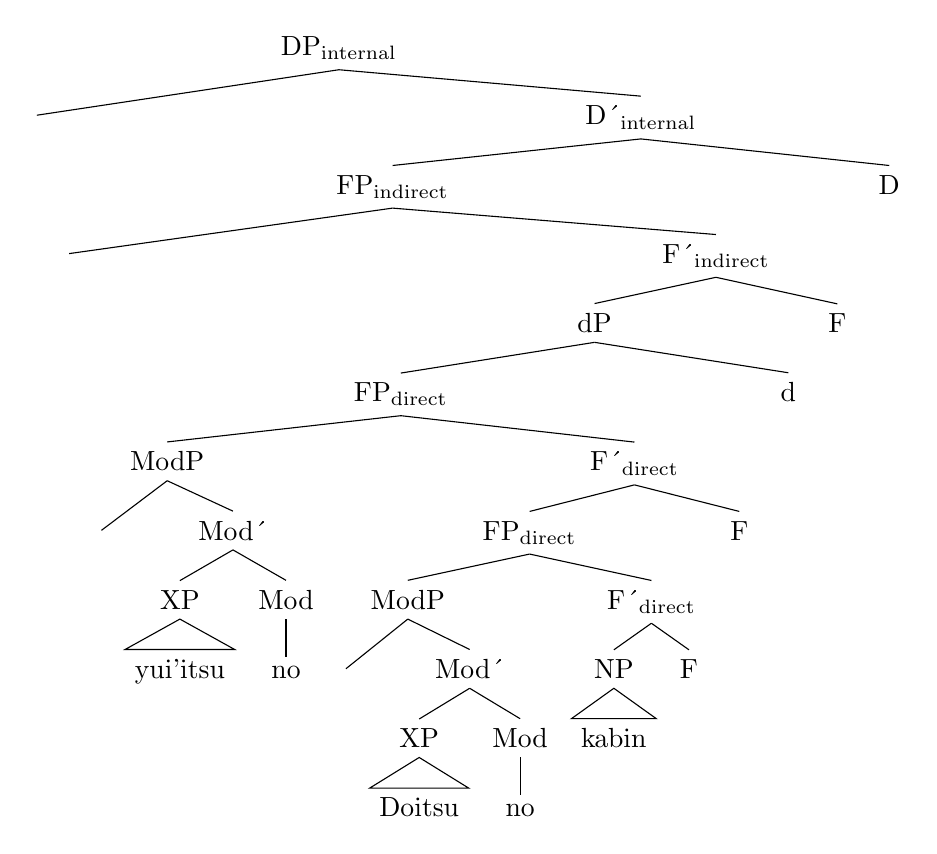
\begin{tikzpicture}[baseline=0pt, remember picture]
\tikzset{level distance=25pt, sibling distance=5pt}
\Tree [.DP\textsubscript{internal} {} [.D´\textsubscript{internal} [.FP\textsubscript{indirect} {} [.F´\textsubscript{indirect} [.dP [.FP\textsubscript{direct} [.ModP {} [.Mod´ [.XP \edge[roof]; yui'itsu ] [.Mod no ] ]] [.F´\textsubscript{direct} [.FP\textsubscript{direct} [.ModP {} [.Mod´ [.XP \edge[roof]; Doitsu ] [.Mod no ] ]] [.F´\textsubscript{direct} [.NP \edge[roof]; kabin ] F ] ] F ] ] d ] F ] ] D ] ]
\end{tikzpicture}

Connected to this is the strong nominal character of modifiers of \textsc{nationality}. Some, but not all, speakers reported that the second order to them suggests a reading like `the only vase IN Germany’. This also becomes obvious when combining such modifiers with possessive modifiers as in the following. Here, speakers again find a specific order more natural when they want to identify the particular referent: That in which the \textsc{nationality} modifier is closer to the noun.

\ex. \ag. watashi-no Doitsu-no kabin\\
I-\textsc{mod} German-\textsc{mod} vase\\
`my German vase(-s)’
\bg. ??Doitsu-no watashi-no kabin\\
German-\textsc{mod} I-\textsc{mod} vase\\

Seemingly, scope is at play again. The possessive modifier \textit{watashi-no} `my’ takes scope over \textit{Doitsu-no kabin}, not just \textit{kabin} alone, restricting the domain to a specific vase, namely one belonging to the speaker. Again, the reverse order does not involve scope and means something like `my vase(-s), which happen(s) to be in German / form/in Germany’.

These facts highlight that ordering in Japanese is not completely unrestricted, but that there are influencing factors, among them, to a minor extent, phonology, and, to a larger extent, scope restrictions. Importantly, these factors mostly seem to be \textit{syntax-external}, as also reported for similar cases in the clause in \citet{ramchand:2014:deriving}. Another such factor, presented in Chapter \ref{complexity} for indirect modifiers, is \textit{complexity}. This factor might not be really testable for direct modifiers, one of whose defining characteristics is to be, generally, less complex than their indirect counterparts. However, a related phenomenon will be discussed in the next section. 

\subsubsection{\#2: Complex direct modifiers and the situation in Classical Japanese} \label{complexdirect}

Another remaining issue to address concerns the possible existence of complex, that is clausal, direct modifiers. It is one of the characteristics of direct modifiers that they exhibit a less complex structure than indirect modifiers, which are arguably always embedded in a CP (\citealt{cinque:2010:adj, cinque:2020:relcl}, see Chapter \ref{indirect mod}). However, there is reason to believe that direct modifiers can also be complex. First, direct modifiers are not only functional, but can also be \textit{phrasal}. Evidence for this comes from the fact that direct adjectives can, in some languages, appear with overt adjectival arguments or adjuncts. This is shown below with an example from Bulgarian involving the direct (non-intersective) adjective `main’ and a prepositional complement (cf. \citealt[ch. 4.1.2]{cinque:2010:adj} for more data). %\is{complex direct modifiers} %\is{Bulgarian}

\exg. glavnata po zna\v{c}enie pri\v{c}ina (Bulgarian)\\
main.the in significance reason\\
`the main reason for importance’ \null \hfill \citep[47]{cinque:2010:adj}

In Japanese, some direct modifiers are clearly \textit{clausal}. This concerns especially structures in which such modifiers co-occur with an overt subject argument. Some relevant data points are given in \citet{hoshi:2002:kaynean}, who shows that some of the alleged examples of non-intersective modifiers given in \citet{yamakido:2000:japanese} do not only exhibit a predicative character, but also become intersective, highlighting this predicative character, when a subject appears (see \citealt{yamakido:2005:nature} for discussion). Observe \ref{hoshi example}. %\is{complex direct modifiers} %\is{non-intersective modifiers}

\exg. Pītā-wa [tsukiai-ga furu-i] tomodachi-da.\\
Peter-\textsc{top} association-\textsc{nom} long.time-\textsc{mod} friend-\textsc{cop}\\
`Peter has been a friend for a long time.’ (Lit.: `Peter is a friend whose association is old.’) \\ \null \hfill \citep[11]{hoshi:2002:kaynean} \label{hoshi example}

Here, the alleged direct modifier \textit{furu-i} `long.time’, which in combination with human entities only yields a non-intersective reading (Chapter \ref{non-intersective Japanese}), appears in a clausal structure with an overt subject. Furthermore, it now has acquired an intersective interpretation \textit{and} is possible in predicative position, evidenced in \ref{hoshi intersective}.

\exg. Pītā-wa [tsukiai-ga furu-i], soshite Pītā-wa tomodachi-da.\\
Peter-\textsc{top} association-\textsc{nom} long.time-\textsc{cop} and Peter-\textsc{top} friend-\textsc{cop}\\
`The association with Peter has been long and Peter is a friend.’ \\ \null \hfill \citep[11]{hoshi:2002:kaynean} \label{hoshi intersective}

Now admittedly, as has been argued, \textit{furu-i} can appear in predicative position as long as it is predicated on inanimate entities, which means it is not a direct-only modifier in the first place. However, a clausal construction is also possible for relational modifiers, as shown below for \textit{Chūgoku-no} `China, Chinese’. %\is{complex direct modifiers} %\is{relational modifiers}

\exg. seizōkoku-ga Chūgoku-no kuruma\\
country.of.production-\textsc{nom} China-\textsc{mod} car\\
`a car whose country of production is China’

In this case, the modifier also allows paraphrasing \textsc{no} with \textsc{de-ar-u} and inflection for past.

\ex. \ag. seizōkoku-ga Chūgoku-de-ar-u kuruma\\
country.of.production-\textsc{nom} China-\textsc{pred-cop-prs} car\\
`a car whose country of production is China’ 
\bg. seizōkoku-ga Chūgoku-d-at-ta kuruma\\
country.of.production-\textsc{nom} China-\textsc{pred-cop-pst} car\\
`a car whose country of production was China’

Two things are of importance here: Again, note that the modifiers in the preceding examples, different from the examples in \citet{cinque:2010:adj}, are not only phrasal but clausal. Second, what \textit{Chūgoku} here actually refers to is the country \textit{China}, but not the notion \textit{from China} as in examples such as \textit{Chūgoku-no kabin} `Chinese vase’ presented in Chapter \ref{RAJapanese}. \textit{Chūgoku-no} is \textit{per se} not a direct-only modifier either. %\is{complex direct modifiers} %\is{rentaishi}

More tricky is the following example with the \textit{rentaishi} \textit{ōki-na} `big’, which, different to \textit{ōki-i}, cannot appear in predicative position. However, it can take a subject argument in attributive position.

\exg. yane-ga ōki-na ie\\
roof-\textsc{nom} big-\textsc{mod} house\\
`house whose roof is big’ \\ \null \hfill \label{yane}

This means, the structural make-up, at least on the surface, for such constructions is similar to the following example, repeated from Chapter 3.

\exg. kami-ga kirei-na hito\\
hair-\textsc{nom} pretty-\textsc{mod} person\\
`a person whose hair is pretty' \null \hfill \citep[34]{kaplan:1995:the}

The question is how to analyze such cases. An interesting option is the notion of direct clausal modifiers, i.e. relative clauses, which, to my knowledge, was only considered a possibility by \citet{kim:2019:syntax}. She offers the following example: %\is{complex direct modifiers} %\is{direct relative clauses}

\ex. Politicians [who make extravagant promises] aren’t trusted. \\ \null \hfill \citep[139]{kim:2019:syntax}

Since this relative clause, from a semantic point of view, fulfills the function of ``characterizing people who are known as politicians'' \citep[139]{kim:2019:syntax}, it has an individual-level, not a stage-level, reading. This reading, in turn, is associated with direct modification \citep{cinque:2010:adj}, same as ambiguous adjectives such as \textit{visible}. \citet{kim:2019:syntax} leaves open what the precise structure of such relative clauses and their integration into the DP is, and indeed it is unclear what kind of structure we should assign to DPs such as \ref{yane}.

I assume, parallel to what is assumed for indirect modifiers with overt subjects, that the modifier \textit{ōki-na} `big’ projects a CP, making available a subject position in Spec, IP and providing a landing site for the relative clause operator in Spec, CP ensuring that the relative clause head is also correctly interpreted clause-internally. The whole CP is licensed by \textsc{mod}, which is realized as no overt tense appears (Chapter \ref{indirect mod}). This is given below. %\is{operator movement}

\exg. [\textsubscript{ModP} [\textsubscript{CP} \textit{Op}\textsubscript{1} [\textsubscript{IP} yane-ga [\textsubscript{PredP} [\textsubscript{AP} ōki-]na]]]] ie\textsubscript{1}\\
{} {} Op {} roof-\textsc{nom} {} {} big-\textsc{mod} house\\
`house whose roof is big’

Taking into account the existence of complex, that is relative clause-like, direct modifiers, is intriguing, but would violate the definition of \textit{direct-only} adopted in this study forcing certain concessions. On the other hand, I do not see an immediately tenable alternative which, still, maintains the proposal here. For now, I leave this for future research.

Importantly, clausal modification is impossible for many of the prime examples of direct-only modifiers, for instance \textit{shōrai-no} `future’, which do not allow an overt subject argument DP-internally.

\exg. *Kare-ga seikō-ga shōrai-no purosakkāsenshu desu.\\
he-\textsc{nom} success-\textsc{nom} future-\textsc{mod} pro.soccer.player \textsc{cop.pol}\\
(`He is a professional soccer player whose success is (expected) in the future.’)

Furthermore, \ref{yane} could find another explanation which relates to the nature of \textit{ōki-na} as a \textit{rentaishi}. Recall that all verbally derived \textit{rentaishi} are fossilized in their attributive form (\textit{rentaikei}), and this also extends to adjectival \textit{rentaishi} co-occurring with the premodern copula \textit{nari}/\textit{tari}, inflected for -\textit{naru}/\textit{taru} respectively, and potentially \textit{na}. As also argued in Chapter \ref{kaplan}, the attributive form of verbs in Classical Japanese clearly projected a C layer. Evidence for this comes from the occurrence in embedded wh-questions where it served the role of the complementizer \citep{kinsui:1995:iwayuru, kaplan:1995:the, hiraiwa:2005:dimensions}. This suggests that such modifiers might indeed still project a CP-layer explaining the clausal behavior.\footnote{In this respect, note also the following example with a verbally derived \textit{rentaishi} and a nominal subject, which prompted discussions already in the middle of the 20th century. Several authors have argued that the transition from verb to \textit{rentaishi} had not been fully achieved accounting for the possibility of overt subjects. See \citet{sekine:1937:fukutaishi, matsushita:1976:kaisen}) and \citet{kieda:1938:koto}.

\par

\exg. kimi-ga iwayuru shingi\\
you-\textsc{nom} so-called loyalty\\
`your so-called loyalty' (Lit. `what you call loyalty’) \null \hfill \citep[1:28]{sekine:1937:fukutaishi}

\par

}

This discussion also extends to other \textit{rentaishi} in Modern Japanese such as \textit{aru} `a certain’. There are (at least) two analyses possible for such lexemes: Either, they are analyzed as \textit{bona fide} (but fossilized) direct modifiers which do not project a higher functional layer, which are, somehow, not licensed via \textsc{mod}. Under this analysis, the ending \textit{ru} is taken to be part of the stem. %\is{complex direct modifiers} %\is{rentaishi}

\ex. \ag. aru gakusei\\
certain student\\
`a certain student' (= \ref{aru})
\b. 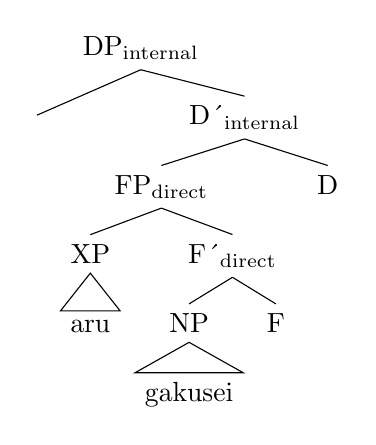
\begin{tikzpicture}[baseline=0pt, remember picture]
\tikzset{level distance=25pt, sibling distance=5pt}
 \Tree [.DP\textsubscript{internal} {} [.D´\textsubscript{internal} [.FP\textsubscript{direct} [.XP \edge[roof]; aru ] [.F´\textsubscript{direct} [.NP \edge[roof]; gakusei ] F ]] D ] ]
\end{tikzpicture}

Alternatively, staying closer to the structure such modifiers presumably had in Classical Japanese, they are direct modifiers, but project higher IP and CP layers. The ending \textit{ru} is the complementizer head. Note that I abstract away from the possible presence of \textsc{mod}.

\newpage

 \ex. \ag. a-ru gakusei\\
certain-\textsc{comp} student\\
`a certain student' (= \ref{aru})
\b. 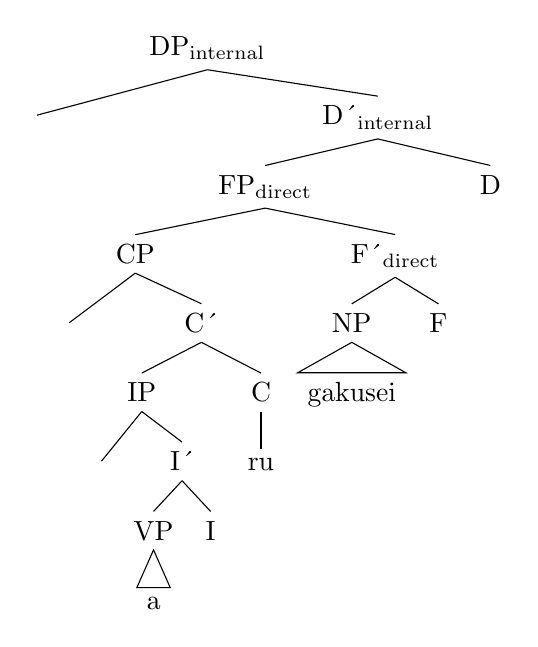
\begin{tikzpicture}[baseline=0pt, remember picture]
\tikzset{level distance=25pt, sibling distance=5pt}
 \Tree [.DP\textsubscript{internal} {} [.D´\textsubscript{internal} [.FP\textsubscript{direct} [.CP {} [.C´ [.IP {} [.I´ [.VP \edge[roof]; a ] I ] ] [.C ru ] ] ] [.F´\textsubscript{direct} [.NP \edge[roof]; gakusei ] F ]] D ] ]
\end{tikzpicture}

This discussion also concerns Classical Japanese, where all verbally and adjectivally derived lexemes analyzed as \textit{rentaishi} in Modern Japanese were still inflecting parts of speech in Classical Japanese. This means, in attributive position, they arguably could perform a role as direct modifiers casting doubt on the analysis of the attributive form (\textit{rentaikei}) in Classical Japanese -- although probably projecting a C layer (\citealt{kinsui:1995:iwayuru, kaplan:1995:the, hiraiwa:2005:dimensions}; cf. Chapter \ref{kaplan}) -- as being necessarily tied to indirect modification. Under this account, all modifiers had access to both kinds of modification at this stage of the language as well. For example, \textit{i}-adjectives, whose attributive form was represented via the suffix -\textsc{ki}, were presumably structurally ambiguous between an direct and an indirect status, similar to the situation in Modern Japanese. %\is{complex direct modifiers} %\is{Classical Japanese}

\exg. taka-ki mono\\
high-\textsc{rtk} thing\\
`a high thing' \null \hfill Classical Japanese

To summarize, the existence of clausal direct modifiers provides a challenge to the theory presented here, but could be explained via either, assuming the existence of complex direct modifiers, or, the special status of certain lexemes that are only direct in certain usage domains. A bigger challenge is posed by direct modifiers historically derived from verbs, and this extends to the situation in Classical Japanese. This is a fruitful area for future research.

\subsection{Summary}

In this section, I argued that Japanese lacks the language-specific categories to realize specific functional projections. This explains the lack of strict ordering and shows that direct modification and ordering are orthogonal issues. I then discussed the cross-linguistic implications of this claim and put forth a generalization on ordering principles. Finally, I showed that ordering in Japanese is in fact not entirely ungoverned either and discussed the possibility of complex direct modifiers.

\section{Chapter summary and closing remarks}

This chapter started with a discussion on why direct modification has so far been neglected, or entirely dismissed, in Japanese. Then, criteria for direct modification were introduced and it was shown that the lack of predicativity is the leading criterion, which is often accompanied by other criteria such as non-gradability. The following observations emerged in the course of the discussion:

\ex. \a. Japanese exhibits a variety of different direct-only modifiers: The equivalents of cross-linguistically well-known categories of non-intersective and relational modifiers, as well as cases of direct qualitative modifiers, idiomatic modifiers, direct quantificational modifiers and the language-specific group of \textit{rentaishi}.
\b. Almost all cases of direct-only modifiers are found among \textit{no}-modifiers.
\c. There is a lack of ordering restrictions which is due to a lack of projections dedicated to specific categories inside the direct domain.
\d. The reason for this is that Japanese does not have the language-specific entities to realize such dedicated functional projections.

I believe that the challenges these findings pose for cartography are also chances to expand this research field and adapt it in a way so that the very elaborate predictions it makes become even more powerful. Postulating a broader, more fluid set of functional projections inside the direct domain preempts the common criticism regarding superfluous projections as well as alleged violations of ordering restrictions. The concept of cross-linguistic variation enriches our understanding of the DP and generates new insights for other languages.

It is definitely a desideratum for future research to establish more cases of clear-cut ordering restrictions in Japanese, besides scopal relations or restrictions among direct and indirect modifiers. This would not only help expanding the hierarchy of direct modifiers proposed in this book in a language-specific and cross-linguistic perspective, but also could expand the structure of the direct domain I have proposed here and add a more fine-grained dimension to it.

\chapter{Indirect Modification in Japanese} \label{indirect japanese}

This chapter discusses the indirect domain and focus will be switched to indirect, that is predicative, modification. Although this kind of modification is often assumed to be the only one available in Japanese \citep{sproat:1991:the, baker:2003:verbal, laenzlinger:2011:elements}, no systematic analysis has been presented for indirect modifiers in this language, either. This concerns their fine-grained structure and the integration of this structure into the DP, their size and their position. This chapter thus aims at closing those research gaps and at broadening our understanding of this part of the DP, and indirect modifiers in Japanese and in general. After pointing out the characteristics of indirect modifiers in Japanese, I will discuss the issues mentioned above in turn. %\is{indirect modification}

\section{Introduction}

Recall that the indirect domain is situated inside the DP-internal domain, higher than the direct domain. It exhibits several functional projections for indirect modifiers as well as a projection that hosts numerals. As in the direct domain, these projections are not dedicated to a specific type of indirect modifiers, in this case to different sizes. The structure of the indirect domain inside the DP-internal domain is circled in the structure below.

\newpage

\begin{figure}[H]
\centering

 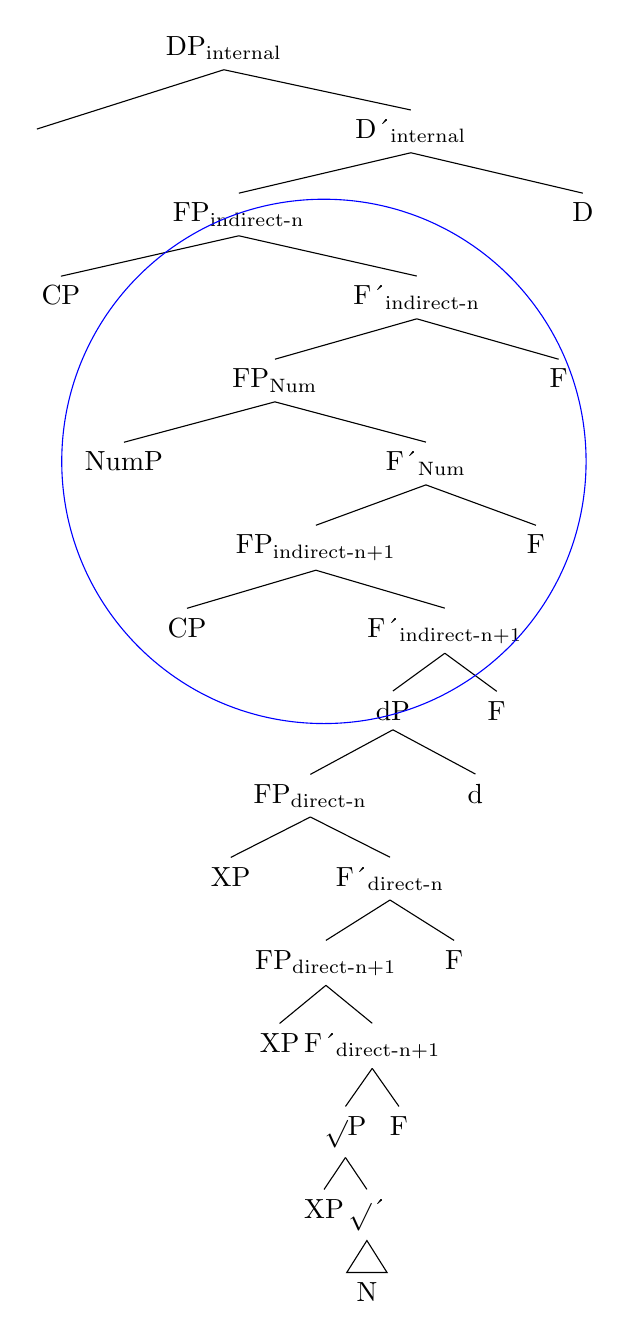
\begin{tikzpicture}[baseline=0pt, remember picture]
\tikzset{level distance=30pt, sibling distance=-5pt}
 \Tree [.DP\textsubscript{internal} {} [.D´\textsubscript{internal} [. \node (indirect1) {FP\textsubscript{indirect-n}}; CP [.\node (indirect0) {F´\textsubscript{indirect-n}}; [.FP\textsubscript{Num} NumP [.F´\textsubscript{Num} [.FP\textsubscript{indirect-n+1} \node (indirect3) {CP}; [. \node (indirect2) {F´\textsubscript{indirect-n+1}}; [.dP [.FP\textsubscript{direct-n} XP [.F´\textsubscript{direct-n} [.FP\textsubscript{direct-n+1} XP [.F´\textsubscript{direct-n+1} [.$\sqrt{}$P XP [.$\sqrt{}$´ \edge[roof]; N ] ] F ] ] F ] ] d ] F ] ] F ] ] F ] ] D ] ]
 \node[draw,circle,fit= (indirect0) (indirect3) ] [color=blue] {};
\end{tikzpicture}

 \caption{Structure of the indirect domain in Japanese}
 \label{fig:Structure of the indirect domain in Japanese2}
\end{figure}

%\newpage

\subsection{Goals and overview}

This chapter deals with the following questions relevant for indirect modifiers in Japanese:

\ex. \a. What are the complex morphological elements co-occurring with indirect modifiers, especially adjectives such as \textit{taka-katta} `was expensive', in Japanese?
\b. What is the size and merging position of indirect modifiers?
\c. What influences the position of indirect modifiers?

These questions will be addressed in turn and yield the following answers:

\ex. \a. The complex morphological elements such as \textsc{k-at-ta} are made-up of three elements: two copulas, and a tense morpheme. This analysis can be adapted to seemingly `simpler’ elements such as \textsc{da}.
\b. There is no difference in Japanese between full and reduced relative clauses; meaning indirect modifiers are only of one size: All relative clauses in Japanese are CPs and derived via operator movement \citep{miyamoto:2017:RC}.\footnote{In fact, nothing hinges on whether they have to be CPs or IPs (although CP-status grants a landing position for the operator). The important point is that relative clauses in Japanese only come in one size.}
\c. The only factor which has an effect on the position of modifiers inside the indirect domain is syntactic and prosodic complexity. More complex modifiers move to a position above numerals.

\subsection{Characteristics of Japanese indirect modifiers} \label{nishiyama analysis}

Recall that relative clauses are the prime example of indirect modifiers (\citealt{cinque:2010:adj, cinque:2020:relcl}; among others). In Chapter \ref{dP}, it was mentioned that languages such as English overtly display two types of relative clauses differing in size, structure and position, namely \textit{full} and \textit{reduced} relative clauses, but that this difference is generally hard to determine till non-existent in prenominal-RC languages. Such languages usually do not show two different types of relative clauses overtly, but, instead, exhibit other types of noun-modifying clauses that do not have direct counterparts as relative clauses in English and other well-known European languages \citep{keenan:1977:noun, lehmann:1984:der, vries:2002:syntax, wu:2011:syntax}.\footnote{For a coherent and contemporary typological overview of prenominal relative clauses see \citet{wu:2011:syntax}, who also points out that prenominal relative clauses ``have essentially only been studied in a few well-known and often-quoted languages such as Basque, Japanese, Mandarin, and Turkish" \citep[569]{wu:2011:syntax}.} %\is{indirect modification} %\is{relative clauses}

Japanese fits the description of other prenominal-RC languages. This language only exhibits one morphosyntactic type of relative clause, but it offers several constructions that do not correspond to relative clauses in European languages \citep{comrie:1998:rethinking, matsumoto:2017:japanese}. Furthermore, it exhibits the following characteristics which further complicate the analysis.

\newpage

\ex. \a. Lexemes exhibit (with the exceptions of nouns and \textit{na}-adjectives in non-past) no overt morphological difference between their role as modifier and in predicative position.
\b. Modifiers can exhibit a fairly complex morphological make-up in attributive position, again mirroring their predicative forms.
\c. Japanese exhibits a rather free word order within the DP, and this extends to indirect modifiers.
\d. Relative clauses can appear above demonstratives and can in principle be restrictive and non-restrictive in this position.

The observation that, with a few exceptions, the morphology of lexemes in attributive position is identical to the one displayed in predicative position further differentiates Japanese from other East Asian prenominal-RC languages. For example, looking at Mandarin (\textsc{de}), as well as other Sino-Tibetan languages, or Korean ( \textsc{(nu-)n}, relative clauses exhibit certain elements which connect them to the noun and which are absent in non-embedded root clauses. Japanese lacks such element. the surface form of an indirect modifier matches that of its predicative counterpart. This is, once more, exemplified below for a verbal relative clause.\footnote{It might be tempting to deduce the size of Japanese relative clauses from the fact alone that modifiers appear in a \textit{morphologically} \textit{finite} form. Already \citet[156]{keenan:1985:relcl} mentioned ``We may note that the prenominal RCs in Japanese do not put Vrel in a non-finite or specifically relative form, but the Japanese case appears to be the exception among prenominal RCs here’’. However, the notion of finiteness is not very well understood even in European languages and lacks a uniform definition. See the discussion in \citet{hudson:1973:tense, stanton:2011:rrc, belikova:2008:syntactically, belk:2017:attributes} with regard to reduced relative clauses in English, Dutch and Russian among others and \citet{nikolaeva:2007:intro} for an overview; see, for instance, \citet{wurmbrand:2005:infinitives, wurmbrand:2014:tense} and \citet{landau:2004:scale, landau:2013:control} for various phenomena in English.

The biggest obstacle is that finiteness can be approached from different perspectives. Overt tense is interpreted as morphological finiteness, especially in the Latin-Greek tradition. The classical syntactic understanding of finiteness is the assignment of nominative case \citep{chomsky:1981:lectures}, but also the morpho-syntactic marking of tense, person, politeness and other categories (see \citealt{nikolaeva:2007:intro} and articles therein). Its association with the C-domain has been put into question in recent literature as well, see \citet{adger:2007:finiteness, bisang:2007:finiteness} and especially \citet{wurmbrand:2020:finiteness}, who argue that it can be encoded at different levels of the clause, ranging from C to T even to v. From a semantic point of view, finiteness is related to the distribution of overt tense and the indication of the ``existence of a predication at the time of the utterance" \citep[201]{platzack:1995:loss}. As shown for example in \citet{ogihara:1994:adverbs} and \citet{miyagawa:2012:case}, Japanese relative clauses can, but do not need to, be dependent on the higher clause.

To summarize, finiteness is not helpful in determining the status and syntactic size of a relative clauses and will be sidelined here as a criterion. Nevertheless, note that I used the notion of finiteness, in the sense that tense is projected, to argue for the possible non-occurrence of realizations of \textsc{mod}.} %\is{finiteness}

\newpage

\ex. \ag. Kare-ga hon-wo kat-ta.\\
he-\textsc{nom} book-\textsc{acc} buy-\textsc{pst}\\
`He bought a book.’
\bg. kare-ga kat-ta hon\\
he-\textsc{nom} buy-\textsc{pst} book\\
`the book (which) he bought'

This extends to all non-verbal modifiers inflected for past. \textit{na}-adjectives and \textit{no}-modifiers can co-occur with the canonical copula forms \textsc{de-ar-u} and \textsc{d(e)-at-ta} both in attributive and predicative position, and \textit{i}-adjectives can co-occur with \textsc{k-at-ta} in order to show that they are inflected for past, as shown below.

\ex. \ag. Ano doresu-wa taka-k-at-ta.\\
that dress-\textsc{top} expensive-\textsc{pred-cop-pst}\\
`That dress was expensive.'
\bg. ano taka-k-at-ta doresu\\
that expensive-\textsc{pred-cop-pst} dress\\
`that dress which was expensive' \null \hfill \textit{i}-adjective, past

I will start with a discussion of these elements before discussing the size and position of indirect modifiers.

\section{The Elements PRED, COP and T} \label{copulaelements}

In this section, I present a precise analysis of the complex morphological elements Japanese modifiers can co-occur with. Following Nishiyama (\citealt{nishiyama:1999:adj}, and see also \citealt{miyama:2011:da, watanabe:2013:non, yamada:2023:looking}), I will step by step outline that they are composed of a predicative copula (\textsc{pred}) in the sense of \citet{bowers:1993:predication}, a dummy copula and a tense marker, starting with the final element, and translate the data into the cartographic structure adopted here. This analysis will then be applied to the shorter version of the copula, \textsc{i} and \textsc{da}, and I will explain why an adaption to the monomoraic elements occurring in attributive position is not justified. %\is{copula}

\subsection{Nishiyama's Analysis}

\subsubsection{Tense marker}

The final element \textsc{ta} contained in \textsc{k-at-ta} and \textsc{d(e)-at-ta} and also occurring with verbs straightforwardly receives an analysis as a tense marker for past.\footnote{\textsc{ta} is likely derived from the premodern auxiliary verb -\textit{tari}, which was added to the nominalization form of inflecting categories and was itself inflecting.} \textsc{ta} is subject to different phonological processes, namely gemination, and also devoicing yielding the allomorph /da/. The first generalization to be drawn is thus as follows. %\is{tense}

\ex. \textsc{ta} = \textsc{I} (past)

The analogous element for non-past is -\textsc{u}.\footnote{When /u/ is added to the stem of vowel-stem verbs such as \textit{tabe} `to eat’, an epenthetic alveolar /r/ is inserted. Note that there are also consonant-stem verbs whose stem ends in /r/ and which share their paradigm with the dummy copula (see below). In this case, the alveolar consonant is part of the stem. Before the past ending and the suffix -\textsc{te}, /r/ is deleted and /t/ is geminated. These groups of verbs should thus not be mixed up. They can be further differentiated based on their inflectional paradigms. For discussion see \citet[364–365]{ito:2015:word}. In any case, the morpheme signaling non-past remains the same.}

\ex. \textsc{u} = \textsc{I} (non-past)

\subsubsection{Dummy Copula}

When added to adjectives and \textit{no}-modifiers, \textsc{ta} is obligatorily preceded by the element \textsc{ar}, which Nishiyama analyzes as the dummy copula. In this sense, the copula is \textit{semantically vacuous}, a ``dummy element whose function is merely to support tense'' \citep[187]{nishiyama:1999:adj}. In thus performs a function of \textit{be}-support, similar to English \textit{do}-support.

This view goes, among others, back to \citet{bach:1967:have} and \citet{doron:1983:verbless} and was formalized in \citet{rapoport:1987:copular}. In English, the copula \textit{be}, although it can serve the semantically important function of identification (\textit{That woman is Tali.}; cf. \citealt[150]{rapoport:1987:copular}), is typically devoid of meaning, yet necessary in predicative and equative sentences involving non-verbal elements (examples based on \citealt[156]{rapoport:1987:copular}).

\ex. \label{nut} \a. Xeli *(is) a nut.
\b. Tali *(is) that woman over there.

As a contrast, it is not necessary in small clause predicational environments involving a lexical verb.

\ex. I consider Xeli a nut. \label{consider} \null\hfill \citep[152]{rapoport:1987:copular}

\citet{rapoport:1987:copular} first showed that there is no semantic requirement for the copula, that it is semantically empty, hence must be a syntactic element that satisfies a syntactic requirement. This requirement is that every sentence has to contain a verb, since every sentence needs to express tense \citep[157]{rapoport:1987:copular}. This can be achieved by a lexical verb \ref{consider}, or, alternatively, by the copula \ref{nut}. In absence of a verb, the copula supports the tense (and agreement) features of \textsc{I} (ibid.).\footnote{It does not become clear whether \textit{consider} indeed is a lexical verb in this analysis. See \citet{bowers:1993:predication} for an analysis of \textit{consider} and similar verbs in English.} %\is{copula}

In many languages, the semantically vacuous copula can be omitted in the default tense non-past/present, but is needed in other contexts, for example to express past where it bears tense inflection. This underlines its supporting character for the I node and lack of semantic contribution. Observe the following scenario in Russian (cf. \citealt{babby:2010:syntactic}; cf. \citealt{doron:1983:verbless, rapoport:1987:copular} for Hebrew). %\is{copula} %\is{Russian} %\is{Hebrew}

\ex. \label{pagoda} \ag. Pagoda xorošaja. (Russian)\\
weather.\textsc{nom.sg.f} good.\textsc{nom.sg.f}\\
`The weather is good.' \null \hfill present
\bg. Pagoda *(byla) xorošaja.\\
weather.\textsc{nom.sg.f} was.\textsc{sg.f} good.\textsc{nom.sg.f}\\
`The weather was good.' \null \hfill past

The semantically vacuous copula in Japanese is identified in \citet{nishiyama:1999:adj} and \citet{urushibara:1993:syntactic} as -\textsc{ar}- and given the syntactic label \textit{V}. To avoid confusion, I will use the label \textsc{cop}.\footnote{\citet{watanabe:2013:non} assigns the dummy copula the light verb status \textit{v}. Recall that before the past tense morpheme \textsc{ta}, obligatory gemination happens.}

\ex. \textsc{ar} = \textsc{cop}

\textsc{ar} can also be used as an independent verb, which expresses existence, identical to English \textit{be}. %\is{dummy copula}

\exg. Kuruma-wa niwa-ni ar-u.\\
car-\textsc{top} garden-\textsc{loc} \textsc{cop-prs}\\
`The car is in the garden.’

It also appears in other scenarios \textit{be} appears in, including equation \ref{equation} and identification \ref{identification}. In both case, another element, namely \textsc{de} (the predicative copula, see below) is required. %\is{dummy copula}

\exg. Hanako-wa sensei-de-ar-u.\\
Hanako-\textsc{top} teacher-\textsc{pred-cop-prs}\\
`Hanako is a teacher.' \label{equation}

\exg. Ano ko-wa Hanako-de-ar-u.\\
that girl-\textsc{top} Hanako-\textsc{pred-cop-prs}\\
`That girl over there is Hanako.' \label{identification}

It needs to be made clear that the sole, but very strong, piece of evidence that \textsc{ar} is a (dummy) copula is its requirement to support tense, in other words to host the tense node. Non-verbal elements can never express overt tense, with an overt non-past or past morpheme, without the presence of \textsc{ar}, as given below.

\newpage

\exg. *Ano doresu-wa shikku-(de)-u / (de)-ta.\\
that dress-\textsc{top} chic-\textsc{pred-prs} / \textsc{pred-pst}\\
(`That dress is/was chic.’)

This means, the dummy copula is a different element from \textsc{de}, which is not sufficient to support tense and will be reviewed below.

\subsubsection{Predicative Copula} \label{chapter pred}

However, a tense marker and the dummy copula are not enough to license an adjective or a \textit{no}-modifier in predicative position either. Additionally, the element \textsc{de}, in the case of \textit{na}-adjectives and \textit{no}-modifiers, or \textsc{ku}, in the case of \textit{i}-adjectives, are required. Following \citet{nishiyama:1999:adj}, I will analyze this element as another, a more meaningful kind of, copula, namely as the syntactic head for predication \textsc{pred} (\citealt{bowers:1993:predication}, there \textsc{pr}; cf.also \citealt{svenonius:1996:pred, bowers:2002:pred, dikken:2006:relators, heycock:2013:syntax}). This element is the real bearer of predication.\footnote{A similar view can also be found in the work of one of the first Western linguists specialized in Japanese: Bernard Bloch. Bloch assessed in the 1940's that the Japanese copula is an inflectional element and that every sentence needs such an inflectional element as its nucleus, making the copula an essential ingredient of the sentence (\citealt[35]{bloch:1970:bloch}, see \citealt[187–188]{nishiyama:1999:adj}).} %\is{predicative copula}

Evidence for this analysis and for the differences between the two copulas are visible in the following data points. Precisely, whenever a predication relation between a non-verbal \textit{na}-adjective or \textit{no}-modifier and a verb is established, the predicative copula obligatorily appears, but the dummy copula is absent. This is visible in \ref{overtpred}, where \textit{no}-modifiers are used as depictives of a verb. See especially \citet{koizumi:1995:secondary}, to whom most of these data points and observations can be attributed. %\is{predicative copula} %\is{depictives}

%\newpage

\ex. \label{overtpred} \ag. Jon-ga sakana-wo hadaka-*(de) tabe-ta.\\
John-\textsc{nom} fish-\textsc{acc} naked-\textsc{pred} eat-\textsc{pst}\\
`John ate the fish naked.' \null\hfill \citep[188]{nishiyama:1999:adj}
\bg. Jon-ga katsuo-wo nama-*(de) tabe-ta.\\
John-\textsc{nom} bonito-\textsc{acc} raw-\textsc{pred} eat-\textsc{pst}\\
`John ate the bonito raw.' \null \hfill \citep[27]{koizumi:1995:secondary}

In these examples, the predication relation is established via \textsc{pred}, which is spelled-out as /de/. While predication needs to be established, the tense node already has a host, namely, in both sentences the verb \textit{tabe} `to eat’. Therefore, the dummy copula is not needed. %\is{predicative copula} %\is{dummy copula}

This means the two copulas differ in the following ways:

\newpage

\ex. \a. The dummy copula is semantically meaningless, it is simply there to support tense. The predicative copula is the bearer of predication.
\b. The dummy copula cannot occur independently and is not required when a verb is present. The predicative copula can independently co-occur with modifiers in tenseless environments, in which a verb establishes tense.

Following \citet{bowers:1993:predication} and its application to Japanese in \citet{nishiyama:1999:adj}, I define \textsc{pred} as a functional category with a syntactic as well as a semantic dimension. Semantically, it fulfills the function \textit{Pred(ication)} in the sense of \citet{chierchia:1988:semantics}. Syntactically, it is a functional head which projects the phrase PredP and selects the maximal projection of any lexical category (AP, NP, PP, etc., given as XP below) as its external argument in its specifier position. From there, a predication relation with the predicate argument in its complement position is established \citep[595–596]{bowers:1993:predication}. This means \textsc{pred} is the predicative counterpart of \textsc{mod} (\citealt{rubin:1994:mod}; Chapter \ref{internalstructure}, see especially Chapter \ref{semantics mod}). The general structure is given below. %\is{predicative copula}

\ex. 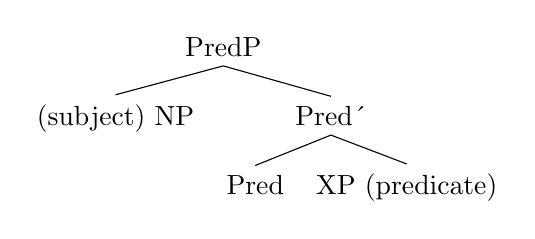
\begin{tikzpicture}[baseline=-0pt, remember picture]
\tikzset{level distance=25pt, sibling distance=5pt}
\Tree [.PredP {(subject) NP} [.Pred´ Pred {XP (predicate)} ]]]]
\end{tikzpicture}

There are many syntactic points of justification and empirical arguments why the category \textsc{pred} is necessary, and why, besides its semantic dimension, it should be kept apart from VP. These include the following (see especially \citealt[598–599]{bowers:1993:predication}):\footnote{As with regard to the syntactic head \textsc{mod}, the adoption of a universal head \textsc{pred} is not without controversy. For discussion see \citet{bowers:1993:predication, bowers:2002:pred, svenonius:1996:pred, dikken:2006:relators, heycock:2013:syntax} as well as \citet{matushansky:2019:against} and \citet{bruening:2020:category}, who have spoken decisively against this hypothesis. Besides theory-internal problems, the authors argue that the relevant head is redundant, as many problems it meant to solve in the original theory can now be solved via other mechanisms, and this is indeed the case. For instance, unlike categories can also be coordinated via a Boolian phrase.

\par

Furthermore, \citet{matushansky:2019:against} tries to show that the alleged manifestations of \textsc{pred} in several languages do not hold, because each language shows exceptions, where a copular element does not appear even though one would expect it to. In Edo, the alleged \textsc{pred} elements do not appear in resultatives, in Welsh they do not appear in PPs, in the Berber language East Riffian they are restricted to adjectives of Arabic origin \citep[sec. 4]{matushansky:2019:against}.

\par

While this is problematic for the universality of the Pred-hypothesis, Matushansky's analysis does not prove that no \textsc{pred}-like elements exist. What holds for \textsc{mod} also holds for \textsc{pred}: The relevant element is attested in Japanese and sticking with the idea of language-uniformity, I acknowledges its value and argue that it is present in Japanese and by extension cross-linguistically.}

\ex. Having a functional head \textsc{pred} allows for the coordination of unlike lexical categories.

\citet{bowers:1993:predication} explained cases such as \textit{I regard him [[\textsubscript{DP} a fool] and [\textsubscript{AP} unable to do his job.]]} without having to resort to non-binary structures. Both coordinates are being mediated by the predication head. %\is{predicative copula}

\ex. It enables movement of lexical categories, with the possibility that the subject can remain in Spec, PredP.

In a sentence such as \textit{How stupid do [\textsubscript{PREDP} I [\textsubscript{PRED} consider him?]]}, the subject remains in-situ, while phrasal material moves above it. This was a significant contribution at the time (cf. \citealt[68–69]{matushansky:2019:against} for discussion).

\ex. PredP provides a syntactic position for the subject in expletive-construction and various other small clauses, fulfilling the EPP even in absence of thematic relations.

Exemplifying with tenseless small clauses such as \textit{I consider [him stupid.]}, no obvious subject position is available. This subject position is, however, offered by \textsc{pred} in addition to licensing predication.

\ex. Subject and object position are kept apart, the subject being in Spec, PredP, the object in Spec, VP.

This relates to the previous point in the sense that also non-thematic subjects, for example those in \textit{tough} constructions, receive a subject position, although this position is not related to thematic role assignment, i.e. that of the agent.

\ex. Many languages have overt realizations of \textsc{pred}.

Probably the strongest piece of evidence for \textsc{pred} is offered by its lexical and syntactic manifestations in various languages. This includes \textit{as} and \textit{for}, which appear in small clauses with matrix verbs such as \textit{regard} in absence of a copula in English \ref{predenglish} \citep[596]{bowers:1993:predication}. Similar analyses have been proposed for the cross-linguistic counterparts of these elements, for example Russian \textit{kak} `as' \ref{predrussian} (or \textit{za} `as' or \textit{v} `in’; cf. \citet{bailyn:2002:overt}.\footnote{Further possible manifestations of \textsc{pred} include instrumental case in Russian \citep{bailyn:2001:syntax}, and copular elements in a variety of African languages including Edo and Chichiewa \citep{baker:2003:cat}, as well as Welsh \citep{bowers:2002:pred} and Greek \citep{campos:2004:ds}.}
%\is{predicative copula} %\is{English} %\is{Russian}

\ex. \ag. I regard [\textsubscript{SC}John as crazy].\\
\textsc{sub} \textsc{v} \textsc{obj} \textsc{pred} \textsc{a} \null\hfill \citep[596]{bowers:1993:predication} \label{predenglish}\\
\bg. On vygladit [kak durak]. (Russian)\\
he look \textsc{pred} fool\\
`He looks like a fool.’ \null\hfill \citep[39]{bailyn:2002:overt} \label{predrussian}

This also includes the overt manifestations of \textsc{pred} in Japanese. Besides depictives, presented in \ref{overtpred}, another instance where the predicative copula is manifested in absence of the dummy copula are coordination structures. As argued in Chapter \ref{coordination copula}, \textsc{de} must either autonomously or together with the sentential conjunction marker \textsc{katsu} establish coordination of two nominals. Such examples were analyzed as clausal coordination in which two instances of the copula must appear, one at the end of the sentence as the main clause predicate, one after the first conjunct. An example is repeated below (cf. \citealt[364]{hiraiwa:2012:mechanism}, from which examples are adapted). %\is{predicative copula} %\is{coordination}

\exg. Kono hito-wa Ken-no sensei *(katsu) / *(de) Naomi-no sensei-da.\\
this person-\textsc{top} Ken-\textsc{mod} teacher and / \textsc{pred} Naomi-\textsc{mod} teacher-\textsc{cop}\\
`This person is Ken's teacher and Naomi's teacher.’

Recall also that direct modifiers, such as \textit{Chūgoku-no} `Chinese’, on the other hand, can never appear in such coordination structures, not even as the second modifier in the DP. As they can never co-occur with the copula in predicative position, it is expected that they can therefore never co-occur with \textsc{de} either, if this element has copular status as well.

\ex. \ag. *Chūgoku-de kirei-na kabin\\
China-\textsc{pred} pretty-na vase\\
\bg. *kirei-de Chūgoku-no 	kabin\\
beautiful-\textsc{pred} China-\textsc{mod} vase\\
(`a Chinese and beautiful vase’)

Finally, there are some historical pieces of evidence for the copular status of \textsc{de}. This form in fact goes back to an amalgamation of the premodern copula \textsc{ni} -- the short form of the premodern copula inflected for nominalization form \textit{nari} -- and the coordinative suffix \textsc{te}. These two elements began in Classical Japanese to phonologically assimilate and have completed merging into one element, \textsc{de}, in Modern Japanese \citep{frellesvig:2010:history, miyama:2011:da}. %\is{predicative copula} %\is{Classical Japanese}

This means that /de/ in \textsc{de-ar-u} and in \textsc{de-at-ta} is the predicative copula. The representation of all three elements thus looks as follows.

\newpage

\ex. \ag. Yoru-ga shizuka-de-ar-u.\\
night-\textsc{nom} quiet-\textsc{pred-cop-prs}\\
`The night is quiet.'
\bg. Yoru-ga shizuka-de-at-ta.\\
night-\textsc{nom} quiet-\textsc{pred-cop-pst}\\
`The night was quiet.' \null \hfill \citep[189, 194]{nishiyama:1999:adj}

What about /d/ in \textsc{d-at-ta}, in which the vowel /e/ is not present? The vowel /e/ is deleted here \citep[203]{nishiyama:1999:adj}, probably to avoid the clashing of two vowels, a phenomenon not uncommon in Japanese, both diachronically and synchronically. %\is{predicative copula}

Coming now to \textit{i}-adjectives, those exhibit, in certain contexts, the same complex tripartite of morphemes parallel to the complex form \textsc{de-ar-u}. This complex form is \textsc{ku-ar-u}. It is straightforward, and the analysis adopted in \citet{nishiyama:1999:adj}, that \textsc{ku} corresponds to \textsc{de}. All things being equal, these two complex forms only differ in one aspect, namely the realization of the predicative copula. Japanese thus provides evidence for a second possible realization of \textsc{pred}.

One thing to consider is that \textsc{ku-ar-u} is restricted in its distribution and rather marked in canonical root clauses. %\is{emphatic expressions}

\exg. ??Ano doresu-wa taka-ku-ar-u.\\
that dress-\textsc{top} expensive-\textsc{pred-cop-prs}\\
`That dress is expensive.'

A prominent context in which this complex form is allowed, however, are emphatic expressions containing the focus-sensitive particles \textsc{mo} `even', \textsc{sae} `even' or \textsc{bakari} `only’. Interestingly, those intervene between \textsc{ku} and \textsc{ar-u}.\footnote{This was noted as early as \citet{miyata:1948:nihongo}, see \citet[185]{nishiyama:1999:adj} and \citet{kubo:1992:japanese}. It is unclear where exactly those focus markers emerge and are situated.}

\exg. Ano doresu-wa taka-ku mo ar-u.\\
that dress-\textsc{top} expensive-\textsc{pred} \textsc{emp} \textsc{cop-prs}\\
`That dress is even expensive.'

There are further instances where \textit{i}-adjectives must co-occur with these morphological complex forms: Before the modals \textit{beki} `should’ and \textit{mai} `will not be’ and in subordinate clauses with the complementizer \textit{koto} (\citealt[199]{nishiyama:1999:adj} and \citealt[51]{miyama:2011:da}). In these cases, these elements form a direct string. %\is{predicative copula}

%\newpage

\ex. \ag. Ano doresu-wa taka-ku-ar-u beki-da / mai.\\
that dress-\textsc{top} expensive-\textsc{pred-cop-prs} should-\textsc{cop} / will.not.be\\
`That dress should be / will not be expensive.'
\bg. Ano doresu-wa taka-ku-ar-u koto-wo wasure-ta.\\
that dress-\textsc{top} expensive-\textsc{pred-cop-prs} \textsc{comp}-\textsc{acc} forget-\textsc{pst}\\
`I forgot that that dress is expensive.'

In the same constructions, \textit{na}-adjectives (and \textit{no}-modifiers) must co-occur with the corresponding form of the canonical copula \textsc{de-ar-u}  (or past \textsc{de-at-ta}), in fact \textsc{da} is not possible \citep[186]{nishiyama:1999:adj}. As shown in \ref{shikkudemo}, their use in emphatic contexts further highlights the parallelism between \textsc{k(u)} and \textsc{de}. %\is{predicative copula}

\exg. Ano doresu-wa shikku-de-ar-u beki-da / *shikku-da beki-da.\\
that dress-\textsc{top} chic-\textsc{pred-cop-prs} should-\textsc{cop} / chic-\textsc{cop} should-\textsc{cop}\\
`That dress should be chic.'

\exg. Ano doresu-wa shikku-de mo ar-u.\\
that dress-\textsc{top} chic-\textsc{pred} \textsc{emp} \textsc{cop-prs}\\
`That dress is even chic.' \label{shikkudemo}

\textsc{k(u)} also appears in other contexts in which \textsc{de} appears, for instance in coordinative structures involving \textit{i}-adjectives. Recall from Chapter \ref{coordination copula} that it is optionally followed by -\textsc{te}, yielding the more canonical option. Now, we can safely identify \textsc{ku} in these contexts as the predicative copula as well.%\is{predicative copula} %\is{coordination}

\exg. aka-ku-(te) utsukushi-i doresu\\
red-\textsc{pred-ger} beautiful-\textsc{mod} dress\\
`a red and beautiful dress'

The predicative copula is used in tenseless constructions as well, for example in resultative, inchoative and causative constructions. As expected, it is not followed by the dummy copula in these contexts, because a verb is present to establish tense. This can be put forth as a further piece of evidence that Japanese has a requirement for \textsc{pred} (different to, for example, English, visible in the translations); for similar examples and discussion also see \citet[8–10]{yamada:2023:looking}. Finally, the adverbial inflectional form of \textit{i}-adjectives is also /ku/ and receives the same analysis as \textsc{pred} \citep{nishiyama:2005:baker}, but there is some controversy \citep{namai:2002:word}. %\is{predicative copula}

%\newpage

\ex. \ag. Jon-ga kabe-wo aka-ku nut-ta.\\
John-\textsc{nom} wall-\textsc{acc} red-\textsc{pred} paint-\textsc{pst}\\
`John painted the wall red.’ \\ \null\hfill resultative \citep[153]{nishiyama:2005:baker}
\bg. utsukushi-ku nar-u\\
beautiful-\textsc{pred} become-\textsc{prs}\\
`become beautiful' \null \hfill inchoative
\cg. utsukushi-ku sur-u\\
beautiful-\textsc{prs} do-\textsc{prs}\\
`make beautiful' \null \hfill causative
\dg. haya-ku arui-ta\\
fast-\textsc{pred} walk-\textsc{pst}\\
`walked fast' \null \hfill adverbial

Next we come to past contexts. Consider first the following example in which an \textit{i}-adjective is inflected for past and the morphological complex form is \textsc{ku-at-ta}. A focus sensitive particle occurs between the predicative and the dummy copula, as in the examples above.%\is{predicative copula}

\exg. Hanako-wa kanashi-ku sae at-ta.\\
Hanako-\textsc{top} sad-\textsc{pred} \textsc{emp} \textsc{cop-pst}\\
`Hanako was even sad.' \null\hfill \citep[109]{kubo:1992:japanese}

In past contexts, when the three elements occur uninterrupted, \textit{i}-adjectives co-occur with the complex form \textsc{k-at-ta}, not \textsc{ku-at-ta}, as given below.

\exg. Ano doresu-wa taka-k-at-ta.\\
that dress-\textsc{top} expensive-\textsc{pred-cop-pst}\\
`That dress was expensive.'

We can conclude that \textsc{ku-at-ta}, or \textsc{k-at-ta}, contain the same elements as \textsc{de-at-ta}, or \textsc{d-at-ta}. However, there is no free alternation and \textsc{k-at-ta} has a default character. Instead of formalizing a parallel rule of contraction and vowel reduction, \citet[192–193]{nishiyama:1999:adj} treats [u] as an epenthetic vowel and simply analyzes the consonant part /k/ as \textsc{pred}. This analysis receives support from phonological observations. As Japanese favors open syllables, an epenthetic [u] is often inserted in word-final position as well \citep{kubozono:2005:rendaku, ito:2015:word}. The analysis also becomes relevant for the treatment of the simple element -\textsc{i} (see Chapter \ref{kitoi}) and will be adopted in the spell-out rule below. %\is{predicative copula}  %\is{predicative copula} %\is{negation}

Before closing this subsection, I point out two more scenarios in which the predicative copulas \textsc{de} and \textsc{k(u)} appear. One concerns negation. Given what we know about predication and its syntactic realization in Japanese, it is expected that the predicative copula has to appear in contexts of negation in order to license predication.

Negation is expressed via the negative element \textsc{na}, which can probably be regarded as the negative form of the dummy copula.\footnote{Since it inflects exactly like an \textit{i}-adjective, it is also often classified as such. Note that -\textsc{i}, as it appears in predicative position, will be analyzed as an amalgamation of copulas and tense markers following \textit{i}-adjectives below, and is therefore not glossed for now.} In the case of \textit{na}-adjectives, additionally the topic marker \textsc{wa} intervenes between this element and the predicative copula  \ref{negation na long}.\footnote{Note that \textsc{wa} could very well also be analyzed as a focus marker here, as done in \citet[6]{yamada:2023:looking}, but nothing hinges on this.} In colloquial speech, \textsc{de} and \textsc{wa} are contracted to \textsc{ja} \ref{negation na short}.\footnote{The predicative copula is also obligatory for the polite form of negation, in which the existential verb, i.e. the dummy copula \textsc{ar}, is followed by the polite auxiliary element -\textsc{mas}-. %\is{negation}

\par

\exg. Ano doresu-wa shikku-de-wa-ari-mase-n.\\
that dress-\textsc{top} chic-\textsc{pred-top-cop-aux.pol-neg}\\
`That dress is not chic.'

\par

}

%\newpage

\exg. Ano doresu-wa utsukushi-ku-nai.\\
that dress-\textsc{top} beautiful-\textsc{pred-neg}\\
`That dress is not beautiful.' \null \hfill negation, \textit{i}-adjective \label{negation i}

\ex. \ag.  Ano doresu-wa shikku-de-wa-nai.\\
that dress-\textsc{top} chic-\textsc{pred-top-neg} \label{negation na long}\\
\bg. Ano doresu-wa shikku-ja-nai.\\
that dress-\textsc{top} chic-\textsc{pred.top-neg}\\
`That dress is not chic.' \null \hfill negation, \textit{na}-adjective \label{negation na short}

On a final note, \textsc{pred} has another realization, namely /ni/, as argued in \citet{nishiyama:1999:adj}. This element co-occurs with \textit{na}-adjectives in tenseless environments, such as resultative, inchoative and causative constructions, but not in depictives. Under such an analysis, it can be given the same status as \textsc{k(u)}, meaning that \textit{na}-adjectives show an alternation in the realization of \textsc{pred} that \textit{i}-adjectives do not show (\citealt[205–208]{nishiyama:1999:adj}).\footnote{Again, I present Nishiyama’s analysis of adverbially used \textit{na}-adjectives as co-occurring with \textsc{pred} at face value without comments, knowing there is yet to be found empirical proof for these claims. An alternative could be to treat \textsc{ni} as an instance of the homophonous dative marker as suggested to me by Jim Kotopoulis.}

\ex. \ag. Jon-ga kabe-wo makka-ni nut-ta.\\
John-\textsc{nom} wall-\textsc{acc} crimson.red-\textsc{pred} paint-\textsc{pst}\\
`John painted the wall crimson red.’ \\ \null\hfill resultative \citep[207]{nishiyama:1999:adj}
\bg. shizuka-ni nar-u\\
quiet-\textsc{pred} become-\textsc{prs}\\
`become quiet' \null \hfill inchoative
\cg. shizuka-ni sur-u\\
quiet-\textsc{pred} do-\textsc{prs}\\
`make quiet' \null \hfill causative
\dg. shizuka-ni arui-ta\\
quiet-\textsc{pred} walk-\textsc{pst}\\
`walked quietly' \null\hfill adverbial \citep[150]{nishiyama:2005:baker}

To summarize, Japanese provides lexical evidence for the head \textsc{pred}, which is conditioned in its realization by word class, syntactic environment and phonology. I propose the following spell-out rules adopted from \citet[207]{nishiyama:1999:adj}, where [+V] represents resultative, inchoative and causative use of \textit{na}-adjectives respectively. These rules mean that \textsc{pred} is always realized as /k/ when preceded by an \textit{i}-adjective, as /ni/ when preceded by a \textit{na}-adjective in a tensed environment and otherwise as /de/.

\ex. Spell-out rule for \textsc{pred} in Japanese\\
$[Pred]$\phantom{; +V} $\leftrightarrow$ /k/ / iA \_ \\
$[Pred; +V]$ $\leftrightarrow$ /ni/ / naA \_ \\
\phantom{$[Pred; +V]$ $\leftrightarrow$} /de/

\subsubsection{Structural representation of predicative use}

Having established the ingredients of the morphologically complex forms \textsc{de-at-ta}/\textsc{d-at-ta}, \textsc{de-ar-u} and \textsc{k-at-ta}, I will now derive the relevant structure, which I adopt from \citet[189–194]{nishiyama:1999:adj}. I will start with the predicative structure for past.

\ex. Predicative \textit{na}-adjectives in past \null\hfill \citep[189, 194]{nishiyama:1999:adj}
\ag. Yoru-ga shizuka-d(e)-at-ta.\\
night-\textsc{nom} quiet-\textsc{pred-cop-pst}\\
`The night was quiet.'
\b. \begin{tikzpicture}[baseline=-0pt]
\tikzset{level distance=25pt, sibling distance=5pt}
\Tree [.TP [.NP \edge[roof]; {yoru} ] [.T´ [.CopP [.PredP [.AP \edge[roof]; {shizuka} ] [.Pred {de} ] ] [.Cop {ar} ]] [.T {ta} ]]]
\end{tikzpicture}

\ex. Predicative \textit{i}-adjectives in past \null\hfill \citep[190, 192]{nishiyama:1999:adj}
\ag. Doresu-ga utsukushi-k-at-ta.\\
dress-\textsc{nom} beautiful-\textsc{pred-cop-pst}\\
`The dress was beautiful.'
\b. \begin{tikzpicture}[baseline=-0pt]
\tikzset{level distance=25pt, sibling distance=5pt}
\Tree [.TP [.NP \edge[roof]; {doresu} ] [.T´ [.CopP [.PredP [.AP \edge[roof]; {utsukushi} ] [.Pred {ku} ] ] [.Cop {ar} ]] [.T {ta} ]]]
\end{tikzpicture}

These structures are exactly parallel, the only difference being the different spell-out of \textsc{pred}. The structure for non-past \textsc{de-ar-u} is also exactly analogous, mind the different tense marker for non-past.

%\newpage

\ex. Predicative \textit{na}-adjectives in non-past \null\hfill \citep[189, 194]{nishiyama:1999:adj}
\ag. Yoru-ga shizuka-de-ar-u.\\
night-\textsc{nom} quiet-\textsc{pred-cop-prs}\\
`The night is quiet.'
\b. \begin{tikzpicture}[baseline=-0pt]
\tikzset{level distance=25pt, sibling distance=5pt}
\Tree [.TP [.NP \edge[roof]; {yoru} ] [.T´ [.CopP [.PredP [.AP \edge[roof]; {shizuka} ] [.Pred {de} ] ] [.Cop {ar} ]] [.T {u} ]]]
\end{tikzpicture}

\subsection{Application to attributive use}

As the past forms \textsc{k-at-ta} and \textsc{d(e)-at-ta} as well as the non-past form \textsc{de-ar-u} can be used attributively without morphological difference to their predicative counterparts, the predicative structure can simply be translated into an attributive structure. According to Nishiyama, attributively used adjectives project an additional CP layer whose head is empty and contains a relative clause feature (\citealt[197]{nishiyama:1999:adj}; cf. \citealt{kaplan:1995:the}). In the tree below, I depict the structure for a DP containing a \textit{na}-adjective inflected for past. The structures for \textsc{k-at-ta} and \textsc{de-ar-u} are analogous apart from the different realization forms of \textsc{pred} and I.

%\newpage

\ex. Attributive \textit{na}-adjectives in past \null\hfill \citep[197]{nishiyama:1999:adj}
\ag. shizuka-d(e)-at-ta yoru\\
quiet-\textsc{pred-cop-prs} night\\
`the night which was quiet'
\b. \begin{tikzpicture}[baseline=-0pt]
\tikzset{level distance=25pt, sibling distance=5pt}
\Tree [.NP [.CP [.TP [.CopP [.PredP [.AP \edge[roof]; {shizuka} ] [.Pred {de} ] ] [.Cop {ar} ] ] [.T {ta} ] ] [.C {[RC]} ] ] [.NP \edge[roof]; {yoru} ] ]
\end{tikzpicture}

\subsection{Application to predicative \textit{da} and \textit{i}} \label{kitoi}

Next, the analysis can be extended to the predicative elements \textsc{da} and \textsc{i}.

\subsubsection{Predicative \textit{da}}

It is a standard assumption that \textsc{da} is a variant of the canonical copula \textsc{de-ar-u} \citep{urushibara:1993:syntactic} and these elements have been treated similarly in this book. There are several pieces of evidence for this claim (cf. \citealt{miyama:2011:da}). First, those elements are almost equally distributed, and they are mutually exclusive. However, while \textsc{de-ar-u} can appear in almost all environments (except before sentence-final particles where it is marked, \citealt[45–46]{miyama:2011:da}), \textsc{da} cannot. Instances where it is not possible include attributive structures, and, as mentioned above, before certain grammatical elements such as \textit{beki} `should’, as well as in emphatic constructions. Second, that \textsc{da} is likely historically derived from \textsc{de-ar-u} is suggested by the in-between stages \textsc{de-ar} and \textsc{dea} \citep{nakahara:2002:japanese}. %\is{predicative copula} %\is{Classical Japanese}

From a morphosyntactic perspective, a corresponding analysis of \textsc{da} to \textsc{de-ar-u} seems to be pretty straightforward as well -- at least to a certain point. Morphologically, the initial consonant /d/ can receive an analysis as \textsc{pred}, exactly parallel to /d/ in \textsc{d-at-ta}. The vowel /a/ is a realization of the dummy copula \textsc{cop}. %\is{dummy copula}

It is crucial to note that /da/ cannot be an allomorph of /de/, since the two forms are not paraphrasable, not even in emphatic constructions. Compare \ref{danotde} to \ref{shikkudemo}. %\is{emphatic constructions}

\exg. *shizuka-da mo ar-u\\
quiet-\textsc{da} \textsc{emp} \textsc{cop-prs}\\
(`it is even quiet’) \null \hfill \citep[186]{nishiyama:1999:adj} \label{danotde}

What is striking is the alleged absence of a tense marker. Based on the fact that \textsc{da} and \textsc{de-ar-u} are, in most environments, interchangeable, Nishiyama simply treats the two as allomorphs and assumes that all three elements -- predicative copula, dummy copula and tense marker for non-past -- are simply combined in /da/ as shown below \citep[196–197]{nishiyama:1999:adj}.

\exg. Yoru-ga shizuka-da.\\
night-\textsc{nom} quiet-\textsc{pred.cop.prs}\\
`The night is quiet.' \null \hfill (Nishiyama's analysis)

Nothing immediately hinges on this, but I will assume here that the predicative copula is the consonant /d/ and that the dummy copula and the tense marker for present are merged in /a/ as shown below.

\ex. \textsc{d-a} = \textsc{pred-cop.prs}

This means that \textsc{da} is not derived from \textsc{de-ar-u}, but simply a shorter form, in which all relevant elements, including the tense marker, are still present.

\subsubsection{Predicative \textit{i}} \label{predicativei}

A similar structure can be derived for \textit{i}-adjectives, although predicative -\textsc{i}, at first glance, does not seem to bear any resemblance to \textsc{ku-ar-u}. First, note that non-past is the only environment in which the velar consonant /k/ is absent in the inflectional paradigm of \textit{i}-adjectives. In Classical Japanese, however, the attributive form of the inflectional paradigm of \textit{i}-adjectives was -\textsc{ki}, thus included this consonant (cf. \citealt[189–190]{nishiyama:1999:adj}). \citet{nishiyama:1999:adj} accounts for these facts as follows: Modern \textsc{i} is a direct successor of \textsc{ki} derived via a historical devoicing process (cf. \citealt{frellesvig:2010:history}). The consonant /k/ was an instance of \textsc{pred} and continued this role in Modern Japanese, although it is not pronounced. He formalizes this through a \textit{Velar-filter} \citep[191]{nishiyama:1999:adj}. %\is{predicative copula}

In other words, the head of PredP is structurally present, but phonologically reduced.\footnote{Such phonological processes are not uncommon diachronically, as the consonant /k/ has been systematically reduced in front of the vowel /i/ \citep[340]{frellesvig:2010:history}, but also attested synchronically with certain verb forms. For example, the past form of \textit{kak} `to write' is \textit{kai-ta}, not *\textit{kaki-ta} \citep[191]{nishiyama:1999:adj}.} \textit{i}-adjectives thus co-occur with the underlying elements \textsc{\st{k}-i}, which constitute a combination of the predicative copula and a tense marker and are realized as /i/ (cf. \citealt[199–201]{nishiyama:1999:adj}; cf. also \citealt[2]{baker:2003:verbal}).

\ex. Nishiyama's analysis for \textit{i}-adjectives in non-past
\ag. Ano doresu-ga taka-\st{k}-i.\\
that dress-\textsc{nom} expensive-\textsc{pred-prs}\\
`That dress is expensive.'

But, under this analysis no dummy copula is present. Recall that this is also the case in other languages in default non-past contexts for instance Hebrew \citep{doron:1983:verbless, rapoport:1987:copular} and Russian \citep{babby:2010:syntactic}, as in the example in \ref{pagoda} repeated below. This can thus be applied to Japanese (\citealt[191–192]{nishiyama:1999:adj}, and see \citealt{urushibara:1993:syntactic}). %\is{copula} %\is{Russian}

\exg. Pagoda xorošaja.\\
weather.\textsc{nom.sg.f} good.\textsc{nom.sg.f}\\
`The weather is good.' \null \hfill Russian

An obvious challenge to this account is the question how tense is supported, if no dummy copula is present. As explained above, the dummy copula is needed to support the I node and establishes some kind of \textit{be}-support. And while no overt tense is present in the Russian example, Nishiyama argues that non-past information is included in \textsc{i}. Furthermore, how can the parametric difference between \textit{i}- and \textit{na}-adjectives, that necessarily arises, be accounted for? For lack of better alternative, I assume for predicative \textsc{i} almost the same structure as for \textsc{da}: The predicative copula is represented via the filtered consonant /k/, and the dummy copula and the tense morpheme are merged in /i/. %\is{velar filter} %\is{Classical Japanese}

\ex. \textsc{(k)-i} = \textsc{pred-cop.prs}

\subsection{Why the application to attributive \textit{i} and \textit{na} fails} \label{why it fails}

This section refutes Nishiyama's analysis of the attributive forms for non-past, \textsc{i} and \textsc{na}, as copular elements. It is not surprising that \citet{nishiyama:1999:adj} puts forth the same analysis for \textsc{i} in attributive contexts as for \textsc{i} in predicative contexts, thus treats those as the same elements. The only difference is that, the adjective projects an additional CP layer. He suggests the following \citep[199–202]{nishiyama:1999:adj}. %\is{velar filter}

\ex. Attributive \textit{i}-adjectives in non-past according to Nishiyama (not correct)
\ag. taka-(k-)i doresu\\
expensive-\textsc{pred-prs} dress\\
`dress which is expensive'\\
\b. \begin{tikzpicture}[baseline=-0pt]
\tikzset{level distance=25pt, sibling distance=5pt}
\Tree [.NP [.CP [.TP [.PredP [.AP \edge[roof]; {taka} ] [.Pred {\st{k}} ] ] [.T {i} ] ] [.C {[RC]} ] ] [.NP \edge[roof]; {doresu} ] ]
\end{tikzpicture}

For \textit{na}-adjectives, \citet[196–199]{nishiyama:1999:adj} analyzes \textsc{na} as the very same element as \textsc{da}, thus as a combination of predicative copula, dummy copula and tense marker for non-past. The only difference in consonant realization is conditioned by the presence of a CP. This means that the labor between predicative and attributive use is strictly divided in \textit{na}-adjectives via \textsc{da} and \textsc{na}, which are allomorphs and not interchangeable \citep[197]{nishiyama:1999:adj}. He gives the following phonological transformation rule in the spirit of Distributed Morphology \citep{halle:1993:distributed, halle:1994:some}.

\ex. [pred.cop, dum.cop, -past, rel.cl] $\leftrightarrow$ /na/ / NA \_ \\ \null \hfill \citep[197]{nishiyama:1999:adj}

\citet{nishiyama:1999:adj} treats all attributive adjectives in Japanese as embedded in a CP layer and therefore as indirect modifiers.\footnote{Nishiyama himself does consider the possibility of direct modification. He states ``[...] we know that natural language allows adjectives to act as direct modifiers (as in English). Thus, unless there is evidence to the contrary, the null hypothesis is that Japanese adjectives also act as direct modifiers [...]” \citep[201]{nishiyama:1999:adj} and mentions \textsc{mod} presented in Chapter \ref{internalstructure} as an alternative.} \citet{baker:2003:verbal} and \citet{hoshi:2002:kaynean} adopt his analysis and explicitly deny the possibility of direct modification in Japanese.

Nishiyama not only encourages the long-existing analysis of \textsc{na} as the attributive form of the copula, \citep{teramura:1982:nihongo, miyagawa:1987:lexical, murasugi:1991:noun, kubo:1992:japanese, urushibara:1993:syntactic}, but also manages to unify \textit{i}- and \textit{na}-adjectives by analyzing \textsc{i} in a parallel fashion. This is a significant contribution. However, this analysis overgeneralizes as presented in abundance throughout this book. Although sometimes up for discussion, the last chapter mentioned many direct \textit{i}- and \textit{na}-adjectives such as the following, and see especially \citet{yamakido:2005:nature} or \citet{ayano:2010:revisiting} from where these examples are repeated. %\is{direct modifiers}

\ex. \ag. Omoigakena-i kyaku-ga ki-ta.\\
unexpected-\textsc{mod} guest-\textsc{nom} come-\textsc{pst}\\
`An unexpected guest came.' \null \hfill \citep[67]{yamakido:2005:nature}
\bg. *Ano kyaku-ga omoigakena-i.\\
that guest-\textsc{nom} unexpected-\textsc{pred.cop.prs}\\
(`That guest is unexpected.’)

\ex. \ag. Max-ga kanzen-na baka-d-a.\\
Max-\textsc{nom} complete-\textsc{mod} idiot-\textsc{pred-cop.prs}\\
`Max is a complete idiot.' \null \hfill \citep[68]{yamakido:2005:nature}
\bg. *Ano baka-ga kanzen-d-a.\\
that idiot-\textsc{nom} complete-\textsc{pred-cop.prs}\\
(`That idiot is complete.’)

This means \textsc{i} and \textsc{na} in attributive position cannot be universally analyzed as copular elements which is why I deny this analysis in favor of \textsc{mod} (Chapter \ref{internalstructure}). In turn, this means there are two different instances of \textsc{i}: A copular element in predicative position and the syntactic linker \textsc{mod} in attributive position.

\subsection{Application to \textit{no}-modifiers}

The analysis presented here can be straightforwardly extended to \textit{no}-modifiers, which share their entire inflectional paradigm with \textit{na}-adjectives with the exception of \textsc{no}. All the elements receive the same analysis, illustrated first with \textsc{da} and \textsc{de-ar-u} in combination with a clear noun \ref{clear noun}, and a more adjectival \textit{no}-modifier (\textit{no}-adjective, \ref{noadjective}). See also \citet[195]{nishiyama:1999:adj}. %\is{no-modifiers}

\ex. \label{clear noun} \ag. Hanako-wa sensei-d-a.\\
Hanako-\textsc{top} teacher-\textsc{pred-cop.prs}\\
\bg. Hanako-wa sensei-de-ar-u.\\
Hanako-\textsc{top} teacher-\textsc{pred-cop-prs}\\
`Hanako is a teacher.' \null \hfill noun

\ex. \label{noadjective} \ag. Haishīzun-ni-wa hayame-no yoyaku-ga hisshu-d-a.\\
high.season-\textsc{loc-top} early-\textsc{mod} reservation-\textsc{nom} necessary-\textsc{pred-cop.prs}\\
\bg. Haishīzun-ni-wa hayame-no yoyaku-ga hisshu-de-ar-u.\\
high.season-\textsc{loc-top} early-\textsc{mod} reservation-\textsc{nom} necessary-\textsc{pred-cop-prs}\\
`During high season, early reservation is necessary.’\footnote{ISHIMORI Hiromi: \textit{Tabi, chotto senchimentaru}. Tankobon, 2002. Retrieved via BCCWJ.} \\ \null \hfill \textit{no}-adjective

The analysis also carries over to \textsc{de-at-ta}, which can-occur with a \textit{no}-modifier as well.

\exg. Hanako-wa sensei-de-at-ta.\\
Hanako-\textsc{top} teacher-\textsc{pred-cop-pst}\\
`Hanako was a teacher.' \null \hfill noun, past

Naturally, this extends to the attributive use of \textsc{de-ar-u} and \textsc{de-at-ta}. Same as \textsc{da} and \textsc{de-ar-u} are mutually exclusive in predicative position, \textsc{no} and \textsc{de-ar-u} are mutually exclusive in attributive position.

%\newpage

\exg. sensei-de-ar-u Hanako\\
teacher-\textsc{pred-cop-prs} Hanako\\
`Hanako, who is a teacher'

Although Nishiyama does not focus on \textsc{no}-modifiers, he proposes a spell-out rule for \textit{no} as well, which looks as follows.

\ex. [pred.cop, dum.cop, -past, rel.cl] $\leftrightarrow$ /no/ \_ \\ \null \hfill (Nishiyama’s analysis of \textsc{no}; \citealt[197]{nishiyama:1999:adj})

This spell-out rule says that \textsc{no} is a manifestation of the predicative copula, dummy copula and non-past tense marker and appears in relative clause contexts. It is realized in the elsewhere-case, meaning when the modifier is not a clear \textit{na}-adjective.

As in the case of the other modifiers, this cannot be the right analysis given the abundance of direct modifiers among the group of \textit{no}-modifiers. Instead, I have put forth an analysis in Chapter \ref{internalstructure} of \textsc{no} as an instance of \textsc{mod} which is blocked when \textsc{de-ar-u} or other elements with an overt I-head appear.

However, it is worth emphasizing that the existence of such cases, those in which a \textit{no}-modifier has a clear predicative function, show that not all \textit{no}-modifiers are direct. This, in turn, refutes a claim made in \citet{nagano:2015:RA}, who argue, ``Japanese adjectives differ from English adjectives in formally disambiguating direct and indirect modification'' \citep[124]{nagano:2015:RA}. According to the authors, it is only \textit{no}-modifiers which are responsible for direct modification, all other modifiers in Japanese being indirect. However, this is simply not true as shown in many examples throughout this book and in the data set. %\is{no-modifiers}

\subsection{The integration of indirect modifiers into the DP}

The complex morphological elements deduced in this section can be neatly integrated along the modifier into a cartographic structure of the DP. This is exemplified below with a \textit{na}-adjective inflected for past, but the derivation is exactly parallel for the other elements for past (\textsc{d-at-ta} for \textit{no}-modifiers, \textsc{k-at-ta} for \textit{i}-adjectives) as well as \textsc{de-ar-u} for non-past. Indirect modifiers are merged in a functional projection in the indirect domain and are embedded in a complex set of functional layers whose heads spell-out the predicative copula, the canonical copula and the tense morpheme respectively.\footnote{In this chapter, I will not include the universal syntactic head \textsc{mod} in the visualizations of relative clauses in cases where it is not realized. The CP status of relative clauses will be defended in the following.}

\newpage

\ex. \ag. ano shizuka-d(e)-at-ta yoru \\
that quiet-\textsc{pred-cop-pst} night\\
`that night which was quiet'\\
\b. \begin{tikzpicture}[baseline=-0pt]
\tikzset{level distance=25pt, sibling distance=5pt}
\Tree [.DP\textsubscript{internal} ano [.D´\textsubscript{internal} [.FP\textsubscript{indirect} [.CP {} [.C´ [.IP {} [.I´ [.CopP {} [.Cop´ [.PredP {} [.Pred´ [.AP \edge[roof]; shizuka ] [.Pred de ] ] ] [.Cop ar ] ] ] [.I ta ] ] ] C ]] [.F´\textsubscript{indirect} [.... [.NP \edge[roof]; yoru ] {} ] F ] ] D ]]
\end{tikzpicture}

\subsection{A note on the polite elements} \label{desu}

At this point, the question remains why the polite copula \textsc{desu}, glossed as \textsc{cop.pol} up to now, and its counterpart for past \textsc{deshita} are mutually exclusive with the copular forms \textsc{de-ar-u} and \textsc{de-at-ta}, but follow \textsc{i} and also \textsc{k-at-ta}.\footnote{Assuming there are three stages of politeness in Japanese \citep{minami.1977:gendai}, \textsc{desu} expresses the medial level and is used when talking to strangers and superiors. In the verbal domain, the corresponding politeness is achieved via the polite auxiliary -\textsc{mas}-, in past \textsc{mashi-ta}. Also note that some other grammatical elements, for example the epistemic suffix \textit{mitai} `seem’, occur after \textsc{i} but replace \textsc{da} \citep{kubo:1992:japanese, urushibara:1993:syntactic, nishiyama:1999:adj}.} Observe some relevant examples. %\is{polite copula}

\ex. \ag. Ano doresu-wa shikku (*d-a) desu.\\
that dress-\textsc{top} chic \textsc{pred-cop.prs} \textsc{desu}\\
`That dress is chic.' \null \hfill polite non-past, \textit{na}-adjective
 \bg. Ano doresu-wa shikku (*d-at-ta) deshi-ta.\\
that dress-\textsc{top} chic \textsc{pred-cop-pst} \textsc{desu}-\textsc{pst}\\
`That dress was chic.' \null \hfill polite past, \textit{na}-adjective

\newpage

\ex. \ag. Ano doresu-wa taka-*(i) desu.\\
that dress-\textsc{top} expensive-\textsc{pred.cop.prs} \textsc{desu}\\
`That dress is expensive.' \null \hfill polite non-past, \textit{i}-adjective
\bg. Ano doresu-wa taka-k-at-ta desu.\\
that dress-\textsc{top} expensive-\textsc{pred-cop-pst} \textsc{desu}\\
`That dress was expensive.' \null \hfill polite past, \textit{i}-adjective \label{katta desu not deshita}

\ref{katta desu not deshita} is the only way to express politeness and past tense on an \textit{i}-adjective at the same time. The polite past form \textsc{deshita} never co-occurs with \textit{i}-adjectives.

\exg. *Ano doresu-wa taka-i deshi-ta.\\
that dress-\textsc{top} expensive-\textsc{pred.cop.prs} \textsc{desu}-\textsc{pst}\\
(`That dress was expensive.’) (polite)

In a recent analysis, \citet{yamada:2023:looking}, and see also \citet{miyagawa:2022:syntax}, argues that Modern Japanese has two separate instances of \textsc{desu}, which correspond to two different grammars. This explains the different distribution. In a nutshell, the element \textsc{desu} following \textit{na}-adjectives (and nouns/\textit{no}-modifiers) consist of the familiar tripartite of elements. The element \textsc{desu} following \textit{i}-adjectives, on the other hand, is just a single marker of politeness and crucially follows the copula \citep[2–4]{yamada:2023:looking}. %\is{polite copula} %\is{politeness}

In the first case, \textsc{desu/deshita} consist of the identical elements as \textsc{de-ar-u/de-at-ta}, but significantly, politeness is marked.Translated into the analysis proposed here, I treat -\textsc{u} and -\textsc{ta} as tense morphemes, \textsc{de} as the predicative copula, and the medial elements -\textsc{s}- and -\textsc{shi}- as the polite version of the dummy copula.\footnote{Note that the difference in consonant quality between the consonants /s/ and /sh/ is simply phonologically governed (see \citealt{ito:2015:word}). The epenthetic vowel [i] has to be inserted after /s/, preserving this consonant as well as the CV mora structure favored in Japanese. [i] becomes the coda of the new mora [\textctc i] (/shi/). The consonant shift of the preceding consonant from [s] to [\textctc] is systematic in the sense that the fricatives [s] and [z] always become alveolo-palatal before [i]. The mora [si] simply is never realized in Japanese \citep{lewin:1989:sprache, vance:2008:sounds}.} This means that the dummy copula is not simply semantically vacuous, but has a semantic and pragmatic dimension. Nevertheless it needs to support tense. Therefore, I maintain the gloss \textsc{cop.pol} for the medial part, highlighting that it is a polite version of the dummy copula, as shown below. %\is{politeness}

\ex. \ag. Yoru-ga shizuka-de-s-u.\\
night-\textsc{nom} quiet-\textsc{pred-cop.pol-prs}\\
`The night is quiet.' \null \hfill polite non-past, \textit{na}-adjective
\bg. Yoru-ga shizuka-de-shi-ta.\\
night-\textsc{nom} quiet-\textsc{pred-cop.pol-pst}\\
`The night was quiet.' \null \hfill polite past, \textit{na}-adjective

\textsc{desu} following \textit{i}-adjectives and their copular forms is a sort-of grammaticalized modal element and by itself projects the syntactic category \textsc{pol} (cf. \citealt[10–11]{yamada:2023:looking}). There is no need to express an additional dummy copula. I suggest the following structure.\footnote{I thank Ken Hiraiwa for suggesting and discussing these patterns with me. The analysis in \citet{yamada:2023:looking} is similar in that it proposes the emergence of a new grammar with a re-analysis of \textsc{desu} as a marker for addressee honorificity. Note that this politeness marker also follows the negative element \textsc{na}, which inflects like an \textit{i}-adjective.} %\is{politeness}

\exg. Ano doresu-wa taka-k-at-ta desu.\\
that dress-\textsc{top} expensive-\textsc{pred-cop-pst} \textsc{pol}\\
`That dress was expensive.' \null \hfill polite past, \textit{i}-adjective \label{katta desu}

There are some pieces of evidence for this claim. First, \textsc{desu} in \ref{katta desu} is syntactically not necessary, in contrast to its combination with \textit{na}-adjectives. This means it has a syntactic dummy status, albeit a more semantic contribution. Furthermore, \textsc{desu} in such instances is never paraphrasable with \textsc{de-ar-u} as shown below (and see \citealt[10–11]{yamada:2023:looking}).

\ex. \ag. *Ano doresu-wa taka-k-at-ta-de-ar-u.\\
that dress-\textsc{top} expensive-\textsc{pred-cop-pst-pred-cop-prs}\\
\bg. *sensei-de-wa-na-i-de-ar-u\\
teacher-\textsc{pred-top-neg-pred.cop.prs-pred-cop-prs}\\

Furthermore, use of the grammaticalized version of \textsc{desu} has in recent times increased. It is also attested after \textsc{d-at-ta}, where the copular elements are already present as well \citep{yamada:2023:looking}.

\exg. I-i mise d-at-ta desu.\\
good-\textsc{mod} restaurant \textsc{pred-cop-pst} \textsc{pol}\\
`It was a good restaurant.’ \null \hfill \citep[13]{yamada:2023:looking} \label{desudatta} %\is{politeness}

\citet{yamada:2023:looking} also gives examples where \textsc{desu} appears multiple times inside one sentence, each time followed by a sentence-final particle \ref{desufinal}.

\exg. Watashi-wa desu ne totemo desu ne tsukare-ta desu yo.\\
I-\textsc{top} \textsc{pol} \textsc{sfp} very \textsc{pol} \textsc{sfp} become.tired-\textsc{pst} \textsc{pol} \textsc{sfp}\\
`I (you know) got very (you know) tired (you know).’ \\ \null \hfill (\citealt[Fn. 34]{yamada:2023:looking}) \label{desufinal}

These examples show that this instance of \textsc{desu} has been grammaticalized into an element that simply marks politeness and co-occurs with the copula. To summarize:\footnote{Note that the question is left open why \textsc{desu} can never appear in attributive position.

\par

\exg. *ano shikku desu doresu\\
that chic \textsc{desu} dress\\
(`that chic dress’) (polite)

\par


Tentatively, I assume this really is a pragmatic ban, restricting politeness to the matrix clause. Some authors \citep{horie:2017:attributive} have shown that verbs in a polite speech style are in some instances possible in attributive position, especially then when the root verb is in the very polite speech style. Apparently, such constructions are common in the service domain.

\par

\exg. [O-mōshikomi-ni nari-mashi-ta] kādo-wo hakkō-sase-te-itadaki-mas-u.\\
\textsc{hon}-apply-\textsc{dat} become-\textsc{aux.pol-pst} card-\textsc{acc} issue-cause.\textsc{pol}-\textsc{ger}-humbly.receive-\textsc{aux.pol-prs}\\
`We shall respectfully issue a card [for which you had sent your application form].’ \\ \null \hfill \citep[51]{horie:2017:attributive}

\par


It is not necessary however to use the polite form of the verb in the embedded clause, and potentially this is a new trend to be as polite as possible that just has not reached the adjectival domain yet (Ken Hiraiwa p.c.).}

%\newpage

\ex.\a. \textsc{de-s-u} = \textsc{pred-cop.pol-prs} (\textit{na}-adjectives and nouns)
\b. \textsc{d(e)-shi-ta} = \textsc{pred-cop.pol-pst} (\textit{na}-adjectives and nouns)
\c. \textsc{desu} = \textsc{pol} (\textit{i}-adjectives and elsewhere)

To summarize, the element \textsc{de-s-u} is another form of the copula, and, as shown in the previous chapter, equally incompatible with direct modifiers. It contrasts with another element \textsc{desu} used to mark politeness.\footnote{The analysis of the element \textit{desu} as monostructural performed here is, in principle, consistent with the analysis given in \citet[64–67]{miyagawa:2022:syntax}. He analyzes this element as \textit{modal} and the head of a Mod(al)P, which, as is evident from the structural precedence, occurs higher than TP.

\par

Note that the analysis given here can be carried over to the epistemic element \textsc{d(e)arō}, which is, like \textsc{desu}, mutually exclusive with the copula \textsc{d-a}, but has to follow \textsc{i} and any tense morpheme when co-occurring with \textit{i}-adjectives and verbs respectively. Tentatively, I propose the following segmentation.

\par


\ex. \a. \textsc{d(e)-ar-ō} = \textsc{pred-cop-epis} (\textit{na}-adjectives and nouns)
\b. \textsc{d(e)arō} = \textsc{epis} (\textit{i}-adjectives and elsewhere)

\par

} %\is{epistemic copula}

 \subsection{Summary}

This section has adopted the landmark analysis of Nishiyama for the complex elements Japanese (non-verbal) modifiers co-occur with showing they are combinations of a tense marker and two different copulas. This analysis can readily be incorporated into the cartographic framework assumed here. Next, I will discuss the size of indirect modifiers in Japanese.

\section{The size of indirect modifiers in Japanese} \label{size,indirect}

As showed in the introduction to this chapter, the size of Japanese relative clauses, whether they are IPs or CPs, is difficult to determine. Interest in this matter has increased since the end of the 1980's. At that time, the null hypothesis was that cross-linguistically all relative clauses are CPs. In her doctoral thesis and subsequent work, \citet{murasugi:1991:noun, murasugi:2000:anti} explicitly advocated the IP-hypothesis for Japanese. This was picked up by Kayne (\citeyear{kayne:1994:anti}, and see \citealt{kayne:2005:japanese}), who argued that relative clauses in prenominal-RC languages are derived via movement of the remnant IP to the prenominal position. On the other hand, the CP-hypothesis is explicitly defended for example in \citet{kaplan:1995:the} and \citet{miyamoto:2017:RC}.\footnote{See the overview and discussion in \citet{hoshi:2004:para} and \citet{miyamoto:2017:RC}.} Furthermore, some authors \citep{krause:2001:rrc, miyagawa:2011:genitive, miyagawa:2012:case, miyagawa:2017:agreement} have argued for a non-unified status, some \citep{sells:2007:finiteness} proposed to abandon the difference in structural size in Japanese altogether, while others \citep{matsumoto:2017:japanese} take the position that Japanese relative clauses should be analyzed entirely differently from relative clauses in European languages. %\is{size of indirect modifiers}

In this section, I show that relative clauses in Japanese are only of one size, and propose a CP status. I first demonstrate they must be at least IPs, then dismiss accounts which argue that they cannot be bigger as well as those which argue they come in different sizes, before eventually showing why they are CPs. The most important point to take away, however, is that Japanese relative clauses come only in one size, meaning there is no dichotomy CP-IP or full-reduced. This has serious consequences for cartography. Instead of distinct merging positions for reduced and full relative clauses, a unifying analysis of relative clauses predicts that they are unordered, crucially also with regard to numerals. This aspect will then be discussed in the following section.

\subsection{Japanese relative clauses are at least IPs} \label{cinque adj}

\subsubsection{High adverbials}

A popular, and reliable, test used to determine the size of (especially reduced) relative clauses in several European languages is their interaction with different adverbs. It is well-known that adverbs attach at different levels of the clause, the CP, IP or VP-domain (cf. for instance \citealt{ramchand:2014:deriving}) and take scope over different elements. Below, I give a reconstruction of the hierarchy of adverbs proposed by \citet[109]{cinque:1999:adverbs} where everything above Asp\textsubscript{perfect}, marked in boldface, is the CP-domain.\footnote{For other hierarchies see \citet{laenzlinger:2011:elements, morzycki:2016:mod}.} %\is{adverbial hierarchy} %\is{CP adverbs}

\newpage

\ex. [Mood\textsubscript{speech act} \textit{frankly} [Mood\textsubscript{evaluative} \textit{fortunately} [Mood\textsubscript{evidential} \textit{allegedly} [Mod\textsubscript{epistemic} \textit{probably} [T\textsubscript{past} \textit{once} [T\textsubscript{future} \textit{then} [Mod\textsubscript{irrealis} \textit{perhaps} [Mod\textsubscript{necessity} \textit{necessarily} [Asp\textsubscript{habitual} \textit{usually} [Asp\textsubscript{repetitive (I)} \textit{again} [Asp\textsubscript{frequentative (I)} \textit{often} [Mod\textsubscript{volitional} \textit{intentionally} [Asp\textsubscript{celerative (I)} \textit{quickly} [T\textsubscript{anterior} \textit{already} [Asp\textsubscript{terminative} \textit{no longer} [ Asp\textsubscript{continuative} \textit{still} [\textbf{Asp\textsubscript{perfect}} \textit{always} [Asp\textsubscript{retrospective} \textit{just} [Asp\textsubscript{proximative} \textit{soon} [Asp\textsubscript{durative} \textit{briefly} [Asp\textsubscript{generic/progressive} \textit{characteristically} [Asp\textsubscript{prospective} \textit{almost} [Asp\textsubscript{sg.completive (I)} \textit{completely} [Asp\textsubscript{pl.completive} \textit{all} [Voice \textit{well} [Asp\textsubscript{celerative (II)} \textit{fast/early} [Asp\textsubscript{repetitive (II)} \textit{agai}n [Asp\textsubscript{frequentative (II)} \textit{often} [Asp\textsubscript{sg.completive (II)} \textit{completely} ]

\citet{douglas:2016:syntactic} and \citet{harwood:2018:rrc} independently predict that reduced relative clauses in English and French respectively should be compatible with all adverbs at least below Adv\textsubscript{generic/progressive} and possibly even as high as Asp\textsubscript{perfect}, if they indeed have a status as big as IP. That is because these projections are associated with tense and also host auxiliary verbs, elements of the IP-domain. However, this should also predict that ``any adverb higher than [...] Asp\textsubscript{perfect} will be impossible in RRCs" (\citealt[223]{douglas:2016:syntactic}) given that this is the CP domain. As it turns out, reduced relative clauses in the languages they test are not only compatible with the predicted kind of adverbs. In fact, they are even compatible with very high speaker-oriented, evaluative and evidential, thus clausal, adverbs. This is shown by \citet[226–230; 239–245]{douglas:2016:syntactic} for English and French, and the same findings are observable in Italian (cf. \citealt[214]{cinque:2020:relcl}). %\is{reduced relative clauses} %\is{English} %\is{French} %\is{italian} %\is{CP adverbs}

\ex. The cakes [unfortunately\textsubscript{evaluative} / probably\textsubscript{evidential} (being) eaten by the guests] will cause stomach upsets. (English) \null \hfill \citep[226]{douglas:2016:syntactic}

\exg. L’étudiant [malheureusement\textsubscript{evaluative} / probablement\textsubscript{evidential} arrêté par la police] est un étranger. (French)\\
\textsc{det}.student unfortunately / probably arrested by \textsc{det} police be.\textsc{3.sg} a foreigner\\
`The student [probably/unfortunately arrested by the police] is a foreigner.’ \null \hfill \citep[241]{douglas:2016:syntactic}

\exg. I film [sfortunatamente\textsubscript{evaluative} / presumibilmente\textsubscript{evidential} persi durante l’ultima guerra] sono davvero molti. (Italian)\\
\textsc{det} films unfortunately / presumably lost during \textsc{det}.last war are really many\\
`The films [unfortunately/presumably lost during the last] war are really many.’ \null \hfill \citep[214]{cinque:2020:relcl}

That means that despite being able to prove IP (over for example vP) status, it cannot be determined whether reduced relative clauses in those languages are just IPs or potentially bigger, that is CPs.\footnote{Furthermore, different languages might allow reduced relative clauses of different sizes and therefore combinations with different kinds of adverbs, which is also hinted at in \citet[76–77]{krause:2001:rrc}, but not further elaborated.} %\is{CP adverbs}

This test can be applied in Japanese. First note that all types of adverbs do exist in Japanese: VP (\textit{hayaku} `fast'), IP/TP (\textit{kinō} `yesterday') and CP adverbs (\textit{zannennagara} `unfortunately’). Important differences are first that the canonical position for CP adverbs is very high in the clause, although they can appear in different positions. More importantly, these adverbs can never be the target of negation, which is very low, as shown in \citet{koizumi:2017:subject}. Compare \ref{wakekino}, in which the TP adverb \textit{kinō} is in the scope (c-command domain) of negation, to \ref{wakeosoraku}, in which the CP adverb \textit{osoraku} `possibly’ is not in the scope of negation. %\is{negation} %\is{CP adverbs}

\exg. [Kinō [[hashit-ta] wake-de-wa-na-i]].\\
yesterday run-\textsc{pst} case-\textsc{pred-top-neg-pred.cop.prs}\\
`It is not the case that (I) ran yesterday.’ \label{wakekino}

\exg. Osoraku [[[hashit-ta] wake-de-wa-na-i] darō].\\
possibly run-\textsc{pst} \textsc{pred-top-neg-pred.cop.prs} \textsc{epis}\\
`Probably, it is not the case that (he or she) ran.’\\
$\neq$ `It is not the case that (he or she) probably ran.’ \\ \null \hfill \citep[556]{koizumi:2017:subject} \label{wakeosoraku}

Since different types of adverbs exist in Japanese, it should be possible to deduce a hierarchy as well. This is attempted in \citet{narrog:2009:mod}, who argues for an infinite number of modal adverbs in Japanese and, based on ordering and scope principles, which he investigates in a corpus study (see \citealt[71–76]{narrog:2009:mod}), gives the following hierarchy, which also contains the categories tense, aspect and negation. As already mentioned in (Chapter \ref{narrog}), this hierarchy turns out not to be a perfect match with the hierarchy proposed in \citet{cinque:1999:adverbs} and Narrog identifies several problems. %\is{adverbial hierarchy}

\ex. \emph {Narrog's hierarchy of Japanese modal categories (\citealt[235]{narrog:2009:mod})}\\
MooDP speech act I (imperative) $>$ MooDP speech act II (hortative) $>$ ModP epistemic I (speculative) $>$ TP past I $>$ ModP evidential I (reportive) $>$ TP past II $>$ MoDP epistemic II (epistemic possibility) $>$ TP past III $>$ NegP INtNeg I $>$ ModP evidential II inferential evidentiality $>$ TP past IV $>$ NegP IntNeg II $>$ ModP epistemic III epistemic necessity $>$ TP past V $>$ NegP IntNeg III $>$ ModP deontic I weak deontic necessity $>$ TP past VI $>$ NegP IntNeg IV $>$ AspP result/compl I $>$ ModP deontic II strong deontic necessity $>$ TP past VII $>$ NegP IntNeg V $>$ AspP result/compl III $>$ ModP volition $>$ TP past VIII $>$ NegP IntNeg VI $>$ AspP result/compl IV $>$ ModP evidential III future-oriented $>$ NegP InstNeg VII $>$ AspP result/progress/compl II $>$ ModP root possibility I NegP IntNeg VIII $>$ AspP result/progress/compl V

Nevertheless, high CP adverbs are attested in Japanese and can be tested in relative clauses in a similar vein. This yields the same picture as in English or French. Relative clauses combine rather freely with high subject- and speaker-oriented adverbs. This is shown below first for evaluative adverbs \ref{evaluativejap}, in a direct translation of the example in \citet[214]{cinque:2020:relcl}, and then for evidential adverbs \ref{evidentialjap}. As the brackets indicate, the adverbs are understood as part of the relative clause.\footnote{Finding evidential adverbs can prove difficult, since Japanese speakers would rely on modal suffixes such as \textit{rashi-i} `seem' to express the speaker's opinion. I thank C. Takeuchi for providing valuable judgments and examples of relevant adverbs.} %\is{CP adverbs}

\exg. [\textbf{Zannennagara/Oshikumo}\textsubscript{evaluative} sensō-de ushinaw-are-ta] eiga-wa ō-i.\\
unfortunately/regrettably war-\textsc{loc} lose-\textsc{pass-pst} movie-\textsc{top} many-\textsc{pred.cop.prs}\\
`The films [unfortunately/regrettably lost during the war] are many.’ \label{evaluativejap}

\exg. [\textbf{Osoraku/Dōyara/Tabun}\textsubscript{evidential} sensō-de ushinaw-are-ta] eiga-wa ō-i.\\
possibly/apparently/probably war-\textsc{loc} lose-\textsc{pass-pst} movie-\textsc{top} many-\textsc{pred.cop.prs}\\
`The films [possibly/apparently/probably lost during the war] are many.’ \label{evidentialjap}

Such constructions can also be constructed for relative clauses with an adjectival nucleus as shown in \ref{shinpai} with the evaluative adverb \textit{saiwaini-mo} `fortunately’.

\exg. [Shinpai-shi-ta kedo, \textbf{saiwaini-mo}\textsubscript{evaluative} genki-d-at-ta] josei-wa Hanako d-at-ta.\\
worry-do-\textsc{pst} but fortunately-\textsc{emp} healthy-\textsc{pred-cop-pst} woman-\textsc{top} Hanako \textsc{pred-cop-pst}\\
`The woman [I was worried about but who fortunately was fine] was Hanako.’ \label{shinpai}

These data points in comparison with the ones illustrated above for English, French and Italian lead to the same conclusion: Relative clauses in Japanese are also at least IPs, but, on the other hand, it is not clear whether they can be bigger or not. %\is{CP adverbs}

\subsubsection{Exponence of an overt subject}

Another indication of IP status is the availability of a subject position, which is standardly assumed to be Spec, IP (\citealt{chomsky:1986:barriers, koopman:1991:the}, see \citealt{mccloskey:1997:subject}). It was already mentioned that prenominal-RC languages generally exhibit an overt subject inside relative clauses and many relevant examples were shown in Japanese in Chapter \ref{internalstructure}. This is thus another indication for IP-status, although, in principle, nothing is said about a potential higher CP layer (although see \citealt{fukui:1986:theory} and subsequent work for an alternative analysis for Japanese). I give a verbal relative clause with filled Spec, IP for illustration, to be refined later. %\is{subject}

%\newpage

\ex. \ag. kare-ga kat-ta hon\\
he-\textsc{nom} buy-\textsc{pst} book\\
`the book (which) he bought'
 \b. \begin{tikzpicture}[baseline=0pt, remember picture]
\tikzset{level distance=25pt, sibling distance=5pt}
 \Tree [.DP\textsubscript{internal} {} [.D´\textsubscript{internal} [.FP\textsubscript{indirect} [.CP \node (op1) {}; [.C´ [.IP [.DP \edge[roof]; kare-ga ] [.I´ [.VP {} [.V´ \node (op2) {}; [.V kat ] ] ] [.I ta ] ] ] C ] ] [.F´\textsubscript{indirect} [.... [.NP \edge[roof]; hon ] {} ] F ] ] D ] ]
 \end{tikzpicture}

\subsection{Why Japanese relative clauses are not only IPs}

The question is whether there is a way to prove that relative clauses in Japanese are \textit{only} IPs. Below, I evaluate arguments from the literature and eventually falsify them. These include the analysis in \citet{cinque:2020:relcl} for an unequivocal IP status of relative clauses in Mandarin Chinese and arguments from \citet{murasugi:1991:noun}.

\subsubsection{Individual-level vs. stage-level}

\citet[ch. 3.6]{cinque:2020:relcl} argues that relative clauses in Mandarin Chinese, which also only exhibit one surface type, are IPs. He bases his analysis on the alleged adherence to ordering restrictions between stage-level (transitory) and individual-level (non-transitory) relative clauses presented in \citet{larson:2004:order} (and \citealt{gobbo:2005:chinese}) for various prenominal RC-languages, among them Mandarin and Japanese. The authors argue that when these types of relative clauses co-occur, the individual-level relative clause has to occur closer to the head noun than the stage-level relative clause \ref{s-i}. However, when two relative clauses with the same interpretation co-occur, \ref{i-i} and \ref{s-s}, the order is free. First, some of the relevant examples in Mandarin are given (\citealt[104]{larson:2004:order}, taken from \citealt[298]{gobbo:2005:chinese}).\footnote{Recall that verbs and nouns in this language are always connected to the head noun via the element \textsc{de}, as presented in Chapter \ref{cartography Cinque} an indication of indirect modification. See also Fn. \ref{demandarin} in that chapter for various analyses, and Chapter \ref{internalstructure} for why it could be an instance of \textsc{mod}.} %\is{Mandarin} %\is{individual-level} %\is{stage-level}

\ex. \label{ex1} \emph{stage-level $\succ$ individual-level} \label{s-i}
\ag. [Wo zuotian kanjian de]\textsubscript{s-level} [xihuan qu yinyuehui de]\textsubscript{i-level} ren shi Lisi. (Mandarin)\\
I yesterday meet \textsc{de} like go concert \textsc{de} person \textsc{cop} Lisi\\
`The person who I met yesterday who likes to go to concerts is Lisi.'
\bg. * [Xihuan qu yinyuehui de]\textsubscript{i-level} [wo zuotian kanjian]\textsubscript{s-level} de ren shi Lisi.\\
like go concert \textsc{de} I yesterday meet \textsc{de} person \textsc{cop} Lisi\\

\ex. \label{ex2} \emph{individual-level + individual-level} \label{i-i}
\ag. [Hui shuo Yidaliyu de]\textsubscript{i-level} [xihuan qu yinyuehui de]\textsubscript{i-level} ren shi Lisi. (Mandarin)\\
can speak Italian \textsc{de} like go concert \textsc{de} person \textsc{cop} Lisi\\
`The person who can speak Italian who likes to go to concerts is Lisi.'
\bg. [Xihuan qu yinyuehui de]\textsubscript{i-level} [Hui shuo Yidaliyu de]\textsubscript{i-level} ren shi Lisi.\\
like go concert \textsc{de} can speak Italian \textsc{de} person \textsc{cop} Lisi\\

\ex. \label{ex3} \emph{stage-level + stage-level} \label{s-s}
\ag. [Cong Yidali huilai de]\textsubscript{s-level} [wo zuotian kanjian de]\textsubscript{s-level} ren shi Lisi. (Mandarin)\\
from Italy return \textsc{de} l yesterday meet \textsc{de} person \textsc{cop} Lisi\\
`The person who returned from Italy who I met yesterday is Lisi.'
\bg. [Wo zuotian kanjian de]\textsubscript{s-level} [cong Yidali huilai de]\textsubscript{s-level} ren shi Lisi.\\
l yesterday meet \textsc{de} from Italy return \textsc{de} person \textsc{cop} Lisi\\

Crucially, Mandarin relative clauses share this restriction with full, but not reduced, relative clauses in English. First, observe the examples of postnominal relative clauses of different kinds of transitoriness in English below. As visible, no ordering restrictions apply (see also \citealt{baker:2003:verbal}). %\is{individual-level} %\is{stage-level} %\is{relative clause} %\is{English}

%\newpage

\ex. \a. the person [who I met]\textsubscript{s-level} [who smokes]\textsubscript{i-level}
\b. the person [who smokes]\textsubscript{i-level} [who I met]\textsubscript{s-level} \\ \null \hfill \citep[239]{cinque:2020:relcl}

Reduced relative clauses, on the other hand, do uphold such ordering preferences, as visible in the following example. %\is{individual-level} %\is{stage-level} %\is{reduced relative clause} %\is{English}

\ex. the Wednesday Thursday lecture\\
1. stage-level $\succ$ individual-level\\
2. *individual-level $\succ$ stage-level \null \hfill \citep[112]{larson:2004:order} \label{wednesday-thursday}

In \ref{wednesday-thursday}, the first modifier must have a deictic, stage-level, interpretation and refer to a lecture on a particular Wednesday, whereas the second modifier must have a generic, individual-level, interpretation and denote the usual lecture on Thursdays \citep[239]{cinque:2020:relcl}. From these facts, \citet{cinque:2020:relcl} deduces that relative clauses in Mandarin cannot be of the same type as full, but as reduced relative clauses in English, thus presumably IPs.

Apart from the fact that it is not clear whether these observations can be extended to all relative clauses in Mandarin, things are more complicated. Direct counterarguments come from \citet{kim:2019:syntax}, who acknowledges the empirical adequacy of the examples in \citet{larson:2004:order} for Korean, but puts forth examples in which the order \textit{individual-level} $\succ$ \textit{stage-level} is actually preferred over the order \textit{stage-level} $\succ$ \textit{individual-level}, \ref{i-skorean}, and examples in which ordering restrictions are observed among the same type of relative clauses \ref{s-skorean}.\footnote{These observations are in \citet{kim:2019:syntax} explained via a constraint-based account, which predicts obligatory movement of relative clauses with more familiar topics to the discourse participants (the speaker singing a song or remembering something) to a sentence-initial position, presumably at PF. The surface order is arguably the result of an output filter \citep{prince:1993:optimality} which ranks the best order based on various semantic and pragmatic constraints \citep[ch. 5]{kim:2019:syntax}, those being \textit{episodic event description}, \textit{earlier event time} and \textit{higher familiarity to interlocutors} \citep[202]{kim:2019:syntax}. She establishes the hierarchy \textit{supplementary} $\succ$ \textit{non-restrictive} $\succ$ \textit{restrictive} \citep[120]{kim:2019:syntax}. Importantly, such constraints bear no relation to the interpretation as stage or individual-level relative clause \citep[239–240]{kim:2019:syntax} and also to any difference full-reduced or CP-IP. See also \citet{kotowski:2016:adj}, who did not find a significant tendency in a questionnaire-study on the order between stage- and individual-level adjectives in German.} %\is{individual-level} %\is{stage-level} %\is{Korean} %\is{German}

\newpage

\ex. \emph{individual-level $\succ$ stage-level as preferred order in Korean \citep[85]{kim:2019:syntax}} \label{i-skorean}
\ag. [Mina-ka phyengso culkye-pwuru-n-un,]\textsubscript{i-level} [chilsipnyentay-ey ywuhaynghay-ss-te-n]\textsubscript{s-level} noray-nun leylipti-i-Ø-ta.\\
Mina-\textsc{nom} usually enjoy-singing-\textsc{ipfv-rel} 1970's-\textsc{loc} be.popular-\textsc{ant-rtro-rel} song-\textsc{top} let.it.be-\textsc{cop-prs-decl}\\
`The song that Mina usually enjoys singing that was popular in the 1970's is ``Let it be’’.’
\bg. ?[Chilsipnyentay-ey ywuhaynghay-ss-te-n,]\textsubscript{s-level} [Mina-ka phyengso culkye-pwuru-n-un]\textsubscript{i-level} noray-nun leylipti-i-Ø-ta.\\
 70's-\textsc{loc} be.popular-\textsc{ant-rtro-rel} Mina-\textsc{nom} usually enjoy-singing-\textsc{ipfv-rel} song-\textsc{top} let.it.be-\textsc{cop-prs-decl}\\

%\newpage

\ex. \emph{Two stage-level relative clauses, no free ordering in Korean \citep[86]{kim:2019:syntax}} \label{s-skorean}
\ag. [Mina-ka kacang cal kiekha-n-un,]\textsubscript{s-level} [kwusipnyentay-chopan-ey iss-ess-te-n]\textsubscript{s-level} il-un emma-hako-uy yehayang-i-Ø-ta.\\
Mina-\textsc{nom} most well remember-\textsc{ipfv-rel} 1990's-early-\textsc{loc} exist-\textsc{ant-rtro-rel} event-\textsc{top} Mom-with-\textsc{gen} trip-\textsc{cop-prs-decl}\\
`The event that Mina remembers the best which happened in the early 1990's is the trip with her Mom.'
\bg. *[Kwusipnyentay-chopan-ey iss-ess-te-n,]\textsubscript{s-level} [Mina-ka kacang cal kiekha-n-un]\textsubscript{s-level} il-un emma-hako-uy yehayang-i-Ø-ta.\\
1990's-early-\textsc{loc} exist-\textsc{ant-rtro-rel} Mina-\textsc{nom} most well remember-\textsc{ipfv-rel} event-\textsc{top} Mom-with-\textsc{gen} trip-\textsc{cop-prs-decl}\\

These data points are problematic for \cite{larson:2004:order} and by extension also for \cite{cinque:2020:relcl} but, as \citet{kim:2019:syntax} admits, it might be far-fetched to draw any immediate fundamental conclusions from them. %\is{individual-level} %\is{stage-level}

Coming now to Japanese, \citet[102]{larson:2004:order} report identical judgments regarding the order of stage- and individual-level relative clauses as given below.

\newpage

\ex. \label{sijapa} \emph{stage-level $\succ$ individual-level in Japanese after \citet[102]{larson:2004:order}}
\ag. [Watashi-ga kinō at-ta]\textsubscript{s-level} [tabako-wo su-u]\textsubscript{i-level} hito-wa Tanaka-san-de-s-u.\\
I-\textsc{nom} yesterday meet-\textsc{pst} tobacco-\textsc{acc} inhale-\textsc{prs} person-\textsc{top} Tanaka-Mr.-\textsc{pred-cop.pol-prs}\\
`The person who I met yesterday who smokes is Mr./Mrs. Tanaka.'
\bg. *[Tabako-wo su-u]\textsubscript{i-level} [watashi-ga kinō at-ta]\textsubscript{s-level} hito-wa Tanaka-san-de-s-u.\\
tobacco-\textsc{acc} inhale-\textsc{prs} I-\textsc{nom} yesterday meet-\textsc{pst} person-\textsc{top} Tanaka-Mr.-\textsc{pred-cop.pol-prs}\\

%\newpage

\ex. \emph{Two individual-level relative clauses in Japanese according to \citet[102]{larson:2004:order}}
\ag. [Tabako-wo su-u]\textsubscript{i-level} [sake-wo no-mu]\textsubscript{i-level} hito-wa Tanaka-san-de-s-u.\\
tobacco-\textsc{acc} inhale-\textsc{prs} alcohol-\textsc{acc} drink-\textsc{prs} person-\textsc{top} Tanaka-Mr.-\textsc{pred-cop.pol-prs}\\
`The person who smokes who drinks alcohol is Mr./Mrs. Tanaka.'
\bg. [Sake-wo no-mu]\textsubscript{i-level} [tabako-wo su-u]\textsubscript{i-level} hito-wa Tanaka-san-de-s-u.\\
alcohol-\textsc{acc} drink-\textsc{prs} tobacco-\textsc{acc} inhale-\textsc{prs} person-\textsc{top} Tanaka-Mr.-\textsc{pred-cop.pol-prs}\\

\ex. \emph{Two stage-level relative clauses in Japanese according to \citet[102]{larson:2004:order}}
\ag. [Watashi-ga kinō at-ta]\textsubscript{s-level} [sake-wo non-de-i-ta]\textsubscript{s-level} hito-wa Tanaka-san-de-s-u.\\
I-\textsc{nom} yesterday meet-\textsc{pst} alcohol-\textsc{acc} drink-\textsc{ger}-be-\textsc{pst} person-\textsc{top} Tanaka-Mr.-\textsc{pred-cop.pol-prs}\\
`The person who I met yesterday who was drinking alcohol is Mr./Mrs. Tanaka.'
\bg. [Sake-wo non-de-i-ta]\textsubscript{s-level} [watashi-ga kinō at-ta]\textsubscript{s-level} hito-wa Tanaka-san-de-s-u.\\
alcohol-\textsc{acc} drink-\textsc{ger}-be-\textsc{pst} I-\textsc{nom} yesterday meet-\textsc{pst} person-\textsc{top} Tanaka-Mr.-\textsc{pred-cop.pol-prs}\\

Speakers I asked judged the example in \ref{sijapa} as more natural if the stage-level relative clause preceded the individual-level relative clause. However, the reversed order \textit{smokes} $\succ$ \textit{likes to go to concerts} seems not to be ungrammatical, contrary to what is argued in \citet{larson:2004:order}. Regarding the counterexamples reported in \citet{kim:2019:syntax}, I have attempted as best as possible to give Japanese translations of her examples and discuss them with consultants as out-of-the-blue examples in order to see if her observations also hold in this language. As it turns out, my consultants did not detect any ordering restrictions and judged both orders as equally natural, exemplified below. %\is{individual-level} %\is{stage-level}

%\newpage

\ex.\emph{Free ordering between stage-level and individual-level relative clause in Japanese translated from Korean from \citet[85]{kim:2019:syntax}}
\ag. [Mīna-ga itsumo uta-u,]\textsubscript{i-level} [1970-nen-ni ninki-dat-t-ta]\textsubscript{s-level} kyoku-wa Let-it-be-d-a.\\
Mina-\textsc{nom} always sing-\textsc{prs} 1970's-year-\textsc{loc} be.popular-\textsc{pred-cop-pst} song-\textsc{top} let.it.be-\textsc{pred-cop.prs}\\
`The song that Mina always sings that was popular in the 1970's is ``Let it be’’.’
\bg. [1970-nen-ni ninki-dat-t-ta,]\textsubscript{s-level} [Mīna-ga itsumo uta-u]\textsubscript{i-level} kyoku-wa Let-it-be d-a.\\
1970's-year-\textsc{loc} be.popular-\textsc{pred-cop-pst} Mina-\textsc{nom} always sing-\textsc{prs} song-\textsc{top} let.it.be \textsc{pred-cop.prs}\\

This discussion has shown first of all that a deduction of IP status on the grounds of ordering restrictions among stage- and individual-level relative clauses is hard to establish. It also emphasizes free order of modifiers of the same type in Japanese and corroborates the findings from previous chapters. A final disclaimer: I am aware that a deeper analysis of the order of relative clauses in Japanese needs to be conducted than can be granted here. Speakers generally had a hard time determining which order among the two relative clauses I presented was best. There might be factors ameliorating one order over the other that can be brought about by context.\footnote{This was also pointed out to me by Min-Joo Kim to whom I am grateful for discussing the relevant examples.} Aside from syntactic and phonological/prosodic complexity, which will be addressed in the next section, I could not find determining factors to ameliorate one order over the other, so this is an endeavor I leave for future research.

\subsubsection{Reason and manner clauses} \label{reason and manner}

An advocator for the IP status of relative clauses in Japanese is \citet{murasugi:1991:noun}. One argument she puts forth is the lack of long distance dependencies in \textit{reason} and \textit{manner} relative clauses. See the following examples. %\is{reason and manner clauses}

\exg. [Marī-ga [Jon-ga kaet-ta to] omot-te-i-ru] riyū \label{reason}\\
Mary-\textsc{nom} John-\textsc{nom} return-\textsc{pst} \textsc{comp} think-\textsc{ger}-be-\textsc{prs} reason\\
1.$\approx$ `the reason Mary thinks that John returned’\\
2. $\neq$ `the reason why John returned according to what Mary thinks' \\ \null \hfill \citep[185]{murasugi:1991:noun}

\newpage

\exg. [Jon-ga [Marī-ga mondai-wo toi-ta to] it-ta] hōhō \label{manner}\\
John-\textsc{nom} Mary-\textsc{nom} problem-\textsc{acc} solve-\textsc{pst} \textsc{comp} say-\textsc{pst} way\\
1. $\approx$ `the way Mary said that John solved the problem’\\
2. $\neq$ `the way John solved the problem according to what Mary said’ \\ \null \hfill \citep[133]{murasugi:1991:noun}

In \ref{reason}, the speaker can only refer to the reason why Mary thinks that John returned, not to the actual reason of his return, according to what Mary thinks. Similarly, in \ref{manner}, the speaker can only refer to the way Mary said that John solved the problem, not to the way he actually solved it. This contrasts with relative clauses in which locative and temporal nouns are relativized. These relative clauses in fact allow two readings, a higher reading and a lower reading. This shows that they do allow long distance relativization \citep[133–134]{murasugi:1991:noun}. %\is{reason and manner clauses}

\exg. [Marī-ga [Jon-ga sentaku-shi-ta to] it-ta] hi \label{hi}\\
Mary-\textsc{nom} John-\textsc{nom} washing-do-\textsc{pst} \textsc{comp} say-\textsc{pst} day\\
1. $\approx$ `the day on which Mary said that John did laundry’\\
2. $\approx$ `the day on which John did the laundry according to what Mary said’ \\ \null \hfill \citep[134]{murasugi:1991:noun}

\exg. [Jon-ga [Marī-ga mondai-wo toi-ta to] it-ta] tokoro\\
John-\textsc{nom} Mary-\textsc{nom} problem-\textsc{acc} solve-\textsc{pst} \textsc{comp} say-\textsc{pst} place\\
1. $\approx$ `the place where Mary said that John solved the problem’\\
2. $\approx$ `the place where John solved the problem according to what Mary said’ \\ \null \hfill \citep[134]{murasugi:1991:noun}

Following the framework of \citet{lasnik:1992:move}, \citet[ch. 3.4]{murasugi:1991:noun} assumes a \textit{pro}-account for relative clauses and that relativization is only possible for arguments, never adjuncts, to which \textit{reason}- and \textit{manner}-nouns belong, according to her, and which must be clause bound. This contrasts them with \textit{time}- and \textit{place}-nouns which are arguments. In favor of \textit{pro}, she dismisses operator-movement based accounts. As she assumes Japanese relative clauses to be IPs, no projection (Spec, CP) is available to host an operator in the first place.

Abstracting away from the fact that \textit{pro}-based accounts have been dismissed on several grounds \citep[36–37]{salzmann:2017:reconstruction}, rather than having to assume an IP status for such relative clauses, the problem seems to be the peculiar behavior of reason and manner-relative clauses, as also argued in \citet{miyamoto:2017:RC}. In this light, note another contrast between reason/manner relative clauses, on the one hand, and locative/temporal relative clauses on the other. The latter can appear as major subjects in a major subject construction (\citealt{kuroda:1992:japanese} and already \citealt{kuno:1973:structure}; cf. Chapter \ref{majorsubject}). %\is{reason and manner clauses} %\is{major subject construction} %\is{relative clause operator}

\newpage

\exg. Sono hi-ga [Hanako-ga [Tarō-ga hashit-ta to] it-ta].\\
that day-\textsc{nom} Hanako-\textsc{nom} Tarō-\textsc{nom} run-\textsc{pst} \textsc{comp} say-\textsc{pst}\\
`The day is such that Hanako said that Taro ran.' \\ \null \hfill \citep[628]{miyamoto:2017:RC} \label{sono hi}

As in \ref{hi}, this sentence can refer to the time that Hanako said that Tarō ran, or the time that he ran according to Hanako. The corresponding (major subject) construction with the noun \textit{riyū} `reason' is not only unavailable under the desired reading (`the reason Tarō ran according to Hanako’), it is entirely ungrammatical.

%\newpage

\exg. *Sono ryū-ga [Hanako-ga [Tarō-ga hashit-ta to] it-ta].\\
that reason-\textsc{nom} Hanako-\textsc{nom} Tarō-\textsc{nom} run-\textsc{pst} \textsc{comp} say-\textsc{pst}\\
(`The reason is such that Hanako said that Taro ran.’) \\ \null \hfill \citep[628]{miyamoto:2017:RC}

\citet{miyamoto:2017:RC} draws the conclusion that relative clauses as in \ref{hi} are derived via operator-movement out of major subject constructions. Since the underlying structure is not available for manner nouns in the first place, the relative clause in \ref{reason} does not yield the desired long-distance reading. The conclusion to draw from these facts is that the unavailability of long-distance dependencies in reason- and manner-relative clauses in Japanese is not related to the size of the relative clause, but to the nature of the relativized noun and the possible derivation of Japanese relative clauses in Japanese out of a major subject position (see Chapter \ref{majorsubject}).

\subsection{Relative clauses are not of different sizes} \label{NGC}

In this subsection, accounts will be reviewed according to which relative clauses in Japanese come in different sizes. These are mostly based on the phenomenon \textit{Nominative Genitive Conversion} (NGC, also \textit{ga-no-conversion}). I will review some of the arguments from the literature and then report on how my consultants judged the data as well as some additional examples. It will be argued that not enough evidence can be put forward to justify an analysis along such lines.

\subsubsection{Nominative-Genitive-Conversion}

Japanese can mark subjects within a relative clause with the nominative case particle, but alternatively also with \textsc{no}, the genitive case particle.\footnote{Genitive case marking of the subject in a relative clause is a phenomenon not unique to Japanese, but also exhibited in other languages, for example Turkish, Mongolian and Dagur \citep{krause:2001:rrc}.} As exemplified in \ref{no-ga}, both options -- nominative and genitive -- are available and this choice does not affect the meaning.Note that I adopt the gloss \textsc{gen} for this instance of \textsc{no} here as it cannot be an instance of \textsc{mod} in accordance with the refinement rule given in Chapter \ref{internalstructure}, i. e. since it does not follow a nominal modifier and is involved in nominal modification. %\is{Nominative-genitive-Conversion}

 \exg. kare-ga / kare-no kat-ta hon\\
he-\textsc{nom} / he-\textsc{gen} buy-\textsc{pst} book\\
`the book (which) he bought' \label{no-ga}

In the 1970's, \citet{harada:1971:ga} argued that the different markers are purely a result of ideolectal differences. He sparked a discussion on the linguistic dimension of this phenomenon, which was picked up in the generative literature from the 90's onwards. In fact, although the two respective markers -- -\textsc{ga} for nominative and -\textsc{no} for genitive -- seem interchangeable in most scenarios, various restrictions are observable with genitive-marked subject relative clauses. The following have been pointed out in the literature \citep{watanabe:1996:nominative, hiraiwa:2001:on, miyagawa:2011:genitive, miyagawa:2012:case, miyagawa:2017:agreement, ochi:2004:ga, ochi:2017:ga, ochi:2021:feature, akaso:2011:on, nambu:2014:an, nambu:2023:experimental}. %\is{Nominative-genitive-Conversion}

\ex. \a. A restriction on CP adverbs
\b. Intervention effects: A restriction on intervening adjuncts
\c. Focus is impossible with genitive marked subjects.
\d. Genitive marked subjects give rise to potential Principle B violations.
\e. Genitive marked subjects can give rise to scope ambiguities.
\f. Genitive marked subjects are not compatible with accusative marked objects. (Transitivity restriction)

There are two main approaches to this phenomenon, which both relate the licensing of case to the size of the relative clause: The `C-licensing approach’, which assumes a uniform analysis and that a CP is always present, which is where case is licensed (\citealt{watanabe:1996:nominative} and \citealt{hiraiwa:2001:multiple, hiraiwa:2001:on}), and the `D-licensing approach' \citep{miyagawa:2011:genitive, miyagawa:2012:case, miyagawa:2017:agreement}, which postulates different analyses of nominative and genitive marked subject relative clauses, namely as CPs and TPs. I will concentrate mainly on the latter account, since it correlates with the two different sizes of relative clauses. After outlining the main idea, I will show -- focusing on the first three points mentioned above -- that 1. these arguments are not strong enough to convincingly argue for a different status, and 2. they can also be handled by not resorting to different analyses. For a complete overview of all the patterns, the reader can consult the relevant literature and especially \citet{ochi:2017:ga}.

\subsubsection{The idea}

Concretely, \citet{miyagawa:2011:genitive, miyagawa:2012:case, miyagawa:2017:agreement} treats genitive marking of subjects inside a relative clause as a version of Exceptional Case Marking (ECM, see \citealt{chomsky:1986:barriers, chomsky:2001:derivation}). The reason why the subject is marked by genitive and not by nominative is because T is defective \citep[1271]{miyagawa:2011:genitive}. It is defective because it does not have a higher node, namely C, from which it would receive case. Therefore, it cannot be a case-assignor, and since the subject cannot receive case from T, it must look for another case-assigning category in a higher node. It finds this category in D, which is name-bearing for the approach (ibid.). The fact that the relative clause is TP is thus a prerequisite for genitive case-marking. This is illustrated below. %\is{Nominative-genitive-Conversion}

\ex. Genitive \citep[147]{miyagawa:2017:agreement}\\
\begin{tikzpicture}[baseline=-0pt]
\tikzset{level distance=25pt, sibling distance=5pt}
\Tree [.DP {} [.D´ [.TP [.vP \textsc{sub-gen} [.v´ VP v ] ] [.T ] ] [.D ]]]
\end{tikzpicture}

Nominative subjects on the other hand do receive their case from T. As mentioned above, T needs to receive case from somewhere in the first place to later assign it to the subject. This means, it must be selected by a higher CP. This T, which has received case from C, is not defective, but properly assigns nominative case to the subject \citep[1271]{miyagawa:2011:genitive}.

\citet[1271–1272]{miyagawa:2011:genitive} assumes that C is a phase and, intervening between T and D, stops D from assigning case to the subject, which is why the nominative subject cannot get its case from D in this scenario. This means that in Miyagawa's model, a CP layer has to be present when a subject appears in nominative case. This alternative option is shown below.

\newpage

\ex. Nominative \citep[147]{miyagawa:2017:agreement}\\
\begin{tikzpicture}[baseline=-0pt]
\tikzset{level distance=25pt, sibling distance=5pt}
\Tree [.DP {} [.D´ [.CP \node (IP1) {}; [.C´ [.TP \textsc{sub-nom} [.T´ vP T ] ] [.C ] ] ] [.D ]]]
\end{tikzpicture}

\subsubsection{CP-elements and adjacency}

A central argument for Miyagawa's claim that genitive marked relative clauses lack a CP layer comes from the alleged incompatibility between genitive-marked relative clauses and CP-elements. Recall from Chapter \ref{cinque adj} that high speaker- and subject-oriented CP adverbs are freely compatible with Japanese relative clauses. The relevant example is repeated for convenience below (= \ref{evaluativejap}). %\is{Nominative-genitive-Conversion} %\is{CP adverbs}

\exg. [\textbf{Zannennagara/Oshikumo}\textsubscript{evaluative} sensō-de ushinaw-are-ta] eiga-wa ō-i.\\
unfortunately/regrettably war-\textsc{loc} lose-\textsc{pass-pst} movie-\textsc{top} many-\textsc{pred.cop.prs}\\
`The films unfortunately/regrettably lost during the war are many.’

\citet[1273]{miyagawa:2011:genitive} argues that in subject relative clauses, modal TP adverbs such as \textit{kitto} `certainly' are possible with both types, those in which the subject is marked by nominative and genitive \ref{kitto}. However, on the contrary, CP adverbs are only possible with nominative-marked, never with genitive-marked, subject relative clauses, which is because no CP layer is present in the latter case. He shows this using the evaluative adverb \textit{saiwaini} `fortunately' \ref{saiwai}. %\is{Nominative-genitive-Conversion} %\is{CP adverbs}

\exg. [kitto Tarō-ga / no yon-da] hon\\
certainly Tarō-\textsc{nom} / \textsc{gen} read-\textsc{pst} book\\
`the book [that Tarō certainly read]’ \null \hfill \citep[1273]{miyagawa:2011:genitive} \label{kitto}

\exg. [saiwaini Tarō-ga / *no yon-da] hon\\
fortunately Tarō-\textsc{nom} / \textsc{gen} read-\textsc{pst} book\\
`the book [that Tarō fortunately read]’ \null \hfill \citep[1273]{miyagawa:2011:genitive} \label{saiwai}

Recall that I have argued that these tests merely show that relative clauses are IP/TP, but that they cannot readily be used as indication whether they are IPs or CPs. A further problem with the example \ref{saiwai} is that the adverb \textit{saiwaini} `fortunately' was not accepted by any of my consultants in the first place and arguably should be replaced by the more natural \textit{saiwaini-mo} as given below. %\is{Nominative-genitive-Conversion} %\is{CP adverbs}

\exg. [saiwaini-mo Tarō-ga / no yon-da] hon\\
fortunately-\textsc{emp} Tarō-\textsc{nom} / \textsc{gen} read-\textsc{pst} book\\
`the book [that Tarō fortunately read’] \label{saiwainimo}

Comparing \ref{saiwainimo} with \ref{kitto}, the speakers I consulted either judged both DPs as acceptable, regardless of whether the nominative or genitive case marker occurred, or they judged only the nominative-marked relative clauses acceptable, but crucially for \textit{both} examples. This means they did not provide varying judgements depending on the two adverbs and, if they showed preference it was a strong preference for nominative in the first place. %\is{Nominative-genitive-Conversion} %\is{CP adverbs}

A general problem with such examples is that neither context nor matrix clause are provided. Attempting to embed this relative clause in a matrix clause however runs the risk that the adverb is understood as referring to the matrix verb, which follows from its status as a CP adverb. In the following sentence in \ref{wallet}, the reference of the adverb is semantically and pragmatically controlled for. A reading where \textit{saiwaini-mo} refers to the matrix clause -- and also to the second subordinate clause -- is not syntactically excluded, but pragmatically marked, since it would be strange to associate `fortunately' with losing something or being in trouble, compared to a fortunate finding of ones wallet. Hence, this adverb should attach at the CP-layer of the embedded relative clause. This is indicated by the brackets. The important part is that, according to the speakers I consulted, both versions, with \textsc{ga} and with \textsc{no}, are equally acceptable.\footnote{I am deeply grateful to Ken Hiraiwa for providing this sentence and for him as well as C. Takeuchi for discussion of these patterns.} %\is{Nominative-genitive-Conversion} %\is{CP adverbs}

\exg. [[Saiwaini-mo Tarō-ga / no mitsuke-te-kure-ta] saifu-wo mata nakushi-te-shimat-ta node,] komat-te-i-ru.\\
fortunately-\textsc{emp} Tarō-\textsc{nom} / \textsc{gen} find-\textsc{ger}-do.favor-\textsc{pst} wallet-\textsc{acc} again lose-\textsc{ger}-suffer.from-\textsc{pst} because be.in.trouble-\textsc{ger}-be-\textsc{prs}\\
`[Because I have lost the wallet again [that Tarō fortunately has found for me]] I am in trouble.' \label{wallet}

The fact that both case markers are possible seems surprising and is problematic for Miyagawa's analysis. This argument relates directly to another piece of data already mentioned in \citet{harada:1971:ga}, namely the degradation of genitive marked subject relative clauses with intervening material between the verb and the subject as in the following example. %\is{Nominative-genitive-Conversion} %\is{intervention effects}

\exg. [kodomo-tachi-ga / *no minnade ikioi-yoku kake-nobot-ta] kaidan\\
kid-\textsc{pl}-\textsc{nom} / \textsc{gen} everyone vigorous-\textsc{adv} run-climb-\textsc{pst} stairs\\
`the stairs [which the kids vigorously ran up all together]’ \\ \null \hfill \citep[30]{harada:1971:ga} \label{stairs}

The judgments of my consultants with regard to \ref{stairs} again suggest that genitive is rather marked when additional elements intervene, or in other words, when the subject is not adjacent to the noun.\footnote{The intervention patterns are analyzed in \citet[sec. 4.2.]{miyagawa:2011:genitive} along an economy of movement analysis. The genitive subject (that has received case from D) remains in Spec, vP and does not raise to Spec, TP since T is defective and thus has no EPP feature. Therefore, the genitive marked subject cannot appear high up in the clause because there is no motivation for it to move there. Low (VP) adverbs, however, can be easily accommodated. It remains unclear what a notion such as \textit{economy} can refer to in a language such as Japanese in which scrambling is so productive.} This observation was backed up experimentally in a rating and a self-paced reading study in \citet{nambu:2014:an, nambu:2023:experimental}, who show a significant degradation of genitive-marking with intervening TP or CP (compared to VP) adjuncts, whereas acceptance remained stable for the nominative-marked subject condition. Interestingly, the authors also note in their investigation of reading times a significant degradation of genitive with intervening adjuncts in general. Besides CP and TP adjuncts, they also detected this for locative (more than temporal or manner) PPs, which are arguably in the VP domain \citep[15–23]{nambu:2023:experimental}. It seems as if there is a general intervention effect happening with genitive case but it is questionable whether this is due to a smaller status of relative clauses containing a genitive-marked subject.\footnote{The authors suggest a processing-based account for locative PPs \citep[25]{nambu:2023:experimental}.} %\is{Nominative-genitive-Conversion} %\is{intervention effects}

An alternative piece of data is offered by \citet{ochi:2021:feature} and illustrated in \ref{ochiexample}. Here, a genitive-marked relative clause with three adjuncts appears. This is odd, but not unacceptable, and for some reason less odd than if the subject appeared after \textit{kinō} `yesterday' according to the speakers the author has consulted.\footnote{In his account, all Japanese relative clauses are IPs. The different factor is simply the subject, which can optionally move up to D where it receives genitive case, which it does in \ref{ochiexample}.}

\exg. (?)[kodomo-tachi-no kinō ōzei kyōshitsu-de sawai-da] koto\\
children-\textsc{pl-gen} yesterday many classroom-\textsc{loc} clamor-\textsc{pst} fact\\
`the fact [that many children clamored in the classroom yesterday]’ \\ \null\hfill \citep[326]{ochi:2021:feature} \label{ochiexample}

Generally speaking, there seems to be a tendency for speakers of Modern Japanese to prefer nominative over genitive in relative clauses, as already mentioned in \citet{harada:1971:ga}. The study in \citet{nambu:2014:an, nambu:2023:experimental} can be interpreted along these lines as well, as they do show this tendency independent of the condition \textit{adjacent/non-adjacent}, as also mentioned by the authors. Therefore, all these facts could find a different explanation.

\subsubsection{Focus and genitive} \label{focusrc}

The interaction between \textit{focus} and relative clauses in Japanese gives further important insights. Assuming a projection related to focus is part of the (extended) CP domain, the left periphery of the clause \citep{rizzi:1997:the}, predicts that focus is impossible inside genitive case-marked subject relative clauses, if they are not CPs as such a layer would not be accessible. And this is exactly the analysis argued for in \citet{miyagawa:2017:agreement}. %\is{Nominative-genitive-Conversion} %\is{focus}

Recall from Chapter \ref{externaldp} that focus is expressed in Japanese either prosodically, or via focus sensitive particles, the topic particle -\textsc{wa}, which can express a focus function \ref{shanai-de}, and emphatic particles such as -\textsc{dake} `only' or -\textsc{sae} `even’ \ref{taroganondakusuri} \citep{tomioka:2009:contrastive, tomioka:2016:infor, vermeulen:2007:jap}.

\exg. [Nihongo-wo shanai-de-wa tsuka-u] gaikokujin\\
Japanese-\textsc{acc} office-\textsc{loc}-\textsc{foc} use-\textsc{prs} foreigner\\
`a foreigner [who uses Japanese only in the office]’ \label{shanai} \\ \null \hfill \citep[93]{akaso:2011:on} \label{shanai-de}

\exg. [Tarō-dake-ga non-da] kusuri\\
Tarō-only-\textsc{nom} drink-\textsc{pst} medicine\\
`the medicine [(that) only Tarō took]’ \null \hfill \citep[96]{akaso:2011:on} \label{taroganondakusuri}

Postponing a precise analysis of focus marking inside relative clauses to Chapter \ref{focusincp}, the crucial point is that those focus particles are generally banned from genitive-marked subject relative clauses, as argued in \citet{akaso:2011:on} and \citet{miyagawa:2017:agreement}. Compare \ref{taroganondakusuri} with \ref{tarono}. %\is{Nominative-genitive-Conversion} %\is{focus}

\exg.*[Tarō-dake-no non-da] kusuri \label{kusuri} \\
Tarō-only-\textsc{gen} drink-\textsc{pst} medicine\\
(`the medicine [(that) only Tarō took]’) \null \hfill \citep[96]{akaso:2011:on} \label{tarono}

Unlike many of the contrasts mentioned above, this contrast seems to be more systematic and my consultants had a clearer opinion and shared the judgments of the literature. In other words, the arguments presented in \citet{miyagawa:2017:agreement} seem to hold.

Nevertheless, there are some challenges to this observation. First, note that the genitive particle \textsc{no} and focus sensitive particles such as \textsc{dake} `only' are not totally incompatible. The following examples show that they can co-occur. Note that the focus particle, in this case, follows an adverb \ref{kino} and a PP \ref{omote}.

\exg. [kinō-dake Tarō-no non-da] kusuri\\
yesterday-only Tarō-\textsc{gen} drink-\textsc{pst} medicine\\
`the medicine [that Tarō drank only yesterday]’ \null \hfill \citep[692]{ochi:2017:ga} \label{kino}

\exg. [omote-dake-ni nori-no tsui-te-i-ru] shīto\\
surface-only-\textsc{loc} glue-\textsc{gen} stick-\textsc{ger}-be-\textsc{prs} sheet\\
`a sheet [where glue is only stuck to the surface]’ \label{omote}

Furthermore, as shown in \citet{ochi:2017:ga}, in some Kyūshū dialects, nominative-genitive conversion has even been retained in main clauses. In these dialects, -\textsc{dake} is infelicitous with genitive-marked subjects in general, thus also in main clauses, which are CPs. %\is{Nominative-genitive-Conversion} %\is{focus} %\is{Kyushu Japanese

%\newpage

\exg. ??Hanako-dake-no furansugo-no hana-se-ru to yo. (Kyūshū J.)\\
Hanako-only-\textsc{gen} French-\textsc{gen} speak-\textsc{pot-prs} \textsc{comp} \textsc{sfp}\\
`(Listen), only Hanako can speak French!’ \\ \null \hfill \citep[692]{ochi:2017:ga}

These data points show that focus and genitive-marking are not mutually exclusive. Nevertheless, the intuition seems to be strong that genitive-marked subject relative clauses resist focus marking. The question is if this is really due to a different size of the relative clause. In the following section, focus will be used as one indication why Japanese relative clauses must be CPs in general.

\subsubsection{Summary}

This subsection discussed arguments, mainly from \citet{miyagawa:2011:genitive, miyagawa:2012:case, miyagawa:2017:agreement} for relative clauses of different sizes based on the phenomenon of Nominative-Genitive-Conversion. This discussion has shown that the data points of Miyagawa are either problematic or can be handled under a different explanation rather than resorting to the systematic distinction between CP and IP status. In other words, the assumption that relative clauses come in different sizes in Japanese does not withstand closer scrutiny.

\subsection{Japanese relative clauses are CPs} \label{kaplan}

Essentially, this leaves us with one option, namely the null hypothesis that all relative clauses in Japanese are CPs. I will provide some arguments here. One very convincing piece of evidence comes from the behavior of focused elements just viewed above. Other arguments come from historical evidence on the presence of complementizers. Finally, I will present the derivation of relative clauses along an operator movement account, which gives further evidence for CP status.

\subsubsection{Focus and relative clauses in Japanese} \label{focusincp}

As outlined in the examples above, the possible occurrence of focused and topicalized elements inside relative clauses is a rather convincing piece of evidence for CP status. Adopting a left-periphery of the clause, a high area within the split CP (\citealt{rizzi:1997:the}; and see \citealt{grohmann:2003:prolific, laenzlinger:2011:elements}), which contains the projections FocP and (several) TopP among others (for instance \citealt{kiss:1998:identificational, kiss:2007:topic, aboh:2014:info}) offers a position for elements in (high) non-canonical positions. This is shown below where such a focused element in Italian appears in a non-canonical position. Focused elements are displayed in capital letters.\footnote{See Chapter \ref{externaldp} for the left periphery in the DP; for focus within the DP, see Chapter \ref{focus,japanese}.}  %\is{focus}

\exg. Il TUO LIBRO ho letto (,non il suo). (Italian) \\
the your book have read not the his\\
`YOUR BOOK, I have read (, not his).’ \null \hfill \citep[286]{rizzi:1997:the}

As \citet{cinque:2020:relcl} points out, reduced relative clauses in Italian are incompatible with focus marking, which suggests that they lack a CP alongside a higher FocP layer \citep[218–219]{cinque:2020:relcl}. %\is{focus} %\is{Italian}

\exg. *Il libro A MARIA dato (non a Carlo) era molto costoso. (Italian)\\
\textsc{det} book to Maria given not to Carlo was very expensive\\
(`The book given TO MARIA (not to Carlo) was very expensive.’) \\ \null \hfill \citep[219]{cinque:2020:relcl}\\

Above, I already presented examples in which relative clauses in Japanese contain focus sensitive particles. Those can be attached to the subject, but they can also be used to put emphasis on adverbs \ref{kino} or PPs \ref{omote}. Below, to complement the picture, I give an example of an adjectival relative clause in which the subject, which is the possessee of the relativized head noun, is focused \ref{doresudake}. In this DP, it is \textit{only} the dress of the woman which is highlighted as beautiful, contrasting with other items, or possibly the woman itself. %\is{focus}

\exg. doresu-dake-ga utsukushi-k-at-ta josei\\
dress-only-\textsc{nom} beautiful-\textsc{pred-cop-pst} woman\\
`the woman such that only her dress was beautiful' (Lit. `only the dress was beautiful woman’) \label{doresudake}

Such a contrastive focus, involving a \textit{set of alternatives} \citep{zimmermann:2011:focus}, can also be expressed by the particle \textsc{wa}, which is typically used as the topic marker but can express focus \citep{vermeulen:2007:jap, vermeulen:2012:info}. In addition to \ref{shanai}, where this marker was added to a postposition, it can also attach to the subject of a relative clause and replace the nominative (or genitive) case marker \ref{ryori-wa}. %\is{focus}

\exg. [Tarō-wa tabe-na-k-at-ta] ryōri-wa dore de-s-u ka?\\
Tarō-\textsc{top} eat-\textsc{neg-pred-cop-pst} dish-\textsc{top} which \textsc{pred-cop.pol-prs} \textsc{q}\\
`Which one is the dish [that TARŌ did not eat]?’ \label{ryori-wa}

Moreover, \textsc{wa} inside a relative clause does not necessarily entail contrastive focus, but can also yield presentational focus \ref{wa presentational}.\footnote{This type of focus is less defined by an existing set of alternatives and its contrastive nature, but more by the intention of the speaker to ``express the most important part of the utterance, or what is new in the utterance" \citep[23]{krifka:2007:basic}.}

\exg. Kore-wa [mō waka-i hito-wa yoma-na-i] hon-de-s-u.\\
this-\textsc{top} any.longer young-\textsc{mod} person-\textsc{top} read-\textsc{neg-mod} book-\textsc{pred-cop.pol-prs}\\
`This is a book [such that it is young people who do not read it any longer].’ \label{wa presentational}

The possibility of focus (and topic) marking within relative clauses suggests the presence of a Focus layer (and a Topic layer). This, then, is good evidence of the CP status of relative clauses in Japanese. As with DP-related focus, we do not know whether focused constituents obligatorily move to a higher FocP layer or whether they remain in-situ. Recall that movement to a focus position was by no means a requirement for modifiers within the DP (Chapter \ref{focus,japanese}). Assuming a movement operation would look as follows where the subject DP \textit{Tarō-ga}, having received nominative case in Spec, IP, moves to Spec, FocP. But of course, the focused subject DP could also receive in-situ focus through the higher FocP layer.\footnote{I have not indicated an additional CP layer above FocP. In the analysis of \citep[57–65]{cinque:2020:relcl}, it is argued for some languages that this is necessary and why.} %\is{focus}

\newpage

\ex. \ag. [Tarō-dake-ga non-da] kusuri\\
Tarō-only-\textsc{nom} drink-\textsc{pst} medicine\\
`the medicine [(that) only Tarō took]’ \null \hfill (= \ref{taroganondakusuri})
\b. \hspace{-2.5cm} \begin{tikzpicture}[baseline=-0pt, remember picture]
\tikzset{level distance=25pt, sibling distance=5pt}
\Tree [.DP\textsubscript{internal} {} [.D´\textsubscript{internal} [.FP\textsubscript{indirect} [.TopP {} [.Top´ [.FocP [.DP \edge [roof]; \node (taro1) {Tarō-dake-ga}; ] [.Foc´ [.CP {} [.C´ [.IP \node (taro2) {$<$DP$>$}; [.I´ [.VP {} [.V´ {} [.V non ] ] ] [.I da ] ] ] C ]] Foc ] ] Top ] ] [.F´\textsubscript{indirect} [.... [.NP \edge[roof]; kusuri ] {} ] F ] ] D ] ]
\draw [color=blue][<->] (taro2) |- +(0,-2) -| (taro1);
\end{tikzpicture}

\subsubsection{Complementizers}

\citet{kaplan:1995:the} provide morphological evidence for a CP status of relative clauses in Classical Japanese and Korean which they apply to Modern Japanese. Essentially, their argument is based on the fact that in Classical Japanese and Korean, verbs in attributive structures necessarily co-occur with overt complementizers, which project a CP layer. Their example and analysis of Korean is depicted in the example below. %\is{complementizer %\is{Korean}}

%\newpage

\exg. [ecey \textit{pro} manna-ass-te-n] salam (Korean)\\
yesterday \textit{pro} meet-\textsc{pst-rtro-comp} person\\
`the person [\textit{pro} met yesterday]’ \null \hfill \citep[30]{kaplan:1995:the} %ret = retrospective

It is the element -\textsc{(nu)n} that the authors interpret as an affixal complementizer. The argument is that it appears after all tensed elements as would be expected from complementizers, with C being higher than T \citep[30]{kaplan:1995:the}.

Coming to Classical Japanese, recall that this language had a much richer inflectional system than Modern Japanese. Importantly, the attributive (\textit{rentaikei}) and sentence-final form (\textit{shūshikei}) for inflecting elements differed morphologically. \citet[31–33]{kaplan:1995:the} therefore analyze the attributive (adnominal) form as projecting a CP layer, analogous to Korean -\textsc{(nu)n}. This is illustrated in the following example. Here, the aspectual element -\textsc{keri} is inflected for the attributive form -\textsc{keru}, where the ending -\textsc{ru} is the inflectional ending of the attributive form. As expected from its complementizer status, \textsc{(ke)ru} follows the tense affix/aspectual auxiliary verb -\textsc{tari}, exactly parallel to the Korean example with \textsc{(nu)n}, thus providing another argument for C status.\footnote{Note that the adnominal form in some of the nine attested inflection classes of Classical Japanese is expressed by an additional, distinct, morpheme, which can be straightforwardly analyzed as a complementizer, but in some classes, sentence-final form and adnominal form exhibit different inflectional morphemes. This is the case for elements following the \textit{ri}-inflectional class, to which also -\textsc{keri} belongs, and also for the historical inflectional paradigm of \textit{i}-adjectives which alternated between -\textsc{shi} (sentence-final form) and -\textsc{ki} (adnominal form) as shown below.

\par

\ex. \ag. taka-shi\\
high-\textsc{shk}\\
`is high' \null \hfill \textit{sentence-final}
\bg. taka-ki mono\\
high-\textsc{rtk} thing\\
`a high thing' \null \hfill \textit{attributive}

\par


See the discussion in Chapter \ref{complexdirect} on why -\textsc{ki}, although it can be analyzed as a complementizer, does not necessarily only entail indirect modification.} I give the corresponding example in sentence-final form for clarity in \ref{keru}.\footnote{I gloss -\textsc{ru} as \textsc{comp} here, but it can be glossed as \textsc{rtk} (\textit{rentaikei}) with more emphasis on the inflection form.} %\is{Classical Japanese %\is{complementizer}}

\exg. ki-tar-i-ke-\textbf{ru} kariginu\\
wear-\textsc{perf-ryk-pst-comp} hunting.clothes\\
`the hunting clothes \textit{pro} was wearing' \\ \null \hfill Classical Japanese \textit{attributive form} \citep[32]{kaplan:1995:the}

\exg. Kariginu-wo ki-tar-i-ke-\textbf{ri}.\\
hunting.clothes-\textsc{acc} wear-\textsc{perf-ryk-pst-shk}\\
`\textit{pro} was wearing hunting clothes.’ \\ \null \hfill Classical Japanese \textit{sentence-final form} \label{keru}

Another convincing piece of evidence that the attributive form fulfilled the role of a complementizer in Classical Japanese is the phenomenon of \textit{focus concord} (Japanese: \textit{Kakari-Musubi}, Lit. `dependent-concluding’), as presented in \citet{kinsui:1995:iwayuru} and advocated for in \citet[ch. 3.5]{hiraiwa:2005:dimensions}.\footnote{For descriptions on focus concord in Classical Japanese, see among others \citet{morishige:1971:nihon,funagi:1987:kakari}. See \citet{narrog:2019:origin} for a recent contribution.} \textit{Kakari-Musubi} refers to a phenomenon in which certain elements in the clause affect the inflectional form of the matrix verb. For example, clause-internal wh-elements, and focus elements trigger inflection of the verb in sentence-final position to attributive, not sentence-final, form. This is shown in example \ref{manyoshu}, in which the wh-element \textit{izure-no} `when’ triggers an embedded question highlighted via the question particle -\textsc{ka} and the matrix verb occurs in attributive form (\citealt[125–127]{hiraiwa:2005:dimensions} and see \citealt{nomura:1995:ka}). %\is{Classical Japanese} %\is{focus concord}

\exg. Miyuki fu-ru koshi-no Ohoyama yuki-sugi-te izure-no hi-ni-\textbf{ka} wa-ga sato-wo mi-\textbf{mu}.\\
snow fall-\textsc{prs.rtk} mount-\textsc{mod} Ōyama go-pass-\textsc{ger} when-\textsc{mod} day-\textsc{loc-q} I-\textsc{gen} home-\textsc{acc} see-\textsc{comp}\\
`Crossing the snowy Mt. Ōyama, on which day can I see my home?' \\ \null \hfill Classical Japanese (\citealt[125]{hiraiwa:2005:dimensions} from Manyōshū 3153) \label{manyoshu}

When verbs appear as complements of matrix verbs, they are also inflected for adnominal form \citep[10–11]{kinsui:1995:iwayuru}. In other words, the adnominal form performs the complementizing function in absence of a complementizer. %\is{Classical Japanese} %\is{complementizer}

\exg. [Tomo-no empō-yori ki-tar-\textbf{u}]-wo yoroko-bu.\\
friend-\textsc{mod} away-\textsc{abl} come-\textsc{pst-comp}-\textsc{acc} delighted.at-\textsc{shk}\\
`\textit{pro} is delighted at (the fact) that a friend came all the long way.’ \\ \null \hfill Classical Japanese \citep[10]{kinsui:1995:iwayuru}

These pieces of data give strong evidence that in Classical Japanese the adnominal form served the purpose of a complementizer.

\citet{kaplan:1995:the} argue that the complementizer layer has been preserved in Modern Japanese, although it is not filled overtly, but via a null complementizer \citep[33–35]{kaplan:1995:the}. Indeed, it does seem convenient to not have to assume a categorial change of the category of relative clauses in the course of the language from CP to IP. The authors fledge out their analysis with the element -\textsc{na}, the non-past attributive form of \textit{na}-adjectives, and argue that \textsc{na} is a copula that originates in V and raises through I to C ``where it supports the null complementizer" \citep[34]{kaplan:1995:the}. They give the following structure for a relative clause with an adjective where a nominal subject is present that relates to possession, similar to the examples mentioned in Chapter \ref{indirect mod}. %\is{complementizer}

\exg. [\textsubscript{NP} [\textsubscript{CP} [\textsubscript{IP} kami-ga kirei t\textsubscript{V} t\textsubscript{I}] [\textsubscript{C} [\textsubscript{l} [\textsubscript{V} na]]] hito]\\
{} {} {} hair-\textsc{nom} pretty {} {} {} {} {} \textsc{cop} person\\
`a person whose hair is pretty' \\ \null \hfill Modern Japanese \citep[34]{kaplan:1995:the}

While I agree that these arguments in favor of a CP layer, in Classical and in Modern Japanese for relevant instances, are rather convincing, the analysis of \textsc{na} always projecting such a layer cannot be maintained for the same reasons why Nishiyama’s analysis cannot be universally maintained, as explained in Chapter \ref{why it fails}. Besides the fact that it is not clear what triggers this movement to C other than the necessity to support the null complementizer, this analysis denies the possibility of direct modification same as Nishiyama’s. We saw examples in Chapter \ref{complexdirect}, where an additional CP layer, at least the possibility, was not immediately excluding direct modification, but this does not mean all modifiers always project a CP. %\is{complementizer}

\subsection{Derivation of indirect modifiers} \label{operator}

Further evidence for CP status comes from the derivation of Japanese relative clauses adopted here. Recall that the intriguing thing about the category of relative clauses in general is that the head noun needs to be active, somehow represented, both in the matrix clause as well as inside the relative clause (the \textit{Connectivity Problem}, \citealt{salzmann:2017:reconstruction}). Recall furthermore that there are many technical implementations to tend to this problem. In Japanese, the standard analysis is to assume a (silent) relative operator which ensures correct interpretability of the head noun inside the relative clause (see \citealt{miyamoto:2017:RC} a.o.), and this will be presented below (for general accounts on Operator movement within relative clauses see, among others, \citealt{chomsky:1977:on, jackendoff:1977:x} and \citealt[ch. 2]{salzmann:2017:reconstruction} for an overview). %\is{relative clause operator}

\subsubsection{Operator movement}

 Schematically, I assume that a head-external relative clause with a verbal nucleus is derived along the following lines.

 \newpage

 \ex. \label{kareop} \ag. kare-ga \textit{Op}\textsubscript{1} kat-ta hon\textsubscript{1}\\
he-\textsc{nom} \textit{Op}\textsubscript{1} buy-\textsc{pst} book\textsubscript{1}\\
`the book (which) he bought'
 \b. \begin{tikzpicture}[baseline=0pt, remember picture]
\tikzset{level distance=25pt, sibling distance=5pt}
 \Tree [.DP\textsubscript{internal} {} [.D´\textsubscript{internal} [.FP\textsubscript{indirect} [.CP \node (op1) {Op\textsubscript{1}}; [.C´ [.IP [.DP \edge[roof]; kare-ga ] [.I´ [.VP {} [.V´ \node (op2) {$<$Op$>$}; [.V kat ] ] ] [.I ta ] ] ] C ] ] [.F´\textsubscript{indirect} [.... [.NP \edge[roof]; hon\textsubscript{1} ] {} ] F ] ] D ] ]
\draw [color=blue][->] (op2) |- +(0,-2) -| (op1);
 \end{tikzpicture}

Besides the assumptions that relative clauses are clear indirect modifiers and are underlining single-headed (for reasons of simplicity, but see \citealt{cinque:2020:relcl}; Chapter \ref{dP}), I adopt an operator-account \citep{ishii:1991:operators, miyamoto:2017:RC}, according to which it is a relative clause operator which ensures the correct interpretability of the noun within the relative clause and mediates the relationship between noun and relative clause, solving the \textit{Connectivity-Problem} \citep{salzmann:2017:reconstruction}. This operator \textit{Op} starts from within the relative clause, in this case, from the internal argument position of the verb since it is an object relative clause. It then raises to Spec, CP, which means such a position must be available as a landing site. It is exactly this operation, the raising of the operator, for which we can find evidence to be reviewed below. %\is{relative clause operator}

At first glance, similar results can be achieved by assuming a \textit{raising} analysis within a double-headed framework with the difference that the noun itself is the internal head of the relative clause, in addition to an identical counterpart (the external head in the matrix clause) and then moves to Spec, CP. The external head is then deleted following this operation. This derivation likewise predicts movement effects in an identical fashion (see \citealt[22–36]{cinque:2020:relcl} for arguments and \citealt[65–71]{cinque:2020:relcl} for a discussion on prenominal RC-languages).

Complications arise when trying to apply this derivation to other kinds of relative clauses in Japanese, for instance head-internal relative clauses \citep{hiraiwa:2012:mechanism, hiraiwa:2017:a}. Furthermore, some sort of remnant movement of the relative clause would need to be stipulated following the raising of the noun to ensure the correct word order. These aspects would complicate the analysis, which is why I will stick with the simpler operator-derivation. %\is{relative clause operator} %\is{raising}

\subsubsection{Evidence}

The operator-derivation can be motivated by identifying various reconstruction effects, which, in turn, provide clear evidence for movement \citep{schachter:1973:focus, vries:2002:syntax}, most of which have been reported for Japanese in \citet{ishii:1991:operators} and are discussed in \citet{miyamoto:2017:RC} and \citet{whitman:2013:prehead}. A prominent reconstruction effect involves pronominal anaphor binding with the heavy pronouns \textit{karejishin/kanojojishin} `himself/herself' or \textit{jibunjishin} `oneself' (\citealt[615]{miyamoto:2017:RC} quoting \citealt[29]{ishii:1991:operators}), similar to English \textit{the picture of himself\textsubscript{1} [which John\textsubscript{1} likes e]]}), \citep{salzmann:2017:reconstruction}. Observe \ref{anaphorbinding}. %\is{relative clause operator} %\is{reconstruction effects}

\exg. Marī-wa [Jon\textsubscript{1}-ga \textit{e}\textsubscript{2} taipu-shi-ta [karejishin\textsubscript{1}-no ronbun\textsubscript{2}-wo]] mot-te-ki-ta.\\
Mary-\textsc{top} John-\textsc{nom} \textit{e} type-do-\textsc{pst} himself-\textsc{mod} paper-\textsc{acc} bring-\textsc{ger}-come-\textsc{pst}\\
`Mary brought himself's paper that John typed.’ \\ \null \hfill \citep[615]{miyamoto:2017:RC} \label{anaphorbinding}

In order for the reflexive \textit{karejishin} `himself’ to find its antecedent \textit{Jon}, the two elements, or some instances of them (the operator), must have been in a c-command relation at some point in the derivation. The underlining matrix clause in \ref{anaphormatrix} confirms that movement must have happened \citep[615–616]{miyamoto:2017:RC}.\footnote{Allegedly the same holds with raised quantifiers, according to \citet{whitman:2013:prehead} then even with the canonical reflexive pronoun \textit{jibun} `self’.}

\exg. Jon\textsubscript{1}-ga karejishin\textsubscript{1}-no ronbun\textsubscript{2}-wo taipu-shi-ta.\\
John-\textsc{nom} himself-\textsc{mod} paper-\textsc{acc} type-do-\textsc{pst}\\
`John typed his paper.’ \label{anaphormatrix}

Furthermore, even though Japanese has been argued, for example in \citet{kuno:1973:structure}, to lack island effects in relative clauses in general, it does show them clearly with object relative clauses (\citealt[623–626]{miyamoto:2017:RC}, see also \citealt[369–373]{whitman:2013:prehead}).\footnote{See \citet{takahashi:2025:relative} for a recent contribution and discussion. The authors show, based on experimental data, that extraction out of relative clauses is marked in Japanese in general, but even more so, with object relative clauses.}

\exg. *[Bill-ga, [[\textit{e}\textsubscript{1} \textit{e}\textsubscript{2} kai-ta] hon\textsubscript{2}-wo] yakushi-te-i-ru] gakusha\textsubscript{1}\\
Bill-\textsc{nom} \textit{e}\textsubscript{1} \textit{e}\textsubscript{2} write-\textsc{pst} book\textsubscript{2}-\textsc{acc} translate-\textsc{ger}-be-\textsc{prs} scholar\textsubscript{1}\\
(`the scholar\textsubscript{1} that Bill is translating the book\textsubscript{2} that t\textsubscript{1} wrote’) \\ \null \hfill \citep[178]{inoue:1976:togo} \label{islandjapanese}

The corresponding root clauses of \ref{islandjapanese} are repeated below for convenience.

%\newpage

\exg. Gakusha\textsubscript{1}-ga hon\textsubscript{2}-wo kai-ta. Bill-ga sono hon\textsubscript{2}-wo yakushi-te-i-ru.\\
scholar\textsubscript{1}-\textsc{nom} book\textsubscript{2}-\textsc{acc} write-\textsc{pst} Bill-\textsc{nom} that book\textsubscript{2}-\textsc{acc} translate-\textsc{ger}-be-\textsc{prs}\\
`A scholar\textsubscript{1} wrote a book\textsubscript{2}. Bill is translating that book\textsubscript{2}.’

Finally, Japanese allows relativization of idioms \citep{inoue:1976:togo, ishii:1991:operators, miyamoto:2017:RC, whitman:2013:prehead}, which is another argument for movement within relative clauses often given (\citealt{schachter:1973:focus, carlson:1977:amount}, see also \citealt{bhatt:2002:raising, bhatt:2015:rc, sauerland:2003:a, cinque:2020:relcl}). The argument goes that if a noun is relativized and an idiomatic meaning with the modifying verb is retained, these elements must have formed constituents at one point of the derivation. Observe the example below.\footnote{Idioms are a very difficult case, even in English, and recent discussion has cast doubt upon the validity of the argument that they must be involved in movement derivations \citep{heycock:2019:relative, webelhuth:2019:idioms, pankau:2020:idiomatic}. Furthermore, as mentioned in \citet[48]{bhatt:2002:raising}, this argument does not rule out other analyses. See also the appendix in \citet{cinque:2020:relcl}. In \citet{hoshi:2004:para}, it was argued that the relativization of heads taking part in idiomatic constructions is ruled out in Japanese, but \citet{inoue:1976:togo, whitman:2013:prehead} and \citet{miyamoto:2017:RC} have argued otherwise. Ken Hiraiwa (p.c.) and other speakers have told me that they do not find the idiomatic expression reported in the text entirely natural.} %\is{relative clause operator} %\is{idioms}

\exg. [Karera-ga magarinimo \textit{e}\textsubscript{1} tsuke-ta] ketchaku\textsubscript{1}-wa yoba-re-na-k-at-ta.\\
they-\textsc{nom} somehow.or.other \textit{e} reach-\textsc{pst} conclusion-\textsc{top} be.happy-\textsc{pot-neg-pred-cop-pst}\\
`They could not be happy about the end [they somehow or other brought it to].’ (\textit{ketchaku-wo tsukeru} = to reach a conclusion = to bring to an end) \\ \null \hfill \citep[214]{inoue:1976:togo}

These pieces of data suggest that movement takes place in Japanese relative clauses, in turn motivating the operator derivation. And this derivation only leaves room for an analysis of relative clauses as CPs since the operator needs a landing site.

\subsubsection{Relative clauses and major subjects} \label{majorsubject}

There is a class of relative clauses that have been argued to be derived from so-called \textit{major subject constructions} (\citealt[ch. 9]{kuroda:1992:japanese}; cf. \citealt{kuno:1973:structure, heycock:1993:syntactic, whitman:2013:prehead, miyamoto:2017:RC}). Examples were briefly mentioned in Chapter \ref{indirect mod} (and also Chapter \ref{reason and manner}) and look as follows. Recall that the examples below are cases of relative clauses where the non-verbal modifiers are followed by the monomoraic realizations of \textsc{mod}, but that forms of the copula can follow the respective modifiers instead. %\is{major subject construction} %\is{relative clause operator}

\exg. [Tarō-ga shujinkō-no] monogatari\\
Taro-\textsc{nom} main.protagonist-\textsc{mod} story\\
`story [in which Taro is the main protagonist]’ \null \hfill \citep[66]{watanabe:2010:notes} \label{shujinko1}

\exg. [shūshoku-ga taihen-na] butsurigaku\\
job-\textsc{nom} hard-\textsc{mod} physics\\
`physics, [where finding a job is difficult]’ \null \hfill \citep[255]{kuno:1973:structure} \label{butsurigaku}

In \ref{shujinkodouble} and \ref{butsurigakudouble}, the underlying constructions to \ref{shujinko1} and \ref{butsurigaku} involving a major subject are given. The examples are adapted from the authors mentioned above, \ref{butsurigakudouble} is also given in \citet[179]{heycock:1993:syntactic}.\footnote{A reviewer wonders whether \ref{shujinko1} might not be derived from a prepositional phrase in which (\textit{sono}) \textit{monogatari} is a locative expression. However, note that this expression could serve as a major subject in a major subject construction as well, since, as pointed out in Chapter \ref{reason and manner}, this is generally possible for locative (and temporal) expressions (see example \ref{sono hi}). In other words, even if we take the relativized noun to have been part of a prepositional phrase, the relative clause is arguably derived from a major subject construction.}

 %\is{major subject construction} %\is{relative clause operator}

\exg. Sono monogatari-ga Tarō-ga shujinkō-d-a.\\
this story-\textsc{nom} Taro-\textsc{nom} main.protagonist-\textsc{pred-cop.prs}\\
`(As for) this story, Taro is the main protagonist.’ \label{shujinkodouble}

\exg. Butsurigaku-ga shūshoku-ga taihen-d-a.\\
physics-\textsc{nom} employment-\textsc{nom} difficult-\textsc{pred-cop.prs}\\
`Physics is such that finding a job is difficult.’ \label{butsurigakudouble}

In major subject constructions, two nouns are bestowed with the nominative particle. This is thus a case where a subject-marked constituent does not bear a theta role \citep{heycock:1993:syntactic}. Rather, the higher \textsc{ga}-marked noun seems to have a focus (or potentially topic) interpretation, as argued in (cf.\citealt{vermeulen:2005:poss}).

Major subject constructions have been used as an underlying mechanism to account for seemingly gapless relative clauses such as \ref{butsurigaku} since \citet{kuroda:1992:japanese}. This suggests that for the relative clause in \ref{shujinko1}, the following structure is at stake. See \citet{heycock:1993:syntactic} and \citet{miyamoto:2017:RC} for the same derivation for \ref{butsurigaku}, on which this is based.

\newpage

\ex. \ag. Tarō-ga shujinkō-(no monogatari)\\
Taro-\textsc{nom} main.protagonist-\textsc{mod} story (= \ref{shujinko1})\\
\b. \hspace{-3.5cm} \begin{tikzpicture}[baseline=0pt, remember picture]
\tikzset{level distance=25pt, sibling distance=2pt}
 \Tree [.CP Op [.C´ [.IP [.DP\textsubscript{2} {} [.D´ [.IP {} [.F´ [.... [.NP \edge[roof]; {Tarō-ga} ] {} ] F ] ] D ] ] [.I´ [.DP\textsubscript{1} {} [.D´ [.FP $<$Op$>$ [.F´ [.... [.NP {} [.N´ {} [.N shujinkō ] ] ] {} ] F ] ] F ] ] I ] ] C ] ]
\end{tikzpicture}

The modifying clause contains two nouns, \textit{Tarō} and \textit{shujinkō} `main protagonist’, which, in fact, must both project a DP. The DP \textit{Tarō}, the subject within the relative clause, is situated in Spec, IP of the CP in which \textit{shujinkō} is embedded (although it is questionable whether it originates from somewhere within that DP\textsubscript{1}). Furthermore, the relative clause contains an operator corresponding to the modified noun \textit{monogatari} `story’. The major subject construction given above shows that the operator must originate from somewhere within the relative clause, ensuring the correct interpretation. Accounting for its role as a modifier, under the theory adopted here, I assume it is situated in the extended projection of DP\textsubscript{1}.\footnote{\citet{miyamoto:2017:RC}, among others, assumes a subject position, but likely, nothing hinges on this. The point is that the operator originates from somewhere within the relative clause.} %\is{major subject construction} %\is{relative clause operator}

The derivation is slightly different, and in fact clearer, for relative clauses of the following kind with an adjectival nucleus co-occurring with a subject, which in turn expresses a possession-relation with the modified noun.

\exg. [doresu-ga utsukushi-k-at-ta] josei\\
dress-\textsc{nom} beautiful-\textsc{pred-cop-pst} woman\\
`the woman [whose dress was beautiful]’ \label{utsukushikatta op}

In this sentence, the dress belongs to the woman and is described as beautiful. Such sentences, arguably, also have a corresponding major subject construction, namely \ref{doresumajor} (and see Chapter \ref{indirect mod}). Here, \textit{sono josei} `that woman' fulfills several characteristics of a major subject: It has a focus interpretation, it does not bear a theta role, and it seems to be followed by a prosodic break \citep[1346–1348]{vermeulen:2005:poss}.

\exg. Sono josei-ga (sono josei-no) doresu-ga utsukushi-k-at-ta.\\
that woman-\textsc{nom} that woman-\textsc{mod} dress-\textsc{nom} beautiful-\textsc{pred-cop-pst}\\
`As for that woman, her dress was beautiful.’ \label{doresumajor}

The relevant difference to \ref{shujinko1} is that the operator, representing the noun \textit{josei} ` woman’, is closely related to the subject DP within the relative clause \textit{doresu} `dress’, not to the modifier, which is not a noun, but an adjective. I therefore assume that the operator starts out from the extended projection of that DP (here DP\textsubscript{2}).This explains the structural differences to the derivation of \ref{shujinko1} given above in the derivation given below.

\newpage

\ex. \ag. [doresu-ga utsukushi-k-at-ta] josei\\
dress-\textsc{nom} beautiful-\textsc{pred-cop-pst} woman (= \ref{utsukushikatta op})\\
\b. \hspace{-5cm} \begin{tikzpicture}[baseline=0pt, remember picture]
\tikzset{level distance=25pt, sibling distance=5pt}
\Tree [.DP\textsubscript{internal} {} [.D´\textsubscript{external} [.FP\textsubscript{indirect} [.CP Op\textsubscript{1} [.C´ [.IP [.DP\textsubscript{2} {} [.D´ [.FP\textsubscript{Poss} $<$Op\textsubscript{1}$>$ [.F´\textsubscript{Poss} [.... [.NP \edge[roof]; doresu-ga ] {} ] F ] ] D ] ] [.I´ [.CopP {} [.Cop´ [.PredP {} [.Pred [.AP {} [.A´ $<$DP\textsubscript{2}$>$ [.A utsukushi ] ] ] [.Pred k(u) ] ] ] [.Cop at ] ] ] [.I ta ] ] ] {} ] ] [.F´\textsubscript{indirect} [.NP \edge[roof]; josei\textsubscript{1} ] F ] ] D ] ]
\end{tikzpicture}

Crucially, the DP \textit{doresu} `dress’, in which the operator, co-indexed with the head noun, is contained, starts out as the complement of the adjective, ensuring the meaning that it is the dress that is beautiful not the woman, and subsequently raises to Spec, IP of the relative clause. The operator, in turn, raises from the extended projection of DP\textsubscript{2} to Spec, CP. That this must be the case, that some sort of movement takes place, was shown through the availability of reconstruction effects. Here, it is also possible to argue for a precise position of this operator within the extended projection, as it is most likely a position related to possession, ensuring the possessive relationship between `dress’ and ` woman’. I tentatively give a functional projection FP\textsubscript{Poss} (although this might not be relevant, given the broad nature of functional projections in Japanese). Overall, the structure is slightly different than for \ref{shujinko1} (and probably even more complex for \ref{butsurigaku}). %\is{major subject construction} %\is{relative clause operator}

To summarize, the derivation of relative clauses assumed in this book makes use of operator-movement and this gives good piece of evidence for the CP status of Japanese relative clauses. A derivation along these lines is assumed to be universal, thus holds also in seemingly simpler DPs such as \ref{kareop} mentioned at the beginning of the chapter. In each case, an operator, which is co-indexed with the head noun, raises from within the relative clause to Spec, CP.

\subsection{Summary}

This section showed why the size of relative clauses in Japanese is hard to determine, and eventually presented a unifying analysis as CPs. It was shown that neither the arguments that relative clauses cannot be bigger than IPs, nor that they are of different sizes were convincing. The crucial part to take away is that relative clauses in Japanese only come in one size, which makes the dichotomy \textit{reduced} vs. \textit{full} as well as \textit{CP} vs. \textit{IP} superfluous, and with it the necessity of dedicated projections for these categories.

\section{On the position of relative clauses} \label{complexity}

Assuming there are several functional projections in the indirect domain, above as well as below numerals, and that relative clauses are all CPs suggests that placement is entirely arbitrary. The question is if this is really the case or if there are factors influencing the position of relative clauses. In this section, it will be argued that the higher positions are reached via independent movement and that a factor influencing this movement is complexity. %\is{relative clauses} %\is{complexity}

\subsection{Introduction}

Recall that cross-linguistically the following structural hierarchy is at stake: \textit{demonstrative} $>$ \textit{full relative clause} $>$ \textit{numeral} $>$ \textit{adjective/reduced relative clause}. Translated into terms of head proximity, full relative clauses are further away from the noun than numerals, which in turn are further away than reduced relative clauses (cf. \citealt[ch. 3.5]{cinque:2020:relcl}; \citealt{cinque:2017:micro, greenberg:1963:some, hawkins:1983:word, rijkhoff:2002:noun}). This is especially easy to visualize in languages in which all modifiers strictly appear on one side of the noun.

While this applies to Japanese, being strictly head-final, this language does not differentiate between full and reduced relative clauses. This predicts that relative clauses can productively appear to the left or to the right of numerals, which are also situated in the indirect domain. And truly, speakers generally do not have any preference regarding the order of these elements. %\is{relative clause ordering restrictions}

\newpage

\ex. \label{pati} \ag. [pātī-de at-ta [futari-no josei]]\\
party-\textsc{loc} meet-\textsc{pst} two-\textsc{mod} woman \label{pati3}\\
\bg. [futari-no [pātī-de at-ta josei]]\\
two-\textsc{mod} party-\textsc{loc} meet-\textsc{pst} woman\\
`the two women who I met at a party' \label{pati4}

In \ref{pati3}, the relative clause in linear order precedes the numeral, while in \ref{pati4} the relative clause linearly follows the numeral. Taking linear order as an indication of structural position suggests that in \ref{pati3} the relative clause is situated in a functional projection above FP\textsubscript{Num}, whereas the relative clause in \ref{pati4} is in a functional projection below it. Whether the latter case is the result of movement, or if the relative clause was base-generated in a higher position can at first glance not be deduced. Crucially, the two positions are not the result of the relative clauses being of a different size in each \ref{pati3} and \ref{pati4}.

The question now is whether the two options, and ordering of these constituents in general, are simply random. Importantly, speakers find both orders in \ref{pati} perfectly fine and do not have a preference for one order over the other.\footnote{Recall that this is not the case for direct modifiers which are significantly degraded to the left of numerals.} To answer this question, one will first have to investigate if there is a way to make one of the options more or less natural, or more or less acceptable, in contrast to the alternative. %\is{relative clause ordering restrictions}

These considerations naturally also apply to adjectival relative clauses, those containing an adjectival nucleus. Considering the findings from the previous chapter, bare adjectives in non-past are ambiguous between a direct and an indirect status. Unambiguous indirect adjectival modifiers can come in several types, but a clear indication is inflection into past tense as well as co-occurrence with subjects.\footnote{Recall that some modifiers analyzed as direct do allow subjects as discussed in Chapter \ref{complexdirect}.} Starting with inflected adjectives, speakers again find both orders -- \textit{adjectival relative clause} $\succ$ \textit{numeral} as well as \textit{numeral} $\succ$ \textit{adjectival relative clause} -- in the ordering pairs presented below grammatical and, more importantly, do not have a preference for one option. The following examples are all taken and adapted from findings in the corpus study reported further below.\footnote{Although it is a fine line between grammaticality on the one hand and preference on the other, this difference is crucial to be aware of. When discussing such minimal pairs of examples, I checked always for both parameters, although in most cases only a difference in preference emerged. I mark the non-preferred version in the following via the symbol \textit{\#}.} %\is{relative clause ordering restrictions}

\newpage

\ex. \label{kanashikatta} \ag. [kanashi-k-at-ta [mittsu-no dorama]]\\
sad-\textsc{pred-cop-pst} three-\textsc{mod} soap.opera\\
\bg. [mittsu-no [kanashi-k-at-ta dorama]]\\
three-\textsc{mod} sad-\textsc{pred-cop-pst} soap.opera\\
`three soap operas that were sad' \label{soapoperajapanese}

\ex. \label{kanashikattafutari} \ag. [utsukushi-k-at-ta [futari-no josei]]\\
beautiful-\textsc{pred-cop-pst} two-\textsc{mod} woman\\
\bg. [futari-no [utsukushi-k-at-ta josei]]\\
two-\textsc{mod} beautiful-\textsc{pred-cop-pst} woman\\
`the two women who were beautiful

Corresponding examples in other languages do show ordering restrictions. For instance in German, when a participial -- that is reduced -- relative clause and a numeral co-occur, placing the numeral to the left of the reduced relative clause is strongly preferred. In \ref{soapoperagerman}, I translated the examples of \ref{soapoperajapanese} into German, and, although of course there might be subtle differences in information structure depending on the context, according to my judgment, the version in which the reduced relative clause follows the numeral is not only much more natural than the reversed order, but I find the reversed order quite ungrammatical (see also the example in Chapter \ref{dP}).\footnote{Japanese also contrasts with Mandarin, another strict head-final language. \citet{hsu:2017:alternatives} reports on many more occurrences of relative clauses in a lower position than in a higher position above numerals and demonstratives in a corpus study he performed and judges the latter case as marked and focused.} %\is{relative clause ordering restrictions} %\is{German}

\ex. \ag. die drei traurig gewesenen Seifenopern (German)\\
the three sad be.\textsc{pst.ptcp.pl} soap.opera\\
\bg. ??die traurig gewesenen drei Seifenopern \\
the sad be.\textsc{pst.ptcp.pl} three soap.opera\\
`the three soap operas that were sad' \label{soapoperagerman}

In fact, there are ways to achieve a similar effect in Japanese, a preference for one order over the other. Significantly, this order is the reversed to the German case. One way to achieve this is to add degree modifiers such as \textit{totemo} `very’ to the relative clause. Almost all speakers I consulted expressed a higher preference for the version with the relative clause in first position, contrary to the minimal pair without the degree adverb, where both options are fine. Given below is the relevant altered version of example \ref{kanashikatta} with the degree adverb. %\is{complexity}

\newpage

\ex. \label{dorama} \ag. [totemo kanashi-k-at-ta [mittsu-no dorama]]\\
very sad-\textsc{pred-cop-pst} three-\textsc{mod} soap.opera\\
\bg. \#[mittsu-no [totemo kanashi-k-at-ta dorama]]\\
three-\textsc{mod} very sad-\textsc{pred-cop-pst} soap.opera\\
`three soap operas that were very sad'

The same effect is achieved when an overt subject appears. Again, speakers showed a stronger preference for the relative clause in first position, now tested for the corresponding example to \ref{kanashikattafutari}.

\ex. \ag. [doresu-ga utsukushi-k-at-ta [futari-no josei]]\\
dress-\textsc{nom} beautiful-\textsc{pred-cop-pst} two-\textsc{mod} woman\\
\bg. \#[futari-no [doresu-ga utsukushi-k-at-ta josei]]\\
two-\textsc{mod} dress-\textsc{nom} beautiful-\textsc{pred-cop-pst} woman\\
`the two women whose dresses were beautiful'

Importantly, if a certain order is preferred, it is always the one in which the relative clause precedes the numeral, never the other. But why do speakers prefer the position of the relative clause to the left of the numeral, once a degree modifier or a subject are present?

These relative clauses have been made more \textit{complex} or \textit{heavier}. Although \textit{complexity} and \textit{heaviness} are rather evasive terms and hard to define, let alone measure, I will attempt a descriptive definition below. %\is{complexity}

For \textit{syntactic complexity}, I adopt the following definition of \citet{hawkins:2007:efficiency}, who relies on an idea going back to \citet{miller:1963:finitary}.

\ex. Complexity is a function of the amount of structure that is associated with the terminal elements, or words, of a sentence. More structure means, in effect, that more linguistic properties have to be processed in addition to recognizing or producing the words themselves. \citep[8]{hawkins:2007:efficiency}

This means we can speak of higher complexity when a phrase contains additional constituents, especially functional ones. This is definitely the case when an overt subject appears or when an adverbial phrase is merged in the CP domain of the relative clause. %\is{complexity}

\textit{Prosodic complexity} or \textit{heaviness} on the other hand can be described as equal to length. In other words, the more morae a relative clause consists of, the longer, and in turn the more complex it is.\footnote{Some speakers have a higher tolerance than others in this respect. For example Shōta Momma (p.c.) has pointed out to me that for him, the more complex a relative clause to the right of a numeral is made, the less natural he finds it. However, he would still not willingly shift the two units around.}

In the following, I will present more empirical evidence to the observation that higher complexity correlates with higher preference of relative clauses to the left of numerals based on a corpus study and subsequent discussion with native speakers on this topic. %\is{complexity}

\subsection{Complex relative clauses in higher positions: Corpus study}

In order to get a clearer picture of the phenomenon I have performed a search query for all occurrences of all adjectival relative clauses containing an adjective inflected for past and a numeral within the same DP, thus modifying the same noun, in the Japanese web corpus jaTenTen11 \citep{jakubi:2013:ten}.\footnote{This corpus is accessible via Sketch Engine, \url{https://auth.sketchengine.eu} \citep{kilgarriff:2014:sketch}.} The goal was to see which order of the two constituents is generally more attested and in what way additional constituents inside the relative clause have influence on its position. %\is{complexity}

There are several reasons why I have chosen to investigate (solely) adjectival relative clauses. From a practical perspective, increasing complexity of this type of relative clause is a straightforward task since degree adverbs are usually freely compatible with adjectives -- which is not the case for most verbs and by extension verbal relative clauses where such combinations are often semantically impossible.\footnote{A related point is that adjectives were considerably easier to test in the corpus at hand, mainly because I could focus on inflections into past tense. Not only were those clear signs of indirect modification, there were no other tense or aspect forms to test in attributive position. For verbs, I would have needed to include search operations for non-past and other tense and aspect forms, such as progressive, since these all mark instances of indirect modification. Furthermore, syntactic dependencies are not annotated in the interface at hand, which means that getting results for verbal relative clauses as nominal modifiers is quite cumbersome. In fact, one would need to look for all occurrences of a verb and a noun at an arbitrary distance within the same sentence and then to annotate manually whether there are dependencies and what constituents intervene, if any. This aspect is therefore left for future research and potentially a more fitting manner of elicitation.} From a theoretical perspective, I expected this study to complete the picture of adjectives in Japanese, and to give a nice contrast to direct modifiers, out of which adjectives are argued to be the prototypical representatives. On the other hand, one must be aware of the fact that adjectives inflected for past and numerals modifying the same noun might not be entirely natural (see below). %\is{complexity}

Concretely, I performed searches for numerals,\footnote{Concretely, numerals in Japanese consist of a cardinal number morpheme and a numeral classifier reflecting the physical appearance (among other characteristics) of the head noun. There is also an underspecified option in which no classifier appears. In each case, numerals are within the DP obligatorily licensed via \textsc{mod} spelled out as /no/.} either followed or preceded by an \textit{i}- or a \textit{na}-adjective inflected for past, then followed by a noun. This means in total four different search scenarios were tested. Results were looked through and false positives removed in the process. The final results after cleaning the data look as follows.\footnote{Needless to say, since extraction of false positives was performed manually and this process is rather error-prone, the results must be interpreted with caution.}

%\newpage

\ex. \emph{Order of Numerals and Adjectives in Past in Japanese Attested in jaTenTen11 (false positives removed, 2022/09/26)}
\a. \textit{i}-adjective in past $\succ$ Numeral: 149 results
\b. Numeral $\succ$ \textit{i}-adjective in past: 26 results
\c. \textit{na}-adjective in past $\succ$ Numeral: 74 results
\d. Numeral $\succ$ \textit{na}-adjective in past: 7 results

It is striking, especially for a web corpus, that only so few results were obtained. This suggests that the combination of inflected adjectives and numerals is rare in naturally occurring speech. In practically all cases, an appropriate context is needed to justify an inflection of the adjective into past over non-past, as also mentioned by the consulted native speakers (see below). %\is{complexity}

The first obvious observation is that a higher number of occurrences for the order \textit{adjectival relative clause} $\succ$ \textit{numeral} is found than for the reversed order. Importantly, the type of adjective, whether the adjective is an \textit{i}- or a \textit{na}-adjective, is not an influencing factor. %\is{complexity}

In the next step, I annotated every relative clause manually according to whether additional constituents appear or not. The figure below displays all relevant numbers. It indicates how many relative clauses contained additional constituents for each ordering pair and both adjective groups.

\newpage

\begin{figure}[H]
\centering
%\vspace{-3cm}
\includegraphics[scale=1.2, width=12cm]{rcconstituents.png}
 \caption{Co-Occurrences of Adjectival Relative Clauses and Numerals in Sketch Engine}
 \label{fig:Co-Occurrences of Adjectival Relative Clauses and Numerals in Sketch Engine}
\end{figure}


Taking additional constituents as an indicator of higher complexity, these results confirm the initial observation: More complex adjectival relative clauses are favored to the left of numerals. 81\% (121 out of 149) of relative clauses containing \textit{i}-adjectives and 64\% (48 out of 74) of those containing \textit{na}-adjectives which appear to the left of the numeral contain at least one additional constituent. For the reversed position, no such trend is detectable: In the position below the numeral, only 20\% (5 out of 21) of relative clauses with \textit{i}- and 42\% (3 out of 7) of relative clauses with \textit{na}-adjectives contain an additional constituent.

In the final step, I have analyzed which constituents exactly appear in those relative clauses and annotated each relative clause according to the type of constituent it co-occurs with. This allowed a categorization of the relative clauses with constituents into different categories. There are five types of constituents, and, of course, a relative clause can contain more than one additional constituent, although this was uncommon. The most prominent constituents are \textit{degree adverbs} and \textit{subjects}, as exemplified above. Other types of constituents are \textit{adverbial adjuncts}, \textit{verbal clauses} and \textit{compounds}. The relevant numbers are given below for the orders \textit{adjectival relative clause} $\succ$ \textit{numeral} for both adjective groups. %\is{complexity}

\newpage

\begin{center}
\begin{longtable}{|p{4cm}|p{4cm}|}
\hline
\textbf{Type} & \textbf{Amount} \\
\hline
\endfirsthead
\multicolumn{2}{c}
{\tablename\ \thetable\ -- \textit{Continued from previous page}} \\
\hline
\textbf{Type} & \textbf{Amount} \\
\hline
\endhead
\hline \multicolumn{2}{c}{\textit{Continued on next page}} \\
\endfoot
\hline
\caption{Types of Constituents Inside Adjectival Relative Clauses in the Order \textit{i}-adjective $\succ$ numeral}\\
\endlastfoot
compound construction & 1 \\
\hline
subject & 59 \\
\hline
degree adverb & 18\\
\\
adverbial adjunct (time, place, other) & 8 \\
\hline
verbal clause & 18\\
\hline
adjectival clause & 0\\
\hline
compound + degree adverb & 2\\
\\
subject + degree adverb & 26\\
\\
verbal clause + degree adverb & 1\\
\end{longtable}
\end{center}

\newpage

\begin{center}
\begin{longtable}{|p{4cm}|p{4cm}|}
\hline
\textbf{Type} & \textbf{Amount} \\
\hline
\endfirsthead
\multicolumn{2}{c}
{\tablename\ \thetable\ -- \textit{Continued from previous page}} \\
\hline
\textbf{Type} & \textbf{Amount} \\
\hline
\endhead
\hline \multicolumn{2}{c}{\textit{Continued on next page}} \\
\endfoot
\hline
\caption{Types of Constituents Inside Adjectival Relative Clauses in the Order \textit{na}-adjective $\succ$ numeral}\\
\endlastfoot
compound construction & 4 \\
\hline
subject & 8 \\
\\
indirect object & 1 \\
\hline
degree adverb & 4\\
\\
adverbial adjunct (time, place, other) & 18 \\
\hline
verbal clause & 9\\
\hline
adjectival clause & 1\\
\hline
compound + degree Adverb & 0\\
\\
subject + degree adverb & 3\\
\\
verbal clause + degree adverb & 0\\
\end{longtable}
\end{center}


To illustrate what is meant by these labels, representative examples are presented just below. For reasons of space and convenience, I give only the DPs.

\exg. [kaiseki-kanō-de-at-ta [go-ko-no hai]]\\
analysis-possible-\textsc{pred-cop-pst} five-\textsc{cl-mod} embryo\\
`five embryos which were possible to analyze'\\ \null \hfill \textit{na}-adjective $\succ$ numeral; compound\footnote{\url{castle104.com}, 2022/09/26.}

\exg. [inshō-ga yo-k-at-ta [hitotsu-no riyū]] \\
impression-\textsc{nom} good-\textsc{pred-cop-pst} one-\textsc{mod} reason\\
`one reason why the impression was good' \\ \null \hfill \textit{i}-adjective $\succ$ numeral; subject\footnote{\url{http://cocolog-nifty.com}, 2022/09/26.}

\newpage

\exg. [kono mecha kata-k-at-ta [ni-hon-no neji]]\\
this very hard-\textsc{pred-cop-pst} two-\textsc{cl-mod} screw\\
`those two screws which were very hard'\\ \null \hfill \textit{i}-adjective $\succ$ numeral; degree adverb\footnote{\url{https://monote.net}, 2022/09/26.}

\exg. [kodomo-no koro-ni suki-d-at-ta [ni-hiki-no neko]]\\ %\label{neko}
child-\textsc{mod} time-\textsc{loc} fond-\textsc{pred-cop-pst} two-\textsc{cl-mod} cat\\
`the two cats I was fond of as a child' \\ \null \hfill \textit{na}-adjective $\succ$ numeral; temporal adverbial adjunct\footnote{\url{http://honeypeace.blog11.fc2.com/blog-date-20070808.html}, 2022/09/26.}

\exg. [kono kōen-de shit-te yo-k-at-ta [futatsu-no kotoba]] \\
this lecture-\textsc{loc} know-\textsc{ger} good-\textsc{pred-cop-pst} two-\textsc{mod} word\\
`those two words for which it was good that I learned them in that lecture' \\ \null \hfill \textit{i}-adjective $\succ$ numeral; verbal clause\footnote{\url{fc2.com}, 2022/09/26.}

\exg. [higai-ga mottomo ōki-k-at-ta [itsutsu-no mura]] \\ %\label{higai}
damage-\textsc{nom} most big-\textsc{pred-cop-pst} five-\textsc{mod} village\\
`the five villages where the damage was worst' \\ \null \hfill \textit{i}-adjective $\succ$ numeral; subject + degree adverb\footnote{\url{http://www.ekenzo.jp/shopdetail/006002000016/}, 2022/09/26.}

The emerging picture from these findings further confirms the initial hypothesis: Indirect modifiers of a higher complexity are preferred to the left numerals. From a structural perspective, this means they are situated in a functional projection higher than FP\textsubscript{Num}.

\subsection{A closer look at the findings}

Since the problem remains that only a few relevant examples were attested and because corpora, although being representative samples of a language, are only representative to a certain extent, I have followed up this corpus study with interviews and discussions with native speakers. I had three aims in mind: First, to find out whether representative examples are actually acceptable for speakers. Second, to examine which order of adjectival relative clause and numeral they generally prefer and what role additional constituents play. Third, to find out whether native speakers have intuitions on factors that might influence their preference regarding the order of relative clauses and numerals.\footnote{These interviews were conducted over Zoom with three speakers in March 2023. I am incredibly grateful to my consultants.} %\is{complexity}

The first thing to note is that the speakers shared the initial impression I had from the corpus analysis. The fact that only a few results are attested is because combinations of inflected adjectives and numerals within the same DP are not entirely natural. In terms of the analysis, as mentioned above, pairs of simple relative clauses containing an inflected adjective but no additional constituents in combination with a numeral were by all speakers judged equally fine in both orders, both in terms of grammaticality and acceptability. No speaker had any particular preference for one order over the other. If the adjectival relative clause, however, was presented with an additional constituent, for example a degree modifier such as \textit{totemo} `very’, they expressed a clearly higher preference for the position of the relative clause to the left of the numeral. The relevant example is repeated from above (=\ref{dorama}). %\is{complexity}

\ex. \ag. [totemo kanashi-k-at-ta [mittsu-no dorama]]\\
very sad-\textsc{pred-cop-pst} three-\textsc{mod} soap.opera\\
\bg. \#[mittsu-no [totemo kanashi-k-at-ta dorama]]\\
three-\textsc{mod} very sad-\textsc{pred-cop-pst} soap.opera\\
`three soap operas that were very sad'

When asked for potential reasons for their choice, all consulted speakers noted that for them the sentence becomes easier to parse and that the length of the relative clause influenced their choice to place it DP-initially. One speaker specified that the order in which the numeral is to the left of the relative clause is not only odd, but stylistically awkward with longer relative clauses because the numeral seems too far detached from the noun.

Especially in relative clauses containing subjects, the order \textit{adjectival relative clause} $\succ$ \textit{numeral} was clearly preferred. Some speakers even noted that for them, the reversed order is decreased not only in preference but in grammaticality. An illustrative example is \ref{questions,many}. %\is{complexity}

\ex. \label{questions,many} \ag. [toiawase-ga ō-k-at-ta [yattsu-no shitsumon]]\\
inquiry-\textsc{nom} many-\textsc{pred-cop-pst} eight-\textsc{mod} question\\
\bg. \#[yattsu-no [toiawase-ga ō-k-at-ta shitsumon]]\\
eight-\textsc{mod} inquiry-\textsc{nom} many-\textsc{pred-cop-pst} question\\
`the eight questions with many inquiries’ (Lit. `the eight questions where the questions were many’)

A reason for this might be the desire to avoid attachment ambiguities. Such ambiguities can arise when the numeral can logically refer to not only the noun to be modified but also the subject contained in the relative clause. Syntactically, the numeral forms a constituent with the nominal subject within the relative clause, not with the modified head noun. This is indicated below with brackets and in the English translation. %\is{complexity} %\is{attachment ambiguities}

\newpage

\exg. [[yattsu-no toiawase-ga] ō-k-at-ta shitsumon]\\
eight-\textsc{mod} inquiry-\textsc{nom} many-\textsc{pred-cop-pst} question\\
`question(s) in which eight inquiries were much’ (= showed up a lot)

In other words, speakers might interpret DPs in which a numeral precedes a relative clause with a nominal subject in such a way that the numeral is part of the relative clause itself and modifies the subject, rather than the head noun of the DP. \textit{Yattsu-no} `eight’ can be understood as a modifier of the noun \textit{toiawase} `inquiry’, or of the noun \textit{shitsumon} `question’. To avoid such ambiguities, speakers might prefer the reversed order. Another mechanism to avoid detachment ambiguities is to insert a comma, or a pause in spoken language as an intonational break.\footnote{I thank Jiro Inaba (p.c.) for this observation.}

Importantly however, relative clauses whose subject cannot be referred to by the relevant numeral,\footnote{For example \textit{futari-no} `two’ can only refer to human entities, not to dresses etc.} hence where no attachment ambiguities are expected, were nevertheless preferred to the left of the numeral by all speakers.

This discussion shows that syntax-external factors have to be considered when it comes to the order of these elements. This is similar to the effect of scope on the order of direct modifiers discussed in Chapter \ref{optionality} (and see \citealt{ramchand:2014:deriving}). However, the results are not as clear, as also evidenced by the subtle judgments. We cannot determine a certain threshold of \textit{complexity} which bans a relative clause from a lower position. Nevertheless, the observation holds that more complex relative clauses are definitely preferred to the left of numerals. Possible syntactic correlations of this fact will be reviewed in the following. %\is{complexity}

\subsection{Discussion} \label{RC discussion}

The fact that (restrictive) relative clauses are possible to the left and to the right of numerals falls out from the assumption that there are several different merging positions above and below FP\textsubscript{Num}. These are not reserved for relative clauses of different sizes; as it was argued, Japanese relative clauses are all CPs. This is thus crucially different from languages such as English where this is the main motivation for different projections above and below FP\textsubscript{Num} for the respective relative clauses.\footnote{For \textit{non-restrictive} relative clauses, which must merge DP-externally, see below.}

It is tempting to reduce this phenomenon, again, to the lack of the relevant categories (\textit{Units of Language}, \citealt{wiltschko:2014:universal}) in the linguistic inventory of Japanese in order to overtly realize different projections for \textit{full} and \textit{reduced} relative clauses. However, since Japanese does not overtly manifest the different types of relative clauses in the first place, it is hard to justify this conclusion.

In any case, these findings are highly relevant from a cross-linguistic point of view, especially for research on other prenominal-RC languages, as well as such languages which also do not mark a difference between the two categories of relative clause morphologically or syntactically.

To summarize, the two relative clauses in \ref{pati3} and \ref{pati4} occupy two different positions within the indirect domain and this is shown below.\footnote{Recall that numerals are selected via \textsc{mod} as well, but this is simplified here.}

\ex. \ag. [pātī-de at-ta [futari-no josei]]\\
party-\textsc{loc} meet-\textsc{pst} two-\textsc{mod} woman\\
`the two women I met at a party’ \null \hfill (= \ref{pati3})
\b. \begin{tikzpicture}[baseline=0pt, remember picture]
\tikzset{level distance=25pt, sibling distance=5pt}
\Tree [.DP\textsubscript{internal} {} [.D´\textsubscript{internal} [.FP\textsubscript{indirect} [.CP \edge[roof]; {pātī-de at-ta} ] [.F´\textsubscript{indirect} [.FP\textsubscript{Num} [.NumP \edge[roof]; {futari-no} ] [.F´\textsubscript{Num} [.FP\textsubscript{indirect} {} [.F´\textsubscript{indirect} [.... [.NP \edge[roof]; {josei} ] {} ] F ] ] F ] ] F ] ] D ] ]
\end{tikzpicture}

\newpage

\ex. \ag. [futari-no [pātī-de at-ta josei]]\\
two-\textsc{mod} party-\textsc{loc} meet-\textsc{pst} woman (= \ref{pati4})\\
\b. \begin{tikzpicture}[baseline=0pt, remember picture]
\tikzset{level distance=25pt, sibling distance=5pt}
\Tree [.DP\textsubscript{internal} {} [.D´\textsubscript{internal} [.FP\textsubscript{indirect} {} [.F´\textsubscript{indirect} [.FP\textsubscript{Num} [.NumP \edge[roof]; {futari-no} ] [.F´\textsubscript{Num} [.FP\textsubscript{indirect} [.CP \edge[roof]; {pātī-de at-ta} ] [.F´\textsubscript{indirect} [.... [.NP \edge[roof]; {josei} ] {} ] F ] ] F ] ] F ] ] D ] ]
\end{tikzpicture}

The question is what the underlying reason for the two ordering possibilities is? Can relative clauses simply be base-generated in different positions? Or is one position a derived position? Based on the fact that complexity is a driving factor that leads speakers to prefer the higher position in a systematic fashion, I opt for the second option: Concretely, relative clauses are base-generated below FP\textsubscript{Num} but can optionally move across this projection individually (cf. \citealt{laenzlinger:2011:elements, kim:2019:syntax}). Furthermore, this movement option is available to all relative clauses, but it correlates with higher complexity. In other words, the more complex a relative clause is, the more prone it is to move up. This means that the derivation of the relative clause in \ref{pati3} is as follows.

\newpage

\ex. \begin{tikzpicture}[baseline=0pt, remember picture]
\tikzset{level distance=25pt, sibling distance=5pt}
\Tree [.DP\textsubscript{internal} {} [.D´\textsubscript{internal} [.FP\textsubscript{indirect} [. CP \edge[roof]; \node (cp1) {pātī-de at-ta}; ] [.F´\textsubscript{indirect} [.FP\textsubscript{Num} [.NumP \edge[roof]; {futari-no} ] [.F´\textsubscript{Num} [.FP\textsubscript{indirect} \node (cp2) { $<$CP$>$}; [.F´\textsubscript{indirect} [.... [.NP \edge[roof]; {josei} ] {} ] F ] ] F ] ] F ] ] D ] ]
\draw [color=blue][->] (cp2) |- +(0,-2) -| (cp1);
\end{tikzpicture}

The seemingly free order of relative clauses and numerals with potentially only complexity as a driving factor for movement is not straightforwardly explainable in a purely cartographic account, or any purely syntactic account. This holds especially if the only possible movement operations involve (phrasal) movement of the lexical head -- either alone or in one of the different pied-piping fashions \citep{cinque:2017:micro, cinque:2021:carto, cinque:2023:linearization, cinque:2025:superiority}. However, it becomes clear that the lexical head is not involved in these derivations, hence relative clauses must move individually. Furthermore, adopting the standard assumption that movement is only possible to the left, the lower position must be where relative clauses are base-generated. As a result of left bound movement, relative clauses reach a position above FP\textsubscript{Num} and they do this for syntax-external reasons, i.e. complexity. This accounts for the systematic preference for more complex relative clauses in a higher position.\footnote{A reviewer correctly points out that complexity should not be visible in syntax. However, there is, to my knowledge, no account to better capture the behavior explained here. Note that assuming different areas for base-generation is not an appealing option either. Even if more than one position were accessible for base-generation, the syntax would face the same problem, namely to decide when to merge relative clauses and to decide to merge more complex ones later. It is, at this point, unclear to me how to model this theoretically. \label{footnote complexity}}

This proposal matches earlier proposals for movement of relative clause (cf. \citealt{kim:2019:syntax} on individual movement of Korean relative clauses depending on their involvement in the discourse) but also of other modifiers (focus movement, \citealt{giusti:1996:is, dimitrova:1998:fragments, ihsane:2001:specific, aboh:2004:topic, aboh:2006:when, svenonius:2008:position}).

Having established that movement is triggered by syntax-external factors, the movement process observable with complex modifiers seems to be some sort of rescue operation. Looking outside of cartography, and generally syntax-based accounts, the fact that longer elements are preferred before shorter elements is in conformity with the so-called \textit{long-before-short principle} that predicts for SOV languages that longer elements are best to the left of shorter elements. This was, for instance, tested empirically for Persian, another SOV language in \citet{faghiri:2020:word}. This principle is the direct opposite of the well-established \textit{Gesetz der wachsenden Glieder} `Law of increasing constituents' of \citet{behaghel:1909:glieder}, which is not designed for (strictly head-final) SOV languages .

Another interesting parallel concerns compound formation in Japanese in relation to prosodic accentuation.\footnote{I thank an anonymous reviewer for bringing this parallel to my attention.} Compounds consisting of three elements can be left- and right-branching. In left-branching compounds, the compound only bears one accent and the three elements are phrased as one unit. In right-branching compounds, on the other hand, there is an additional accent after the first element causing two accentuation phrases (\citealt[12–14]{kubozono:2005:rendaku}; cf. \citealt{nishiyama:2017:phrasal}). This is shown below adapted from \citet[12–14]{kubozono:2005:rendaku}. Accents mark accented morae, square brackets indicate morphological units, and curly brackets indicate accentual phrases.

\ex. Left-branching compounds \\
\lbrack Do’itsu + bu'ngaku\rbrack + kyōkai $\rightarrow$ \{do'itu-bungaku-kyo'okai\}  \\
`Germany + literature + association' $\rightarrow$ `German Association of literature'

\ex. Right-branching compounds \\
Do’itsu + \lbrack bu'ngaku + kyōkai\rbrack $\rightarrow$ \{do'itu\} \{bungaku-kyo'okai\}  \\
`Germany + literature + association' $\rightarrow$ `Association of German literature'

This means that right-branching compounds are the marked case since they violate one of the accentuation rules of Japanese \citep[153]{nishiyama:2017:phrasal}. This is translatable into the long-before-short principle in a straightforward manner. In left-branching compounds, the first two elements form a morphological compound first to which the third is added, meaning a longer sequence (two elements) precedes a shorter sequence (one element). In right-branching compounds, the second and third element have formed a morphological compound to which the first element is added. Therefore, a shorter sequence (one element) precedes a longer sequence (two elements). In accordance with the long-before-short principle, the first option should be favored and this is what happens. Right-branching compounds are more difficult to parse and, hence, involve marked accentuation.

To summarize, relative clauses in Japanese originate in a lower area within the indirect domain and can optionally move upwards to a position above numerals. One driving factor for this movement operation is complexity, a syntax-external factor. These observations fall out nicely under the general long-before-short principle observable in SOV-langauge. It is desirable to find more instantiations of this principle in Japanese and other SOV-languages, especially pertaining to the DP, and/or the factor complexity. %\is{complexity}

\subsection{Relative clauses above demonstratives} \label{RCs above dem}

This remaining section addresses the distribution of \textit{non-restrictive} relative clauses, which are confined to a position above demonstratives, one of the factors that point towards a DP-external domain. Recall the following example from \citet{ishizuka:2008:RC} which shows that those types of relative clause cannot occur below demonstratives but must occur above them. %\is{non-restrictive relative clause}

\exg. *Ito-san-ni-wa musuko-ga hitori i-ru. [Sono [sakunen isha-ni nat-ta musuko-ga]] kekkon-shi-ta.\\
Ito-Mr.-\textsc{loc-top} son-\textsc{nom} one be-\textsc{prs} that last.year doctor-\textsc{loc} become-\textsc{pst} son-\textsc{nom} marriage-do-\textsc{pst}\\
(`Mr. Ito has one son. That son, who happened to become a doctor last year, got married.’) \\ \null \hfill *demonstrative $\succ$ non-restrictive relative clause \citep[5]{ishizuka:2008:RC}

\citet{ishizuka:2008:RC} only considers verbal relative clauses, but the same facts hold for adjectival relative clauses. If they appear higher than demonstratives they can be interpreted restrictively or non-restrictively. A sentence such as \ref{imamade}, where a \textit{na}-adjective precedes the demonstrative and is inflected for past, could be uttered in a context in which Mr./Mrs. Itō has one son and offers additional information about him (non-restrictive), as well as in a context in which s/he has multiple sons and wants to identify that son who got married (namely the shy one).

\exg. [Imamade totemo uchiki-d-at-ta [sono musuko-ga]] kekkon-shi-ta.\\
up.until.now very shy-\textsc{pred-cop-pst} that son-\textsc{nom} marriage-do-\textsc{pst}\\
1. $\approx$ `That son who was very shy up until now got married.’ \\
2. $\approx$ `That son, who happened to be very shy up until now, got married.’ \label{imamade}

On the other hand, it is also impossible for non-restrictive adjectival relative clauses to appear below demonstratives, shown in the adaptation of Ishizuka's example in \ref{ishizukaadj} where a non-restrictive interpretation is forced.\footnote{Again, speakers' judgment is subtle and some might find such examples acceptable, especially in colloquial speech. However, it seems that when choosing between two options in such a context, speakers might always go for the option in which the non-restrictive relative clause precedes the demonstrative. Future research will shed light on this phenomenon.}

\exg. *Ito-san-ni-wa musuko-ga hitori i-ru. [Sono [totemo uchiki-d-at-ta musuko-ga]] kekkon-shi-ta.\\
Ito-Mr.-\textsc{loc-top} son-\textsc{nom} one be-\textsc{prs} that very shy-\textsc{pred-cop-pst} son-\textsc{nom} marriage-do-\textsc{pst}\\
(`Mr. Ito has one son. That son, who happened to be very shy, got married.’) \label{ishizukaadj}

From these facts, I draw the conclusion that non-restrictive relative clauses merge in the DP-external domain -- the left periphery -- and hence are outside the scope of D, predicting their non-restrictive interpretation. This is shown below. %\is{non-restrictive relative clause}

 \ex. non-restrictive relative clause $>$ demonstrative \\
\begin{tikzpicture}[baseline=0pt, remember picture]
\tikzset{level distance=25pt, sibling distance=5pt}
\Tree [.DP\textsubscript{external} {} [.D´\textsubscript{external} [.FP [.CP\textsubscript{non-res} \edge[roof]; {isha-ni natta} ] [.F´ [.DP\textsubscript{internal} sono [.D´\textsubscript{internal} [.... [.NP \edge[roof]; musuko ] {} ] D ] ] F ] ] D ] ]
\end{tikzpicture}

On the other hand, it was shown that restrictive relative clauses merge in the indirect domain below FP\textsubscript{Num}. They, hence, have not only the option to move to a functional projection above numerals, but also to the left periphery as shown below, accounting for restrictive relative clauses to the left of demonstratives. Again, they do this independently.\footnote{Ishizuka presents an analysis in which two D-projections are assumed in Japanese, a lower one, DemP, where the first part of the demonstrative, namely \textit{ko}- `speaker-proximate', \textit{so}- `hearer-proximate' and \textit{a}- `distant', is generated, and a higher one, DP, headed by \textsc{no}. Having two projections available gives two possible landing sites for relative clauses, which originate very low in her system \citep{kayne:1994:anti}. In her derivation, movement of the deictic element to Spec, DP yields the correct lexical item. Then the NP moves out of the relative clause to Spec, CP, followed by remnant movement of the IP to Spec, DemP. In this position, it is in the scope of D, therefore can only receive a restrictive interpretation. Additionally, in a further step, the remnant can optionally raise from Spec, DemP to Spec, DP leaving the c-command domain of D and gaining access to a non-restrictive interpretation (see \citealt[8–9]{ishizuka:2008:RC}). One problem is that the two positions, DP and DemP, lack motivation beyond the derivation proposed here. \label{footnote ishizuka}}

%\newpage

 \ex. restrictive relative clause $\succ$ demonstrative\\
\begin{tikzpicture}[baseline=0pt, remember picture]
\tikzset{level distance=25pt, sibling distance=5pt}
\Tree [.DP\textsubscript{external} {} [.D´\textsubscript{external} [.FP [.CP\textsubscript{res} \edge[roof]; \node (isha1) {isha-ni natta}; ] [.F´ [.DP\textsubscript{internal} sono [.D´\textsubscript{internal} [.FP\textsubscript{indirect} \node (isha2) {$<$CP$>$}; [.F´\textsubscript{indirect} [.... [.NP \edge[roof]; musuko ] {} ] F ] ] D ] ] F ] ] D ] ]
\draw [color=blue][->] (isha2) |- +(0,-2) -| (isha1);
\end{tikzpicture}

Importantly, the two types of relative clauses, restrictive and non-restrictive, occupy different positions, as non-restrictive relative clauses originate DP-externally but restrictive ones move from within the DP-internal domain. The analysis presented here is in line with the analysis of \citet[223]{cinque:2020:relcl} and \citet{cinque:2008:two}, who reduces the differences in interpretation to two different merging positions as well: one outside (= above) demonstratives for non-restrictive and one inside (= below) demonstratives for restrictive relative clauses. As in our system, the additional pattern of Japanese is explained via optional raising of restrictive relative clauses across DP\textsubscript{internal} to a position below non-restrictive relative clauses \citep[116]{cinque:2008:two}. Also recall that \citet{kim:2019:syntax} proposes the projection SpplP (\textit{SupplementaryP}) for non-restrictive, but importantly supplementary, relative clauses in the left periphery of Korean, and this is essentially the counterpart to what I simply give as FP\textsubscript{indirect}\footnote{In this respect, note that Japanese offers a parametric difference to Mandarin, where relative clauses in the lower position have access to a restrictive as well as a non-restrictive interpretation, but in the high position are usually interpreted restrictively, although open to a non-restrictive interpretation (\citealt[235–236]{cinque:2020:relcl}; \citealt{hsu:2017:alternatives}). Assuming the position in the left periphery is equally reached via independent movement of the relative clause means that the relation of movement and interpretation is different from Japanese and should be investigated. Also recall the German data given in footnote \ref{footnote German RC} in Chapter \ref{RC LP}.} %\is{non-restrictive relative clause}

Finally, Japanese provides evidence that demonstratives can move from the DP-internal to the DP-external domain. This gives rise to the patterns in which non-restrictive relative clauses appear to the right of demonstratives.\footnote{But note that matters are most certainly not as simple as depicted here. \citet{cinque:2008:two} proposes a difference between \textit{integrated} and \textit{non-integrated} non-restrictive relative clauses and points out that languages such as Italian and other Romance varieties possess both types, but that there might be languages in which only one type exists, among them presumably Japanese \citep[121–124]{cinque:2008:two}. This also concerns the question as to whether non-restrictive relative clauses are base-generated higher than quantificational modifiers in the left periphery or not. Finally, I have assumed that the projections for non-restrictive and restrictive relative clauses in the left periphery are different. This must be the case as stacking of the two types of relative clauses is generally allowed \citep{cinque:2008:two, ishizuka:2008:RC}. However, there are different opinions on the ordering principles among non-restrictive and restrictive relative clauses and while \citealt{cinque:2008:two} proposes a hierarchy \textit{non-restrictive relative clause} $>$ \textit{restrictive relative clause} in the left periphery, his judgments are not shared by \citet{ishizuka:2008:RC}. For now, I will remain silent on these issues.}

A remaining question to be answered is whether there is a driving force for the movement of restrictive relative clauses to the left periphery. I investigated whether a similar effect in terms of complexity can be observed, in other words, whether complexity can also be responsible for an increased preference for relative clauses above demonstratives. As it turns out, this is not the case, exemplified below with an adjectival relative clause containing a subject. While this relative clause would be strongly preferred above numerals within the indirect domain, there does not seem to be any preference for a higher position above a demonstrative. This suggests that, although complexity encourages movement above FP\textsubscript{Num}, it does not necessarily do so above the internal D-head. This means then that the driving factor behind the movement of restrictive relative clauses to a position above demonstratives remains undetermined.

\ex. Context: Two friends went to a restaurant yesterday and had several dishes there. Speaker A asks Speaker B about one specific dish.
 \ag. Kinō it-ta resutoran-no, [ano [sūpu-ga sugoi kara-k-at-ta ryōri-wa]] nan d-a kke?\\
yesterday go-\textsc{pst} restaurant-\textsc{mod} that soup-\textsc{nom} very spicy-\textsc{pred-cop-pst} dish-\textsc{top} what \textsc{pred-cop.pst} \textsc{q} \\
\bg. Kinō it-ta resutoran-no, [sūpu-ga sugoi kara-k-at-ta [ano ryōri-wa]] nan d-a kke?\\
yesterday go-\textsc{pst} restaurant-\textsc{mod} soup-\textsc{nom} very spicy-\textsc{pred-cop-pst} that dish-\textsc{top} what \textsc{pred-cop.pst} \textsc{q}\\
`What was [that] dish [in which the soup was very spicy] at the restaurant we went to yesterday?’

To summarize, non-restrictive relative clauses are base-generated DP-externally. Restrictive relative clauses merge in the indirect domain and can optionally move to the left periphery.

\newpage

\section{Chapter summary and closing remarks}

Although indirect modification has been argued to be the only type of modification available in Japanese, many questions have been left open and were addressed in the preceding pages. The following conclusions can be drawn.

\ex. \a. The complex elements following Japanese modifiers are combinations of the predicative copula, the dummy copula and a tense marker.
\b. Relative clauses in Japanese must be at least of size IP, but we cannot determine whether they are bigger or not. I have assumed a CP status for several reasons, among them the possibility of focused elements and the better compatibility with the operator-movement approach adopted in this book.
\c. The difference between full and reduced relative clauses does not exist.
\d. The indirect domain is comprised of several functional projections reserved for indirect modifiers and a projection reserved for numerals. The projections reserved for indirect modifiers are accordingly not reserved for modifiers of a specific type (full or reduced) or specific syntactic size (IP or CP).
\d. Indirect modifiers are base-generated below FP\textsubscript{Num} but can independently move up to a higher position. One driving factor influencing this movement operation is complexity.
\e. Non-restrictive relative clauses merge DP-externally.
\e. Restrictive relative clauses can optionally move to the left periphery.

These findings are similar to the findings in the direct domain and pretty much compatible with previous accounts in the cartographic research field. On the other hand, they emphasize that a certain degree of tolerance is needed when it comes to movement and ordering. Abandoning syntactic size and category as criteria that influence the position of indirect modifiers in Japanese leads to the conclusion that the functional projections inside the indirect domain only correlate to these parameters when they are overtly realized in a given language. In, for example, English or German, relative clauses of different sizes can be distinguished on the surface structure and therefore dedicated functional projections are justified. However, this is not the case in Japanese. From a perspective of language-uniformity, I suggest that the structure of the indirect domain presented by Japanese, and similar languages, is the underlying structure. Languages then show parametric, language-specific, differences as to whether they realize different functional projections dedicated to different types of indirect modifiers or not.

\chapter{Concluding Remarks} \label{concluding}

The goal of this book was to present an analysis of the Japanese DP and its internal modifiers and to transfer the findings into cross-linguistic perspective. In this final chapter, I present the main findings, discuss some additional points and raise questions for future research.

\section{Main findings}

\subsection{Summary}

The following main findings emerged over the course of the discussion.

\ex. \a. The Japanese DP is made up of a DP-external and a DP-internal domain. The DP-internal domain is split up into a domain for direct and a domain for indirect modification.
\b. The DP-external domain, the left periphery, hosts functional projections for quantificational modifiers, non-restrictive relative clauses, potentially focused modifiers, as well as unspecific functional projections for (restrictive) indirect modifiers as well as direct modifiers. Those modifiers move to this domain independently.
\c. Modifiers within the DP are licensed by an additional functional head, called \textsc{mod}, which licenses them as attributive modifiers. It licenses all modifiers, irrespective of word class and modification type. I argued that this head is universal. It is realized as /i/ and /na/ following the two adjective groups and as /no/ elsewhere. It is not realized when the tense head is overt.
\d. On the other hand, the complex elements following Japanese adjectives and \textit{no}-modifiers in indirect structures are combinations of the predicative copula, the dummy copula and a tense marker.
\e. Direct modifiers exist in Japanese. However, Japanese suggests that the direct domain consists of a possible infinite number of functional projections which are not necessarily dedicated to fine-grained semantic categories. This explains the lack of ordering principles observable in this language. The direct domain in languages such as English, on the other hand, does contain fine-grained functional projections. The reason for this can be sought in parametric differences. In other words, Japanese lacks the language-specific inventory (Units of Languages) to realize specific functional projections. There are also in-between languages, e.g. Persian and Modern Greek, in which a subpart of the functional projections are realized, and it seems that if functional projections are realized, it is always those reserved for direct-only modifiers.
\f. Indirect modifiers only come in one size, they are CPs. The indirect domain is higher than the direct domain and encompasses several functional projections above and below a projection hosting numerals. Indirect modifiers are base-generated below this projection but can independently move to any projection above FP\textsubscript{Num}. More complex indirect modifiers are more likely to be subject to such movement operations.

I argued that the structure of the DP is uniform across languages, i.e. all languages share the same universal spine. Importantly, I left room for cross-linguistic variation as to how this spine is filled. Japanese presents (up to now) the most underspecified case in which functional projections are unspecific and not dedicated to modifiers of different types, word classes, semantic categories or sizes. Other languages are more precise in their structure of the DP, and for each relevant domain respectively. Below, I repeat the DP-structure, based on Japanese, proposed in this book.

\newpage

\begin{figure}
 \centering
 \begin{subfigure}{0.5\textwidth}
 \centering
 \begin{tikzpicture}[baseline=0pt, remember picture]
\tikzset{level distance=30pt, sibling distance=-5pt}
 \Tree [.DP\textsubscript{external} {} [.D´\textsubscript{external} [.FP\textsubscript{QUANTITY} XP [.F´\textsubscript{QUANTITY} [.FocP XP [.Foc´ [.FP\textsubscript{n} XP [.F´\textsubscript{n} [.FP\textsubscript{n+1} XP [.F´\textsubscript{n+1} [.\textbf{DP\textsubscript{internal}} {} ... ] F ] ] F ] ] Foc ] ] F ] ] D ]]
\end{tikzpicture}
 \end{subfigure}%
 \begin{subfigure}{0.5\textwidth}
 \centering
 \begin{tikzpicture}[baseline=0pt, remember picture]
\tikzset{level distance=30pt, sibling distance=-5pt}
 \Tree [.\textbf{DP\textsubscript{internal}} {} [.D´\textsubscript{internal} [.FP\textsubscript{indirect-n} XP [.F´\textsubscript{indirect-n} [.FP\textsubscript{Num} NumP [.F´\textsubscript{Num} [.FP\textsubscript{indirect-n+1} XP [.F´\textsubscript{indirect-n+1} [.\textbf{dP} [.FP\textsubscript{direct-n} XP [.F´\textsubscript{direct-n} [.FP\textsubscript{direct-n+1} XP [.F´\textsubscript{direct-n} [.$\sqrt{}$P XP [.$\sqrt{}$´ \edge[roof]; {N} ] ] F ] ] F ] ] d ] F ] ] F ] ] F ] ] D ] ]
\end{tikzpicture}
 \end{subfigure}
 \caption{Structure of the Japanese DP}
 \label{fig:Structure of the Japanese DP3}
\end{figure}

\subsection{What cartography can offer for Japanese}

I hope to have shown in the preceding discussion that the cartographic research field provides the necessary tools and diagnostics for an analysis of the Japanese DP and allows us to integrate Japanese into the by now large group of languages which have been subject to an in-depth analysis in this research program. Despite the fact that most existing analyses are dedicated to well-known language groups such as Germanic and Romance, it is astonishing how well these tools lend themselves for an application to other language groups. Most of the findings reported here are in line with the assumptions made in cartography, which means Japanese provides further evidence for its validity. This concerns especially the inventory of modifiers, the dichotomy between direct and indirect modification and their connection to the different DP-domains.

\subsection{What Japanese can offer for cartography} \label{discussion u20}

However, it is important to acknowledge that this transfer becomes only possible if one makes the correct amendments and is open to draw critical conclusions, which brings me to the second important insight of this study: The contribution Japanese can offer to cartography.

Perhaps the most important contribution is that the notorious lack of ordering restrictions, which has for decades been the main argument to deny direct (attributive) modification in Japanese, is not problematic at all; rather the presence or absence of ordering restrictions and type of modification are two orthogonal issues. Japanese suggests that all languages start out with unspecified functional projections and that only some languages can realize specific functional projections. The fine-grained hierarchy of functional projections is, on the one hand, one of the ground pillars of cartography; on the other hand, it has constantly been the fuel for criticism put forward by various scholars (cf. \citealt{larson:2021:rethinking}).

By integrating the ideas that some languages exhibit more specific functional projections than others together with the concept of paradigmatic variability into the research field, I proposed that we can expand our knowledge of the DP and take this as a starting point for further investigation.

At this point, I would like to emphasize that the account proposed in this book, and built mostly on Japanese data, does in no way undermine the core predictions and achievements of cartography. This concerns, most of all, the perhaps biggest achievements: To reduce left-right asymmetries and different orders of modifiers in relation to the lexical head, while at the same time ruling out unattestable \citep{cinque:2025:superiority} orders, to different movement operations the lexical head can undergo (see Chapter \ref{left-right}).\footnote{I am grateful to an anonymous reviewer for also raising this point.}

The system proposed here shares with standard cartography the assumption of distinct merging domains for demonstratives, numerals and adjectives. In fact, Japanese presents a language where this order is reflected in linear order to a maximal extent. Assuming demonstratives are merged in DP (here: in Spec, DP), numerals within the indirect domain, and adjectives within the direct domain, if direct, or the indirect domain, if indirect, but then in a lower position then NumP, the relative order is unaffected by the broad direct and indirect domains. Applying this, for instance, to a language such as Persian, which reflects the basis order Dem $\succ$ Num $\succ$ N $\succ$ A, the noun moves across each modifying adjective. This means that these general assumptions are unaffected by the idea of unspecific functional heads.

The only caveat exists with regard to (direct) adjectives, or more broadly \textit{modifiers}, where, as I argued, language variation comes into play. In Japanese, (direct) modifiers do not merge in a specific order, hence there is no fixed underlying order. However, since the noun does not move in this language anyway, this observation, only with regard to Japanese, does not interfere with U20-effects. Should a counterpart language to Japanese be found, and Persian at least shows certain indications, then free order of adjectives (or: modifiers) in postnominal position will hold.

On the other hand, in languages that do have the language-specific entities to form specific functional projections in the direct domain, the relevant ordering principles outlined in Chapter \ref{left-right} will hold regardless. Specifically, only those orders are possible that are the result of the various movement operations accessible to the noun, and combinations thereof. Unattestable orders are ruled out by virtue of not being derivable by these operations. It is a fact that when we looking at the variety of languages investigated through a cartographic lens, astounding parallels in terms of ordering emerge \citep[sec. 2]{cinque:2025:superiority} giving evidence that the principles of ordering and of realizing functional projections are uniform.

In other words, the core assumptions, and achievements, of cartography are unaffected by the theory and the empirical data points presented throughout this book, however, certain assumptions, specifically the nature of the functional projections within the direct and the indirect domain and their strict mapping to order, are challenged by these aspects, which eventually has led to an evolution of cartographic theory.

Another crucial amendment, that enriches the DP structure, is the integration of the syntactic head \textsc{mod} as a universal mediator of modification as it offers a reference to the internal structure of modifiers. Tightening the connection between the structure of the DP and the internal structure of its modifiers can only be beneficial for future research, as it will allow us to draw conclusions from the macro- to the micro-perspective and vice versa.

\section{Open questions and directions for future research}

This study probably opened as many new questions as it has answered, which I consider a good thing. Below, I will outline some immediate prospects, topics and concerns.

\subsection{Cartography: Where do we go from here?}

Assuming the DP structure I proposed here is universal and Japanese comes close to the baseline language in which almost no specific, or dedicated, functional heads exist within the direct, and indirect, domain begs the question whether similar languages exist. If they do, what could such languages have in common? Can we derive arial, genealogical or syntactic similarities and draw typological generalizations? In the general spirit of cartography, precise typological considerations ensure the system to be as theoretically and empirically sound as possible. A precise typology of languages according to the degree they adhere to ordering restrictions or, more importantly, allow ordering violations is therefore imperative for further progression in cartographic theory.

Besides the rather lenient ordering observable in Japanese and the rather strict ordering observable in many other languages, what about further in-between languages besides the ones investigated here (Chapter \ref{language variation})?

The same applies for the indirect domain. Contrary to the situation in the direct domain, I expect that we find a large variety of languages of the Japanese type, given the fact that many (not only prenominal relative clause) languages seem to abide by the same principles, namely to only show one type of relative clause overtly. Possible questions thus are: Do we find similar patterns with regard to ordering in such languages? Is complexity a driving factor in these languages as well?

Another clear direction for future research only alluded to here is the precise structure of the left periphery. I suggested, in line with authors such as \citet{grohmann:2003:prolific}, \citet{laenzlinger:2005:french, laenzlinger:2011:elements} and \citet{kim:2019:syntax}, that the DP-external domain is universal. I showed that we need to assume this area in order to account for rather high direct and indirect modifiers, but also non-restrictive relative clauses, which originate there in Japanese. As for focused modifiers, they can productively appear in the left periphery; but they do not need to, and sometimes are forbidden from doing so. Future research should point out the precise nature of this area. Questions that come to mind are: What other projections do we find in the left periphery? To what degree and according to which factors are the categories in this domain language-specific? Are there ordering principles in the left periphery, both from a cross-linguistic and language-specific perspective?

\subsection{Internal structure}

The final research desideratum is the internal structure of modifiers. The functional head \textsc{mod} as well as the complex structure of indirect modifiers proposed here are not only compatible with the universal DP structure, they also expand it significantly. Assuming the existence of \textsc{mod} in Japanese must mean this head exists in every language and languages differ in if and how they realize it. There are many similar elements which arguably are instances of \textsc{mod}, Persian \textit{ezāfe} or Mandarin \textsc{de} -- or generally all elements called \textit{linkers} \citep{richards:2023:finding} -- but of course in the majority of languages we do not see such elements. Even in Japanese, \textsc{no} is never present when overt tense is realized. How do we account for these observations? And can we draw generalizations from different languages that exhibit such elements? Taking the internal structure of modifiers as important for research on the DP as the establishment of ordering restrictions and new categories of modifiers itself means this is another endeavor we should tackle in the future.

\section{A final suggestion}

I will close this book with a suggestion: I think it is desirable that syntactic research keeps informing the field of Japanese Studies, or in fact any field of Area Studies, but importantly this also holds the other way around. The point is that these two disciplines can learn so much from one another, and so much potential remains untapped if researchers do not make use of it. Many Japanese Studies scholars will dismiss cartographic assumptions, also the ones defended here, immediately, as they seem too specific and rigid. Nevertheless, as I hope to have demonstrated, they make descriptive generalizations graspable by offering explananda thereof. On the other hand, the cartographic research field is dependent on specialists in the relevant fields, and only experts can grant them the deep understanding of relevant phenomena that is needed to derive aforementioned explananda. My deep hope is to have inspired more studies in the future making use of both these research fields, Japanese studies and theoretical syntax, to enhance our knowledge in these two disciplines and beyond.

\chapter*{Appendices} \label{appendix}
\addcontentsline{toc}{chapter}{Appendix A}
\markboth{APPENDIX A}{BOUND MARKERS AND EXPANDED MODIFIERS}

In this appendix, I discuss two issues: The nature of so-called \textit{bound markers}, suffixes which might appear with relational modifiers in Japanese and have influence on their syntactic behavior, and the word class status of \textit{no}-modifiers.

\section*{A: Bound markers and expanded modifiers}

This section gives an overview over \textit{bound markers} -- also called \textit{relational nouns} -- those suffixes that form so-called \textit{expanded modifiers} out of Japanese relational modifiers discussed in Chapter \ref{RAJapanese} (cf. \citealt{nagano:2016:are, shimada:2018:relational}). First of all, bound markers specify the meaning of a relational modifier. In the DP below, the bound marker -\textsc{iri} `put in(-side)’ is added to the noun/relational modifier \textit{chīzu} `cheese’ and specifies the relationship between \textit{cheese} and the modified noun \textit{pan} `bread’. The expanded modifier formed out of this combination denotes precisely \textit{bread with cheese put inside}, whereas the DP \textit{chīzu-no pan} can mean anything from `bread made of cheese', `bread containing cheese' to `bread made for cheese’. Like relational modifiers, expanded modifiers appear exclusively with \textsc{no} in attributive position. %\is{bound markers} %\is{relational modifiers}

\setcounter{ExNo}{0}

\exg. chīzu-iri-no pan\\
cheese-put.in-\textsc{mod} bread\\
`bread with cheese put inside' \label{chizuiri}

The array of bound markers roughly corresponds to the list of categories for relational modifiers presented in Chapter \ref{RAJapanese}, but includes some more categories such as \textsc{taste}, \textsc{belonging}, \textsc{state}, \textsc{purpose}, \textsc{level} and \textsc{color}. The following is a (possible non-exhaustive) list, also taken from \citet[56–57]{nagano:2016:are}.\footnote{That \textit{no}-modifiers are often formed, or often contain, elements for word formation, preferably suffixes, is also noted in \citet[195–205]{muraki:2012:nihongo} who gives, besides his list of non-predicative modifiers, also a list of possible prefixes or suffixes often co-occurring with \textit{no}-modifiers.} %\is{bound markers} %\is{relational modifiers}

\ex. \emph{Nagano's list of bound markers}\\
\textsc{material}: \textit{sei} ‘made by’, \textit{iri} ‘added’\\
\textsc{origin}: \textit{sei} ‘made in’, \textit{kei} ‘descended from’, \textit{shushin} ‘coming from’, \textit{umare} ‘born in’\\
\textsc{shape}/\textsc{size}: \textit{kei} ‘shape’, \textit{kata/gata} ‘shape, size’\\
\textsc{taste}: \textit{aji/mi} ‘taste’, \textit{fūmi} ‘taste’\\
\textsc{type}: \textit{sei} ‘type, nature’, \textit{gata} ‘type’, \textit{kei} ‘type’\\
\textsc{state}: \textit{jō} ‘state’, \textit{jōtai} ‘state’, \textit{sugata} ‘wearing’\\
\textsc{belonging}: \textit{kumi} ‘group’, \textit{ha} ‘group, school’, \textit{shugi} ‘-ism’, \textit{shozoku} ‘belonging to’\\
\textsc{similarity}: \textit{fū} ‘like’, \textit{ryū} ‘like, in the style of’\\
\textsc{possession}/\textsc{ingredient}: \textit{tsuki} ‘with’, \textit{mochi} ‘with’, \textit{iri} ‘added’, \textit{ari} ‘with’, \textit{nashi} ‘-less, without’, \textit{darake} ‘-ful, -ridden’\\
\textsc{purpose}/\textsc{target}: \textit{yō} ‘for’, \textit{muke} ‘meant for’, \textit{senyō} ‘exclusively for’\\
\textsc{location}: \textit{mae}/\textit{zen} ‘front’, \textit{shita}/\textit{ka} ‘under’, \textit{naka} ‘in, inside’, \textit{ue}/\textit{jō} ‘on, above’, \textit{chū} ‘inside’, \textit{kan} ‘between’, \textit{iki} ‘bound for’, \textit{hatsu} ‘departing from’, \textit{muki} ‘toward, faced to’, \textit{kake} ‘hanged on’\\
\textsc{time}: \textit{mae} ‘before’, \textit{go} ‘after’, \textit{chū} ‘during’\\
\textsc{status}/\textsc{possession}: \textit{jin} ‘nationality’, \textit{shi} ‘specialist’, \textit{fu} ‘female’, \textit{kan} ‘official’, \textit{ko} ‘worker’, \textit{jo} ‘female’, \textit{toshite} ‘as’\\
\textsc{level}: \textit{kyū} ‘level’, \textit{reberu} ‘level’, \textit{do} ‘degree’, \textit{i} ‘level’\\
\textsc{topic}: \textit{jō} ‘on, about’, \textit{garami} ‘about, related to’, \textit{kanren} ‘related to’\\
\textsc{color}: \textit{shoku} ‘color’, \textit{iro} ‘color’

Some of these markers are derived from nouns which can be used on their own, such as \textit{jōtai} `state’, while other bound markers cannot be used independently, for example -\textit{darake} `-ful, -ridden’.

These markers come with interesting syntactic peculiarities. When they are added to a, formerly non-predicative, relational modifier, the resulting expanded modifier becomes possible in predicative position as shown below \citep{nagano:2016:are, shimada:2018:relational}.\footnote{The following data points were also part of the interview conducted for relational modifiers and reported on in Chapter \ref{direct japanese}.}

\exg. Kono pan-wa chīzu-iri-d-a.\\
this bread-\textsc{top} cheese-put.in-\textsc{pred-cop.prs}\\
`This bread is with cheese inside.’

\exg. Kono kuruma-wa Nihon-sei-d-a.\\
this car-\textsc{top} Japan-produce \textsc{pred-cop.prs}\\
`This car is Japanese.’ (= was produced in Japan)

Following the analysis of \textsc{de} used for coordination as the predicative copula (cf. Chapter \ref{copulaelements}), we expect expanded modifiers to be also able in coordinative structures. This is indeed the case. %\is{bound markers} %\is{coordination}

\newpage

\ex. \ag. chīzu-iri-de herushi-na pan\\
cheese-put.inside-\textsc{pred} healthy-\textsc{mod} bread\\
`bread that is cheesy (= cheese put inside) and healthy'
\bg. Nihon-sei-de jōbu-na kuruma\\
Japan-produce-\textsc{pred} robust-\textsc{mod} car\\
`car that is Japanese (= produced in Japan) and robust'

Finally, while paraphrasing \textsc{no} with the canonical copula \textsc{de-ar-u} was never possible with relational modifiers, this operation is possible with expanded modifiers.

\exg. Nihon-sei-de-ar-u tokei\\
Japan-produce-\textsc{pred-cop-prs} watch\\
`a Japanese watch' \null \hfill \citep[75]{shimada:2018:relational}

On the other hand, in contrast to canonical relational modifiers, these extended modifiers do not exhibit nominal use.

\exg. *Chūgoku-sei-ga kawat-ta\\
China-produce-\textsc{nom} change-\textsc{pst}\\
(`(produced in) China changed’)

This suggests that they either do not have a nominal status anymore, or that they have become lexicalized. Adjectival status, at first glance, seems equally doubtful. They sill remain non-gradable, in combination with the relative degree adverb \textit{totemo} `very’ and in comparative clauses \ref{expandedgrada}, and cannot be nominalized via the suffix -\textsc{sa} `ness’ \ref{expandedsa}. %\is{bound markers} %\is{relational modifiers}

\ex. \label{expandedgrada} \ag. *totemo Nihon-san-no kuruma\\
very Japanese-production-\textsc{mod} car\\
(`very Japanese car’)
\bg. *Watashi-ga okusan-no kuruma-to kurabe-reba Nihon-san-no kuruma-wo kat-ta.\\
I-\textsc{nom} wife-\textsc{mod} car-\textsc{com} compare-if Japan-production-\textsc{mod} car-\textsc{acc} buy-\textsc{pst}\\
(`Compared to my wife, I bought a more Japanese car.’)

\ex. \label{expandedsa} \ag. *Chūgoku-sei-sa\\
China-produce-ness\\
\bg. *Nihon-san-sa\\
Japan-produce-ness\\

However, at least for some suffixes, especially those derived from lexical verbs, gradability in comparative constructions with the particle \textit{yori} `than’ is possible. \ref{lawson}, in which the quantity of cheese is compared, was judged acceptable by three out of five consultants.

\exg. [LAWSON-no pan-to kurabe-reba] motto chīzu-iri-no] pan-wo kat-ta.\\
LAWSON-\textsc{mod} bread-\textsc{com} compare-if more cheese-put.inside-\textsc{mod} bread-\textsc{acc} buy-\textsc{pst}\\
`I bought bread with more cheese inside compared to bread from LAWSON.’ \label{lawson}

That \textit{chīzu-iri} is inherently verbal is visible when paraphrasing this modifier with a verbal relative clause, either intransitive or transitive. In these constructions, comparison is equally possible.

\ex. \ag. [LAWSON-no pan-yori chīzu-ga hait-te-i-ru] pan\\
LAWSON-\textsc{mod} bread-than cheese-\textsc{nom} be.inside-\textsc{ger}-be-\textsc{prs} bread\\
`bread with more cheese inside than bread from LAWSON‘
\bg. [LAWSON-no pan-yori [chīzu-wo ire-ta] pan]\\
LAWSON-\textsc{mod} bread-than cheese-\textsc{acc} put.inside-\textsc{pst} bread\\
`bread in which \textit{pro} has put more cheese than in bread from LAWSON‘

In order to give a syntactic explanation for predicative use, \citet{shimada:2018:relational} adhere to a KIND-head following \citet{adger:2013:syntax}. This KIND-head, which is more of a variable, is present in predicative position and is what is really modified by the relational modifier, meaning that essentially we are dealing with a modification structure (see especially \citealt[ch. 4]{adger:2013:syntax} for the underlying analysis of relational nouns). This proposal is in spirit very similar to the semantic \textit{kind-reading} in \citet{mcnally:2004:relational}. Recall the following example from Catalan. %\is{bound markers} %\is{relational modifiers} %\is{Catalan} %\is{kind reading}

\exg. La tuberculosi pot ser pulmonar. (Catalan)\\
the tuberculosis can be pulmonary\\
`The tuberculosis could be (of the) pulmonary (kind/type).’ \\ \null \hfill \citep[189]{mcnally:2004:relational}

Also note the following example in English from \citet{bauer:2013:oxford} containing the relational adjective \textit{nuclear} in predicative position. Predicative use is further ameliorated by a measure phrase containing an endpoint modifier (\citealt{fabregas:2014:adjectival}, see \citealt[80]{shimada:2018:relational}).

\ex. 75\% of French electricity is nuclear. \hfill \citep[318]{bauer:2013:oxford}

In this example, a noun such as \textit{kind} or \textit{type} seems to be understood. Therefore, the sentence can be paraphrased accordingly either with the overt noun repeated or a generic \textit{kind}-noun.

\ex. \a. 75\% of French energy is nuclear energy.
\b. 75\% of French energy is of the nuclear kind/type.

Japanese seems to overtly express such a KIND-head in the form of bound markers. This essentially suggests the following structure in which what really is selected by ModP is a DP whose lexical head is the bound marker and in whose extended projection the modifier \textit{chīzu} resides (repeated from (1) above).

\ex. \ag. chīzu-iri-no pan\\
cheese-put.in-\textsc{mod} bread\\
`bread with cheese put inside'
\b. \begin{tikzpicture}[baseline=0pt, remember picture]
\tikzset{level distance=25pt, sibling distance=5pt}
\Tree [.DP\textsubscript{internal} {} [.D´\textsubscript{internal} [.FP [.ModP {} [.Mod´ [.DP\textsubscript{internal} {} [.D´\textsubscript{internal} [.FP [.XP \edge[roof]; chīzu ] [.F´ [.NP \edge[roof]; iri ] F ] ] D ] ] [.Mod no ] ] ] [.F´ [.NP \edge[roof]; pan ] F ] ] D ] ]
\end{tikzpicture}

The only question is, whether \textit{chīzu} is not selected by \textsc{mod} or whether this head is covert again. Presumably, we see some kind of lexicaliztation here and therefore this syntactic head might not be necessary. However, a direct counterargument against a status of \textit{chīzu-iri} as lexical compound comes from structures as in \ref{oishichizu}. %\is{bound markers} %\is{relational modifiers}

\exg. [[oishi-i chīzu-iri-no] pan]\\
tasty-\textsc{mod} cheese-put.in-\textsc{mod} bread\\
`bread with tasty cheese put inside' \label{oishichizu}

While the \textit{i}-adjective \textit{oishi-i} `tasty’ can modify \textit{pan} `bread’, it can also modify \textit{cheese} as indicated by the brackets. If we were dealing with a lexical compound the first part should not be able to be modified.

There are thus many issues left open for the research on bound markers and expanded modifiers to be addressed in the future.

\section*{B: A taxonomy of \textit{no}-modifiers}
\addcontentsline{toc}{chapter}{Appendix B}
\markboth{APPENDIX B}{A TAXONOMY OF NO-MODIFIERS}

In this section, I present an overview over the taxonomy of \textit{no}-modifiers I established. More details can be found in the data paper contained in the repository under \url{https://osf.io/u9txp/}.

I have tested every lexeme in the data set for the following five variables. %\is{\textit{no}-modifiers}

\ex. \a. occurrences in attributive use
\b. element in attributive position: \textsc{na} or \textsc{no}
\c. predicative use with copula
\d. referential use with case particles for subject and object
\e. nominalization

Based on these variables I have established the following taxonomy of \textit{no}-modifiers.

\ex. Taxonomy of \textit{no}-modifiers
\a. \textit{no}-adjectives (Group 1)
\d. Dual membership: Adjectival use with \textsc{no} and \textsc{na} but not as noun (Group 2)
\d. Dual membership: Use as noun and adjectival use as \textit{na}-adjective, in some instances as \textit{no}-modifiers (Group 3)
\b. Pure nouns (Group 4)
\e. Direct modifiers (Group 5)

There are several important things to note: Group 3 can be further divided into lexemes where attributive use is only possible with \textsc{na}, and those where it is also possible with \textsc{no}. An instance of the former would be \textit{kenkō} `healthy, health’ an instance of the latter \textit{byōdō} `equal, equality’. Since this is a semantic factor, I have not established a different group, but sorted these modifiers into two subgroups. Second, since modification status and word class are treated as orthogonal issues, for any given lexeme nominal or adjectival status is independent of its role as direct modifier. For some lexemes, one could argue that they should rather be put in another group than group 5. However, since direct modification is such an important part of this study, I have dedicated a whole group to direct modifiers. Finally, note that group 5 dan be subdivided into those direct modifiers without a nominal status (group 5a) and those with a nominal status (group 5b). %\is{\textit{no}-modifiers} %\is{direct modifiers}

Taking all these factors into account, an overview of the groups and relevant characteristics looks as follows.

\begin{center}
\begin{longtable}{|p{2.5cm}|p{1.5cm}|p{2cm}|p{1.5cm}|p{1.5cm}|p{1.5cm}|p{1.5cm}|p{1.2cm}|}
\hline
\textbf{Group} & 1 & 2 & 3a & 3b & 4 & 5a & 5b \\
\hline
\endfirsthead
\multicolumn{8}{c}
{\tablename\ \thetable\ -- \textit{Continued from previous page}} \\
\hline
\textbf{Group} & 1 & 2 & 3a & 3b & 4 & 5a & 5b \\
\hline
\endhead
\hline \multicolumn{8}{c}{\textit{Continued on next page}} \\
\endfoot
\hline
\caption{Taxonomy of \textit{no}-Modifiers}
\endlastfoot
Example & mumei `unknown’ & tokubetsu `special’ & kenkō `health(-y)’ & byōdō `equal(-ity)’ & byōki `sickness’ & seirai `innate’ & tagai `each other’ \\
\hline
\textsc{mod} & no & no/na & no/na & no/na & no & no & no \\
\hline
Predicative Use & \checkmark & \checkmark & \checkmark & \checkmark & \checkmark & $\times$ & $\times$ \\
\hline
Referential Use & $\times$ & $\times$ & \checkmark & \checkmark & \checkmark & $\times$ & \checkmark \\
\hline
Nominalization & \checkmark & \checkmark & marginal & $\times$ & $\times$ & marginal & $\times$ \\
\end{longtable}
\end{center}


The emerging picture shows a spectrum from more adjectival to nominal status. Group 1 fulfill the most adjectival criteria, while the other extreme, group 4, consists of true nouns that fulfill none of the criteria defined for adjectives. Below, tables with relevant examples of each group are given. %\is{\textit{no}-modifiers}

\begin{center}
\begin{longtable}{|p{2cm}|p{2cm}|p{2cm}|p{2cm}|p{2cm}|p{2cm}|}
\hline
\textbf{Lexeme} & \textbf{-no} & \textbf{-na} & \textbf{Copula} & \textbf{Case} & \textbf{-sa} \\
\hline
\endfirsthead
\multicolumn{6}{c}
{\tablename\ \thetable\ -- \textit{Continued from previous page}} \\
\hline
\textbf{Lexeme} & \textbf{-no} & \textbf{-na} & \textbf{Copula} & \textbf{Case} & \textbf{-sa} \\
\hline
\endhead
\hline \multicolumn{6}{c}{\textit{Continued on next page}} \\
\endfoot
\hline
\caption{Group 1: \textit{no}-Adjectives, 215 lexemes}
\endlastfoot
Mumei `unknown’ & 217 & 11 & 46 & 4 & 0 \\
\hline
Hadashi `barefoot’ & 101 & 0 & 58 & 8 & 0 \\
\hline
Kogata `small-size’ & 522 & 8 & 125 & 10 & 0 \\
\end{longtable}
\end{center}

\newpage


\begin{center}
\begin{longtable}{|p{2cm}|p{2cm}|p{2cm}|p{2cm}|p{2cm}|p{2cm}|}
\hline
\textbf{Lexeme} & \textbf{-no} & \textbf{-na} & \textbf{Copula} & \textbf{Case} & \textbf{-sa} \\
\hline
\endfirsthead
\multicolumn{6}{c}
{\tablename\ \thetable\ -- \textit{Continued from previous page}} \\
\hline
\textbf{Lexeme} & \textbf{-no} & \textbf{-na} & \textbf{Copula} & \textbf{Case} & \textbf{-sa} \\
\hline
\endhead
\hline \multicolumn{6}{c}{\textit{Continued on next page}} \\
\endfoot
\hline
\caption{Group 2, \textit{no/na}-Modifiers, 80}
\endlastfoot
Pittari `fitting perfectly’ & 301 & 69 & 338 & 0 & 0 \\
\hline
Muyō `unnecessary’ & 196 & 115 & 182 & 4 & 2 \\
\hline
Kō’un `good luck’ & 106 & 134 & 209 & 0 & 0 \\
\end{longtable}
\end{center}


\begin{center}
\begin{longtable}{|p{2cm}|p{2cm}|p{2cm}|p{2cm}|p{2cm}|p{2cm}|}
\hline
\textbf{Lexeme} & \textbf{-no} & \textbf{-na} & \textbf{Copula} & \textbf{Case} & \textbf{-sa} \\
\hline
\endfirsthead
\multicolumn{6}{c}
{\tablename\ \thetable\ -- \textit{Continued from previous page}} \\
\hline
\textbf{Lexeme} & \textbf{-no} & \textbf{-na} & \textbf{Copula} & \textbf{Case} & \textbf{-sa} \\
\hline
\endhead
\hline \multicolumn{6}{c}{\textit{Continued on next page}} \\
\endfoot
\hline
\caption{Group 3: Adjectival/Nominal, 105}
\endlastfoot
Kurashikku `classic’ & 102 & 93 & 37 & 50 & 1 \\
\hline
Kyū `urgent, urgency’ & 21 & 605 & 138 & 118 & 1 \\
\hline
Manzoku `pleased’ & 218 & 138 & 345 & 248 & 0 \\
\end{longtable}
\end{center}

%\newpage

\begin{center}
\begin{longtable}{|p{2cm}|p{2cm}|p{2cm}|p{2cm}|p{2cm}|p{2cm}|}
\hline
\textbf{Lexeme} & \textbf{-no} & \textbf{-na} & \textbf{Copula} & \textbf{Case} & \textbf{-sa} \\
\hline
\endfirsthead
\multicolumn{6}{c}
{\tablename\ \thetable\ -- \textit{Continued from previous page}} \\
\hline
\textbf{Lexeme} & \textbf{-no} & \textbf{-na} & \textbf{Copula} & \textbf{Case} & \textbf{-sa} \\
\hline
\endhead
\hline \multicolumn{6}{c}{\textit{Continued on next page}} \\
\endfoot
\hline
\caption{Group 4, Nouns: 147}
\endlastfoot
Hantai `opposite, contrary’ & 1140 & 23 & 656 & 510 & 0 \\
\hline
Gūzen `accident(-al)’ & 327 & 20 & 371 & 124 & 0 \\
\hline
Erīto `elite’ & 77 & 1 & 63 & 51 & 0 \\
\end{longtable}
\end{center}

\newpage


Examples of direct modifiers without nominal status are the following. %\is{\textit{no}-modifiers} %\is{direct modifiers}

\begin{center}
\begin{longtable}{|p{2cm}|p{2cm}|p{2cm}|p{2cm}|p{2cm}|p{2cm}|}
\hline
\textbf{Lexeme} & \textbf{-no} & \textbf{-na} & \textbf{Copula} & \textbf{Case} & \textbf{-sa} \\
\hline
\endfirsthead
\multicolumn{6}{c}
{\tablename\ \thetable\ -- \textit{Continued from previous page}} \\
\hline
\textbf{Lexeme} & \textbf{-no} & \textbf{-na} & \textbf{Copula} & \textbf{Case} & \textbf{-sa} \\
\hline
\endhead
\hline \multicolumn{6}{c}{\textit{Continued on next page}} \\
\endfoot
\hline
\caption{Group 5: Direct Modifiers, 511}
\endlastfoot
Kōzen `publicly known’ & 40 & 0 & 0 & 0 & 0 \\
\hline
Seirai `innate’ & 92 & 0 & 0 & 5 & 0 \\
\hline
Eien `eternity, eternal’ & 793 & 12 & 38 & 31 & 0 \\
\end{longtable}
\end{center}


Finally, the subgroup of \textit{direct nominals} contained in group 5 looks as follows. A direct nominal is a direct modifier with at least 5 occurrences with case particles or a ratio higher than 1$>$5 for nominal use. This applies to a total of 90 lexemes. Good examples are most relational modifiers, including modifiers of material such as \textit{tetsu} `iron’, but also \textit{ōkuchi} `large (amount)’ or \textit{shōsai} `detailed, details’. %\is{\textit{no}-modifiers} %\is{direct modifiers}

\begin{center}
\begin{longtable}{|p{2cm}|p{2cm}|p{2cm}|p{2cm}|p{2cm}|p{2cm}|}
\hline
\textbf{Lexeme} & \textbf{-no} & \textbf{-na} & \textbf{Copula} & \textbf{Case} & \textbf{-sa} \\
\hline
\endfirsthead
\multicolumn{6}{c}
{\tablename\ \thetable\ -- \textit{Continued from previous page}} \\
\hline
\textbf{Lexeme} & \textbf{-no} & \textbf{-na} & \textbf{Copula} & \textbf{Case} & \textbf{-sa} \\
\hline
\endhead
\hline \multicolumn{6}{c}{\textit{Continued on next page}} \\
\endfoot
\hline
\caption{Group 5b: Direct Nominal Modifiers, 90}
\endlastfoot
Tetsu `iron’ & 1117 & 2 & 39 & 348 & 0 \\
\hline
Ōkuchi `large (amount)’ & 64 & 1 & 2 & 47 & 0 \\
\hline
Shōsai `detailed, details’ & 32 & 787 & 46 & 472 & 2 \\
\end{longtable}
\end{center}



%\phantomsection
%\addcontentsline{toc}{chapter}{\lsIndexTitle}
%\addcontentsline{toc}{section}{\lsNameIndexTitle}
%\ohead{\lsNameIndexTitle}
%\printindex
%\cleardoublepage
%
% \phantomsection
% \addcontentsline{toc}{section}{\lsLanguageIndexTitle}
% \ohead{\lsLanguageIndexTitle}
% \printindex[lan]
% \cleardoublepage
%
% \phantomsection
% \addcontentsline{toc}{section}{\lsSubjectIndexTitle}
% \ohead{\lsSubjectIndexTitle}
% \printindex[sbj]
% \ohead{}



\end{CJK}

\end{document}
